\bookpart{微积分}{Calculus}
\label{part:calculus}
\label{part:calculus-and-optimization}

\BookPartGuide{%
本部分在第~\ref{chap:function-limits}章建立的极限与连续概念上，展开一元与多元的变化率和积分。

第~\ref{chap:univariate-calculus}章“一元函数微积分”建立导数、微分、中值定理、
定积分与级数，处理函数连续性、可测性与一维区域上的积分换序。
第~\ref{chap:multivariate-calculus}章“多元函数微积分”建立偏导数、梯度、雅可比、
路径积分、曲面积分与积分关系，处理多维区域上的微分与累积。
极限先于微分，一维先于多维，变化率与积分为下一“最优化”部分提供局部模型、曲率和累积工具；
线性系统的求解与逼近由线性空间部分承担。}

\chapter{一元函数微积分}
\label{chap:univariate-calculus}
\label{chap:continuous-functions}
\label{chap:measurable-functions}

输入在实轴上移动时，输出是否连续变化，局部变化能否由一个斜率近似，沿区间累计又能恢复哪些信息？
本章承接第~\ref{chap:function-limits}章的极限、距离与紧致性，先研究一元函数的连续性、微分、中值定理与局部近似。
积分还需要集合的大小，因此接着从区间长度出发，经有限逼近与可数覆盖建立测量与测度。
随后比较黎曼积分与勒贝格积分的定义、适用范围与共同范围内的数值一致性，后续累计统一采用勒贝格积分。
微积分基本定理分别回答导数的积分和积分的导数，函数列的讨论则说明连续、微分与积分通过极限所需的条件。

\section{连续函数}
\label{sec:analysis-local-models}
\label{sec:analysis-metric-continuity-extrema}

\subsection{连续性}

\paragraph{连续函数}
对$f(x)=x^2$，输入$x$接近$a$时，输出$x^2$接近$a^2$，而$a^2$恰好是函数在$a$处的值$f(a)$。连续性描述的就是这种关系：输出趋近的目标等于函数在该点的取值。下面用邻近输入的误差条件表述它；定义域可以是实轴的任意子集，不必是整个区间。
\begin{definition}[连续函数]
\label{def:analysis-continuity}
设$X\subseteq\mathbb R$，$f:X\to\mathbb R$，$a\in X$。若对每个$\varepsilon>0$，都存在$\delta>0$，使
\[
 x\in X,\quad |x-a|<\delta
 \quad\Longrightarrow\quad |f(x)-f(a)|<\varepsilon,
\]
则称$f$在$a$处\term{连续}（continuous）。若$f$在$X$的每一点连续，就称$f$为连续函数。
\end{definition}
定义中的$\delta$可以随$a$和$\varepsilon$改变。连续性与第~\ref{sec:analysis-function-limits}节函数极限的关系，取决于$a$在$X$中的位置。若$a$是$X$的聚点，$x=a$时误差为零，其余输入正是函数极限定义中的去心邻域，所以$f$在$a$处连续等价于$\lim_{x\to a,\,x\in X}f(x)=f(a)$。若$a$是$X$的孤立点，取$\delta$足够小，使邻域内属于$X$的点只有$a$，条件便自动成立。若$X$是闭区间，左端点处只有右侧的输入，连续性就是右极限等于函数值；右端点处相应地使用左极限。

用定义验证连续性时，需要对每个$\varepsilon$具体找出$\delta$。平方函数的验证如下。
\begin{example}[平方函数在每一点连续]
\label{ex:analysis-square-pointwise-continuity}
设$f(x)=x^2$，$x\in\mathbb R$，固定$a\in\mathbb R$。由$x^2-a^2=(x-a)(x+a)$，只需控制因子$|x+a|$。若$|x-a|<1$，则$|x+a|\leq|x-a|+2|a|<2|a|+1$，从而
\[
 |x^2-a^2|\leq(2|a|+1)|x-a|.
\]
给定$\varepsilon>0$，取$\delta=\min\{1,\varepsilon/(2|a|+1)\}$。当$|x-a|<\delta$时，上式给出$|x^2-a^2|<(2|a|+1)\delta\leq\varepsilon$。所以平方函数在每个$a$处连续。
\end{example}
例中所取的$\delta$随$|a|$增大而缩小：基点离原点越远，函数图像越陡，允许的输入误差就越小。第~\ref{sec:analysis-continuity-relations}节将说明，在整条实轴上这种依赖无法消除。

定义~\ref{def:analysis-continuity}只用到实轴上的绝对值距离。把输入与输出的两个绝对值分别换成两个度量空间中的距离，同样的误差条件就定义了一般映射的连续性。这时连续性还取决于所选的距离。例如在实轴上规定不同两点的距离恒为$1$，称为离散距离。恒等映射从离散距离到通常距离是连续的：取$\delta=1/2$，离散距离小于$1/2$的点只有基点本身。反方向却不连续：取$\varepsilon=1/2$，基点的任何通常邻域都含有其他点，它们与基点的离散距离为$1$。

一般度量空间中的连续性、一致连续与Lipschitz条件，以及通常距离与离散距离的对照图，统一在第~\ref{chap:metric-spaces}章建立；本章只使用实轴上的通常距离。

\paragraph{连续性的序列判据}
第~\ref{sec:analysis-function-limits}节用趋近的输入列刻画了函数极限，连续性也有同样的序列刻画；改用序列后，可以直接使用数列极限的结论。具体地，$f:X\to\mathbb R$在$a\in X$处连续，当且仅当对每个满足$x_n\in X$、$x_n\to a$的序列，都有$f(x_n)\to f(a)$。与函数极限的序列判据不同，这里允许某些$x_n$等于$a$，因为$f(a)$本身就是目标值。

若$f$在$a$处连续，任给$\varepsilon>0$，取定义中的$\delta$。序列从某项起满足$|x_n-a|<\delta$，这些项都有$|f(x_n)-f(a)|<\varepsilon$，所以$f(x_n)\to f(a)$。反之，若$f$在$a$处不连续，就存在$\varepsilon_0>0$，使任何$\delta>0$都不满足定义。依次取$\delta=1/n$，可选$x_n\in X$满足$|x_n-a|<1/n$而$|f(x_n)-f(a)|\geq\varepsilon_0$。这列输入趋于$a$，函数值却不趋于$f(a)$，序列条件不成立。

\paragraph{间断点}
若$f$在定义域中的点$a$处不连续，就称$a$为$f$的间断点。按连续性与极限的关系，不连续可能是因为极限存在却不等于函数值，也可能是因为极限根本不存在。下面的可去间断属于前一种情形，跳跃间断则是后一种情形中的一类。

设$a$是定义域的聚点。若$\lim_{x\to a}f(x)$存在且有限，但不等于$f(a)$，就称$a$为可去间断点：把$f(a)$改为这个极限值，函数便在$a$处连续。若左右极限都存在且有限，但两者不相等，就称$a$为跳跃间断点。例如把$x^2$在$0$处的值改为$1$，$0$就成为可去间断点；阶跃函数$\mathbb I\{x\geq0\}$在$0$处的左右极限分别为$0$和$1$，$0$是跳跃间断点。

这两类并未穷尽所有间断情形。例如令$f(0)=0$，$x\neq0$时$f(x)=\sin(1/x)$。沿从右侧趋于$0$的两列点$1/(2\pi n+\pi/2)$与$1/(2\pi n+3\pi/2)$，函数值分别恒为$1$和$-1$，所以右极限不存在；左侧同理。

\subsection{连续函数的运算}

在定义域的聚点处，连续就是极限等于函数值，所以连续函数经过和、差、数乘、积、商运算后是否仍然连续，可以直接由第~\ref{sec:analysis-function-limits}节的函数极限运算法则判断。以下设$f,g:X\to\mathbb R$，$a\in X$是$X$的聚点，极限都沿$X$取。若$a$是$X$的孤立点，任何在$a$处有定义的组合函数都按定义自动在$a$处连续，无需另行讨论。

\paragraph{和的连续性}
若$f,g$在$a$处连续，则$x\to a$时两项分别趋于$f(a)$和$g(a)$。由和的极限法则，
\[
 \lim_{x\to a}(f(x)+g(x))=f(a)+g(a)=(f+g)(a),
\]
所以$f+g$在$a$处连续。

\paragraph{差的连续性}
差的情形相同。若$f,g$在$a$处连续，由差的极限法则，
\[
 \lim_{x\to a}(f(x)-g(x))=f(a)-g(a)=(f-g)(a),
\]
所以$f-g$在$a$处连续。

\paragraph{数乘的连续性}
设$c$为实常数。数乘把输出误差变为原来的$|c|$倍，仍可任意小。若$f$在$a$处连续，由数乘的极限法则，
\[
 \lim_{x\to a}cf(x)=cf(a),
\]
所以$cf$在$a$处连续；$c=0$时$cf$是零函数，同样连续。

\paragraph{积的连续性}
若$f,g$在$a$处连续，两个因子在$a$处都有有限极限，积的极限法则给出
\[
 \lim_{x\to a}f(x)g(x)=f(a)g(a)=(fg)(a),
\]
所以$fg$在$a$处连续。

\paragraph{商的连续性}
商还要求分母在$a$附近不为零。设$f,g$在$a$处连续且$g(a)\neq0$。在$g$的连续性定义中取$\varepsilon=|g(a)|/2$，得到$\delta>0$，使$x\in X$、$|x-a|<\delta$时$|g(x)-g(a)|<|g(a)|/2$，从而$|g(x)|>|g(a)|/2>0$。因此$f/g$在这些输入上有定义，商的极限法则给出
\[
 \lim_{x\to a}\frac{f(x)}{g(x)}=\frac{f(a)}{g(a)},
\]
即$f/g$在$a$处连续。若$g(a)=0$，$f/g$在$a$处没有定义，也就谈不上连续，所以分母非零的条件不能省略。

\paragraph{复合函数的连续性}
复合$g\circ f$要求内层函数的输出能够作为外层函数的输入，因此两层的定义域必须衔接。设$X,Y\subseteq\mathbb R$，$f:X\to Y$在$a\in X$处连续，$g:Y\to\mathbb R$在$f(a)$处连续，则$g\circ f$在$a$处连续。

给定$\varepsilon>0$，先由$g$在$f(a)$处的连续性取$\eta>0$，使$y\in Y$且$|y-f(a)|<\eta$时$|g(y)-g(f(a))|<\varepsilon$；再由$f$在$a$处的连续性取$\delta>0$，使$x\in X$且$|x-a|<\delta$时$|f(x)-f(a)|<\eta$。于是$x\in X$且$|x-a|<\delta$时，$y=f(x)$满足前一条件，从而$|g(f(x))-g(f(a))|<\varepsilon$。这个论证直接使用误差定义，不需要区分聚点与孤立点。

\paragraph{反函数的连续性}
\label{sec:analysis-inverse-continuity}
区间上严格单调的函数把不同输入映成不同输出，因而有反函数；还需说明的是，像点的微小变化只引起反像的微小变化。设$f$在区间$I$上连续且严格单调，则$f$是$I$到像集$f(I)$的一一对应，其反函数$f^{-1}$在$f(I)$上连续。

以严格递增为例。设$a$是$I$的内点，给定$\varepsilon>0$；不妨设$\varepsilon$足够小，使$a-\varepsilon,a+\varepsilon\in I$，因为较小的$\varepsilon$给出更强的结论。严格递增给出$f(a-\varepsilon)<f(a)<f(a+\varepsilon)$。取$\delta=\min\{f(a)-f(a-\varepsilon),\,f(a+\varepsilon)-f(a)\}>0$。若$y\in f(I)$且$|y-f(a)|<\delta$，则$f(a-\varepsilon)<y<f(a+\varepsilon)$；由于$f$严格递增，$f^{-1}(y)$只能落在$a-\varepsilon$与$a+\varepsilon$之间，即$|f^{-1}(y)-a|<\varepsilon$。若$a$是$I$的端点，只在区间内存在的一侧取点，论证相同；严格递减的情形对$-f$讨论即可。

\subsection{连续性条件及其关系}
\label{sec:analysis-continuity-relations}

连续性定义中的$\delta$可以随基点改变，示例~\ref{ex:analysis-square-pointwise-continuity}中平方函数所取的$\delta$就随$|a|$增大而缩小。若要求同一个$\delta$适用于整个定义域，要求输出变化不超过输入变化的固定倍数，或者要求同时控制许多小区间上的总变化，就得到下面几种更强的条件。

\subsubsection{一致连续函数}
一致连续去掉$\delta$对基点的依赖：同一个输入误差界必须对定义域中任意两点同时有效。
\begin{definition}[一致连续函数]
\label{def:analysis-uniform-continuity}
函数$f:X\to\mathbb R$称为\term{一致连续}（uniformly continuous），若对每个$\varepsilon>0$，都存在$\delta>0$，使任意$x,y\in X$满足
\[
 |x-y|<\delta\quad\Longrightarrow\quad |f(x)-f(y)|<\varepsilon.
\]
\end{definition}
这里的$\delta$只依赖$\varepsilon$，不依赖所选的$x,y$。逐点连续的函数未必满足这个更强的要求，平方函数就是一例。
\begin{example}[平方函数在实轴上不一致连续]
\label{ex:analysis-square-not-uniformly-continuous}
设$f(x)=x^2$，$x\in\mathbb R$。取$x_n=n$、$y_n=n+1/n$，则$|y_n-x_n|=1/n\to0$，而
\[
 f(y_n)-f(x_n)=\Bigl(n+\frac1n\Bigr)^2-n^2=2+\frac1{n^2}>2.
\]
假设$f$在$\mathbb R$上一致连续，对$\varepsilon=1$取定义中的$\delta>0$。当$n>1/\delta$时$|y_n-x_n|<\delta$，定义要求$|f(y_n)-f(x_n)|<1$，与上式矛盾。所以平方函数在$\mathbb R$上连续，但不一致连续。
\end{example}
例中的两列点都逃向无穷远：输入越大，平方函数越陡，相同的输入距离造成越大的输出变化，因而找不到对所有位置都适用的$\delta$。

\subsubsection{Lipschitz连续函数}
一致连续只断言共同的$\delta$存在，没有给出输出误差与输入误差的数量关系。若输出距离总不超过输入距离的固定倍数，误差控制就更为具体。
\begin{definition}[Lipschitz连续函数]
\label{def:analysis-lipschitz-continuity}
函数$f:X\to\mathbb R$若存在有限常数$L\geq0$，使所有$x,y\in X$都满足
\begin{equation}
 |f(x)-f(y)|\leq L|x-y|,
\label{eq:analysis-lipschitz-condition}
\end{equation}
则称$f$为\term{Lipschitz连续}（Lipschitz continuous）函数，$L$称为一个Lipschitz常数。
\end{definition}
例如对$x,y\in[0,1]$，$|x^2-y^2|=|x+y|\,|x-y|\leq2|x-y|$，所以平方函数在$[0,1]$上是Lipschitz连续函数，可取$L=2$。Lipschitz条件与其他连续性条件的蕴含关系，留待本节各项定义齐备后在定理~\ref{thm:analysis-continuity-implications}中统一证明。

\subsubsection{局部Lipschitz连续函数}
在整条实轴上，平方函数的割线斜率$(x^2-y^2)/(x-y)=x+y$无界，因此没有适用于全体$x,y$的有限Lipschitz常数；但在每个点附近，$|x+y|$仍然有界。只研究局部变化时，可以让邻域与常数随基点改变。

\begin{definition}[局部Lipschitz连续函数]
\label{def:analysis-local-lipschitz}
设$U\subseteq\mathbb R$为开集，$f:U\to\mathbb R$。若对每个$a\in U$，都存在$r>0$及有限$L\geq0$，使$(a-r,a+r)\subseteq U$，且该区间内的任意$x,y$满足式~\eqref{eq:analysis-lipschitz-condition}，则称$f$为$U$上的\term{局部Lipschitz函数}（locally Lipschitz function）。
\end{definition}
定义中的$r,L$可以随$a$改变。对平方函数，任取$r>0$，区间$(a-r,a+r)$内的$x,y$满足$|x+y|<2(|a|+r)$，故可取$L=2(|a|+r)$。所以平方函数在$\mathbb R$上局部Lipschitz连续，尽管它在整条实轴上不是Lipschitz函数。

\subsubsection{绝对连续函数}
一致连续控制的是单个短区间两端的函数值变化。同时考察有限个互不重叠的小区间时，还可以提出更强的要求：只要这些区间的总长度足够小，各区间端点变化的绝对值之和也足够小。这个要求称为绝对连续。它直接用区间增量定义，不涉及导数或积分。
\begin{definition}[绝对连续函数]
\label{def:measurable-absolutely-continuous-function}
函数$F:[a,b]\to\mathbb R$称为\term{绝对连续函数}（absolutely continuous function），若对每个$\varepsilon>0$都存在$\delta>0$，使任意有限个内部两两不交的子区间$[a_j,b_j]\subseteq[a,b]$满足
\[
 \sum_j(b_j-a_j)<\delta
 \quad\Longrightarrow\quad
 \sum_j|F(b_j)-F(a_j)|<\varepsilon.
\]
\end{definition}
验证绝对连续时，需要同时估计许多小区间上的增量之和。$\sqrt x$在零点附近很陡，可以用来观察这种估计怎样处理陡峭的部分。
\begin{example}[{$\sqrt x$在$[0,1]$上绝对连续}]
\label{ex:analysis-sqrt-absolutely-continuous}
设$F(x)=\sqrt x$，$x\in[0,1]$。给定$\varepsilon>0$，先取$\eta\in(0,1]$使$\sqrt\eta\leq\varepsilon/2$，再取$\delta=\varepsilon\sqrt\eta$。设有限个内部两两不交的子区间$[a_j,b_j]\subseteq[0,1]$满足$\sum_j(b_j-a_j)<\delta$。若某个子区间的内部含有$\eta$，就在$\eta$处把它分成两段；由于$F$递增，该区间上的增量等于两段增量之和，而子区间的总长度不变。分割后，每个子区间都落在$[0,\eta]$或$[\eta,1]$中。

落在$[0,\eta]$中的子区间互不重叠，$F$又递增，所以它们的增量之和不超过整段增量$F(\eta)-F(0)=\sqrt\eta\leq\varepsilon/2$。落在$[\eta,1]$中的每个子区间$[u,v]$满足
\[
 \sqrt v-\sqrt u=\frac{v-u}{\sqrt v+\sqrt u}\leq\frac{v-u}{2\sqrt\eta},
\]
所以这些子区间的增量之和小于$\delta/(2\sqrt\eta)=\varepsilon/2$。两部分合计小于$\varepsilon$，故$\sqrt x$在$[0,1]$上绝对连续。
\end{example}
例中零点附近的割线斜率无界，绝对连续仍然成立：陡峭部分的总增量由$\sqrt\eta$控制，其余部分的割线斜率不超过$1/(2\sqrt\eta)$。

这里的绝对连续约束的是函数在区间上的增量。测度之间也有同名的绝对连续关系，两者的定义对象不同。

至此，连续、一致连续、Lipschitz连续与绝对连续四种条件都已定义，下面比较它们对同一个函数提出的要求。绝对连续只对闭区间上的函数定义，所以四者的比较固定在同一个非退化闭区间上；比较所需的一致连续性定理则可以先对更一般的闭有界集合陈述。

\subsubsection{一致连续性定理}
示例~\ref{ex:analysis-square-not-uniformly-continuous}中的两列点逃向无穷远，逐点连续因而给不出共同的$\delta$。若定义域闭且有界，任何点列都有收敛到定义域内某点的子列，各点的逐点控制就能合并为共同的控制。
\begin{theorem}[闭有界集上的一致连续性定理]
\label{thm:analysis-uniform-continuity}
设$K\subseteq\mathbb R$非空、闭且有界，$f:K\to\mathbb R$连续，则$f$在$K$上一致连续，即
\[
 \forall\varepsilon>0,\quad\exists\delta>0,\quad\forall x,y\in K,\qquad
 |x-y|<\delta\Longrightarrow |f(x)-f(y)|<\varepsilon.
\]
特别地，每个闭区间上的连续函数都一致连续。
\end{theorem}
\begin{proof}
若结论不成立，则存在$\varepsilon_0>0$，使每个$\delta>0$都对应某对$x,y\in K$，满足$|x-y|<\delta$而$|f(x)-f(y)|\geq\varepsilon_0$。
依次取$\delta=1/n$，得到$x_n,y_n\in K$。$K$有界，由Bolzano--Weierstrass定理~\ref{thm:analysis-bounded-subsequence}，可选子列$x_{n_k}\to x$；$K$闭，由闭集的序列判据（引理~\ref{lem:analysis-closed-sequence-criterion}），$x\in K$。
又有$|y_{n_k}-x|\leq|y_{n_k}-x_{n_k}|+|x_{n_k}-x|\to0$，所以$y_{n_k}\to x$。
由$f$在$x$处的连续性，$f(x_{n_k})$与$f(y_{n_k})$都趋于$f(x)$，两者之差趋于零，
与$|f(x_{n_k})-f(y_{n_k})|\geq\varepsilon_0$矛盾。
\end{proof}
定理只用到连续性与定义域的闭有界性，不涉及导数或积分。例如$\sqrt x$在$[0,1]$上连续，因而在$[0,1]$上一致连续。

连续与一致连续是否等价，取决于定义域。图~\ref{fig:analysis-continuity-conditions}(a)(b)画的是同一个平方函数。
(a)对应示例~\ref{ex:analysis-square-not-uniformly-continuous}：实轴闭但无界，不满足定理~\ref{thm:analysis-uniform-continuity}的条件，平方函数连续而不一致连续。
(b)把定义域限制到$[0,1]$，定理保证一致连续；而且$|x^2-y^2|\leq2|x-y|$，平方函数在这里还是Lipschitz常数为$2$的Lipschitz函数。
同一个函数在两个定义域上满足的条件不同，所以比较连续性条件时，必须同时写明函数和定义域。

\subsubsection{闭区间上的蕴含关系}
定义~\ref{def:analysis-continuity}、\ref{def:analysis-uniform-continuity}、\ref{def:analysis-lipschitz-continuity}与\ref{def:measurable-absolutely-continuous-function}分别要求逐点控制、全域共同的误差尺度、线性误差界，以及许多短区间上的总变化受控。在同一个闭区间上，这四种条件有如下强弱关系。
\begin{theorem}[闭区间上连续性条件的关系]
\label{thm:analysis-continuity-implications}
设$a<b$，$f:[a,b]\to\mathbb R$。对同一个$f$和同一个定义域，有
\[
 \text{Lipschitz连续}\ \Longrightarrow\ \text{绝对连续}
 \ \Longrightarrow\ \text{一致连续}\ \Longleftrightarrow\ \text{连续}.
\]
前两个箭头的逆向一般不成立。末尾的等价使用了定义域为闭有界区间的条件。
\end{theorem}
\begin{proof}
若$f$有Lipschitz常数$L$，对任意有限个内部两两不交的子区间，有
\[
 \sum_j|f(b_j)-f(a_j)|\leq L\sum_j(b_j-a_j).
\]
$L>0$时，只要总长度小于$\varepsilon/L$，增量之和就小于$\varepsilon$，满足绝对连续的要求；$L=0$时$f$为常数，增量之和恒为零。

若$f$绝对连续，对给定的$\varepsilon$取定义中的$\delta$，并在定义中只取一个子区间，就得到：任意$x<y$只要满足$y-x<\delta$，便有$|f(y)-f(x)|<\varepsilon$。这正是一致连续。

一致连续的同一个$\delta$适用于每个固定基点，所以一致连续推出连续；反向由闭有界集上的一致连续性定理~\ref{thm:analysis-uniform-continuity}保证。
\end{proof}
两个逆向不成立的例子对应图~\ref{fig:analysis-continuity-conditions}(c)(d)。(c)中的$\sqrt x$说明绝对连续不能推出Lipschitz连续。
\begin{example}[$\sqrt x$绝对连续但不是Lipschitz函数]
\label{ex:analysis-sqrt-not-lipschitz}
示例~\ref{ex:analysis-sqrt-absolutely-continuous}已经证明$\sqrt x$在$[0,1]$上绝对连续。假设它有Lipschitz常数$L$，取$y=0$，则所有$x\in(0,1]$都满足$\sqrt x\leq Lx$，即$1/\sqrt x\leq L$。可是$x\downarrow0$时$1/\sqrt x\to+\infty$，不存在这样的有限常数。所以$\sqrt x$在$[0,1]$上不是Lipschitz函数：从原点出发的割线斜率$1/\sqrt x$无界。
\end{example}
(d)中的康托尔函数说明一致连续不能推出绝对连续：它在$[0,1]$上一致连续，但存在一列区间族，总长度趋于零，端点变化之和却恒为$1$。它的构造与证明见第~\ref{sec:analysis-cantor-function}节。图中的八级折线只是近似，每条有限折线本身都是Lipschitz函数，不能代替证明。

两个例子各自分开了一对相邻的条件：$\sqrt x$表明，控制许多短区间上的总变化弱于线性误差界；康托尔函数表明，控制每个短区间上的变化弱于控制许多短区间上的总变化。
绝对连续的作用要到第~\ref{chap:univariate-integration}章的微积分基本定理才完全显现：它恰好保证函数可以由可积导数恢复。
\begin{figure*}[htbp]
 \centering
 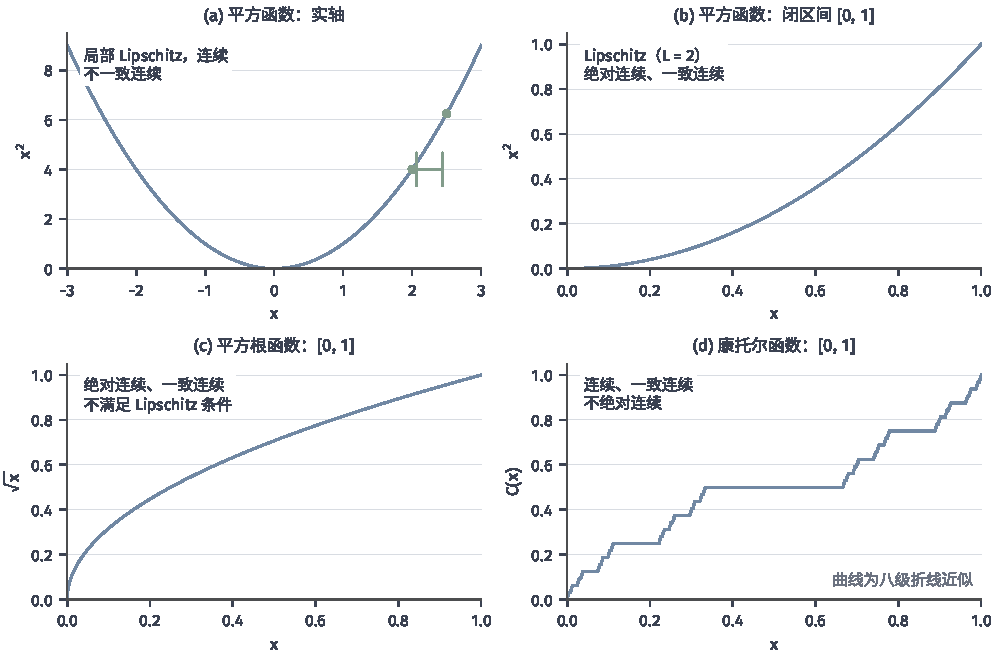
\includegraphics[width=169mm]{figures/01-mathematical-preliminaries-upper/01-mathematical-language-combinatorics-analysis-optimization/matplotlib/continuity-conditions/figure.pdf}
 \caption{连续性条件依赖于函数和定义域。(a)平方函数在实轴上连续且局部Lipschitz，但不一致连续；只展示$[-3,3]$内的曲线，标记对应$x_2=2$、$y_2=2+1/2$，完整反例使用$x_n=n$、$y_n=n+1/n$两列输入。(b)同一函数限制到$[0,1]$后为Lipschitz函数，因而绝对连续且一致连续。(c)$\sqrt x$在$[0,1]$上绝对连续、一致连续，却不是Lipschitz函数。(d)康托尔函数在$[0,1]$上连续且一致连续，但不绝对连续。右下曲线为八级折线近似，性质标注属于极限函数；每条有限折线本身都是Lipschitz函数，图形不能代替不绝对连续的证明。}
 \label{fig:analysis-continuity-conditions}
\end{figure*}

\subsection{闭区间上连续函数的性质}

\subsubsection{有界性与最值}
第~\ref{chap:sets-functions-and-proofs}章已经看到，函数的下确界未必能取到，例如$x$在$(0,1)$上没有最小值。所以在寻找最小值之前，需要先知道什么条件保证最值存在。
关键仍是收敛子列：在闭且有界的集合中，Bolzano--Weierstrass定理~\ref{thm:analysis-bounded-subsequence}给出每个序列的收敛子列，
闭集的序列判据（引理~\ref{lem:analysis-closed-sequence-criterion}）保证极限仍在集合内。
再结合连续性，就能证明函数有界并达到最值。
\begin{theorem}[闭有界集上的极值定理]
\label{thm:analysis-extreme-value}
设$K\subseteq\mathbb R$非空、闭且有界，$f:K\to\mathbb R$连续，则$f$有界，且在$K$上达到最小值和最大值。特别地，结论适用于非空闭区间。
\end{theorem}
\begin{proof}
先证有界。若$f$无界，可选$x_n\in K$使$|f(x_n)|>n$。$K$有界，序列$(x_n)$有收敛子列$x_{n_k}\to x$，闭性保证$x\in K$；连续性给出$f(x_{n_k})\to f(x)$。收敛数列有界，这与$|f(x_{n_k})|>n_k\to\infty$矛盾。

再证达到最小值。$f$有界且$K$非空，所以$m=\inf_K f$是有限实数。对每个$n$选$x_n\in K$使$m\leq f(x_n)<m+1/n$。取收敛子列$x_{n_k}\to x^\star\in K$，连续性给出$f(x_{n_k})\to f(x^\star)$；而$f(x_{n_k})$夹在$m$与$m+1/n_k$之间，也趋于$m$，所以$f(x^\star)=m$。对$-f$重复论证即得最大值。
\end{proof}
定理要求定义域闭、定义域有界且函数连续，三个条件缺一不可。下面三个函数各缺少其中一个条件，下确界都取不到。
\begin{example}[极值定理的条件]
\label{ex:analysis-extrema-failures}
定义域不闭：在$(0,1)$上，连续函数$f(x)=x$的下确界为$0$，但$0$不在定义域中，最小值不存在。

定义域无界：实轴闭但无界。$e^x$在$\mathbb R$上连续，$x\to-\infty$时趋于$0$，下确界为$0$；由于$e^x>0$，下确界取不到。

函数不连续：在$[0,1]$上令$f(0)=1$，$x>0$时$f(x)=x$。定义域闭且有界，但$x\downarrow0$时$f(x)\to0\neq f(0)$，$f$在$0$处不连续。下确界仍为$0$，而$f(0)=1$，$x>0$时$f(x)=x>0$，所以最小值不存在。
\end{example}
三个条件分别排除了一种失效方式：有界性保证序列有收敛子列，闭性保证子列的极限仍在定义域内，连续性保证函数值随子列收敛到极限点处的值。

\subsubsection{介值定理}
闭区间上的连续函数还有另一条性质：函数从一个端点值变到另一个端点值时，取遍二者之间的每个数值。
这一结论要求两个端点之间的整段都属于定义域，比极值定理的“闭且有界”更具体。
\begin{theorem}[闭区间上的介值定理]
\label{thm:analysis-intermediate-value}
设$a,b\in\mathbb R$、$a<b$，$f:[a,b]\to\mathbb R$连续。则
\[
 \begin{gathered}
 \forall c\in[\min\{f(a),f(b)\},\max\{f(a),f(b)\}],\\
 \exists\xi\in[a,b],\quad f(\xi)=c.
 \end{gathered}
\]
若$\min\{f(a),f(b)\}<c<\max\{f(a),f(b)\}$，则可取$\xi\in(a,b)$。
\end{theorem}
\begin{proof}
$c=f(a)$或$c=f(b)$时，直接取相应端点。下面设$f(a)<c<f(b)$，令
$S=\{x\in[a,b]:f(x)\leq c\}$。因为$a\in S$且$S$有上界$b$，实数的确界性质给出$u=\sup S\in[a,b]$。
对每个正整数$n$，可选$x_n\in S$满足$u-1/n<x_n\leq u$，于是$x_n\to u$。
连续性使$f(x_n)\to f(u)$，由$f(x_n)\leq c$得到$f(u)\leq c$；又因$f(b)>c$，所以$u\neq b$。
若$f(u)<c$，连续性保证$u$右侧充分近的点仍有函数值小于$c$；
由于$u<b$，可在$[a,b]$内选到这样的点$v>u$。于是$v\in S$，与$u$是$S$的上界矛盾。
因此$f(u)=c$。又因$f(a)<c$，有$u\neq a$，所以$u\in(a,b)$。
若$f(a)>c>f(b)$，对$-f$与$-c$应用同一论证即可。
\end{proof}
定理用到了两个端点之间的整段都属于定义域。定义域闭且有界但有缺口时，介值性可能失效。
\begin{example}[有缺口的定义域上不取中间值]
\label{ex:analysis-intermediate-value-gap}
令$X=[-2,-1]\cup[1,2]$，在$[-2,-1]$上取$f(x)=0$，在$[1,2]$上取$f(x)=1$。对每个$a\in X$取$\delta=1$：若$x\in X$且$|x-a|<1$，则$x$与$a$属于同一段，$f(x)=f(a)$。所以$f$在$X$上连续。$X$闭且有界，$f$在$-2$与$2$处分别取$0$和$1$，却不取中间值$1/2$。
\end{example}
极值定理在这个定义域上仍然成立；闭且有界足以保证最值，却不能代替介值定理中的区间条件。

\par\Needspace{10\baselineskip}
\section{微分的定义}
\label{sec:analysis-derivatives-linear-approximation}

连续性只说明输入接近时函数值也接近，没有说明函数值随输入变化的快慢。本节先用差商的极限定义导数，再把导数改写为函数增量的一阶线性近似，由此定义微分。

\subsection{导数}

\paragraph{差商}
设$f$在包含$a$的某个开区间内有定义。输入从$a$变为$a+h$时，函数增量为$\Delta f=f(a+h)-f(a)$。当$h\neq0$时，比值$\Delta f/h$称为差商，表示这两个输入之间的平均变化率；在图形上，它是连接$(a,f(a))$与$(a+h,f(a+h))$两点的割线斜率。

\paragraph{导数}
让$h$趋于零，两点之间的平均变化率就收缩为一点处的变化率。若差商在$h\to0$时趋于一个有限实数，就定义
\[
 f'(a)=\lim_{h\to0}\frac{f(a+h)-f(a)}h,
\]
称其为$f$在$a$处的\term{导数}（derivative），并称$f$在$a$处可导。导数给出该点的瞬时变化率，在图形上是该点切线的斜率。

若$f$在某个区间内每点都可导，则$a\mapsto f'(a)$又构成一个函数，称为导函数。例如$f(x)=x^2$时，差商$[(a+h)^2-a^2]/h=2a+h$，令$h\to0$得$f'(a)=2a$。

\paragraph{单侧导数}
在区间端点处，或在左右两侧变化方式不同的点处，需要分别考察两侧的差商。
只让$h>0$或只让$h<0$取极限，分别得到右导数$f'_+(a)$和左导数$f'_-(a)$。在内点处，双侧导数存在，当且仅当左右导数都存在、有限且相等。在闭区间端点讨论导数时，本章明确采用从区间内部取得的单侧导数；未特别说明时，内点处的导数都指有限的双侧导数。

\subsection{可微函数}

导数还可以写成函数增量的近似形式。差商趋于$f'(a)$，等价于$f(a+h)-f(a)-f'(a)h$除以$h$后趋于零，即
\begin{equation}
 f(a+h)=f(a)+f'(a)h+o(|h|),\qquad h\to0,
\label{eq:analysis-scalar-first-order}
\end{equation}
其中$o(|h|)$表示除以$|h|$后趋于零的量，沿用第~\ref{sec:comb-growth-scales}节的记号。

式~\eqref{eq:analysis-scalar-first-order}把函数增量分成线性部分$f'(a)h$与高阶余项。反过来，也可以不先假定导数存在，只要求增量有这样的分解：若存在实数$A$，使$h\to0$时$f(a+h)-f(a)=Ah+o(|h|)$，就称$f$在$a$处\term{可微}（differentiable）。两边除以$h$再令$h\to0$，可知差商趋于$A$，所以$f$在$a$处可导且$A=f'(a)$。结合式~\eqref{eq:analysis-scalar-first-order}，一元实函数在内点处可导与可微等价。

可微的分解中，线性部分把输入增量$h$映成函数增量的一阶预测值。线性映射$h\mapsto f'(a)h$称为$f$在$a$处的\term{微分}（differential），记为$\mathrm df_a(h)$。导数$f'(a)$是一个实数，微分则是以它为系数的线性映射。常用记号$\mathrm df=f'(x)\,\mathrm dx$表达同一关系，其中$\mathrm dx$表示输入增量。实际的有限增量$\Delta f$还包含余项，一般不等于微分。

微分与实际增量之差就是式~\eqref{eq:analysis-scalar-first-order}中的余项。用具体数值比较二者，可以看到余项有多大。
\begin{example}[平方函数在$a=3$处的微分]
\label{ex:analysis-square-differential}
设$f(x)=x^2$，$a=3$，则$f'(3)=6$，微分为$\mathrm df_3(h)=6h$。取$h=0.1$，微分给出$0.6$，实际增量为$3.1^2-3^2=0.61$。一般地，
\[
 (3+h)^2-3^2-6h=h^2,
\]
所以两者之差恰为$h^2$，$h=0.1$时为$0.01$。余项$h^2$除以$|h|$后趋于零，符合式~\eqref{eq:analysis-scalar-first-order}。
\end{example}
\begin{example}[$x^3-3x$在$a=1/2$处的一阶近似]
\label{ex:analysis-cubic-linear-approximation}
设$f(x)=x^3-3x$。由$(a+h)^3=a^3+3a^2h+3ah^2+h^3$，差商为$3a^2-3+3ah+h^2$，令$h\to0$得$f'(a)=3a^2-3$。取$a=1/2$，则$f(1/2)=-11/8$、$f'(1/2)=-9/4$，一阶近似为
\begin{equation}
 T_1(\tfrac12+h)=-\frac{11}{8}-\frac94h.
\label{eq:analysis-cubic-linear-model}
\end{equation}
取$h=0.1$，$T_1(0.6)=-1.600$，而$f(0.6)=0.216-1.8=-1.584$，近似值比真值小$0.016$。
\end{example}
第一例的余项恰为$h^2$；第二例余下的$0.016$来自函数图像的弯曲，第~\ref{sec:analysis-second-order-curvature}节将用二阶导数解释它。

可微还蕴含连续。若$f$在$a$处可微，由式~\eqref{eq:analysis-scalar-first-order}，$h\to0$时$f(a+h)-f(a)=f'(a)h+o(|h|)\to0$，即$f$在$a$处连续。

连续却只是可微的必要条件，并不充分。
\begin{example}[绝对值函数在原点连续而不可微]
\label{ex:analysis-absolute-value-not-differentiable}
设$f(x)=|x|$。由$\bigl||x|-|a|\bigr|\leq|x-a|$，$f$在每一点连续。在原点，差商为$|h|/h$：$h>0$时等于$1$，$h<0$时等于$-1$。所以$f'_+(0)=1$、$f'_-(0)=-1$，左右导数不相等，$f$在$0$处不可导，也就不可微。
\end{example}
阶跃函数在原点不连续，由上述必要条件，它在原点也不可微。图~\ref{fig:analysis-continuity-counterexamples}比较了连续且可微、连续但不可微与不连续三种情形。
\begin{figure*}[htbp]
 \centering
 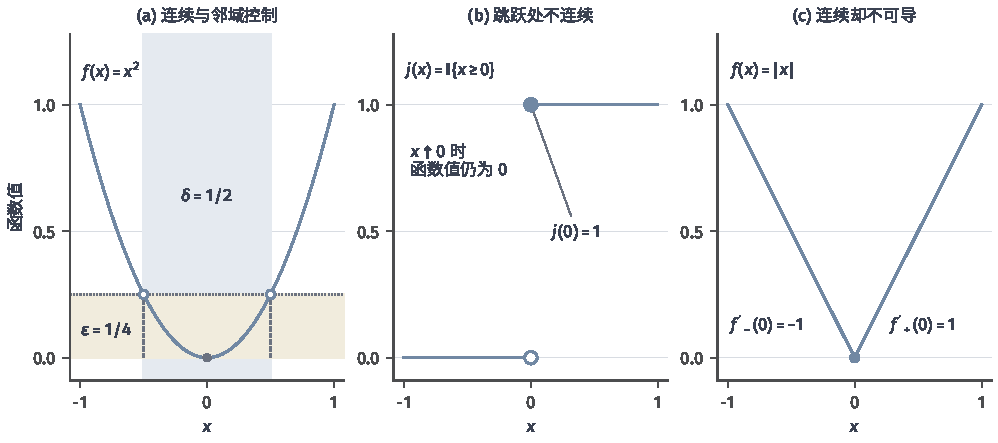
\includegraphics[width=169.0mm]{figures/01-mathematical-preliminaries-upper/01-mathematical-language-combinatorics-analysis-optimization/matplotlib/analysis-continuity-counterexamples/figure.pdf}
 \caption{平方函数、绝对值函数与阶跃函数在原点的差别。平方函数连续且可微；绝对值函数连续，但左右导数不同；阶跃函数的左右极限不同。连续性控制函数值的极限，可微性还要求差商具有同一个有限极限。}
 \label{fig:analysis-continuity-counterexamples}
\end{figure*}

\subsection{连续可微函数}

可导只要求每一点的差商各自有极限，并不要求邻近位置的导数接近该点的导数。
若进一步要求导函数本身连续，就得到更强的条件：若$f$在开区间$I$上可导且$f'$在$I$上连续，就称$f$连续可微，记为$f\in C^1(I)$。

在闭区间上使用$C^1([a,b])$时，要求$f$在$[a,b]$上连续、在$(a,b)$内可导，且$f'$能连续延拓到两个端点。由后文的Lagrange中值定理（定理~\ref{thm:analysis-lagrange-mean-value}）可以证明，延拓值就是相应的单侧导数。

处处可导与连续可微确实不同：导函数可能在某点不连续。
\begin{example}[处处可导而导函数不连续]
\label{ex:analysis-derivative-not-continuous}
令$f(0)=0$，$x\neq0$时$f(x)=x^2\sin(1/x)$。在原点，差商为$h\sin(1/h)$；由$|h\sin(1/h)|\leq|h|$及夹逼定理，它趋于$0$，所以$f'(0)=0$。在非零点，
\[
 f'(x)=2x\sin\frac1x-\cos\frac1x,
\]
这一公式将在示例~\ref{ex:analysis-oscillating-derivative-formula}中由求导规则得到。取$x_n=1/(2\pi n)$，则$x_n\to0$，而$\sin(1/x_n)=0$、$\cos(1/x_n)=1$，故$f'(x_n)=-1$。$f'(x_n)$不趋于$f'(0)=0$，所以$f'$在$0$处不连续：$f$在$\mathbb R$上处处可导，却不属于$C^1(\mathbb R)$。
\end{example}
导数在原点附近的振荡来自$-\cos(1/x)$一项，它在$-1$与$1$之间反复取值。因此$C^1$是比处处可导更强的条件。

\section{微分的运算法则}
\label{sec:analysis-scalar-chain-rules}

本节由已知函数的导数求组合函数的导数。以下设$f,g$在所讨论的点$a$的某个开邻域内有定义，并在$a$处可导；各条规则都由差商的极限或式~\eqref{eq:analysis-scalar-first-order}的一阶展开得到。

\subsection{四则运算的求导}

\paragraph{和与数乘}
和的差商等于两个差商之和，常数倍的差商等于差商的同一常数倍。令$h\to0$，由极限的和与数乘法则得到$(f+g)'(a)=f'(a)+g'(a)$与$(cf)'(a)=cf'(a)$，其中$c$为实常数。差$f-g=f+(-1)g$的导数由这两条合并得到。

\paragraph{乘积法则}
乘积的增量可以拆成三部分。记$\Delta f=f(a+h)-f(a)$、$\Delta g=g(a+h)-g(a)$，则
\[
 f(a+h)g(a+h)-f(a)g(a)=g(a)\,\Delta f+f(a)\,\Delta g+\Delta f\,\Delta g.
\]
由式~\eqref{eq:analysis-scalar-first-order}，前两项之和为$[f'(a)g(a)+f(a)g'(a)]h+o(|h|)$；两个增量都是$O(|h|)$，它们的乘积属于$O(h^2)$，也是$o(|h|)$。所以$fg$在$a$处可微，一次项的系数就是导数。连同上一段的和法则，得到
\begin{equation}
 \begin{aligned}
 (f+g)'(a)&=f'(a)+g'(a),\\
 (fg)'(a)&=f'(a)g(a)+f(a)g'(a).
 \end{aligned}
\label{eq:analysis-scalar-sum-product-rules}
\end{equation}

\paragraph{商法则}
设$g(a)\neq0$。可导蕴含连续，按商的连续性中的论证，$g$在$a$附近不为零，$f/g$在$a$附近有定义。先求倒数的导数：
\[
 \frac1h\Bigl(\frac1{g(a+h)}-\frac1{g(a)}\Bigr)
 =-\frac{g(a+h)-g(a)}h\cdot\frac1{g(a+h)g(a)}
 \longrightarrow-\frac{g'(a)}{g(a)^2},
\]
其中用到$g(a+h)\to g(a)$。再把$f/g$写成$f\cdot(1/g)$并使用乘积法则，得到
\[
 \left(\frac fg\right)'(a)
 =\frac{f'(a)}{g(a)}-\frac{f(a)g'(a)}{g(a)^2}
 =\frac{f'(a)g(a)-f(a)g'(a)}{g(a)^2}.
\]
条件$g(a)\neq0$既保证$f/g$在$a$附近有定义，也保证公式右侧有意义。

\subsection{复合函数求导}

复合函数的输入变化先经过内层，再传入外层；总的一阶变化由两层的局部变化率共同决定。
若$f$在$a$处可导，$g$在$f(a)$处可导，且$g\circ f$在$a$附近有定义，则
\begin{equation}
 (g\circ f)'(a)=g'(f(a))f'(a).
\label{eq:analysis-scalar-chain-rule}
\end{equation}
这称为\term{链式法则}（chain rule）。

证明时，记$b=f(a)$、$k(h)=f(a+h)-f(a)$。由$f$的一阶展开，$k(h)=f'(a)h+o(|h|)$，所以$k(h)\to0$，并且充分小的$h$满足$|k(h)|\leq(|f'(a)|+1)|h|$。把$g$在$b$处的一阶展开写成
\[
 g(b+k)=g(b)+g'(b)k+|k|\,\varepsilon(k),
\]
其中$k\neq0$时$\varepsilon(k)=[g(b+k)-g(b)-g'(b)k]/|k|$，它在$k\to0$时趋于零，并规定$\varepsilon(0)=0$。代入$k=k(h)$，得到
\[
 g(f(a+h))-g(f(a))=g'(b)f'(a)h+g'(b)\,o(|h|)+|k(h)|\,\varepsilon(k(h)).
\]
最后一项的绝对值不超过$(|f'(a)|+1)|h|\,|\varepsilon(k(h))|$，而$\varepsilon(k(h))\to0$，所以它也是$o(|h|)$。于是$g\circ f$在$a$处可微，一次项系数为$g'(f(a))f'(a)$。规定$\varepsilon(0)=0$使上式在$k(h)=0$时同样成立，所以证明也覆盖$f'(a)=0$等中间增量可能为零的情形，无需除以$k(h)$。

\subsection{反函数求导}
第~\ref{sec:analysis-inverse-continuity}节已经证明，区间上连续且严格单调的函数有连续的反函数。现在判断反函数何时可导，以及它的导数怎样由原函数的导数决定。

设$f:I\to J$在区间$I$上连续且严格单调，$J=f(I)$，其反函数为$g=f^{-1}$。设$a$是$I$的内点，$f$在$a$处可导且$f'(a)\neq0$，记$b=f(a)$。取$r>0$使$a-r,a+r\in I$；由介值定理，$J$包含$f(a-r)$与$f(a+r)$之间的整段，而$b$严格位于二者之间，所以$b$是$J$的内点。对充分小的$k\neq0$，令$h=g(b+k)-a$。$g$是一一对应，所以$h\neq0$；$g$连续，所以$k\to0$时$h\to0$。由$f(a+h)=b+k$，
\[
 \frac{g(b+k)-g(b)}k
 =\frac{h}{f(a+h)-f(a)}\longrightarrow\frac1{f'(a)}.
\]
因此$g$在$b$处可导，且$g'(b)=1/f'(a)$。

对恒等式$f(g(y))=y$使用链式法则，也会得到同一公式；但链式法则要求$g$已经可导，所以上面先用差商证明可导性。公式需要两个条件：$f$在所讨论的区间上一一对应，且在对应点处$f'(a)\neq0$。例如$x^3$在$0$处导数为零，其反函数$\sqrt[3]y$在$0$处的差商为$1/(\sqrt[3]k)^2$，$k\to0$时无界，所以反函数在$0$处不可导。

\subsection{基本初等函数的导数}
\label{sec:analysis-elementary-derivatives}

有了四则运算、复合与反函数的求导规则，复杂函数的求导就归结为少数基本函数的导数。以下逐类从差商推出这些导数，并注明成立范围。

\subsubsection{常数函数与整数幂函数}
常数函数$f(x)=c$的差商恒为零，恒等函数$f(x)=x$的差商恒为$1$，所以二者的导数分别为$0$和$1$。
对正整数$m$，把$x^m$看成$m$个恒等函数的乘积，反复使用乘积法则：每一项只对一个因子求导、保留其余$m-1$个因子，共有$m$项，每项都等于$x^{m-1}$，所以$(x^m)'=mx^{m-1}$。
$m=0$时$x^0=1$是常数函数，公式右侧按$0$理解。

对负整数$m=-n$（$n$为正整数），在$x\neq0$处把$x^m$写成$1/x^n$，由商法则，
\[
 \Bigl(\frac1{x^n}\Bigr)'=-\frac{nx^{n-1}}{x^{2n}}=-nx^{-n-1}=mx^{m-1},
\]
仍是同一形式。于是
\[
 \begin{aligned}
 (c)'&=0,\\
 (x^m)'&=mx^{m-1}\qquad(m\in\mathbb Z),
 \end{aligned}
\]
其中$m\geq0$时对全体实数$x$成立，$m<0$时要求$x\neq0$。

\subsubsection{正弦函数与余弦函数}
三角函数采用弧度制。第~\ref{sec:analysis-function-limits}节已经得到$\sin h/h\to1$与$(\cos h-1)/h\to0$。由正弦、余弦的加法公式，两个差商都能写成这两个比值的组合：
\[
 \begin{aligned}
 \frac{\sin(x+h)-\sin x}{h}
 &=\sin x\frac{\cos h-1}{h}+\cos x\frac{\sin h}{h}
 \longrightarrow\cos x,\\
 \frac{\cos(x+h)-\cos x}{h}
 &=\cos x\frac{\cos h-1}{h}-\sin x\frac{\sin h}{h}
 \longrightarrow-\sin x.
 \end{aligned}
\]
因此
\[
 \begin{aligned}
 (\sin x)'&=\cos x,\\
 (\cos x)'&=-\sin x,
 \end{aligned}
\]
两式对全体实数$x$成立。
若改用角度制，基本极限$\sin h/h$会多出比例系数$\pi/180$，导数公式也随之多出这个系数。

\subsubsection{指数函数}
自然指数函数满足$e^{x+h}=e^xe^h$。由第~\ref{sec:analysis-function-limits}节的基本极限$(e^h-1)/h\to1$，得到
\[
 \frac{e^{x+h}-e^x}{h}=e^x\frac{e^h-1}{h}\longrightarrow e^x.
\]
推导只用到由级数得到的乘法公式和这个基本极限，不依赖其他求导结果。因此
\[
 (e^x)'=e^x\qquad(x\in\mathbb R).
\]

\subsubsection{对数函数与实数幂函数}
自然对数定义为指数函数的反函数，先要确认这个反函数存在。$e^x$连续、严格递增且恒为正，$x\to-\infty$时趋于$0$，$x\to+\infty$时趋于$+\infty$。对任意$y>0$，先选两点使指数值分别小于和大于$y$，再用介值定理得到原像；严格递增保证原像唯一。所以指数函数是$\mathbb R$到$(0,\infty)$的一一对应，其反函数称为自然对数，记为$\log x$（也记$\ln x$），定义在$x>0$上。指数函数的导数$e^x$处处非零，由反函数求导，$(\log x)'=1/e^{\log x}=1/x$。

设$a>0$且$a\neq1$。实数次幂定义为$a^x=e^{x\log a}$，它的反函数$\log_a x$等于$(\log x)/(\log a)$，因为$a^{(\log x)/(\log a)}=e^{\log x}=x$。由链式法则，$(a^x)'=e^{x\log a}\log a=a^x\log a$；由数乘法则，$(\log_a x)'=1/(x\log a)$。
对任意实数$\alpha$，在$x>0$上定义$x^\alpha=e^{\alpha\log x}$，链式法则给出$(x^\alpha)'=e^{\alpha\log x}\cdot\alpha/x=\alpha x^{\alpha-1}$。于是
\[
 \begin{aligned}
 (\log x)'&=\frac1x, &&x>0,\\
 (\log_a x)'&=\frac1{x\log a}, &&x>0,\\
 (x^\alpha)'&=\alpha x^{\alpha-1}, &&x>0,\\
 (a^x)'&=a^x\log a, &&x\in\mathbb R.
 \end{aligned}
\]
这里没有为负数底数定义任意实数次幂，所以$x^\alpha$的公式只在$x>0$上使用。

\subsubsection{基本初等函数导数表}
表~\ref{tab:analysis-elementary-derivatives}汇总了上面得到的公式及成立范围。
把它们与四则运算法则、链式法则和反函数求导结合，就能求出由这些函数经有限次运算与复合得到的初等函数的导数。
示例~\ref{ex:analysis-derivative-not-continuous}在非零点使用的导数公式，就可以这样由乘积法则、链式法则和正弦导数得到。
\begin{example}[$x^2\sin(1/x)$在非零点的导数]
\label{ex:analysis-oscillating-derivative-formula}
设$x\neq0$。内层函数$1/x=x^{-1}$的导数为$-1/x^2$，由链式法则和正弦导数，$\bigl(\sin(1/x)\bigr)'=-\cos(1/x)/x^2$。再由乘积法则，
\[
 \Bigl(x^2\sin\frac1x\Bigr)'
 =2x\sin\frac1x+x^2\Bigl(-\frac1{x^2}\cos\frac1x\Bigr)
 =2x\sin\frac1x-\cos\frac1x.
\]
\end{example}
这些规则不能用于原点，因为$\sin(1/x)$在$0$处没有定义；原点处的导数须直接用差商计算，正如示例~\ref{ex:analysis-derivative-not-continuous}所做。
\begin{table}[htbp]
 \centering\small
 \begin{tabular}{@{}lll@{}}
 \toprule
 函数 & 导数 & 成立范围\\
 \midrule
 $c$ & $0$ & $x\in\mathbb R$\\
 $x^m$（$m\in\mathbb Z$） & $mx^{m-1}$ & $m\geq0$时$x\in\mathbb R$；$m<0$时$x\neq0$\\
 $x^\alpha$（$\alpha\in\mathbb R$） & $\alpha x^{\alpha-1}$ & $x>0$\\
 $\sin x$ & $\cos x$ & $x\in\mathbb R$\\
 $\cos x$ & $-\sin x$ & $x\in\mathbb R$\\
 $e^x$ & $e^x$ & $x\in\mathbb R$\\
 $a^x$（$a>0$，$a\neq1$） & $a^x\log a$ & $x\in\mathbb R$\\
 $\log x$ & $1/x$ & $x>0$\\
 $\log_a x$（$a>0$，$a\neq1$） & $1/(x\log a)$ & $x>0$\\
 \bottomrule
 \end{tabular}
 \caption{基本初等函数的导数。三角函数采用弧度制，$\log$为自然对数。}
 \label{tab:analysis-elementary-derivatives}
\end{table}

\section{闭区间上可微函数的性质}

导数记录一点处的变化率。本节把它与区间上的极值、端点之间的净变化以及两点之间的变化幅度联系起来。
涉及闭区间$[a,b]$的中值结论都只要求函数在$[a,b]$上连续、在$(a,b)$内可导，不要求端点处的单侧导数存在。

\subsection{局部极值与驻点}

\paragraph{局部极值}
导数只反映一点附近的变化，与它对应的是只比较邻近函数值的极值，而不是整个定义域上的最值。
设$c$属于$f$的定义域。若存在$r>0$，使定义域中所有满足$|x-c|<r$的$x$都有$f(x)\geq f(c)$，则称$c$为$f$的局部极小点；若其中$x\neq c$的点都满足严格不等式$f(x)>f(c)$，则称$c$为严格局部极小点。
把不等号反向，就得到局部极大点和严格局部极大点。

\paragraph{Fermat定理}
局部极值比较的是邻近的函数值，导数是差商的极限。在内点处可以从两侧取差商，差商的符号把这两种信息联系起来。
\begin{theorem}[Fermat定理]
\label{thm:analysis-fermat}
设$a<b$，$f:[a,b]\to\mathbb R$，$c\in(a,b)$。若$f$在$c$处可导，且$c$为$f$的局部极小点或局部极大点，则
\begin{equation}
 f'(c)=0.
\label{eq:analysis-scalar-first-order-necessary}
\end{equation}
\end{theorem}
\begin{proof}
设$c$为局部极小点。充分小的$h\neq0$满足$f(c+h)-f(c)\geq0$，
故$h>0$时差商非负，$h<0$时差商非正。
两侧差商趋于同一个有限导数，因而同时有$f'(c)\geq0$与$f'(c)\leq0$，即$f'(c)=0$。
局部极大点对$-f$应用同一论证即可。
\end{proof}
导数为零的点称为\term{驻点}（stationary point）。Fermat定理说明，内点处可导的局部极值点必为驻点。这一必要条件既不能逆用，也不能搬到端点上。
\begin{example}[非极值的驻点与端点处的极值]
\label{ex:analysis-fermat-condition-failures}
设$f(x)=x^3$。由$(x^3)'=3x^2$，$f'(0)=0$，所以$0$是驻点。但$x<0$时$f(x)<0=f(0)$，$x>0$时$f(x)>0=f(0)$；$0$的任何邻域内都有比$f(0)$更小和更大的函数值，所以$0$不是局部极值点。

再设$g(x)=x$，$x\in[0,1]$。$g$在端点$0$处取最小值，但右导数$g'_+(0)=1\neq0$。端点处只能从一侧取差商，Fermat定理证明中两侧差商的符号对比无法进行。
\end{example}
因此Fermat定理只给出内点处极值的必要条件。驻点是否为极值点，还要看函数在它两侧的增减；第~\ref{sec:analysis-monotonicity}节将用导数的符号判断这一点。

\subsection{中值定理}

\subsubsection{Rolle定理}
若函数在区间两端取同一值，整段的净变化为零。
在连续、可导的条件下，区间内部必有一点的瞬时变化率也为零。
\begin{theorem}[Rolle定理]
\label{thm:analysis-rolle}
设$a<b$，$f:[a,b]\to\mathbb R$在$[a,b]$上连续、在$(a,b)$内可导。
若$f(a)=f(b)$，则
\[
 \exists c\in(a,b),\qquad f'(c)=0.
\]
\end{theorem}
\begin{proof}
若$f$恒定，任取$c\in(a,b)$即可。
否则存在$x_0\in(a,b)$使$f(x_0)\neq f(a)$。
由闭区间上的极值定理~\ref{thm:analysis-extreme-value}，$f$在$[a,b]$上达到最大值和最小值。若$f(x_0)>f(a)=f(b)$，最大值不小于$f(x_0)$，严格大于两端的值，所以最大值必在某个内点达到；
若$f(x_0)<f(a)=f(b)$，同理最小值必在某个内点达到。
这个内点是局部极值点，$f$在那里可导，由Fermat定理~\ref{thm:analysis-fermat}，导数为零。
\end{proof}

\subsubsection{Lagrange中值定理}
两端取值不同时，可以先减去连接两个端点的直线，使剩余函数在两端相等，再对它应用Rolle定理。
这样就把整段的平均变化率与某个内点的瞬时变化率联系起来。
\begin{theorem}[Lagrange中值定理]
\label{thm:analysis-lagrange-mean-value}
设$a<b$，$f:[a,b]\to\mathbb R$在$[a,b]$上连续、在$(a,b)$内可导，则存在$c\in(a,b)$使
\begin{equation}
 f(b)-f(a)=f'(c)(b-a).
\label{eq:analysis-mean-value-theorem}
\end{equation}
等价地，$f'(c)=[f(b)-f(a)]/(b-a)$。
\end{theorem}
\begin{proof}
令
\[
 H(x)=f(x)-f(a)-\frac{f(b)-f(a)}{b-a}(x-a).
\]
$H$在$[a,b]$上连续、在$(a,b)$内可导，并满足$H(a)=H(b)=0$。
Rolle定理给出某个$c\in(a,b)$使
$H'(c)=f'(c)-[f(b)-f(a)]/(b-a)=0$，整理即得结论。
\end{proof}
这就是Lagrange\term{中值定理}（mean value theorem）的含义：区间上的平均变化率等于某个内点处的瞬时变化率。
定理只要求函数在每个内点可导，不要求导函数连续。

图~\ref{fig:analysis-process-mean-value-parallel}以$f(x)=x^2$、区间$[0,1]$为例：端点割线的斜率为$1$，$c=1/2$处的切线斜率$f'(1/2)=1$与之相等，两线平行。
\begin{figure}[!htbp]
 \centering
 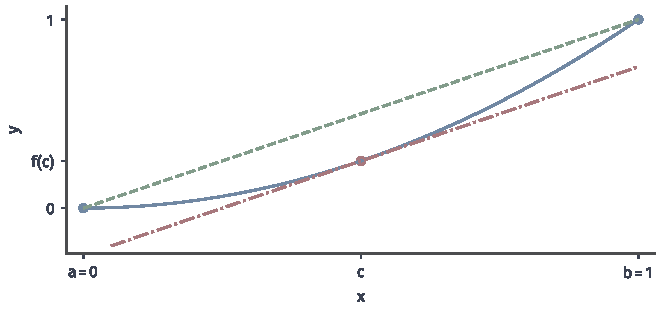
\includegraphics[width=112.0mm]{figures/01-mathematical-preliminaries-upper/01-mathematical-language-combinatorics-analysis-optimization/matplotlib/chapter3-concept-processes/mean-value-parallel.pdf}
 \caption{$f(x)=x^2$在$[0,1]$上，绿虚线为端点割线，红点划线为$c=1/2$处的切线。两线平行，因为$f'(c)=1=[f(1)-f(0)]/(1-0)$。两线高度不同：相等的是斜率，两条直线并不重合。}
 \label{fig:analysis-process-mean-value-parallel}
\end{figure}

\subsubsection{Cauchy中值定理}
比较两个函数在同一区间上的变化时，可以把两者的端点增量放进同一个辅助函数，再应用Rolle定理。
结论先写成交叉相乘的形式，这样不需要假设任何分母非零。
\begin{theorem}[Cauchy中值定理]
\label{thm:analysis-cauchy-mean-value}
设$a<b$，$f,g:[a,b]\to\mathbb R$均在$[a,b]$上连续、在$(a,b)$内可导，则存在$c\in(a,b)$使
\[
 (f(b)-f(a))g'(c)=(g(b)-g(a))f'(c).
\]
若进一步有$g'(x)\neq0$对每个$x\in(a,b)$成立，则$g(b)\neq g(a)$，并可写为
\[
 \frac{f(b)-f(a)}{g(b)-g(a)}=\frac{f'(c)}{g'(c)}.
\]
\end{theorem}
\begin{proof}
令
\[
 \begin{aligned}
 H(x)={}&(f(b)-f(a))(g(x)-g(a))\\
        &-(g(b)-g(a))(f(x)-f(a)).
 \end{aligned}
\]
$H$继承两函数的连续、可导条件，并有$H(a)=H(b)=0$。
应用Rolle定理得$H'(c)=0$，展开导数即为交叉相乘形式。
若$g'$在$(a,b)$内处处非零，$g(b)=g(a)$会使Rolle定理给出某个内点处$g'=0$，产生矛盾，故$g(b)\neq g(a)$。
此时$g'(c)\neq0$，交叉相乘形式两边同除以$(g(b)-g(a))g'(c)$，即得比值形式。
\end{proof}
取$g(x)=x$，则$g'=1$，比值形式就是Lagrange中值定理。

\subsection{单调性}
\label{sec:analysis-monotonicity}

\subsubsection{导数符号与单调性}
中值定理把任意两点之间的函数增量写成某个内点处的导数乘以输入增量，所以导数的符号可以控制整段的增减。
这里的关键是任意两点之间的整段都属于定义域。
\begin{theorem}[导数符号与单调性]
\label{thm:analysis-derivative-monotonicity}
设$a<b$，$f:[a,b]\to\mathbb R$在$[a,b]$上连续、在$(a,b)$内可导。
若$f'(x)\geq0$对所有$x\in(a,b)$成立，则$f$在$[a,b]$上单调不减；若处处有$f'(x)>0$，则严格递增。
相应地，$f'\leq0$蕴含单调不增，$f'<0$蕴含严格递减。
若$f'$在$(a,b)$内恒为零，则$f$在$[a,b]$上为常数。
\end{theorem}
\begin{proof}
任取$a\leq x<y\leq b$，在$[x,y]$上应用Lagrange中值定理，存在$\xi\in(x,y)$使
\[
 f(y)-f(x)=f'(\xi)(y-x).
\]
因为$y-x>0$，右侧的符号由$f'(\xi)$决定，于是得到四种单调性结论。
导数恒为零时，任意两点的函数值都相等，所以函数为常数。
\end{proof}
导数恒为零只保证函数在每个区间上为常数。若定义域由分离的区间组成，各段的常数未必相同：例如在$(0,1)\cup(2,3)$上，左段取$0$、右段取$1$的函数导数处处为零，却不是常数。中值定理不能跨过定义域的缺口使用。

导数为零也不妨碍严格单调：$x^3$在整个实轴上严格递增，因为$x<y$时$y^3-x^3=(y-x)(x^2+xy+y^2)>0$，但它在$0$处导数为零。因此“导数处处严格为正”是严格递增的充分条件，不是必要条件。

\subsubsection{驻点的一阶导数判别}
驻点条件本身不能判定极值，示例~\ref{ex:analysis-fermat-condition-failures}中的$x^3$在驻点$0$两侧都递增。
单调性定理把导数符号转化为增减方向，于是可以比较驻点两侧的变化：先降后升给出极小，先升后降给出极大。
\begin{theorem}[驻点的一阶导数判别]
\label{thm:analysis-first-derivative-test}
设$r>0$，$f$在$[c-r,c+r]$上连续、在$(c-r,c+r)$内可导，且$f'(c)=0$。
若
\[
 f'(x)<0\quad(c-r<x<c),\qquad
 f'(x)>0\quad(c<x<c+r),
\]
则$c$为$f$的严格局部极小点。
若两个区间上的导数符号分别为正和负，则$c$为$f$的严格局部极大点。
\end{theorem}
\begin{proof}
先考虑左负右正的情形。对$c-r<x<c$，$f$在$[x,c]$上连续，且在$(x,c)$内$f'<0$，由定理~\ref{thm:analysis-derivative-monotonicity}，$f$在$[x,c]$上严格递减，故$f(x)>f(c)$；
对$c<x<c+r$，在$[c,x]$上同理得到$f$严格递增，也有$f(x)>f(c)$。
所以$c$两侧充分近的异点都有更大的函数值，$c$为严格局部极小点。
左正右负时反向比较，得到$f(x)<f(c)$，因此$c$为严格局部极大点。
\end{proof}
判别法只需检查导数在驻点两侧的符号。导数能够因式分解时，各因子的符号就给出导数的符号。
\begin{example}[$x^3-3x$的驻点]
\label{ex:analysis-cubic-stationary-points}
设$f(x)=x^3-3x$，则$f'(x)=3x^2-3=3(x-1)(x+1)$，驻点为$x=\pm1$。在定理~\ref{thm:analysis-first-derivative-test}中取$r=1$。

对$x=1$：$0<x<1$时$x-1<0$、$x+1>0$，故$f'(x)<0$；$1<x<2$时两个因子都为正，故$f'(x)>0$。导数由负变正，$1$是严格局部极小点，$f(1)=-2$。

对$x=-1$：$-2<x<-1$时两个因子都为负，故$f'(x)>0$；$-1<x<0$时$x-1<0$、$x+1>0$，故$f'(x)<0$。导数由正变负，$-1$是严格局部极大点，$f(-1)=2$。

$1$只是局部极小点：$x\to-\infty$时$f(x)\to-\infty$，$f$在$\mathbb R$上没有最小值。
\end{example}
若导数在驻点两侧同号，例如$x^3$在$0$两侧都有$f'(x)=3x^2>0$，函数在驻点两侧沿同一方向变化，驻点就不是极值点。

\subsection{Lipschitz条件}

导数的符号控制增减方向；若还能统一限制导数的绝对值，就可以控制任意两点之间的变化幅度。
中值定理把这一导数上界直接转为第~\ref{sec:analysis-continuity-relations}节定义的Lipschitz条件。
\begin{theorem}[有界导数与Lipschitz条件]
\label{thm:analysis-bounded-derivative-lipschitz}
设$a<b$，$f:[a,b]\to\mathbb R$在$[a,b]$上连续、在$(a,b)$内可导。
若存在有限常数$L\geq0$使$|f'(x)|\leq L$对所有$x\in(a,b)$成立，则
\[
 \forall x,y\in[a,b],\qquad |f(y)-f(x)|\leq L|y-x|.
\]
即$f$在$[a,b]$上为Lipschitz连续函数，$L$是一个Lipschitz常数。
\end{theorem}
\begin{proof}
$x=y$时两侧都为零；$x<y$时，Lagrange中值定理给出$\xi\in(x,y)$，使
\[
 |f(y)-f(x)|=|f'(\xi)|\,|y-x|\leq L|y-x|.
\]
$x>y$时交换两点即可。
\end{proof}
例如$f(x)=x^2$在$(0,1)$内有$|f'(x)|=2x\leq2$，所以在$[0,1]$上可取$L=2$，与直接估计$|x^2-y^2|\leq2|x-y|$一致。
定理给出的是Lipschitz条件的充分条件；与单调性定理一样，它要求两点之间的整段都属于定义域。

若$f\in C^1([a,b])$，连续导数在闭区间上有界（极值定理~\ref{thm:analysis-extreme-value}），由上面的定理，$f$是Lipschitz连续函数；再由定理~\ref{thm:analysis-continuity-implications}，$f$绝对连续且一致连续。
反过来，Lipschitz连续不能保证导数处处存在：$|x|$在$[-1,1]$上Lipschitz连续，却在$0$处不可导（示例~\ref{ex:analysis-absolute-value-not-differentiable}）。
因此，函数值变化受控与经典导数处处存在是两种不同的条件，需要分别检查。

\section{高阶微分}

\subsection{高阶导数}

\paragraph{二阶导数}
要研究斜率本身怎样变化，可以继续对导函数求导。
若导函数$f'$在某点可导，它在该点的导数称为$f$的二阶导数，记为$f''$。例如$f(x)=x^3-3x$时，$f'(x)=3x^2-3$，$f''(x)=6x$。

\paragraph{高阶导数}
依次定义$f^{(r)}=(f^{(r-1)})'$，并约定$f^{(0)}=f$。
若$f$在开区间$I$上直到第$r$阶的导数都存在且连续，就称$f$为$r$阶连续可微函数，记为$f\in C^r(I)$，不致混淆时简写为$C^r$。$C^r([a,b])$在端点处的导数采用从内部取得的连续延拓，与$C^1([a,b])$的约定相同。

与一阶微分$\mathrm df=f'(x)\,\mathrm dx$对应，以$x$为自变量时，$r$阶微分记为$\mathrm d^rf=f^{(r)}(x)(\mathrm dx)^r$。它只给出第$r$阶变化的系数；用它近似实际增量时，还需要Taylor公式中的阶乘因子与余项。

\subsection{Taylor公式}
\label{sec:analysis-taylor-approximation}

一阶近似只用到一阶导数。要提高精度，可以依次加入二阶、三阶等高阶项，同时估计截去部分的误差。本节先用一个例子观察二次项补充了什么，再给出一般阶数的Taylor公式及其两种余项。

\subsubsection{二阶近似}
\label{sec:analysis-second-order-curvature}
示例~\ref{ex:analysis-cubic-linear-approximation}中，$x^3-3x$在$1/2$处的一阶近似在$h=0.1$时比真值小$0.016$。一阶近似只用了函数值和斜率；加入由二阶导数确定的二次项，可以看出这部分误差的来源。
\begin{example}[$x^3-3x$在$a=1/2$处的二阶近似]
\label{ex:analysis-cubic-quadratic-approximation}
仍设$f(x)=x^3-3x$。由$f''(x)=6x$，得$f''(1/2)=3$。在式~\eqref{eq:analysis-cubic-linear-model}上加入二次项$\tfrac12f''(1/2)h^2=\tfrac32h^2$，得到
\begin{equation}
 T_2(\tfrac12+h)=-\frac{11}{8}-\frac94h+\frac32h^2.
\label{eq:analysis-cubic-quadratic-model}
\end{equation}
取$h=0.1$，二次项为$0.015$，$T_2(0.6)=-1.585$，与真值$f(0.6)=-1.584$相差$0.001$。一阶近似的误差$0.016$中，二次项补上了$0.015$。
\end{example}
正的二阶导数说明斜率随$x$增加，曲线在$x=1/2$附近向上弯曲；二次项$\tfrac12f''(1/2)h^2$补上的正是切线近似遗漏的这部分弯曲。图~\ref{fig:analysis-derivative-orders}比较了两阶近似及其余项。
$T_1$与$T_2$分别是下面Taylor多项式在$r=1,2$时的特例。

\subsubsection{Lagrange余项}
要把上面的近似推广到任意阶，还需要控制截去的误差。设$r\geq0$为整数，$f$在$x_0$处$r$阶可导，称
\[
 T_r(x_0+h)=\sum_{k=0}^r\frac{f^{(k)}(x_0)}{k!}h^k
\]
为$f$在$x_0$处的$r$阶\term{Taylor多项式}（Taylor polynomial）。把它看作$x=x_0+h$的多项式，它在$x_0$处与$f$具有相同的函数值和前$r$阶导数。

截去的误差$f(x_0+h)-T_r(x_0+h)$称为余项。下面的\term{Taylor公式}（Taylor formula）用某个中间点处的高阶导数表示余项。
\begin{theorem}[带Lagrange余项的Taylor公式]
\label{thm:analysis-taylor-lagrange}
设$r\geq0$为整数，$x_0\in\mathbb R$，$h\neq0$，$f$在包含$x_0$与$x_0+h$之间闭线段的某个开区间上属于$C^{r+1}$。则存在严格位于$x_0$与$x_0+h$之间的$\xi$，使
\begin{equation}
 f(x_0+h)=\sum_{k=0}^r\frac{f^{(k)}(x_0)}{k!}h^k
 +\frac{f^{(r+1)}(\xi)}{(r+1)!}h^{r+1}.
\label{eq:analysis-taylor-arbitrary-order}
\end{equation}
最后一项称为Lagrange余项。若该线段上$|f^{(r+1)}|\leq M$，则
\[
 \bigl|f(x_0+h)-T_r(x_0+h)\bigr|\leq\frac{M|h|^{r+1}}{(r+1)!}.
\]
\end{theorem}
\begin{proof}
记$T_r(t)=\sum_{k=0}^rf^{(k)}(x_0)(t-x_0)^k/k!$，$R=f(x_0+h)-T_r(x_0+h)$，并令
\[
 H(t)=f(t)-T_r(t)-R\frac{(t-x_0)^{r+1}}{h^{r+1}}.
\]
$H$在$x_0$与$x_0+h$处都为零；由于$T_r$在$x_0$处与$f$有相同的前$r$阶导数，$r\geq1$时还有$H'(x_0)=\cdots=H^{(r)}(x_0)=0$。
先在$x_0$与$x_0+h$之间对$H$用Rolle定理，得到严格位于两者之间的$\xi_1$，使$H'(\xi_1)=0$。若$r\geq1$，再在$x_0$与$\xi_1$之间对$H'$用Rolle定理，得到$\xi_2$，使$H''(\xi_2)=0$。如此继续，第$k$次得到严格位于$x_0$与$\xi_{k-1}$之间的$\xi_k$，使$H^{(k)}(\xi_k)=0$。
共用$r+1$次后，$\xi=\xi_{r+1}$严格位于$x_0$与$x_0+h$之间；又因$T_r$是$r$次多项式，$T_r^{(r+1)}=0$，所以
\[
 0=H^{(r+1)}(\xi)=f^{(r+1)}(\xi)-\frac{(r+1)!}{h^{r+1}}R.
\]
整理即得公式。$r=0$时只用一次Rolle定理；$h<0$时“之间”指以$x_0+h$为左端点的区间，论证相同。误差界由$|f^{(r+1)}(\xi)|\leq M$直接得到。
\end{proof}
$r=0$时公式化为$f(x_0+h)=f(x_0)+f'(\xi)h$，这正是Lagrange中值定理的结论，不过那里只要求函数连续且在内部可导。
误差界说明，Taylor多项式的精度同时取决于阶数、位移大小和高阶导数的界。第~\ref{sec:analysis-integration-remainders}节还将用分部积分把余项写成积分，这里的证明不依赖积分。

多项式的高阶导数最终为零，Taylor公式可以逐项核对。
\begin{example}[$x^3-3x$在$x_0=1/2$处的余项]
\label{ex:analysis-cubic-taylor-remainders}
设$f(x)=x^3-3x$，$x_0=1/2$。除前面得到的$f(1/2)=-11/8$、$f'(1/2)=-9/4$、$f''(1/2)=3$外，还有$f'''\equiv6$，四阶及以上导数为零。对$r=3$应用定理~\ref{thm:analysis-taylor-lagrange}，余项含因子$f^{(4)}(\xi)=0$，所以三阶Taylor多项式就是$f$本身：
\[
 f(\tfrac12+h)=-\frac{11}{8}-\frac94h+\frac32h^2+h^3.
\]
直接展开$(\tfrac12+h)^3-3(\tfrac12+h)$也得到同一结果。与式~\eqref{eq:analysis-cubic-linear-model}和式~\eqref{eq:analysis-cubic-quadratic-model}比较，一阶Taylor多项式$T_1$遗漏$\tfrac32h^2+h^3$，二阶Taylor多项式$T_2$只遗漏$h^3$。后者正是$r=2$时的Lagrange余项：无论中间点$\xi$取在何处，都有$f'''(\xi)h^3/3!=h^3$。
\end{example}
图~\ref{fig:analysis-derivative-orders}的右图画出了这两个余项。$h$接近零时，$\tfrac32h^2+h^3=h^2(\tfrac32+h)$为正，真值位于$T_1$上方；$h^3$与$h$同号，真值在$h>0$时位于$T_2$上方，在$h<0$时位于下方。余项的阶数越高，它在$h=0$附近趋于零越快。
\begin{figure*}[htbp]
 \centering
 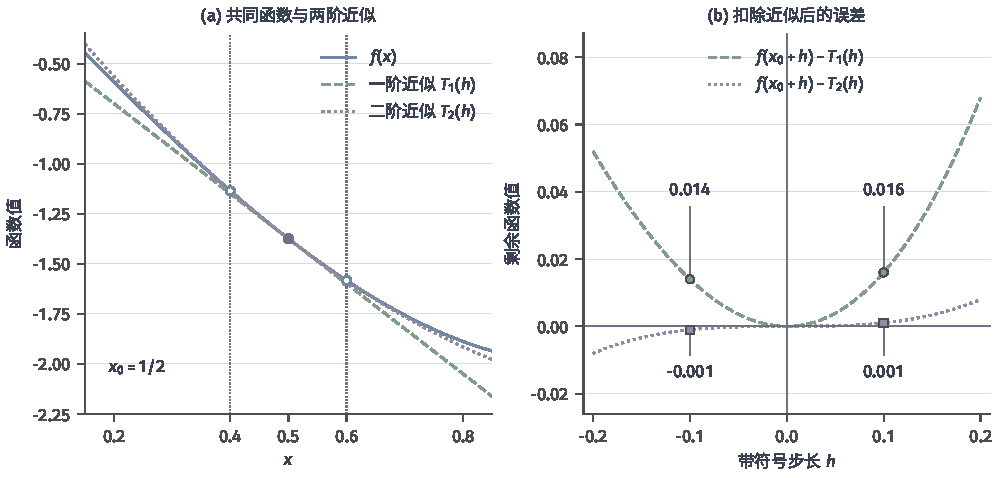
\includegraphics[width=169.0mm]{figures/01-mathematical-preliminaries-upper/01-mathematical-language-combinatorics-analysis-optimization/matplotlib/analysis-derivative-orders/figure.pdf}
 \caption{$f(x)=x^3-3x$在$x_0=1/2$处的Taylor近似，$h=x-x_0$。左图比较原函数、切线近似$T_1$与二次近似$T_2$；右图给出相应的带符号余项$3h^2/2+h^3$和$h^3$。标记点对应$h=\pm0.1$，余项的正负说明真值位于近似值的哪一侧。}
 \label{fig:analysis-derivative-orders}
\end{figure*}

\subsubsection{Peano余项}
如果只关心位移趋于零时误差的阶，可以不保留中间点，改用小量记号描述余项。
若$r\geq1$，$f$在包含$x_0$的某个开区间上属于$C^r$，则$h\to0$时
\[
 f(x_0+h)=\sum_{k=0}^r\frac{f^{(k)}(x_0)}{k!}h^k+o(|h|^r),
\]
称为带Peano余项的$r$阶Taylor公式。

推导时，对$r-1$阶Taylor公式使用Lagrange余项（这时定理~\ref{thm:analysis-taylor-lagrange}只要求$C^r$），得到$f(x_0+h)=T_{r-1}(x_0+h)+f^{(r)}(\xi_h)h^r/r!$，其中$\xi_h$位于$x_0$与$x_0+h$之间。把末项写成$f^{(r)}(x_0)h^r/r!$与$[f^{(r)}(\xi_h)-f^{(r)}(x_0)]h^r/r!$之和：前者与$T_{r-1}(x_0+h)$合成$T_r(x_0+h)$；后者除以$|h|^r$后趋于零，因为$\xi_h\to x_0$且$f^{(r)}$连续。这样就得到上式。

Peano余项描述局部误差的阶；若需要有限位移下的具体误差界，应使用Lagrange余项。$r=1$时上式就是式~\eqref{eq:analysis-scalar-first-order}，不过式~\eqref{eq:analysis-scalar-first-order}只需要$f$在该点可导。

\subsection{驻点的二阶导数判别}
在驻点处，Taylor公式的一阶项为零，函数在附近的增减就由二阶项决定。
设$a$是$f$的驻点，$f$在包含$a$的某个开区间上属于$C^2$。带Lagrange余项的一阶Taylor公式给出
\[
 f(a+h)-f(a)=\tfrac12f''(\xi_h)h^2,
\]
其中$\xi_h$位于$a$与$a+h$之间。若$f''(a)>0$，由$f''$的连续性，$h$充分小时$f''(\xi_h)\geq f''(a)/2>0$，所以每个充分小的非零$h$都使函数值严格增加，$a$为严格局部极小点。$f''(a)<0$时同理，$a$为严格局部极大点。

反之，在上述$C^2$条件下，局部极小点必须有$f''(a)\geq0$：若$f''(a)<0$，上一段说明$a$是严格局部极大点，附近其他点的函数值都严格小于$f(a)$，与局部极小矛盾。同理，局部极大点必须有$f''(a)\leq0$。

$f''(a)=0$时判别法没有结论：只知道前两阶导数，无法区分极小、极大与非极值。
\begin{example}[二阶导数为零时无法判别]
\label{ex:analysis-second-derivative-test-inconclusive}
考虑$x^4$、$-x^4$与$x^3$。三者在原点的一阶、二阶导数都为零：$(x^4)'=4x^3$、$(x^4)''=12x^2$，$(x^3)'=3x^2$、$(x^3)''=6x$，$-x^4$的导数只差一个符号。可是$x\neq0$时$x^4>0$，所以$0$是$x^4$的严格局部极小点；同理，$0$是$-x^4$的严格局部极大点；示例~\ref{ex:analysis-fermat-condition-failures}已说明$0$不是$x^3$的极值点。
\end{example}
回到示例~\ref{ex:analysis-cubic-stationary-points}，$f(x)=x^3-3x$有$f''(x)=6x$，$f''(1)=6>0$、$f''(-1)=-6<0$。二阶判别同样给出$1$为严格局部极小点、$-1$为严格局部极大点，与一阶导数判别的结论一致。

\FloatBarrier

\section{集合的测量}
\label{sec:comb-set-measurement}
\label{sec:analysis-set-structures}

区间$[a,b]$的长度是$b-a$，但实轴上的集合未必是一个区间。
本节要解决的问题是：怎样把区间的长度推广到更一般的实数集合，并在原来的区间上仍得到$b-a$？
本章后面的积分需要这样的长度：把输入范围分成若干块后，只有知道各块的大小，才能按这些大小累计函数取值。
有限集合的元素个数与加权计数是另一类测量，可以先用它们说明为集合赋予大小时应遵守的相加规则。

集合的大小与点之间的距离是两种不同的结构。
在同一条实轴上使用同一种通常距离，既可以测量区间的长度，也可以数集合中的点；
因此，选定度量并不能唯一确定测度，即给集合赋予大小的方式。

本节先用有限集合的计数与加权计数说明相加规则，再从区间长度构造Jordan测量；有理点集将说明，只用有限个区间逼近还不够。
为此，随后利用可数集的列举规则改用可数覆盖，定义勒贝格外测度。
外测度对每个集合都有定义，却不保证不交部分精确相加，所以再用精确分割条件选出可测集，在可测集上得到可数可加的勒贝格测度。
最后推导勒贝格测度在集合列、零测集与几乎处处方面的性质，并用康托尔集说明零测集可以不可数。

\subsection{有限集与Jordan测量}
\label{sec:comb-counting-to-weight}

我们先把目标限制在有界的实数集合上，希望给这些集合建立与区间长度相容的测量方法。
例如$[0,1]\cup[2,3]$由两段互不重叠、长度各为$1$的区间组成，总长度应为$2$。
由这个例子可以看出所求测量应满足的一条规则：集合分成有限个两两不交的部分时，总量等于各部分测量值之和。

下面先在有限集合上用计数和加权计数说明这条规则，再回到实轴。
实轴上的长度将从区间出发：先计算有限个区间的并，再用这些简单集合从内、外两侧逼近更一般的有界集合；
只有当内部与外部的长度估计逼近同一个数时，才用这个数定义集合的Jordan测量。

\subsubsection{有限集的测量}

\paragraph{计数与加权计数}

在有限集合上，最直接的测量是数元素个数；若不同元素代表不同的份量，还可以给每个元素指定权重。
设$X=\{x_1,\ldots,x_m\}$中的点互异，每点带有非负权重$w_i$。
把落在$A\subseteq X$中的点的权重相加，定义
\[
 \mu(A)=\sum_{i:x_i\in A}w_i.
\]
所有$w_i=1$时，$\mu(A)=|A|$，即元素个数；改变权重时，元素不变，测量值却可以改变。
例如在$X=\{a,b\}$上给$a,b$分别指定权重$1,2$，就有$\mu(\{a\})=1$、$\mu(\{b\})=2$、$\mu(X)=3$。

若$A_1,\ldots,A_k$两两不交，并集中的每个点恰好落入其中一组，它的权重在等式两侧都只计一次，故
\[
 \mu\left(\bigcup_{j=1}^k A_j\right)=\sum_{j=1}^k\mu(A_j).
\]
这称为\term{有限可加性}（finite additivity）。它沿用计数的加法规则，
但相加的是各组的权重，不必是元素个数。

\paragraph{集合权重与函数值}

$\mu(A)$只测量集合$A$本身。后面还要在集合上累计函数取值，届时每个点的贡献等于函数值乘以该点的权重。
下面在同一个两点集合上比较等权与加权两种累计。
\begin{example}[两点集合上的等权与加权累计]
沿用$X=\{a,b\}$，给$a,b$分别指定权重$1,2$，并取函数值$f(a)=3$、$f(b)=-1$。

每点计$1$时，集合大小为$|X|=2$，函数的取值和为$f(a)+f(b)=3-1=2$。

按权重计时，集合大小为$\mu(X)=1+2=3$，函数的加权和为
\[
 3\cdot1+(-1)\cdot2=1.
\]
\end{example}

同一组元素和同一组函数值，在两种权重下给出不同的集合大小（$2$与$3$），也给出不同的累计值（$2$与$1$）。
表~\ref{tab:analysis-metric-measure-integral}汇总这些计算；本章后面的积分将把这种加权累计推广到更一般的集合与函数。
\begin{table}[htbp]
 \centering\small
 \begin{tabularx}{\linewidth}{@{}lXX@{}}
 \toprule
 考察对象 & 所用规则 & $X=\{a,b\}$上的结果\\
 \midrule
 元素个数 & 每点计$1$ & $|X|=2$\\
 集合权重 & $a,b$分别计$1,2$ & $\mu(X)=3$\\
 数值的等权累计 & 取值为$3,-1$ & $3-1=2$\\
 数值的加权累计 & 同一取值采用权重$1,2$ & $3-2=1$\\
 \bottomrule
 \end{tabularx}
 \caption{有限计数与加权累计。相同的元素范围和相同的数值取值仍可采用不同权重；只有先固定权重，累计值才有确定含义。}
 \label{tab:analysis-metric-measure-integral}
\end{table}

\paragraph{点数与长度}

有限集合的例子说明了不交部分如何相加，但每点计$1$的规则不能给出区间长度。
例如$[0,1]$和$[0,2]$都含有无限多个点，逐点计数都得到无穷，而它们的长度分别应为$1$和$2$。
所以，要推广区间长度，必须另行规定与几何长度相容的测量规则。

单点$[a,a]$的长度为$0$，有限个单点的并也应有长度$0$。
这与非退化区间的长度为正并不矛盾：非退化区间含无限多个点，不能写成有限个单点的并，所以有限可加性不适用于把它拆成全部单点的操作。
第~\ref{sec:analysis-countable-outer-measure}节讨论可数覆盖时还要用到另一事实：非退化区间的点也不能列成一个序列。

因此我们改以区间长度为起点：先计算能由有限个区间组成的集合的长度，再研究不能这样表示的集合。

\subsubsection{Jordan测量}

\paragraph{区间长度与初等集}

一个区间的长度由端点决定；有限个区间组成的集合，也可以先拆成互不重叠的小段再相加。
对端点为$a\leq b$的有界区间$I$，规定长度为$\ell(I)=b-a$，不因端点是否包含而改变；
单点与空集的长度为$0$。

为反复使用这类可以直接计算长度的集合，先给它们一个名称：
我们把有限个这样的区间的并称为\term{初等集}（elementary set），空集也约定为初等集。
例如$[0,1]\cup[2,3]$是初等集，两段长度相加得到$2$。
区间发生重叠时，需要先消除重复计算：$[0,2]\cup[1,3]=[0,3]$的长度为$3$，不能把原来两段的长度直接相加为$4$。

一个初等集$B$可以有多种区间表示，所以先按一种表示规定长度，再检查结果与表示无关。
取定一种表示，将其中所有端点排序，按相邻端点之间的开区间及端点本身切分，得到有限个两两不交的小段；把属于$B$的小段长度相加，记为$\ell(B)$。
若采用另一种表示，把两组端点合在一起排序，便得到两种切分的共同细分。
区间从$c$处分成两段时，$(c-a)+(b-c)=b-a$，所以细分不改变总长度。
因此，两种表示给出同一个$\ell(B)$。

对有限个初等集取它们端点的共同细分可知，初等集的并、交、差仍为初等集，不交初等集的长度有限可加。
一般的有限覆盖只给出不等式：若$B\subseteq\bigcup_{j=1}^k B_j$，则
$\ell(B)\leq\sum_{j=1}^k\ell(B_j)$，因为在共同细分下，$B$的每个小段在右侧至少计算一次，重叠的小段还会被重复计算。
特别地，取$k=1$可知$A\subseteq B$时$\ell(A)\leq\ell(B)$。

\paragraph{内容量与外容量}

初等集的长度已经可以计算，但有界集合只要求一个集合包含在某个有限区间内，并不要求它本身由有限个区间组成。
下面的倒数点集就是这样的集合。
\begin{example}[倒数点集不是初等集]
\label{ex:set-measure-reciprocal-not-elementary}
考虑
\[
 E=\{1,1/2,1/3,\ldots\}\subseteq[0,1].
\]
它包含于$[0,1]$，因此有界。

对任意$u>0$，$E\cap[u,1]$中的点$1/n$都满足$n\leq1/u$，所以这一部分只有有限多个点。

由此可知$E$不包含任何正长度区间。假如$E$包含端点为$c<d$的区间，由$E\subseteq(0,1]$可知$c\geq0$；
取$u=(c+d)/2>0$，区间中的$[u,d)$便落在$E\cap[u,1]$中。它含无限多个点，与上一步的有限性矛盾。

若$E$是初等集，组成它的每个区间都包含于$E$，只能是单点或空集，于是$E$只有有限多个点；这与$E$含无限多个点矛盾。
所以$E$不是初等集。
\end{example}

因此初等集的长度公式不能直接用于$E$。
为了测量$E$这样的集合，一种办法是保留初等集作为计算工具，用包含关系给出长度估计。
把初等集$A$放在$E$内部，即$A\subseteq E$，$\ell(A)$就应是$E$的长度的下界；
用初等集$B$包住$E$，即$E\subseteq B$，$\ell(B)$就应是上界。
我们希望内部估计尽可能大、外部估计尽可能小，因此分别取内部长度的上确界与外部长度的下确界。
这两个数未必相等；若相等，内部与外部的估计就共同确定了一个长度值，可以把它作为$E$的测量值。

下面给这两个界命名，并按它们是否相等规定哪些有界集合可以用这种方法测量；两侧的候选都是初等集，长度都按初等集的长度$\ell$计算。
\begin{definition}[Jordan内容量与外容量]
\label{def:analysis-jordan-content}
对有界集合$E\subseteq\mathbb R$，定义\term{Jordan内容量}（Jordan inner content）与\term{Jordan外容量}（Jordan outer content）为
\[
 \begin{aligned}
 j_*(E)&=\sup\{\ell(A):A\subseteq E,\ A\text{为初等集}\},\\
 j^*(E)&=\inf\{\ell(B):E\subseteq B,\ B\text{为初等集}\}.
 \end{aligned}
\]
若$j_*(E)=j^*(E)$，称$E$为Jordan可测集，二者的共同值记为$j(E)$，称为它的\term{Jordan测量}（Jordan measure）值。
\end{definition}

对有界集合$E$，有界性保证外部候选非空且长度有限，空集则是内部候选；
又由$A\subseteq E\subseteq B$和初等集长度的单调性得$\ell(A)\leq\ell(B)$。所以
$0\leq j_*(E)\leq j^*(E)<\infty$。
上下确界一般不要求由某个最佳初等集取得；若$E$本身是初等集，内外都可以取$E$，结合$\ell(A)\leq\ell(E)\leq\ell(B)$便得$j_*(E)=j^*(E)=\ell(E)$。
所以新的定义保留了区间长度与有限区间并的长度，有限点集的测量值也仍为$0$。

倒数点集虽然不是初等集，它的两个容量却可以直接算出。
\begin{example}[倒数点集的Jordan测量为零]
\label{ex:set-measure-reciprocal-jordan-null}
仍取$E=\{1/n:n\geq1\}$。

内部：示例~\ref{ex:set-measure-reciprocal-not-elementary}已说明$E$不含正长度区间，所以包含于$E$的初等集只能由有限个单点组成，长度为$0$。于是
\[
 j_*(E)=0.
\]

外部：对每个整数$N\geq2$，取
\[
 B_N=\{1,1/2,\ldots,1/(N-1)\}\cup[0,1/N].
\]
前$N-1$个点分别由单点覆盖，其余的点$1/n$（$n\geq N$）全部落在$[0,1/N]$内，故$E\subseteq B_N$。
$B_N$是初等集，有限个单点不增加长度，所以$\ell(B_N)=1/N$。
于是$0\leq j^*(E)\leq1/N$对所有$N\geq2$成立，从而
\[
 j^*(E)=0.
\]

内外容量相等，所以$E$是Jordan可测集，且$j(E)=0$。
\end{example}

这个不属于初等集的无限点集仍然Jordan可测。
它的测量值来自有限逼近：外部候选的长度$1/N$可以任意小，内部候选的长度始终为$0$。

\paragraph{有限逼近与可加性}

内外数值相等也可以改写成误差条件：$E$为Jordan可测集，当且仅当对每个$\varepsilon>0$，
存在初等集$A\subseteq E\subseteq B$，使$\ell(B)-\ell(A)<\varepsilon$。
若$E$可测，按上确界和下确界的定义，各选一个与共同值$j(E)$相差小于$\varepsilon/2$的内部候选和外部候选即可。
反过来，若对每个$\varepsilon$都有这样的$A,B$，则$\ell(A)\leq j_*(E)\leq j^*(E)\leq\ell(B)$，两个容量之差小于任意正数，只能相等。

这个误差条件还保证有限次集合运算保持Jordan可测性。
分别以$A_E\subseteq E\subseteq B_E$和$A_F\subseteq F\subseteq B_F$夹住两个Jordan可测集，
它们的并夹在$A_E\cup A_F$与$B_E\cup B_F$之间，且
\[
 (B_E\cup B_F)\setminus(A_E\cup A_F)\subseteq(B_E\setminus A_E)\cup(B_F\setminus A_F).
\]
初等集$A\subseteq B$时，有限可加性给出$\ell(B)-\ell(A)=\ell(B\setminus A)$；再用有限覆盖不等式，新上下界的长度差不超过原来两份误差之和。

交集夹在$A_E\cap A_F$与$B_E\cap B_F$之间，差集$E\setminus F$夹在$A_E\setminus B_F$与$B_E\setminus A_F$之间。
两种情形中，外部逼近与内部逼近之差同样包含于$(B_E\setminus A_E)\cup(B_F\setminus A_F)$。
因此，Jordan可测集的有限并、交、差仍Jordan可测。

若$E,F$还不交，内部逼近$A_E,A_F$也不交。左端用不交初等集的有限可加性，右端用有限覆盖不等式，得到
\[
 \ell(A_E)+\ell(A_F)
 \leq j_*(E\cup F)\leq j^*(E\cup F)
 \leq\ell(B_E)+\ell(B_F).
\]
让各份逼近误差趋于零，两端都趋于$j(E)+j(F)$，所以$j(E\cup F)=j(E)+j(F)$。
这就是Jordan测量的有限可加性。论证中只合并了有限份逼近误差，所以它不能直接推广到无限多个集合的并。

\subsubsection{Jordan测量的局限}

\paragraph{有理点集的内外容量}

倒数点集$E$虽然不是初等集，仍能用有限区间并把外部长度压到任意小。
这是否意味着每个有界集合都能这样处理？下面考察$Q_0=\mathbb Q\cap[0,1]$，它将说明Jordan方法使用的有限逼近不能处理任意的有界集合。

先看$Q_0$在区间中的分布：任意非退化实区间$(a,b)$（$a<b$）都含有理数和无理数。
找有理数时，取正整数$q>1/(b-a)$，使相邻分数$p/q$与$(p+1)/q$的间距$1/q$小于区间长度。
令$p$为满足$p>aq$的最小整数，则$(p-1)/q\leq a<p/q$，于是$p/q\leq a+1/q<b$，即$p/q\in(a,b)$。

找无理数时，对区间内的有理数$r$，取正整数$k$使$\sqrt2/k<b-r$，则$r+\sqrt2/k$位于$(r,b)$内；
它若是有理数，$\sqrt2=k\bigl((r+\sqrt2/k)-r\bigr)$也将是有理数，矛盾。
所以$Q_0$和它在$[0,1]$内的补集都与$[0,1]$的每个正长度子区间相交。

利用这种分布，可以算出$Q_0$的两个容量。
\begin{example}[有理点集不Jordan可测]
\label{ex:set-measure-rationals-not-jordan}
设$Q_0=\mathbb Q\cap[0,1]$。

内部：任何正长度区间都含无理数，不可能完全落在$Q_0$中。
包含于$Q_0$的初等集因此只能由有限个单点组成，长度为$0$，所以
\[
 j_*(Q_0)=0.
\]

外部：设初等集$B$包含$Q_0$。把组成$B$的有限个区间的端点补齐，得到闭包$\overline B$；
补上有限个点不改变长度，所以$\ell(\overline B)=\ell(B)$。
若$[0,1]$内某点$x$不在$\overline B$中，由于$\overline B$是闭集，$x$附近就有一小段开区间完全避开$\overline B$，从而也避开$B$。
这段开区间在$[0,1]$内的部分仍有正长度，因而含有有理数，与$Q_0\subseteq B$矛盾。
因此$[0,1]\subseteq\overline B$，从而$\ell(B)=\ell(\overline B)\geq1$。
又因为$[0,1]$本身就是一个外部候选，得到
\[
 j^*(Q_0)=1.
\]

两个容量相差$1$，所以$Q_0$不Jordan可测。
\end{example}

\paragraph{有限覆盖的限制}

$Q_0$不Jordan可测（示例~\ref{ex:set-measure-rationals-not-jordan}），原因不在于有限覆盖中的区间还不够多。
无论选一百个还是一百万个区间，只要仍是有限个，它们的并就是初等集，例中的论证仍迫使任何覆盖$Q_0$的总长度至少为$1$。
倒数点集的情形不同：它可以把除有限个点以外的全部点装进靠近零的一个短区间；
有理点集却在$[0,1]$的每一小段中都出现，不能用一个越来越短的区间收拢剩下的点。

要突破这个下界，需要扩大允许使用的覆盖，而不是继续增加一次有限覆盖中的区间数。
如果能将$Q_0$列为$q_1,q_2,\ldots$，就可以给每个点分别安排一个开区间，
并把长度依次限制为$\varepsilon/2,\varepsilon/4,\varepsilon/8,\ldots$。
这样每个点都会被覆盖，总长度又由几何级数控制在$\varepsilon$以内，而$\varepsilon$可以任意小。
这里需要一整列区间共同覆盖全部点，其中任意有限前段本身都未必覆盖$Q_0$。

图~\ref{fig:measure-countable-cover}对比了两种覆盖规则；右侧的前四项只展示长度如何分配，并未单独完成对全部有理点的覆盖。

\begin{figure*}[htbp]
 \centering
 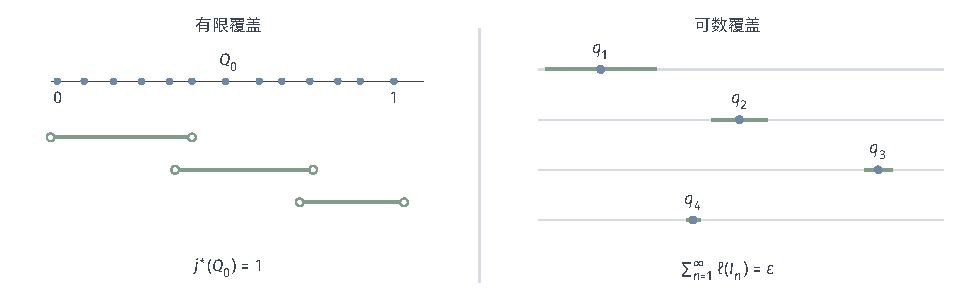
\includegraphics[width=169mm]{figures/01-mathematical-preliminaries-upper/01-mathematical-language-combinatorics-analysis-optimization/tikz/measure-countable-cover/figure.pdf}
 \caption{有限覆盖与可数覆盖。左侧画出一个有限开区间覆盖示例；对$Q_0=\mathbb Q\cap[0,1]$的任意有限区间覆盖，总长度均不小于$1$。右侧将一次完整覆盖改为可数个区间，图中取$\varepsilon=0.8$，只画列举中前四个点及其区间，长度依次为$\varepsilon2^{-n}$；使用全部区间时覆盖全部有理点，总长度为$\varepsilon$，并可随$\varepsilon$任意减小。点的有限示意不能表示有理点的完整稠密分布。}
 \label{fig:measure-countable-cover}
\end{figure*}

由此得到新的做法：允许用可数个区间组成一次完整覆盖，再用非负级数计算总长度。
实施这一做法需要第~\ref{sec:comb-countable-sets}节建立的列举与合并规则；下一小节从这些规则出发，定义新的外部长度估计。

\subsection{可数集与勒贝格外测度}
\label{sec:analysis-countable-outer-measure}

有限覆盖的限制已经说明了改变构造的理由：既要让每个可列举的点都分到自己的小区间，又要把所有区间的总长度控制住。
可数覆盖能同时做到这两件事，因为区间带有自然数编号，长度可以用已经学过的非负级数相加。

这一做法要用于后面的推导，还需要两项工具：可数个可数集合的并仍可数，保证合并若干组覆盖后仍是允许的覆盖；
非负双重级数可以合并，保证按组计算与统一编号计算得到同一个总长度。
这些工具建立后，就能定义勒贝格外测度，并检查它既能改进有理点集的估计，又保留普通区间的长度。

\subsubsection{可数覆盖的编号与长度}

第~\ref{sec:comb-countable-sets}节已定义可数集，并用对角列举证明自然数对、有理数与可数个可数集的并都可数。
因此$Q_0=\mathbb Q\cap[0,1]$可以列为$q_1,q_2,\ldots$，每个点都能分到自己的小区间；
合并一列可数覆盖时，所有区间也仍可统一编号。
余下要检查的是总长度：改变非负项的列举方式，不能改变覆盖长度的总和。

\paragraph{非负双重级数的合并}

沿用第~\ref{sec:analysis-continuous-limits}节对非负项级数规定的扩展总和，对$a_n\in[0,\infty]$有
\begin{equation}
 \sum_{n=1}^{\infty}a_n
 =\sup_{N\geq1}\sum_{n=1}^Na_n\in[0,\infty].
 \label{eq:comb-nonnegative-sum-supremum}
\end{equation}
非负性使有限和随加入新项而不减，所以也可以对所有有限索引集取上确界，结果相同。

对$a_{n,j}\geq0$，将双指标按任一无遗漏、无重复的顺序列成一个序列；由上一句，它的总和总是
\[
 S=\sup_{F\subseteq\mathbb N_+^2,\,F\text{有限}}
          \sum_{(n,j)\in F}a_{n,j},
\]
与所选顺序无关。下面证明$S=\sum_n\sum_j a_{n,j}$，即$S$等于先对每一行求和、再把各行之和相加的结果。

一方面，任取有限索引集$F$，它只涉及有限多行，并在每一行中只取有限多项；
每行取出的部分不超过该行之和，所以$\sum_{(n,j)\in F}a_{n,j}\leq\sum_n\sum_ja_{n,j}$。对$F$取上确界，得$S\leq\sum_n\sum_ja_{n,j}$。

另一方面，固定行数$N$与任意$\varepsilon>0$。若前$N$行之和都有限，对每个$n\leq N$选有限列数$J_n$，
使该行前$J_n$项之和超过整行之和减去$\varepsilon/N$。这些项组成一个有限索引集，所以
$S\geq\sum_{n=1}^N\sum_ja_{n,j}-\varepsilon$。令$\varepsilon\downarrow0$，再对$N$取上确界，得到$S\geq\sum_n\sum_ja_{n,j}$。
若某行之和为无穷，它的有限部分和可以超过任意给定的有限上界，同样迫使$S=+\infty$，此时两侧都为无穷。

这个证明只用到有限和与上确界的性质，因此这里的非负项换序不必借助后文的积分换序定理。

\subsubsection{勒贝格外测度}
\label{sec:comb-length-and-lebesgue-measure}

\paragraph{可数区间覆盖}

由于$Q_0$可以列为$q_1,q_2,\ldots$，逐点安排小区间的方案可以实施。
我们把这种覆盖方式用于一般集合：对$E\subseteq\mathbb R$，若有限或可数个有界开区间$I_j=(a_j,b_j)$满足$E\subseteq\bigcup_j I_j$，就称它们为$E$的可数区间覆盖。
区间可以重叠，也可以伸出$E$；它们的总长度为非负级数$\sum_j(b_j-a_j)$，允许等于$+\infty$。

“可数”限制的是覆盖区间的个数，不是$E$中的点数；一个开区间就可以覆盖含有不可数多个点的闭区间。
选择可数覆盖，是为了能逐项分配误差、用级数累计长度，并在合并覆盖时保留这两种能力。
前面没有给任意不可数族定义总长度，因此这里也不把“可数”放宽为不受限制的任意区间族。
采用开区间，则是为了在证明中使用闭区间的有限子覆盖性质；下面将用它保证原来的区间长度不被改变。

\paragraph{勒贝格外测度的定义}

一次覆盖可能伸出集合，也可能重复覆盖某些位置，所以它的总长度只是一个依赖于区间选择的外部估计。
为了尽量排除这些额外长度，我们对所有允许覆盖的总长度取下确界，得到勒贝格外测度。
\begin{definition}[勒贝格外测度]
\label{def:analysis-lebesgue-outer-measure}
对$E\subseteq\mathbb R$，定义其\term{勒贝格外测度}（Lebesgue outer measure）为
\begin{equation}
 m^*(E)=\inf\left\{\sum_{j=1}^{\infty}(b_j-a_j):
 \begin{array}{l}
 E\subseteq\bigcup_{j=1}^{\infty}(a_j,b_j),\\
 -\infty<a_j<b_j<\infty
 \end{array}\right\}.
 \label{eq:comb-lebesgue-outer-measure}
\end{equation}
这里也允许有限覆盖以及空集的空覆盖；空和为$0$。
\end{definition}

任意集合都能由覆盖整条实轴的一列区间覆盖，所以候选始终非空。
下确界可以为无穷，也不必由某个覆盖达到。
例如单点可以被任意短的开区间覆盖，其外测度为$0$；但任何覆盖都至少含一个非空开区间，总长度为正，所以没有覆盖能达到这个下确界。

\paragraph{空集与单调性}

空覆盖表明$m^*(\varnothing)=0$。
若$E\subseteq F$，任何覆盖$F$的区间族也覆盖$E$，
所以$F$的每个候选也是$E$的候选；在更大的候选集合上取下确界，结果不会更大，便得$m^*(E)\leq m^*(F)$。
这称为外测度的单调性，依据是两组候选覆盖之间的包含关系。

\paragraph{区间的外测度}

允许可数覆盖后，候选更多，下确界可能下降。我们希望有理点集的估计下降，但也必须检查普通区间的长度没有因此改变。
\begin{lemma}[区间的外测度等于长度]
\label{lem:set-measure-interval-outer-measure}
设$a<b$。对端点为$a,b$的有界区间$I$（两端可含可不含），有$m^*(I)=b-a$；无界区间的外测度为$+\infty$。
\end{lemma}
\begin{proof}
先证明$m^*([a,b])=b-a$。

上界：对任意$\varepsilon>0$，单个开区间$(a-\varepsilon/2,b+\varepsilon/2)$覆盖$[a,b]$，长度为$b-a+\varepsilon$。
令$\varepsilon\downarrow0$，得$m^*([a,b])\leq b-a$。

下界：这一侧必须控制每一种可数覆盖，不能只考察某一组区间。
任取$[a,b]$的可数开区间覆盖$\{(a_j,b_j)\}$。由闭区间的有限子覆盖性质（定理~\ref{thm:analysis-interval-finite-subcover}），其中有限个区间已经覆盖$[a,b]$；记它们的索引集为$F$。
初等集的有限覆盖不等式给出
\[
 b-a\leq\sum_{j\in F}(b_j-a_j)\leq\sum_{j=1}^{\infty}(b_j-a_j).
\]
对所有可数覆盖取下确界，得$m^*([a,b])\geq b-a$。

其他有界区间$I$包含长度任意接近$b-a$的闭区间，又有$I\subseteq[a,b]$，由单调性夹逼得$m^*(I)=b-a$。
无界区间包含任意长的有界闭区间，所以外测度为$+\infty$。
\end{proof}

所以改用可数覆盖后，区间的长度保持原值。

\paragraph{可数点集的外测度}

现在回到推动构造的例子，检验可数覆盖是否真正突破了有限覆盖的限制。
\begin{example}[可数点集的外测度为零]
\label{ex:set-measure-countable-outer-null}
设$E=\{x_1,x_2,\ldots\}$可数。任给$\varepsilon>0$，对每个$n$取
\[
 I_n=\bigl(x_n-\varepsilon2^{-n-1},\ x_n+\varepsilon2^{-n-1}\bigr).
\]
每个点$x_n$都落入$I_n$，所以这列区间覆盖全部$E$，且$\ell(I_n)=\varepsilon2^{-n}$。
于是
\[
 0\leq m^*(E)\leq\sum_{n=1}^{\infty}\varepsilon2^{-n}=\varepsilon.
\]
由于$\varepsilon$任意，$m^*(E)=0$。有限集只需用前有限个区间，同样得到外测度为$0$。
\end{example}

例中每个覆盖区间的长度都为正；趋于零的是整组覆盖的总长度上界，而不是一些未定义的正“无穷小”之和。

特别地，$m^*(Q_0)=0$，尽管$Q_0$的Jordan外容量为$1$。
有限覆盖的总长度不能低于$1$，可数覆盖却能把总长度压到任意给定的正数以内；改变的是一次完整覆盖所允许使用的区间族。
这与$m^*([0,1])=1$也不矛盾：$Q_0$可数，能够逐点编号；整个区间却不可数，无法给其中全部点各分配一个自然数编号，例中的覆盖方式不能用于$[0,1]$。

$m^*(Q_0)=0$回答的是外部估计能否下降的问题。
到这里，每个集合都已有外测度值，但还没有证明不交集合的外测度能够精确相加；要把外测度用于分块累计，还需要下面的可加性与可测性。

\subsubsection{可数可加性}

\paragraph{可数可加性的要求}

新的覆盖方式已经能累计可数个区间的长度，我们也希望测量规则能处理可数次不交分割。
例如，若一个可数点集作为各个单点的不交并参与精确相加，它的总长度就应等于单点长度之和。

一般地，对一个给集合赋值的映射$\nu$，希望有
\[
 \nu\left(\bigcup_{n=1}^{\infty}E_n\right)=\sum_{n=1}^{\infty}\nu(E_n),
 \qquad E_i\cap E_j=\varnothing\ (i\neq j),
\]
其中并集与各部分都应在$\nu$的赋值范围内。
这称为\term{可数可加性}（countable additivity），右侧是已经定义的非负项级数。

区间不可数，所以这一要求不允许把区间拆成全部单点后当作可数级数求和；
单点外测度为零与区间外测度为正并不矛盾。

\paragraph{外测度的可数次可加性}

已经建立的覆盖构造能先保证一个较弱的结论：把每个集合的覆盖合并，就得到并集的覆盖，
所以并集的外测度不超过各部分外测度之和。这只是不等式，并且不要求各集合不交。
这项性质称为\term{可数次可加性}（countable subadditivity）；名称中的“次”表示这里保证的是上界，不是精确相等。

每个集合未必有达到外测度的最优覆盖，证明时只能选近似最优覆盖。
因此需要把第$n$组的误差限制为$\varepsilon2^{-n}$，使合并无穷多组后总误差仍不超过$\varepsilon$。
\begin{theorem}[勒贝格外测度的可数次可加性]
\label{thm:analysis-outer-subadditivity}
对任意$E_1,E_2,\ldots\subseteq\mathbb R$，有
\begin{equation}
 m^*\left(\bigcup_{n=1}^{\infty}E_n\right)
 \leq\sum_{n=1}^{\infty}m^*(E_n).
 \label{eq:analysis-outer-subadditivity}
\end{equation}
\end{theorem}
\begin{proof}
若右侧为$+\infty$，不等式直接成立。
设右侧有限，则每个$m^*(E_n)$有限。给定$\varepsilon>0$，由下确界定义，
为每个$E_n$选择覆盖$\{I_{n,j}:j\geq1\}$，使
\[
 E_n\subseteq\bigcup_j I_{n,j},\qquad
 \sum_j\ell(I_{n,j})<m^*(E_n)+\varepsilon2^{-n}.
\]
空集可以取空覆盖，有限覆盖直接作为有限组处理。
所有$I_{n,j}$覆盖$\bigcup_nE_n$；可数个可数集的并仍可数，故它们是允许使用的一组覆盖。
再由非负双重级数的合并规则，
\[
 \begin{aligned}
 m^*\left(\bigcup_nE_n\right)
 &\leq\sum_{n,j}\ell(I_{n,j})\\
 &=\sum_n\sum_j\ell(I_{n,j})
 \leq\sum_nm^*(E_n)+\varepsilon.
 \end{aligned}
\]
最后让$\varepsilon\downarrow0$，得到所需不等式。
\end{proof}

\paragraph{一般外测度}

刚才的证明只给出不等式，尚未要求不交集合的值精确相加。
空集取值为零、单调性与可数次可加性这三条性质不依赖区间长度的具体形式；把它们抽取出来，便得到可用于其他测量构造的一般概念。
\begin{definition}[外测度]
\label{def:analysis-outer-measure}
集合$X$上的映射$\mu^*:\mathcal P(X)\to[0,\infty]$，若满足
\[
 \begin{gathered}
 \mu^*(\varnothing)=0,\\
 A\subseteq B\Longrightarrow\mu^*(A)\leq\mu^*(B),\\
 \mu^*\left(\bigcup_{n=1}^{\infty}E_n\right)\leq\sum_{n=1}^{\infty}\mu^*(E_n)
 \quad(E_n\subseteq X),
 \end{gathered}
\]
则称为\term{外测度}（outer measure）。
\end{definition}
前面已经证明勒贝格外测度满足这三条，所以它是外测度的一个实例；其中第三条来自覆盖的合并，而覆盖合并没有给出反向不等式。
即使$E_n$两两不交，分别覆盖它们的开区间也可能彼此重叠；集合不交并不会使覆盖的长度自动精确相加。
反过来，把覆盖并集的区间按任意集合切开，所得部分又未必是区间，不能直接沿用区间长度公式来分配总量。
因此，不能仅凭这三个条件便把式~\eqref{eq:analysis-outer-subadditivity}中的不等号改为等号。

下一步要补上的，是集合与这套外部估计之间的分割相容性：用一个集合切分任意测试集，切分后两部分的外测度之和仍等于原值。
我们将把满足这个要求的集合选出来，再证明在它们组成的范围内，不交可数并确实能够精确相加。

\subsection{可测集与勒贝格测度}
\label{sec:analysis-lebesgue-measurable-construction}

现在需要区分两个问题：一个集合能否取得外测度值，以及它能否在分割计算中保持精确相加。
第一个问题已经解决，任意集合都有$m^*$值；第二个问题还没有由覆盖构造保证。
要为积分准备可以反复分块的测量规则，就需要找出能够保持精确分割的集合，这就是引入可测集的原因。

下面保留原来的$m^*$数值，要求一个集合用来切分任何测试集时，都不改变分割前后的总量。
我们先写出这个条件，再证明满足条件的集合对取补和可数并封闭，最后证明限制到这一范围的$m^*$具有可数可加性。

\subsubsection{可测性的要求}

\paragraph{精确分割}

固定一个待检验的集合$A$，再任取测试集$E$。$A$把$E$分成落在$A$内的部分和落在$A$外的部分：
\[
 E=(E\cap A)\cup(E\setminus A),\qquad
 (E\cap A)\cap(E\setminus A)=\varnothing.
\]
次可加性已经保证$m^*(E)\leq m^*(E\cap A)+m^*(E\setminus A)$。
若要分割不改变总量，还需要反向不等式；缺少它时，两部分分别作外部估计，所得总和可能比整体的外部估计大。

外测度的三条公理确实不能自动排除这种情况，下面的两点空间就是一个有限例子。
\begin{example}[两点空间上不可加的外测度]
\label{ex:set-measure-two-point-outer-measure}
在两点集合$X=\{a,b\}$上，令$\mu^*(\varnothing)=0$，并令每个非空子集的值都为$1$。

单调性：若$A\subseteq B$且$A$非空，则$B$也非空，两者的值都为$1$；若$A$为空集，则$\mu^*(A)=0\leq\mu^*(B)$。

可数次可加性：若一列子集的并为空，各项都是空集，两侧均为$0$；若并非空，至少有一项非空，右侧至少为$1$，不小于左侧的$1$。

所以$\mu^*$是外测度。但取$E=X$、$A=\{a\}$时，
\[
 1=\mu^*(X)<\mu^*(\{a\})+\mu^*(\{b\})=2,
\]
即集合$\{a\}$不能精确分割测试集$X$。
\end{example}

这个例子只说明仅有三条公理不足以推出精确相加，并不是勒贝格外测度下的不可测集构造。
图~\ref{fig:measure-exact-splitting}把它与区间的精确分割放在一起，展示可测性条件要排除的总量变化。

\begin{figure*}[htbp]
 \centering
 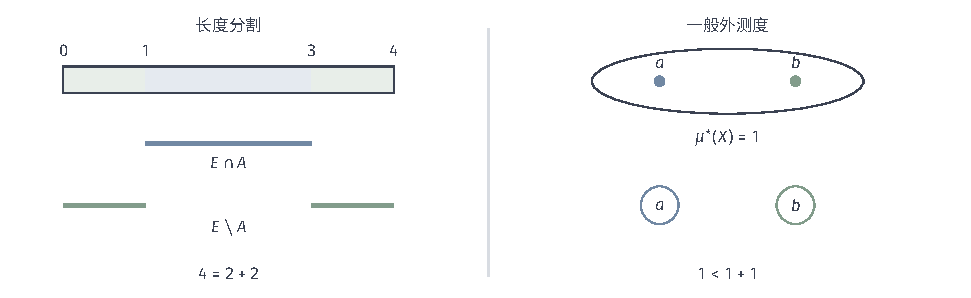
\includegraphics[width=169mm]{figures/01-mathematical-preliminaries-upper/01-mathematical-language-combinatorics-analysis-optimization/tikz/measure-exact-splitting/figure.pdf}
 \caption{精确分割与一般外测度的差别。左侧用$A=[1,3]$分割测试集$E=[0,4]$，落在$A$内的长度为$2$，外部两段总长度也为$2$，两者恢复原来的$4$；有限端点不改变长度。右侧使用正文两点空间的外测度，整体值为$1$，拆成两个单点后的值之和为$2$。右侧并非勒贝格不可测集的图像；左侧也只画了一个测试集，可测性定义要求对每个测试集都有精确等式。}
 \label{fig:measure-exact-splitting}
\end{figure*}

勒贝格外测度也存在不能保持精确分割的集合；这类不可测集的存在与构造可参考测度论教材\scite{math-hunter2011measure,math-folland1999real}，这里不展开。
下面直接以精确分割为条件选取可测集，并证明这类集合上的可加性。

\paragraph{可测集的定义}

我们希望$A$能够在不同范围的计算中反复参与分割，因此条件不能只针对某个预先选好的$E$，而要对所有测试集成立。
满足这一要求的$A$称为勒贝格可测集。
\begin{definition}[勒贝格可测集]
\label{def:analysis-lebesgue-measurable-set}
集合$A\subseteq\mathbb R$称为\term{勒贝格可测集}（Lebesgue measurable set），若对每个$E\subseteq\mathbb R$都有
\begin{equation}
 m^*(E)=m^*(E\cap A)+m^*(E\setminus A).
 \label{eq:comb-caratheodory-measurability}
\end{equation}
全体勒贝格可测集组成的集合族记为$\mathcal L(\mathbb R)$。
\end{definition}

式~\eqref{eq:comb-caratheodory-measurability}称为Carathéodory可测性条件。
由于$m^*(E)\leq m^*(E\cap A)+m^*(E\setminus A)$已由次可加性保证，验证可测性只需证明
$m^*(E)\geq m^*(E\cap A)+m^*(E\setminus A)$。
条件必须对每个$E$检验：只令$E=A$得到的是$m^*(A)=m^*(A)+m^*(\varnothing)$，对任意集合都成立，无法区分哪些分割与外测度相容。
“可测”并不表示此前无法给$A$求值；$m^*(A)$对任意$A$都已定义，新增的要求是$A$与所有测试集的分割相容。

外测度为零的集合不需要逐个验证分割；下面的引理一次处理所有这样的集合及其子集，以后处理零测余量和完备性时都会用到。
\begin{lemma}[零外测度集的子集可测]
\label{lem:analysis-zero-outer-measure-measurable}
若$N\subseteq\mathbb R$且$m^*(N)=0$，则每个$D\subseteq N$都勒贝格可测，并且$m^*(D)=0$。
\end{lemma}
\begin{proof}
单调性先给出$m^*(D)=0$。对任意测试集$E$，有
\[
 m^*(E\cap D)+m^*(E\setminus D)=0+m^*(E\setminus D)\leq m^*(E).
\]
结合外测度次可加性给出的反向不等式，得到可测性所需的精确分割等式。
\end{proof}

由示例~\ref{ex:set-measure-countable-outer-null}，$m^*(Q_0)=0$，所以此引理立即说明$Q_0$勒贝格可测。
利用$Q_0$的可测性，还可以算出$[0,1]$中无理点集的外测度。
\begin{example}[单位区间中无理点的外测度]
\label{ex:set-measure-irrationals-outer-measure}
在$Q_0$的可测性条件中取测试集$E=[0,1]$。由于$E\cap Q_0=Q_0$、$E\setminus Q_0=[0,1]\setminus Q_0$，得到
\[
 1=m^*([0,1])=m^*(Q_0)+m^*([0,1]\setminus Q_0)=0+m^*([0,1]\setminus Q_0).
\]
所以$[0,1]$中无理点组成的集合外测度为$1$。
\end{example}

有理点与无理点都分布在$[0,1]$的每一小段中，却不因此占有相同的长度。
可测性由分割等式判断，而不是由集合看起来是否稠密、光滑或规则判断。

\subsubsection{可测集族}

前面的定义逐个检验一个集合能否精确切分任意测试集。接下来还要检验：可测集经过取补、合并等运算后，是否仍然可测？

如果每次分块或合并都可能离开允许测量的范围，就无法反复使用这套测量方法。
Jordan测量就有这个问题：每个单点$\{q_n\}$都Jordan可测，它们的可数并$Q_0$却不Jordan可测（示例~\ref{ex:set-measure-rationals-not-jordan}）。
可见，每个部分都能参与测量，还不能保证合并后的对象也能参与测量。

勒贝格构造需要解决这个范围问题：先证明可测集族对所需运算封闭，再讨论合并后数值怎样相加。

\paragraph{取补与有限并}

取补对应保留分割的另一侧，有限并对应把有限块合为一块；先检查这两类操作，便能处理有限次分块计算。
下面始终用任意测试集$E$检验所得集合，并以已经证明的次可加性作为其中一个方向。

空集满足$m^*(E)=0+m^*(E)$，所以可测。
把$A$换成$\mathbb R\setminus A$只交换式~\eqref{eq:comb-caratheodory-measurability}右边的两项，因此取补保持可测，特别地$\mathbb R$也可测。

若$A,B$可测，先用$A$分割$E$，再用$B$分割$E\setminus A$，得到
\[
 \begin{aligned}
 m^*(E)&=m^*(E\cap A)+m^*((E\setminus A)\cap B)\\
 &\quad +m^*(E\setminus(A\cup B))\\
 &\geq m^*(E\cap(A\cup B))+m^*(E\setminus(A\cup B)).
 \end{aligned}
\]
前两部分恰好组成$E\cap(A\cup B)$，次可加性使它们的外测度之和不小于这个并的外测度，这就给出最后一行的不等式。
结合次可加性给出的另一方向，每个$E$都满足精确分割，所以$A\cup B$可测。
再由$A\cap B=(A^c\cup B^c)^c$和$A\setminus B=A\cap B^c$，得到有限交与差的可测性，这里的补集均相对于$\mathbb R$。

若$A,B$还不交，用$A$分割测试集$E\cap(A\cup B)$，又得到
\[
 m^*(E\cap(A\cup B))=m^*(E\cap A)+m^*(E\cap B).
\]
反复应用即可处理任意有限个两两不交的可测集。
这里同时得到了两件事：有限并仍在可测范围内；对不交的有限部分，切分前后的外测度精确相加。
后面处理可数并时，将从这两条有限结论出发，不预先假定无限情形已经成立。

\paragraph{可数并}

有限次合并不会离开可测范围，但一列集合的并不能在有限步内完成，所以可数并的可测性需要单独证明。
证明的办法是先精确切出前$N$块，再让非负部分和随$N$增加，而不直接调用尚未建立的测度可数可加性。

先设$C_n$两两不交且可测，令$U_N=\bigcup_{n=1}^NC_n$、$U=\bigcup_{n=1}^{\infty}C_n$。
对每个测试集$E$和每个$N$，先用可测集$U_N$分割$E$，再对$E\cap U_N$反复使用不交有限部分的等式，得到下式中的等号；
又因为$E\setminus U\subseteq E\setminus U_N$，外测度的单调性给出不等号：
\[
 \begin{aligned}
 m^*(E)
 &=\sum_{n=1}^Nm^*(E\cap C_n)+m^*(E\setminus U_N)\\
 &\geq\sum_{n=1}^Nm^*(E\cap C_n)+m^*(E\setminus U).
 \end{aligned}
\]
左侧不依赖$N$，令$N\to\infty$，非负部分和递增到级数之和，得到整列分割的下界；再用外测度的可数次可加性合并各个$E\cap C_n$，得到
\[
 m^*(E)\geq\sum_{n=1}^{\infty}m^*(E\cap C_n)+m^*(E\setminus U)
 \geq m^*(E\cap U)+m^*(E\setminus U).
\]
这就是$U$的可测性条件，故不交可测集的可数并可测。

若$A_n$不一定不交，令$C_1=A_1$、$C_n=A_n\setminus\bigcup_{j<n}A_j$。
每个$C_n$只用有限并与差集构成，所以已知可测；逐项去掉此前出现的部分，又使它们两两不交且并集不变。
对$C_n$应用刚才的结论，就证明了一般可数并仍可测。
至此，取补、有限并和可数并都不会使我们离开$\mathcal L(\mathbb R)$。

\paragraph{$\sigma$代数}

刚才证明的封闭性质，正是后续反复分块和合并时需要的范围保证。
为了在其他对象集合上也使用同样的保证，下面把“包含全集、取补封闭、可数并封闭”统一定义为$\sigma$代数。
\begin{definition}[$\sigma$代数]
\label{def:analysis-sigma-algebra}
设$X$为集合。若子集族$\mathcal A\subseteq\mathcal P(X)$满足
\[
 \begin{gathered}
 X\in\mathcal A,\\
 A\in\mathcal A\Longrightarrow X\setminus A\in\mathcal A,\\
 A_1,A_2,\ldots\in\mathcal A
 \Longrightarrow\bigcup_{n=1}^{\infty}A_n\in\mathcal A,
 \end{gathered}
\]
则称$\mathcal A$为$X$上的\term{$\sigma$代数}（sigma-algebra）。
\end{definition}

由取补可得$\varnothing\in\mathcal A$；在有限个集合之后补上无穷多个空集，便由可数并得到有限并。
De Morgan公式又给出可数交：$\bigcap_nA_n=X\setminus\bigcup_n(X\setminus A_n)$。
可数交在构造中经常出现：例如$\{a\}=\bigcap_{n\geq1}(a-1/n,a+1/n)$，单点就是一列开区间的交。
只对有限运算封闭的集合族不能保证这类由无限过程得到的集合仍在范围内，$\sigma$代数则把可数运算也纳入同一个范围。

在当前的勒贝格构造中，$\mathcal L(\mathbb R)$先由精确分割条件选出，再由前面的推导证明是$\sigma$代数；
我们没有预先假定所有可测集合自动具有这些封闭性。
在抽象测量问题中，则可以先指定一个$\sigma$代数来规定允许测量的范围。
两种做法的起点不同，但得到的范围具有相同的结构。

$\sigma$代数记录允许测量的子集，并保证这些子集经过所需的集合运算后仍在这一范围内；它没有给集合赋予大小，也没有单独保证任何数值的可加性。
所以接下来还要把已经构造的外测度放到这个可测范围上，证明它确实满足精确相加的规则。

\subsubsection{勒贝格测度}

\paragraph{限制外测度}

现在有了两个对象：$m^*$负责给集合赋值，$\mathcal L(\mathbb R)$负责保证取补和可数合并后仍在可测范围内。
我们保留$m^*$在可测集上的原值，把允许的输入从所有子集收缩为$\mathcal L(\mathbb R)$，并给这个限制后的赋值命名。
\begin{definition}[勒贝格测度]
\label{def:analysis-lebesgue-measure}
勒贝格外测度在$\mathcal L(\mathbb R)$上的限制
\[
 m:\mathcal L(\mathbb R)\to[0,\infty],\qquad m(A)=m^*(A),
\]
称为\term{勒贝格测度}（Lebesgue measure）。
\end{definition}

这一步没有重新计算任何可测集的大小：例如$m(Q_0)=m^*(Q_0)=0$，空集仍有$m(\varnothing)=0$。
改变的只是赋值的定义域；$m$在这个定义域上是否可数可加，还需要下面证明。

\paragraph{不交可测并的可数可加性}

$\sigma$代数已经保证可数并是允许的输入，因此等式左侧有定义；精确分割条件则使每个有限不交部分和都成为并集测量值的下界。
对这些下界取上确界，再结合外测度原有的次可加上界，就能把不等式收紧为等式。
\begin{theorem}[勒贝格测度的可数可加性]
\label{thm:analysis-lebesgue-countable-additivity}
若$A_n\in\mathcal L(\mathbb R)$两两不交，则
\[
 m\left(\bigcup_{n=1}^{\infty}A_n\right)=\sum_{n=1}^{\infty}m(A_n).
\]
\end{theorem}
\begin{proof}
记$A=\bigcup_n A_n$。前面已证明$A$可测；对每个$N$，由单调性与有限分割，
\[
 m(A)\geq m\left(\bigcup_{n=1}^NA_n\right)=\sum_{n=1}^Nm(A_n).
\]
对$N$取上确界，得到$m(A)\geq\sum_n m(A_n)$。
反向不等式正是外测度的可数次可加性，因为$m$与$m^*$在这些集合上相同。
\end{proof}

因此，从$m^*$到$m$经过了两个相接的步骤：先由精确分割条件选出$\mathcal L(\mathbb R)$，并证明它对可数并封闭，保证合并后的集合仍可测量；
再证明保留在这一范围上的数值可数可加，保证合并后集合的测量值等于不交部分之和。
这两步共同使勒贝格测度能够用于反复的分块累计。

类似构造也适用于一般外测度；这里只给出一维长度所需的关键封闭性与可加性步骤，
更一般的表述在第~\ref{chap:measure-spaces}章建立，也可参考测度论教材\scite{math-hunter2011measure,math-folland1999real}。

\paragraph{区间与常见可测集}

可数可加性定理只适用于已经可测的集合，所以还要确认普通区间、开集等常用对象确实属于$\mathcal L(\mathbb R)$。
先从半直线开始：它只在一个位置切分区间，容易把可测性条件还原为已知的长度之和。

固定$t\in\mathbb R$，考虑半直线$H=(-\infty,t]$。
若$m^*(E)<\infty$，给定$\varepsilon>0$，选择总长度小于$m^*(E)+\varepsilon$的开区间覆盖$\{I_j\}$。
将每个$I_j$在$t$处切成$I_j\cap H$与$I_j\setminus H$两段；两段可能是开区间、半开区间或空集，
由引理~\ref{lem:set-measure-interval-outer-measure}，它们的外测度等于各自长度，而两段长度之和仍是$\ell(I_j)$。
两组小段分别覆盖$E\cap H$和$E\setminus H$，由外测度的次可加性得
\[
 \begin{aligned}
 &m^*(E\cap H)+m^*(E\setminus H)\\
 &\quad\leq\sum_j\bigl[m^*(I_j\cap H)+m^*(I_j\setminus H)\bigr]\\
 &\quad=\sum_j\ell(I_j)<m^*(E)+\varepsilon.
 \end{aligned}
\]
令$\varepsilon\downarrow0$就得到所需的反向不等式。
若$m^*(E)=\infty$，次可加性已迫使分割后的总和也为无穷，等式自动成立。
所以$H$可测。

半直线的差给出半开区间；再取可数并与可数交，就得到其他端点型式的区间和单点。
任意开集是其中所有有理端点开区间的并：对开集中的每个点，先取完全落在开集内的小区间，再利用有理数的稠密性缩小端点，使端点为有理数而区间仍含该点。
有理端点对可数，所以这是一组可数并；于是开集、其补集以及再经可数集合运算所得的集合都可测。
区间长度结论也随之保留为
\[
 m((a,b))=m([a,b])=m([a,b))=b-a,\qquad m(\{a\})=0.
\]

\paragraph{Borel集合}

区间与开集已经可测，但以后往往从它们出发反复取补、作可数并或可数交。
为了统一指明这些操作必然产生的集合，下面定义包含全部开区间的最小$\sigma$代数。

这样的最小范围确实存在：$\mathcal P(\mathbb R)$是一个包含所有开区间的$\sigma$代数，故候选不空。
把全部候选取交，所得集合族仍包含全集；对它的成员取补或作可数并，结果仍属于每个候选，所以交族本身也是$\sigma$代数。
它包含所有开区间，又包含于每个候选，因而正是所需的最小范围，称为由开区间生成的$\sigma$代数。
\begin{definition}[Borel $\sigma$代数]
\label{def:analysis-borel-sigma-algebra}
实轴上由所有开区间$(a,b)$（$a<b$）生成的最小$\sigma$代数记为$\mathcal B(\mathbb R)$，称为\term{Borel $\sigma$代数}（Borel sigma-algebra）。
对$X\subseteq\mathbb R$，令
\[
 \mathcal B(X)=\{X\cap B:B\in\mathcal B(\mathbb R)\},
\]
称为$X$上的Borel $\sigma$代数；其中的集合称为Borel集合。
\end{definition}

由前面对开集的表示，$\mathcal B(\mathbb R)$也等于所有开集生成的$\sigma$代数。
例如$\{a\}=\bigcap_{n\geq1}(a-1/n,a+1/n)$是Borel集合，可数点集作为可数个单点的并也是Borel集合。
各范围之间有
\[
 \mathcal B(\mathbb R)\subseteq\mathcal L(\mathbb R)\subseteq\mathcal P(\mathbb R),
 \qquad m=m^*\big|_{\mathcal L(\mathbb R)}.
\]
第一个包含关系来自可测范围的封闭性：$\mathcal L(\mathbb R)$已经是包含所有开区间的$\sigma$代数，必包含最小的$\mathcal B(\mathbb R)$。
第二个包含关系只说明可测集也是实轴子集，并不表示全部子集都可测；前面已经指出勒贝格外测度下存在不可测集，其构造不在这里展开。
这里$\mathcal B(\mathbb R)$与$\mathcal L(\mathbb R)$都是集合族，规定允许的范围；$m$与$m^*$是给集合赋值的函数，职责不同。

\paragraph{Jordan测量与勒贝格测度}

前面已经说明区间长度保持不变，现在进一步检验：每个Jordan可测集是否都勒贝格可测，且两种测量值相同。
证明中的零测余量由引理~\ref{lem:analysis-zero-outer-measure-measurable}处理：外测度为零的集合的任意子集都已可测，因此内部Borel部分之外的零测误差不会破坏可测性。

若$E$为Jordan可测集，对每个$n$取初等集$A_n\subseteq E\subseteq B_n$，
使$\ell(B_n)-\ell(A_n)<2^{-n}$。
令$A=\bigcup_nA_n$、$B=\bigcap_nB_n$，则$A,B$均为Borel集合，且$A\subseteq E\subseteq B$。
由于$B\setminus A\subseteq B_n\setminus A_n$，而在初等集上$m$与$\ell$相同，有
$m(B\setminus A)\leq\ell(B_n)-\ell(A_n)<2^{-n}$对所有$n$成立，故$m(B\setminus A)=0$。
$E\setminus A$包含于$B\setminus A$，由该引理可测，于是$E=A\cup(E\setminus A)$也可测。

最后比较数值。任一内部候选$A'\subseteq E$与外部候选$B'\supseteq E$都满足$\ell(A')=m(A')\leq m(E)\leq m(B')=\ell(B')$，
分别取上确界与下确界得$j_*(E)\leq m(E)\leq j^*(E)$，从而$m(E)=j(E)$。

因此Jordan可测集都勒贝格可测，数值保持一致；$Q_0$则说明逆向不成立：它在每个小区间中都稠密，不Jordan可测，却是可数Borel集合，勒贝格测度为零。

\subsection{勒贝格测度的性质}
\label{sec:comb-measurable-sets-and-weights}

勒贝格测度已经在可测集族$\mathcal L(\mathbb R)$上定义，并满足可数可加性。
积分要按可测集合的大小累计函数取值，计算中还会遇到包含、重叠以及逐步扩大或缩小的集合；
函数也可能只在长度为零的范围内取不同值。下面只就实轴上的勒贝格测度$m$，推导后面积分要用到的三组性质：
由不交分割得到的大小比较与集合列极限，零测集与几乎处处的例外语言，以及康托尔集与康托尔函数，前者说明零测集可以不可数，后者的全部增长集中在一个零测集上。
把这些结构推广到一般集合上的测度空间，留给第~\ref{chap:measure-spaces}章。

\subsubsection{基本性质与集合列}
\label{sec:comb-set-approximation}
\label{sec:analysis-set-measure-continuity}

可数可加性只直接规定了不交可数并的测度。包含、重叠和嵌套的集合关系都要先改写成不交分割，才能使用这一规则。
下面先由分割得到大小比较和重叠集合的上界，再研究一列集合的并、交与测量值极限的关系。
以下集合均属于$\mathcal L(\mathbb R)$；推导只用到可数可加性与可测集族对取补、可数并的封闭性。

\paragraph{单调性}

若$A\subseteq B$，较大的集合只比$A$多出$B\setminus A$这一部分。对可测的$A,B$，差集也可测，且$A$与$B\setminus A$不交，因此
\[
 m(B)=m(A)+m(B\setminus A)\geq m(A).
\]
这称为测度的单调性：包含关系给出测量值的大小比较。

若$m(B)<\infty$，还可以写成$m(B\setminus A)=m(B)-m(A)$，用总量减去已知部分计算余量。
这里的有限性不能省略：可加等式允许无穷值，相减却不能出现$\infty-\infty$。
例如$A=(0,\infty)$、$B=\mathbb R$时两者的测度都为无穷，差集$(-\infty,0]$的测度不能由相减得到。

\paragraph{次可加性}

集合有重叠时，直接相加会重复计算。对可测集合列$A_n$，把每一步已经出现的部分去掉，令
\[
 B_1=A_1,\qquad B_n=A_n\setminus\bigcup_{j<n}A_j\quad(n\geq2).
\]
$B_n$仍可测、两两不交，且与原集合列有相同的并；又有$B_n\subseteq A_n$，故
\[
 m\left(\bigcup_nA_n\right)=\sum_nm(B_n)\leq\sum_nm(A_n).
\]
这就是可数次可加性：即使各部分有重叠，也能用各部分测度之和控制并集的测度。
它还说明可数个零测集的并仍是零测集，因为此时右侧为$0$；后面合并例外范围时会用到这一点。

若$A,B$的测度有限，还可以精确校正重复部分。把$A\cup B$分成两两不交的$A\setminus B$、$A\cap B$与$B\setminus A$，由可加性有
\[
 m(A)=m(A\setminus B)+m(A\cap B),\qquad m(B)=m(B\setminus A)+m(A\cap B),
\]
而$m(A\cup B)$等于三部分测度之和。前两式相加后减去一份$m(A\cap B)$，得到
\[
 m(A\cup B)=m(A)+m(B)-m(A\cap B).
\]
这是测度形式的容斥公式；有限性保证其中的减法有意义。
例如$A=[0,2]$、$B=[1,3]$时，右侧为$2+2-1=3$，正是$A\cup B=[0,3]$的长度。

\paragraph{递增集合列}

有时一个范围是逐步加入新部分形成的，例如用越来越多的区间逼近一个开集。此时要知道，每一步的测量值能否确定最终并集的测量值。
若$A_1\subseteq A_2\subseteq\cdots$且$A=\bigcup_nA_n$，记为$A_n\uparrow A$。
可测范围对可数并封闭，所以$A$可测；下面说明测量值也能取极限。

增量$B_1=A_1$、$B_n=A_n\setminus A_{n-1}$两两不交，且
$A_n=\bigcup_{j=1}^nB_j$、$A=\bigcup_{j=1}^{\infty}B_j$。
于是可数可加性把集合的逐步增加转成非负部分和的逐步增加：$m(A_n)=\sum_{j=1}^nm(B_j)$，$m(A)=\sum_{j=1}^{\infty}m(B_j)$，得到
\begin{equation}
 m(A)=\sup_{n\geq1}m(A_n)=\lim_{n\to\infty}m(A_n).
 \label{eq:comb-measure-continuity-below}
\end{equation}
这个结论称为测度的下连续性，不要求$m(A)$有限；非负部分和的极限也可以是$+\infty$。
例如$A_n=(0,1-1/n)$递增，并集为$(0,1)$，各步长度$1-1/n$趋于$1$，正好等于并集的长度。

\paragraph{递减集合列}

逐步去掉部分时，最终留下的是交集。若$A_1\supseteq A_2\supseteq\cdots$且$A=\bigcap_nA_n$，记为$A_n\downarrow A$。
交集可测，但要由各步测度恢复交集测度，还需要一个有限总量作为相减的起点。

设$m(A_1)<\infty$。把留下的范围改为已经去掉的范围，$A_1\setminus A_n$便递增到$A_1\setminus A$。
对它应用下连续性，再利用所有集合都包含在有限测度的$A_1$中，把差集的测度写成相减，得到
\[
 m(A_1)-m(A)=\lim_{n\to\infty}\bigl[m(A_1)-m(A_n)\bigr].
\]
所有减法都在有限数值之间进行，整理后有
\begin{equation}
 m(A)=\inf_{n\geq1}m(A_n)=\lim_{n\to\infty}m(A_n).
 \label{eq:comb-measure-continuity-above}
\end{equation}
这称为测度的上连续性。若只知道某个$A_{n_0}$的测度有限，舍去它之前的有限项后，也能应用同一结论。

例如$[0,1/n]\downarrow\{0\}$，长度$1/n$递减趋于$0=m(\{0\})$。
有限性条件确有作用，去掉它以后结论可能失效。
\begin{example}[测度无穷时上连续性失效]
\label{ex:set-measure-continuity-above-failure}
考虑区间列$(n,\infty)$，$n\geq1$。它们逐项递减；任意实数$x$在$n>x$时都不属于$(n,\infty)$，所以这些区间的交为空集。
每一项都包含任意长的有界区间，测度均为$+\infty$，于是
\[
 \lim_{n\to\infty}m((n,\infty))=+\infty\neq0=m(\varnothing).
\]
\end{example}

各项的测度只记录了总量为无穷，没有反映这些集合正在向右移走，所以不能由各项测度的下确界得到交集的测度。
图~\ref{fig:vol1-add-nested-set-limits}对照递增、有限测度下递减及缺少有限性时失败的三种情形。
\begin{figure}[!htb]
  \centering
  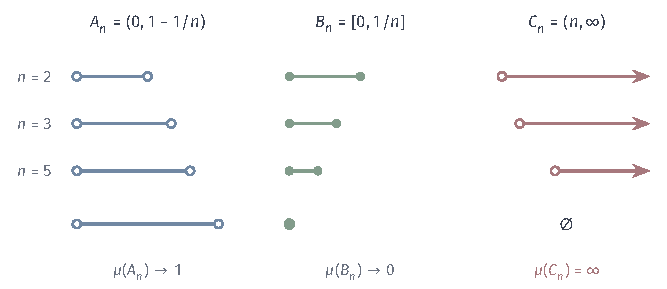
\includegraphics[width=112mm]{figures/01-mathematical-preliminaries-upper/01-mathematical-language-combinatorics-analysis-optimization/tikz/comprehension-additions/nested-set-limits.pdf}
  \caption{实轴上的三列嵌套集合，依次画$n=2,3,5$及最终的并集或交集，均使用勒贝格测度。左列$A_n$递增，并集为$(0,1)$；中列$B_n$递减，交集为$\{0\}$；右列$C_n=(n,\infty)$递减，交集为空，而每一项的测度仍为无穷。空心、实心端点分别表示不包含、包含；各列仅在本列内共用坐标尺度。}
  \label{fig:vol1-add-nested-set-limits}
\end{figure}
\FloatBarrier

\subsubsection{零测集与几乎处处}
\label{sec:comb-null-sets-and-completion}

集合差的测度可以描述遗漏或多出的总量。当这份总量恰为零时，函数仍可能在其中某些点取不同值，某个性质也可能在那里失效。
我们需要说明什么是零测范围、怎样表达一个性质只在零测范围内有例外，以及零测范围究竟能包含多少点。
前两个问题引出零测集和几乎处处，最后一个问题由康托尔集回答；同一删除过程还给出康托尔函数，它的增长全部集中在一个零测集上。

\paragraph{零测集}

测度为零不等于没有元素：勒贝格测度给单点赋值$0$，点本身却仍然存在。
为了用测量值而非点数描述这种范围，先给它一个名称。
\begin{definition}[零测集]
\label{def:analysis-null-set-almost-everywhere}
若$N\in\mathcal L(\mathbb R)$且$m(N)=0$，称$N$为（勒贝格）\term{零测集}（null set）。
\end{definition}
单点与所有可数点集都是零测集：它们是Borel集合，因而可测；由可数次可加性，它们的测度又不超过各单点测度之和$0$。
零测集的任意子集也是零测集：引理~\ref{lem:analysis-zero-outer-measure-measurable}已经证明，外测度为零的集合的子集都可测，单调性又使其测度为零。
因此讨论例外范围时，只要它包含在某个零测集中，就不必再单独验证它的可测性；勒贝格测度的这一性质称为完备性。

\paragraph{几乎处处}

比较两个函数时，除了判断它们是否逐点相等，还可以考察它们取值不同的位置是否都落在一个零测集中。
一般性质的例外范围也用同样的方式描述。
\begin{definition}[几乎处处]
设$E\in\mathcal L(\mathbb R)$。若存在零测集$N$，使某性质对每个$x\in E\setminus N$成立，称该性质在$E$上\term{几乎处处}（almost everywhere，简写为a.e.）成立。
\end{definition}
例如$f(0)=1$、$f(x)=0$（$x\neq0$）与恒零函数几乎处处相等，尽管它们在$0$处并不相等。
例外范围也可以是无限集，并且出现在每一小段中。
\begin{example}[有理点指示函数几乎处处为零]
在$[0,1]$上考虑$f=\mathbb I_{Q_0}$，即$x\in Q_0$时$f(x)=1$，否则$f(x)=0$。
$f$与恒零函数取值不同的点恰好组成$Q_0$，而$m(Q_0)=0$，所以$f=0$在$[0,1]$上几乎处处成立。

再看连续性。$[0,1]$中每个点的任意邻域与$[0,1]$的交都含正长度区间，因而既含$Q_0$中的点，也含无理点；$f$在其中同时取到$1$和$0$，所以$f$在$[0,1]$上处处不连续。
恒零函数则处处连续。
\end{example}

这个例子说明，“几乎处处”不表示只遗漏有限个点，也不表示每个位置附近都没有例外；几乎处处相等也不会自动保留连续性或某个指定点的取值。
后面讨论积分时，会明确哪些结论只依赖零测范围之外的取值。

若一列性质分别在零测集$N_1,N_2,\ldots$之外成立，那么它们在$\bigcup_nN_n$之外同时成立，而这个并仍是零测集。
所以可数多项几乎处处结论可以使用共同的例外范围。这一做法不能推广到不可数多项结论。
\begin{example}[不可数多项几乎处处结论不能合并]
在$[0,1]$上，对每个$t\in[0,1]$考虑性质$P_t$：$x\neq t$。它只在单点$t$处失效，所以每个$P_t$都在$[0,1]$上几乎处处成立。
若要求全部$P_t$同时成立，例外范围是$\bigcup_{t\in[0,1]}\{t\}=[0,1]$，测度为$1$；也就是说，没有任何$x\in[0,1]$满足所有$P_t$。
\end{example}

这里的并有不可数多项，可数次可加性不再适用。

\paragraph{康托尔集}
\label{sec:analysis-cantor-set}

可数集是熟悉的零测集，但零测是否意味着最多只有可数多个点，还需另行检验。
下面的康托尔集说明，点的多少与长度是否为零是两种不同的信息。

记$C_0=[0,1]$。从$C_{n-1}$的每个闭区间中删去中间的开三分之一，得到$C_n$；各层保留集合的交$C=\bigcap_{n\geq0}C_n$称为\term{康托尔集}（Cantor set）。
第$n$层$C_n$由$2^n$个长$3^{-n}$的闭区间组成，总长度为$(2/3)^n$。
按删除规则逐层归纳，这些闭区间恰为$[x_n,x_n+3^{-n}]$，其中$x_n=\sum_{j=1}^nd_j3^{-j}$、$d_j\in\{0,2\}$：从这样的区间删去中间三分之一，留下的两段正对应$d_{n+1}=0$与$d_{n+1}=2$。

下面证明$C$的测度为零，却含不可数多个点。
\begin{example}[康托尔集是不可数零测集]
\label{ex:set-measure-cantor-uncountable-null}
测度：每个$C_n$是有限个闭区间的并，因此$C$是可数个闭集的交，属于Borel集合。
由$C\subseteq C_n$和单调性，$m(C)\leq(2/3)^n$对所有$n$成立，故$m(C)=0$。

点的编码：对每条零一序列$(s_j)_{j\geq1}$，令
\[
 x=\sum_{j=1}^{\infty}\frac{2s_j}{3^j},
\]
即只用数字$0,2$的三进制数。
前$n$位确定的和$x_n=\sum_{j=1}^n2s_j3^{-j}$是$C_n$中某个闭区间的左端点，其余各位之和介于$0$与$\sum_{j>n}2\cdot3^{-j}=3^{-n}$之间，所以$x\in[x_n,x_n+3^{-n}]\subseteq C_n$。
这对每个$n$成立，故$x\in C$。

不同序列给出不同的点：若两条序列首次在第$k$位不同，对应三进制数在该位相差$2\cdot3^{-k}$，其后各位的总差至多$\sum_{j>k}2\cdot3^{-j}=3^{-k}$，所以两点之差至少为$3^{-k}>0$。

零一序列不可数：假定能列出全部序列，把第$n$条序列的第$n$位取反，得到的序列与每条已列序列都至少有一位不同，因而被遗漏。

所以$C$含不可数多个点，是不可数零测集。
\end{example}

零测例外因此能够包含不可数多个点，几乎处处的表述不能用“除去可数多个点”替代。

图~\ref{fig:analysis-process-cantor-deletion}画出上述删除过程：每一步仍有正长度，但总长度$(2/3)^n$随步数趋于零，交集却仍保留点。
\begin{figure}[!htbp]
 \centering
 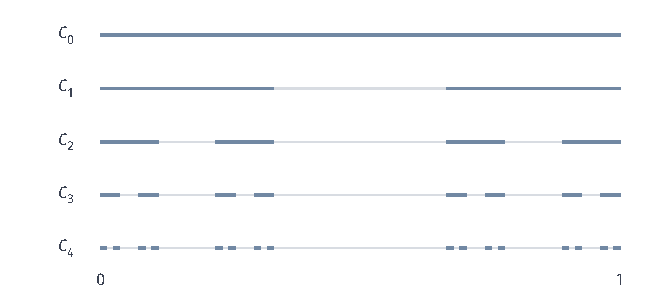
\includegraphics[width=112mm]{figures/01-mathematical-preliminaries-upper/01-mathematical-language-combinatorics-analysis-optimization/tikz/chapter3-concept-processes/cantor-deletion.pdf}
 \caption{蓝线表示$C_0,\ldots,C_4$，每一步从上一行各闭区间中删去中间开三分之一。$C_n$由$2^n$个长度$3^{-n}$的闭区间组成，总长度为$(2/3)^n$；交集$C$的测度因此为零，但始终包含$0,1$。任何有限一行仍有正测度，不能把有限阶段当成最终零测集。}
 \label{fig:analysis-process-cantor-deletion}
\end{figure}

\paragraph{康托尔函数}
\label{sec:analysis-cantor-function}
康托尔集的长度为零，却仍可以承载函数的全部增长。下面用同一删除过程构造一个连续的非减函数：它在每个删去的区间上保持常数，因而在零测集$C$之外导数为零，却从$0$增加到$1$。

$C$中的点在每一步落在左或右保留区间，分别确定三进制表示的下一位为$0$或$2$，所以$C$中每点都有只含这两个数字的表示；示例~\ref{ex:set-measure-cantor-uncountable-null}已说明不同数字序列给出不同的点，因此这种表示唯一。
把三进制数字$0,2$分别改为二进制数字$0,1$，定义
\[
 x=\sum_{j=1}^\infty\frac{\varepsilon_j}{3^j},\qquad
 F(x)=\sum_{j=1}^\infty\frac{\varepsilon_j/2}{2^j},
 \qquad\varepsilon_j\in\{0,2\}.
\]
第二个级数由几何级数$\sum_j2^{-j}$控制，取值在$[0,1]$中；其中$x=1$取全为$2$的表示，$F(1)=1$。

$F$在$C$上不减。若$C$中两点$x<y$的三进制位首次在第$k$位不同，由示例~\ref{ex:set-measure-cantor-uncountable-null}中对首个不同位的估计，较大的$y$在该位取$2$，$x$取$0$。
于是$F(y)$在二进制第$k$位比$F(x)$多$2^{-k}$，而后续各位造成的反向差至多为$\sum_{j>k}2^{-j}=2^{-k}$，所以$F(x)\leq F(y)$。

再把$F$延拓到删去的区间上。若一个开区间在第$k$步删去，它的两端都在$C$中，三进制表示的前$k-1$位相同；左端点第$k$位为$0$而后全为$2$，右端点第$k$位为$2$而后全为$0$。
对应的二进制数分别是该位为$0$而后全为$1$、该位为$1$而后全为$0$，同一个尾和恒等式$\sum_{j>k}2^{-j}=2^{-k}$保证两值相等。
例如$1/3=0.0222\ldots_3$与$2/3=0.2000\ldots_3$都对应$1/2$。
在该开区间上把$F$定义为这个共同值，就得到整个$[0,1]$上的\term{康托尔函数}（Cantor function）。

下面验证康托尔函数的单调性、连续性与导数，并说明它的增长集中在$C$上。
\begin{example}[康托尔函数的连续性与导数]
单调与端点：$F$在$C$上不减，在每个删去区间上取两端的共同值，所以在$[0,1]$上不减，且$F(0)=0$、$F(1)=1$。

一致连续：在第$n$步的每个保留区间上，$C$中的点有相同的前$n$位三进制数字，$F$的值因而有相同的前$n$位二进制数字，都落在一个长$2^{-n}$的区间内；删去区间上的取值也在这个范围中。
所以$F$在每个第$n$步保留区间上的变化不超过$2^{-n}$。
相邻两个第$n$步保留区间之间至少隔着长$3^{-n}$的删去区间，因此两个相距小于$3^{-n}$的点之间至多涉及两个第$n$步保留区间，函数值之差不超过$2^{1-n}$。
对任意给定的误差上界，先选$n$使$2^{1-n}$小于它，再取$\delta=3^{-n}$，就得到一致连续性。

导数：$[0,1]\setminus C$是全部删去开区间的并，$F$在每个删去开区间内恒定，所以$F'=0$于$[0,1]\setminus C$。由于$m(C)=0$，$F'=0$在$[0,1]$上几乎处处成立。

不绝对连续：第$n$步的$2^n$个保留区间总长度为$(2/3)^n\to0$，但每个保留区间两端的$F$值恰好相差$2^{-n}$，端点变化的总和仍为$2^n\cdot2^{-n}=1$。
把定义~\ref{def:measurable-absolutely-continuous-function}中的误差界取为$1$：无论$\delta>0$多小，只要$(2/3)^n<\delta$，这组保留区间的总长度就小于$\delta$，端点变化之和却等于$1$，所以定义的要求不成立。
\end{example}

所以康托尔函数一致连续（因而连续）、几乎处处导数为零，全部增长$F(1)-F(0)=1$却集中在零测集$C$上。
第~\ref{sec:analysis-fundamental-calculus}节将用它说明，只知道函数连续且几乎处处可导，不能由导数的积分恢复端点变化。

\FloatBarrier

\section{一元函数的可测性和积分}
\label{sec:analysis-measurability-integration}
\label{sec:analysis-integration-average}
\label{sec:analysis-classical-integration}

第~\ref{sec:comb-set-measurement}节回答了怎样测量集合的大小。现在进一步问：函数在不同位置取不同的值时，怎样把这些值与所在范围的大小结合起来，得到一个累计量？
例如，长为$\ell$的一段区间上密度恒为$c$，总质量就是$c\ell$；密度随位置变化时，需要把这种计算推广到一般函数。
本节的自变量始终是一维实变量，有限区间$[a,b]$总设$a<b$；集合的大小始终用勒贝格测度$m$度量。

我们先沿输入区间分段取样，建立黎曼积分，并检验分割越来越细时取样结果能否稳定。
狄利克雷函数将说明，有些函数的非零取值虽然只落在零测集上，在任意短的区间上取样仍可能得到完全不同的累计。
为处理这种情形，我们利用该节的可测集合与勒贝格测度，改按函数取值划分输入：先规定哪些函数能够这样分层，再以简单函数的有限累计构造勒贝格积分。

这条路线上的几个条件各有分工：可测集合规定哪些范围允许测量，勒贝格测度给这些范围赋值，可测函数保证按取值划出的各层输入集合属于这些范围，可积条件再保证总累计有限。它们不能互相替代。

两种积分的定义及其关系明确之后，我们再研究累计函数与求导的联系、积分的运算法则、函数列与函数项级数的极限交换以及反常积分；每一步都说明所用的是哪种积分及相应的条件。

\subsection{黎曼定积分}
\label{sec:analysis-integral-definitions}
\label{sec:analysis-riemann-integral}

黎曼积分只用区间长度作权重：把输入区间切成有限个小段，研究小段越来越短时，取样累计能否趋于一个与取样无关的总量。这一构造只用到有限区间分割，还不需要一般可测集合上的积分。


\subsubsection{积分的定义}

构造从常数密度乘长度出发：先在每个小段上把函数当作常数，得到有限近似；再要求所有足够细的近似都接近同一个数。这种误差控制必须同时覆盖分割方式与取样点两种选择。


\paragraph{黎曼和}
要累计$f$在$[a,b]$上的取值，先把区间分成有限段。取
\[
 P:\quad a=x_0<x_1<\cdots<x_n=b,
\]
称$P$为一个分割，记$\Delta x_i=x_i-x_{i-1}$，$\lVert P\rVert=\max_i\Delta x_i$。细度$\lVert P\rVert$是最长小段的长度；令它趋零，要求每一段都变短，而不只是增加分割点的数量。
再在每个小区间中取样点$\xi_i\in[x_{i-1},x_i]$，用常数$f(\xi_i)$代表该段的函数值，得到
\[
 S(f,P,\xi)=\sum_{i=1}^n f(\xi_i)\Delta x_i.
\]
这称为\term{黎曼和}（Riemann sum）。若$f\geq0$，每项是一个矩形的面积；有负值时，位于横轴下方的矩形按负号计入，所以求和表示带符号的累计。
黎曼和同时依赖分割$P$与取样点$\xi$，积分的定义要求极限不受这两种选择影响。

\paragraph{黎曼积分}
区间分得越来越细时，不同取样方式所得的黎曼和仍可能不同。只有当这些取样结果都趋向同一个有限值时，才能把这个值作为函数在区间上的累计量。

\begin{definition}[黎曼积分]
\label{def:analysis-riemann-integral}
设$f:[a,b]\to\mathbb R$有界。若存在实数$A$，使对每个$\varepsilon>0$都存在$\delta>0$，当$\lVert P\rVert<\delta$时，不论怎样选取样点都有
\[
 |S(f,P,\xi)-A|<\varepsilon,
\]
则称$f$在$[a,b]$上\term{黎曼可积}（Riemann integrable），并称$A$为其\term{黎曼积分}（Riemann integral），记为$\int_a^bf(x)\,\mathrm dx$。
\end{definition}
定义中的$\delta$只依赖$\varepsilon$：只要分割足够细，无论分割点和取样点怎样选取，黎曼和都落在$A$附近。最简单的情形是常数函数$f(x)=c$，它的每个黎曼和都等于$c(b-a)$，所以积分为$c(b-a)$。对一般函数，直接检查全部取样并不方便，下一小节改用上和与下和判断共同极限是否存在。

\paragraph{定积分与积分变量}
固定被积函数和积分范围后，$\int_a^bf(x)\,\mathrm dx$是一个数，称为定积分；$a,b$分别为下限和上限，$x$为积分变量。积分变量只在积分式内部使用，换成$t$不改变结果：$\int_a^bf(x)\,\mathrm dx=\int_a^bf(t)\,\mathrm dt$。

端点还采用有向约定：$\int_b^af=-\int_a^bf$，$\int_a^af=0$。后面定义的勒贝格积分在固定范围上同样给出一个数，区间端点记号沿用这一约定，只是可积条件不同。

\subsubsection{可积性的要求}
\label{sec:analysis-integrability-requirements}

黎曼积分的定义只对有界函数提出，但有界性并不保证所有细分与取样得到共同极限。上和与下和把不同取样的可能结果夹在两个数之间，使可积性成为一个可以验证的误差条件。

\paragraph{上和与下和}
取样点可能选到小段中不同的函数值。为了同时控制全部选择，设$f$在$[a,b]$上有界，对分割$P$定义
\begin{equation}
 \begin{aligned}
 m_i&=\inf_{[x_{i-1},x_i]}f,\qquad M_i=\sup_{[x_{i-1},x_i]}f,\\
 L(f,P)&=\sum_i m_i\Delta x_i,\qquad
 U(f,P)=\sum_i M_i\Delta x_i.
 \end{aligned}
\label{eq:analysis-riemann-upper-lower-sums}
\end{equation}
$L(f,P)$称为下和，$U(f,P)$称为上和。由于$m_i\leq f(\xi_i)\leq M_i$，同一分割下的任意黎曼和都满足$L(f,P)\leq S(f,P,\xi)\leq U(f,P)$。这里用上确界和下确界而不用最大值和最小值，是因为有界函数在小段上未必取到最值。

\paragraph{Darboux判据}
加入新的分割点时，一个小段被拆成几段，每个子段上的下确界不小于原段的下确界，上确界不大于原段的上确界，所以下和不减、上和不增。任意两个分割都有公共加细，因而任意下和都不超过任意上和。于是可以定义下积分$\sup_PL(f,P)$与上积分$\inf_PU(f,P)$，并且下积分不超过上积分。

Darboux判据断言：有界函数$f$黎曼可积，当且仅当上积分与下积分相等；等价地，对每个$\varepsilon>0$存在分割$P$满足
\[
 U(f,P)-L(f,P)<\varepsilon.
\]
后两种说法的等价性直接来自定义。上下积分相等时，分别取下和、上和接近它们的两个分割，再取公共加细，即得上述小差；反之，若某个分割的上下和之差小于$\varepsilon$，上下积分之差也小于$\varepsilon$。

还须证明这一条件与黎曼积分的定义等价。先设上下和之差可以任意小。给定$\varepsilon>0$，固定一个满足$U(f,P_0)-L(f,P_0)<\varepsilon$的分割$P_0$，设它有$k$个内分割点，且$|f|\leq M$。对另一个分割$Q$，不含$P_0$分割点的小段都落在$P_0$的某一段内，可以沿用该段的上下界；跨过$P_0$分割点的小段至多$k$个，总长度至多为$k\lVert Q\rVert$，函数在其上的振幅至多为$2M$。因此
\[
 U(f,Q)-L(f,Q)\leq U(f,P_0)-L(f,P_0)+2Mk\lVert Q\rVert.
\]
令$\lVert Q\rVert$足够小，右侧便小于$2\varepsilon$。任意取样的黎曼和与上下积分的共同值都夹在$L(f,Q)$与$U(f,Q)$之间，所以二者之差小于$2\varepsilon$，这正是黎曼积分的定义。
反过来，若$f$按定义黎曼可积，取一个足够细的分割，在每个小段上分别选接近上确界和接近下确界的取样点。两组黎曼和都接近积分值，又分别接近$U(f,P)$与$L(f,P)$，所以上下和之差可以任意小。因此Darboux判据与黎曼积分的定义等价。

图~\ref{fig:analysis-process-riemann-upper-lower}显示分割加细怎样缩小上和与下和之间的差距。
\begin{figure*}[!htbp]
 \centering
 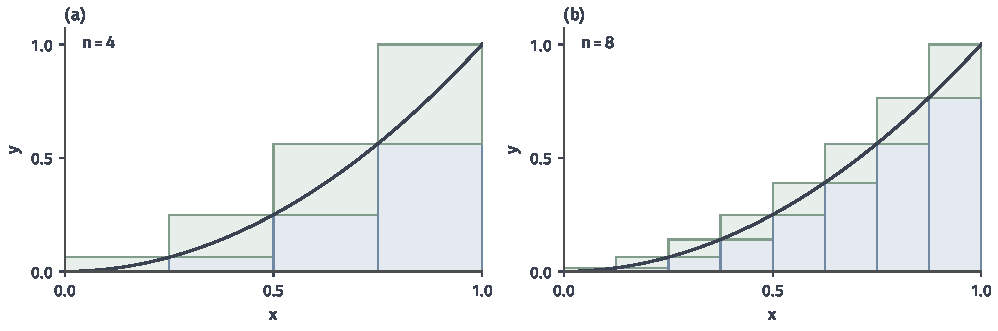
\includegraphics[width=169.0mm]{figures/01-mathematical-preliminaries-upper/01-mathematical-language-combinatorics-analysis-optimization/matplotlib/chapter3-concept-processes/riemann-upper-lower.pdf}
 \caption{对$[0,1]$上的$f(x)=x^2$，分别等分为4段、8段。蓝色矩形累计下和，补上绿色部分得到上和，黑线为函数图像。绿色部分的总面积就是$U_n-L_n=1/n$，从$1/4$降到$1/8$；Darboux判据要求这种差能任意小，而不只是在选定的某一张图中较小。}
 \label{fig:analysis-process-riemann-upper-lower}
\end{figure*}

\paragraph{连续函数的可积性}
Darboux判据首先用于连续函数。
若$f$在$[a,b]$上连续，则由闭区间上连续函数的性质，$f$有界且一致连续。给定$\varepsilon>0$，取$\delta>0$使输入距离小于$\delta$时，输出距离小于$\varepsilon/[2(b-a)]$。对细度小于$\delta$的分割，每段上的振幅$M_i-m_i$都不超过$\varepsilon/[2(b-a)]$，所以
\[
 U(f,P)-L(f,P)=\sum_i(M_i-m_i)\Delta x_i\leq\varepsilon/2<\varepsilon.
\]
因此闭区间上的连续函数黎曼可积。一致连续性在这里给出一个对所有小段同时适用的尺度$\delta$；若只在各点分别连续，所需的段长可能随位置变化。

\paragraph{有限间断点函数的可积性}
连续性是黎曼可积的充分条件，却不是必要条件。若有界函数只在有限个点不连续，可以先用很短的区间把这些点隔离，再在其余范围上使用连续性。

设$|f|\leq M$，其中$M>0$，不连续点为$c_1,\ldots,c_k$。给定$\varepsilon>0$，用总长度小于$\varepsilon/(4M)$的有限个开区间包住这些点；函数在这些小段上的振幅至多为$2M$，所以这些小段对$U-L$的贡献不超过$\varepsilon/2$。其余部分由有限个闭区间组成，$f$在其上连续，按连续函数情形的方法加细，可使它们的贡献也小于$\varepsilon/2$。把两部分的分割点合在一起，就得到$U(f,P)-L(f,P)<\varepsilon$，所以$f$黎曼可积。
例如只有有限个跳跃的分段连续有界函数，以及把连续函数在有限个点改为其他有限值所得的函数，都属于这种情形。

\subsubsection{黎曼积分的基本性质}

Darboux判据回答了哪些函数黎曼可积。后面合并相邻区间上的累计、建立微积分基本定理时，还要用到积分关于积分区间和被积函数的基本运算；这些性质都可以直接从黎曼和与上下和得到。

\paragraph{区间可加性}
若$f$在$[a,b]$上黎曼可积，则它在每个子区间上也黎曼可积：把子区间的端点加入分割后，上下和之差中属于该子区间的部分是一些非负项之和，不超过全区间上的差，再由Darboux判据即得。
对$a\leq c\leq b$，在$[a,c]$与$[c,b]$上分别取分割与取样点，合起来就是$[a,b]$上以$c$为分割点的分割，两侧黎曼和相加恰为全区间的黎曼和。令细度趋零，得到
\[
 \int_a^bf=\int_a^cf+\int_c^bf.
\]
结合有向端点约定，这个等式对$a,b,c$的任意顺序都成立，只要涉及的区间都在可积范围内。

\paragraph{加减}
若$f,g$在$[a,b]$上黎曼可积，对同一分割与同一组取样点，有$S(f\pm g,P,\xi)=S(f,P,\xi)\pm S(g,P,\xi)$。分割足够细时右侧两项分别接近$\int_a^bf$与$\int_a^bg$，所以$f\pm g$黎曼可积，且
\[
 \int_a^b\bigl(f(x)\pm g(x)\bigr)\,\mathrm dx=\int_a^bf(x)\,\mathrm dx\pm\int_a^bg(x)\,\mathrm dx.
\]

\paragraph{数乘}
若$f$在$[a,b]$上黎曼可积，$c$为实常数，则$S(cf,P,\xi)=cS(f,P,\xi)$，与$c\int_a^bf$的误差也只乘以$|c|$，所以$cf$黎曼可积，且
\[
 \int_a^bcf(x)\,\mathrm dx=c\int_a^bf(x)\,\mathrm dx.
\]

\paragraph{上下界估计}
若常数$\alpha,\beta$满足$\alpha\leq f\leq\beta$，每个黎曼和都夹在$\alpha(b-a)$与$\beta(b-a)$之间，所以
\[
 \alpha(b-a)\leq\int_a^bf(x)\,\mathrm dx\leq\beta(b-a).
\]
特别地，$|f|\leq M$时有$|\int_a^bf|\leq M(b-a)$；端点顺序颠倒时，右侧改用区间长度$|b-a|$。

以上结论只用到有限和及其极限，不依赖微积分基本定理。后面的运算法则统一采用勒贝格积分，其线性将从简单函数的构造另行建立。

\subsubsection{黎曼积分的局限}

第~\ref{sec:analysis-integrability-requirements}节已经证明，连续函数以及只有有限个间断点的有界函数都黎曼可积，但并非任意有界函数都能这样累计。下面用有理点集构造一个反例，再用同一个集合说明黎曼可积性在函数列的逐点极限下不能保持。


\paragraph{狄利克雷函数}
黎曼可积要求各段振幅乘长度的总和能够任意小。下面的有界函数在每个小段上的振幅都等于一，缩短区间无法减小这一误差。
\begin{example}[狄利克雷函数不黎曼可积]
\label{ex:analysis-dirichlet-not-riemann}
令$Q_0=\mathbb Q\cap[0,1]$，在$[0,1]$上定义$d(x)=\mathbb I_{Q_0}(x)$，称为狄利克雷函数。
每个非退化小区间都同时含有有理数和无理数，所以对任意分割$P$，每段都有$m_i=0$、$M_i=1$，从而
\[
 L(d,P)=0,\qquad U(d,P)=1.
\]
上下和之差恒为$1$，不随分割加细而减小，Darboux判据不成立。直接看黎曼和也是如此：不论分割多细，全部选有理取样点得到黎曼和$1$，全部选无理取样点得到$0$。因此$d$在$[0,1]$上不黎曼可积。
\end{example}
这里的困难不能靠加细分割解决：误差来自每个小区间内同时存在两种取值，而不是区间不够短。

第~\ref{sec:comb-set-measurement}节已经证明$m(Q_0)=0$、$m([0,1]\setminus Q_0)=1$。若不按相邻输入分组，而把取相同函数值的输入归为一组，取值$1$对应零测集$Q_0$，取值$0$对应其余部分，所需的有限计算便是
\[
 1\cdot m(Q_0)+0\cdot m([0,1]\setminus Q_0)=0.
\]
这提示我们改变分组依据：不再只用相邻输入组成的小区间代表函数，而允许把具有同一取值的输入归为一组，即使这组输入散布在许多位置。

黎曼积分在函数列的极限下也会遇到同样的障碍。
\begin{example}[有限点指示函数递增到狄利克雷函数]
\label{ex:analysis-finite-indicators-dirichlet}
将$Q_0$列举为$\{q_1,q_2,\ldots\}$，令$d_n=\mathbb I_{\{q_1,\ldots,q_n\}}$。
每个$d_n$有界，且只在$n$个点不连续，由有限间断点的结论黎曼可积；它在每个小段上的下确界为零，下和恒为零，所以$\int_0^1d_n(x)\,\mathrm dx=0$。
另一方面，对每个$x\in[0,1]$，$d_n(x)$关于$n$单调不减：若$x=q_k$，则$n\geq k$时$d_n(x)=1$；若$x$是无理数，则$d_n(x)$恒为零。所以$d_n$逐点递增到$d$，而由示例~\ref{ex:analysis-dirichlet-not-riemann}，$d$不黎曼可积。
\end{example}
可见各项都黎曼可积，并不保证逐点极限仍黎曼可积。后面将看到，按取值分层的新累计既能处理$d$，也能在非负单调逼近下保留积分的极限。

这并不否定黎曼积分在连续函数等情形中的作用。新的构造还必须证明，在原来黎曼可积的范围内，它与已有的积分相等。

\subsection{勒贝格定积分}
\label{sec:analysis-lebesgue-definite-integral}

狄利克雷函数只取两个值，两个取值集合都可测，因此可以按“函数值乘相应集合的测度”计算。
一般函数可能取无穷多个值，需要先把取值范围分成有限档，再逐步缩小档宽、提高截断高度。
每一档对应的输入集合可能散布在许多位置，不必是一个区间。

第~\ref{sec:comb-set-measurement}节的测量结构在这里各有分工：可测集族$\mathcal L(\mathbb R)$保证各档集合经可数次集合运算后仍可测量，勒贝格测度$m$给每一档赋予大小。
还缺的是函数一侧的条件：函数划出的各档输入集合是否可测。因此先引入可测函数，再依次定义简单函数的积分和非负函数的积分，最后检查有符号累计何时有限。
以下$E$总表示$\mathcal L(\mathbb R)$中的集合，用作函数的定义域或积分范围。

\subsubsection{可测函数}
\label{sec:analysis-measurable-functions}

按取值分层之前，先要求函数满足一个资格条件：每一层的输入集合都属于可测集族。这个条件只保证各层能够测量，不保证总累计有限。


\paragraph{可测函数的定义}
可测集是输入范围中的集合；可测函数则要保证，指定输出的一段取值范围后，落入这段范围的输入仍组成可测集。
例如要计算取值大于$c$的输入占多大长度，必须先有$\{x\in E:f(x)>c\}\in\mathcal L(\mathbb R)$，才能用$m$给它赋值。

一般地，输出范围可取任意Borel集$B\subseteq\mathbb R$，分层累计依次涉及三个对象：
\[
 B\longmapsto f^{-1}(B)=\{x\in E:f(x)\in B\}
 \longmapsto m(f^{-1}(B)).
\]
测度$m$作用在输入集合$f^{-1}(B)$上，而不是作用在函数值上。可测函数要求链中的原像$f^{-1}(B)$总属于$\mathcal L(\mathbb R)$，这样第二步才有意义。
\begin{definition}[可测函数]
\label{def:analysis-measurable-function}
设$E\in\mathcal L(\mathbb R)$。函数$f:E\to\mathbb R$称为（勒贝格）\term{可测函数}（measurable function），若对每个Borel集$B\subseteq\mathbb R$，原像$f^{-1}(B)$都属于$\mathcal L(\mathbb R)$。等价地，只需对每个$a\in\mathbb R$有$\{x\in E:f(x)>a\}\in\mathcal L(\mathbb R)$。扩展实轴$[-\infty,+\infty]$的Borel结构由射线$(a,+\infty]$（$a\in\mathbb R$）生成，扩展实值函数按此结构作同样定义。
\end{definition}
阈值条件已经足够，原因有两点。第一，原像运算保持补集与可数并，所以使原像可测的输出集合$B$全体构成一个$\sigma$代数。第二，射线$(a,\infty)$生成实轴的Borel $\sigma$代数，所以这个$\sigma$代数一旦包含全部射线，就包含全部Borel集。
因此，验证可测性时通常只需检查阈值集合$\{f>a\}$，使用时则可以直接调用Borel原像条件。

例如一档取值$[u,v)$对应$\{u\leq f<v\}$，它是Borel集$[u,v)$的原像，因而可测。
对于狄利克雷函数，任一Borel集的原像只可能是$\varnothing,Q_0,[0,1]\setminus Q_0,[0,1]$之一，它们都勒贝格可测。
所以$d$虽不黎曼可积，却已经具备新构造所需的分层资格；当然，可测性本身还不能替任意函数保证积分有限。

反过来，若$A\subseteq E$不是可测集，指示函数$\mathbb I_A$就不可测，因为$\{\mathbb I_A>1/2\}=A$。
此时取值$1$所在的输入集合无法测量，“取值乘测度”的规则也就无从使用。

\paragraph{可测函数与连续函数的关系}
新的函数范围应包含原来熟悉的连续函数，同时容纳促使我们改变积分构造的狄利克雷函数。
若$E$是区间，连续函数$f:E\to\mathbb R$可测：开集的原像是$E$中的相对开集，即某个开集与$E$的交，因而是Borel集，也就勒贝格可测。反之，可测函数不必连续：狄利克雷函数的两个取值集合都勒贝格可测，所以它可测，却在每一点间断。

两者还能通过零测集上的改值联系起来。若$f$可测、$g=f$几乎处处，则对每个$a$，阈值集合$\{g>a\}$与$\{f>a\}$只相差某个零测集的子集；勒贝格测度完备，零测集的子集仍可测，所以$g$也可测。
因此只在零测集上改变取值，既不影响可测性，也不改变后面定义的积分；但这种改值可能破坏连续性，例如把零函数在$Q_0$上改为一，就得到处处不连续的狄利克雷函数。

\paragraph{可测函数的运算}
分层累计还要用于函数的加减、相乘和复合，因此应先保证这些运算不会把函数带出可测范围。
实值可测函数的和、积、绝对值、最大值与最小值仍可测。以和为例，
\[
 \{f+g>a\}=\bigcup_{q\in\mathbb Q}\bigl(\{f>q\}\cap\{g>a-q\}\bigr),
\]
右侧为可数个可测集合的并。

连续实函数$\phi$与可测函数复合所得的$\phi\circ f$仍可测。由于开集生成Borel $\sigma$代数，只需检查开集$B$的原像：$(\phi\circ f)^{-1}(B)=f^{-1}(\phi^{-1}(B))$，而$\phi^{-1}(B)$仍是开集。因而平方和绝对值可测，再由$fg=((f+g)^2-(f-g)^2)/4$得到乘积可测；最大值与最小值可由$\max\{f,g\}=(f+g+|f-g|)/2$与$\min\{f,g\}=(f+g-|f-g|)/2$得到。商在分母不为零的可测集合上可测；若要扩展到全域，需另行指定零点处的可测取值。

复合时，连续函数必须放在外层。若外层只是勒贝格可测函数，它的原像只保证是勒贝格可测集，未必是Borel集，再取内层函数的原像就可能不可测；本章不需要这种复合。扩展实值运算还要排除$\infty-\infty$等未定义形式。

\paragraph{可测函数列的极限}
后面要对函数列的极限求积分，因此还要确认极限运算不会离开可测函数的范围。
可数个可测函数的上确界、下确界可测，例如$\{\sup_nf_n>a\}=\bigcup_n\{f_n>a\}$。因此
\[
 \liminf_nf_n=\sup_N\inf_{n\geq N}f_n,\qquad
 \limsup_nf_n=\inf_N\sup_{n\geq N}f_n
\]
都可测；逐点极限存在时，它等于上、下极限，也可测。若极限只在零测集外存在，可在例外集上取值零，由零测改值的结论仍得到可测函数。
相比之下，连续函数的逐点极限可能不连续，例如$[0,1]$上$x^n$的逐点极限在$x=1$处跳跃。可测函数类对逐点极限封闭，所以用函数列逼近时不会离开这一类对象。

\subsubsection{积分的定义}

勒贝格测度给出了可测集合的大小。积分的定义分三步：先用测度计算只取有限个值的简单函数，再用简单函数从下方逼近一般非负可测函数，最后通过正负分解处理有符号函数。


\paragraph{简单函数的积分}
按取值分层累计时，最简单的情形是函数只取有限个值。只取有限个实数值的可测函数称为\term{简单函数}（simple function）。若$s$取值$a_1,\ldots,a_m$，则$E_j=\{x:s(x)=a_j\}$两两不交且可测，函数可写为$s=\sum_ja_j\mathbb I_{E_j}$。
简单函数正是“有限档”的分层：每一档是一个可测集，函数在其上取常值，该档的贡献就应为$a_jm(E_j)$。
各档两两不交，每个输入只计一次，这正是勒贝格测度的有限可加性所支持的累计方式。
下面先对非负取值定义积分，有负取值的情形稍后拆成正负两部分处理。
\begin{definition}[非负简单函数的积分]
\label{def:analysis-simple-function-integral}
设$s=\sum_{j=1}^m a_j\mathbb I_{E_j}$是$E$上的简单函数，其中$a_j\geq0$、$E_j\subseteq E$可测且两两不交，则定义
\begin{equation}
 \int_Es\,\mathrm dm=\sum_{j=1}^m a_jm(E_j).
\label{eq:analysis-simple-integral}
\end{equation}
这里约定$0\cdot\infty=0$，允许积分为$+\infty$。
\end{definition}
同一简单函数可能有不同的表示，需要确认计算结果不依赖分组方式。
把两种表示中的集合两两求交，作为公共细分，每个新块可测且函数在其上取固定值；用测度的有限可加性拆开原来的各项，两种表示便化为同一个有限和。
同一方法还证明，非负简单函数的加法、非负数乘和大小关系都与积分相容。

这个定义把集合的测度与函数的累计连接起来。对可测$A\subseteq E$，$\int_E\mathbb I_A\,\mathrm dm=m(A)$，即测量一个集合等于对它的指示函数积分；对常数$c\geq0$，则有$\int_Ec\,\mathrm dm=cm(E)$。
特别地，示例~\ref{ex:analysis-dirichlet-not-riemann}中的狄利克雷函数是简单函数，前面提示的分层计算现在就是它的积分：$\int_{[0,1]}d\,\mathrm dm=1\cdot m(Q_0)+0\cdot m([0,1]\setminus Q_0)=0$。
这个值由可测集$Q_0$及其补集的测度直接给出，计算没有把每个点的零长度逐一相加；那样的做法对不可数集合$[0,1]\setminus Q_0$并无意义。

图~\ref{fig:integral-value-layers}用同一函数比较两种分组方式。黎曼和的每个组是相邻输入组成的区间；简单函数的一档则由取值条件确定，输入集合可以分成互相分离的几段。

\begin{figure*}[htbp]
 \centering
 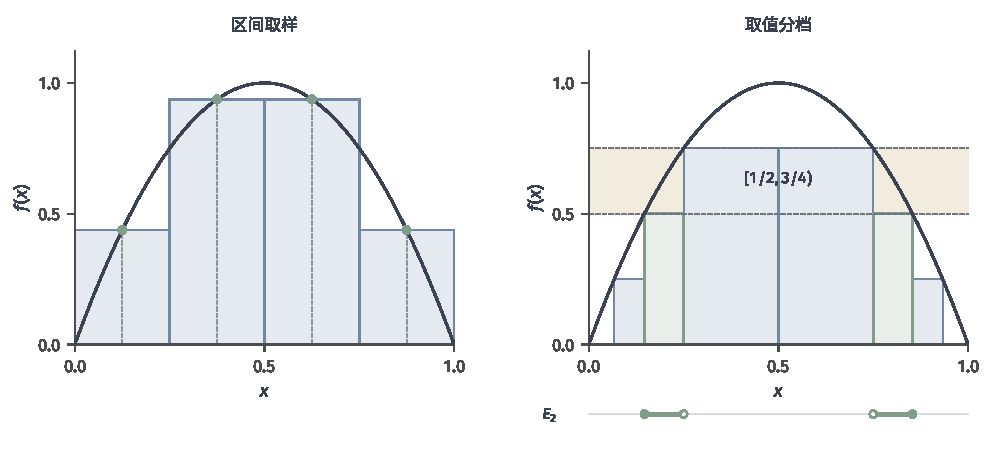
\includegraphics[width=169mm]{figures/01-mathematical-preliminaries-upper/01-mathematical-language-combinatorics-analysis-optimization/matplotlib/integral-value-layers/figure.pdf}
 \caption{对同一函数$f(x)=4x(1-x)$（$0\leq x\leq1$）作有限近似。左侧等分输入区间为四段，在中点取样形成黎曼和，矩形可高于或低于曲线。右侧将输出范围按$1/4$分档，在$E_j=\{x:j/4\leq f(x)<(j+1)/4\}$上取下界$a_j=j/4$；绿色标出$E_2=\{1/2\leq f<3/4\}$对应的两个输入区间，它们的总测度乘$1/2$给出这一档的贡献。下方单独画出$E_2$并标明端点。最大值处的单点不影响积分，图中略去。左侧累计为$\sum_i f(\xi_i)\Delta x_i$，右侧简单函数的累计为$\sum_j a_jm(E_j)$。勒贝格构造加细的是取值档，权重仍来自输入集合的测度。}
 \label{fig:integral-value-layers}
\end{figure*}


\paragraph{非负勒贝格积分}
一般非负可测函数可能取无穷多个值，不能直接套用有限和。但它可以由简单函数从下方逐步逼近，这为用简单函数定义一般积分提供了依据。
若只把取值舍入到网格，无界函数仍会取无穷多个网格值；若只截断高度，截断后的函数仍可能取连续多个值。因此同时做两件事：把高度截断到$n$，并把取值向下舍入到步长$2^{-n}$的网格，得到
\begin{equation}
 \begin{aligned}
 s_n(x)&=\sum_{k=0}^{n2^n-1}\frac{k}{2^n}
  \mathbb I_{\{k/2^n\leq f<(k+1)/2^n\}}(x)\\
 &\quad+n\mathbb I_{\{f\geq n\}}(x).
 \end{aligned}
\label{eq:analysis-canonical-simple-approximation}
\end{equation}
每个$s_n$只取有限个值，取值集合可测，且$0\leq s_n\leq f$。从$n$到$n+1$时网格加细、截断高度增大，所以下方近似不减。若$f(x)$有限，则$n>f(x)$以后舍入误差小于$2^{-n}$；若$f(x)=\infty$，则$s_n(x)=n$。因此$s_n\uparrow f$逐点成立，称$(s_n)$为$f$的规范简单逼近。
反过来，由第~\ref{sec:analysis-measurable-functions}节，可测函数列的逐点极限仍可测，所以非负函数可测，当且仅当它是一列非负简单函数的逐点递增极限。
这些$s_n$的积分是否趋于$f$的积分，要等定义了一般积分后，由单调收敛定理回答。

每个满足$0\leq s\leq f$的简单函数$s$都给出$f$累计的一个下界$\int_Es\,\mathrm dm$，规范简单逼近又说明这些下方函数可以逐点任意接近$f$。因此取全部这样的下界的上确界，作为$f$的累计。
\begin{definition}[非负勒贝格积分]
\label{def:analysis-nonnegative-lebesgue-integral}
若$f:E\to[0,\infty]$可测，定义
\begin{equation}
 \int_Ef\,\mathrm dm
 =\sup\left\{\int_Es\,\mathrm dm:
       s\text{为非负简单函数},\ 0\leq s\leq f\right\}.
\label{eq:analysis-nonnegative-lebesgue-integral}
\end{equation}
这称为$f$在$E$上的非负\term{勒贝格积分}（Lebesgue integral），值可为$+\infty$。
\end{definition}
上确界取遍所有下方简单函数，保留了它们能累计到的全部贡献，结果不依赖某一列特定的逼近，也不依赖取样。

对可测$A\subseteq E$，记$\int_Af\,\mathrm dm=\int_Ef\mathbb I_A\,\mathrm dm$。常写$\int_Ef(x)\,\mathrm dx$代替$\int_Ef\,\mathrm dm$；$E=[a,b]$时也写$\int_a^bf(x)\,\mathrm dx$，并沿用有向端点约定。

对具体函数，可以用区间上的阶梯函数从上下两侧夹住这个上确界。
\begin{example}[用阶梯函数计算恒等函数的积分]
\label{ex:analysis-step-functions-identity}
取$f(x)=x$，把$[0,1]$等分为$n$段，前$n-1$段取左闭右开区间，最后一段取闭区间。在第$i$段上取下界$(i-1)/n$，得到简单函数$\ell_n\leq f$；取上界$i/n$，得到简单函数$u_n\geq f$。它们的积分为
\[
 \int_{[0,1]}\ell_n\,\mathrm dm=\sum_{i=1}^n\frac{i-1}{n}\cdot\frac1n=\frac{n-1}{2n},\qquad
 \int_{[0,1]}u_n\,\mathrm dm=\sum_{i=1}^n\frac in\cdot\frac1n=\frac{n+1}{2n}.
\]
例如两段时下方积分为$1/4$，四段时为$3/8$。
由定义，$\int_{[0,1]}f\,\mathrm dm\geq\int_{[0,1]}\ell_n\,\mathrm dm$。另一方面，任一简单函数$0\leq s\leq f$也满足$s\leq u_n$，简单函数积分的单调性给出$\int s\leq\int u_n$；对$s$取上确界，得$\int_{[0,1]}f\,\mathrm dm\leq\int_{[0,1]}u_n\,\mathrm dm$。
令$n\to\infty$，两侧界都趋于$1/2$，所以$\int_{[0,1]}x\,\mathrm dm=1/2$。
\end{example}
下方阶梯只用到上确界定义中的一部分简单函数；上方阶梯则通过单调性限制了全部下方简单函数，两者合起来确定积分值。
图~\ref{fig:analysis-simple-integral}用$f(x)=x^2$展示同样的下方逼近。
\begin{figure*}[htbp]
 \centering
 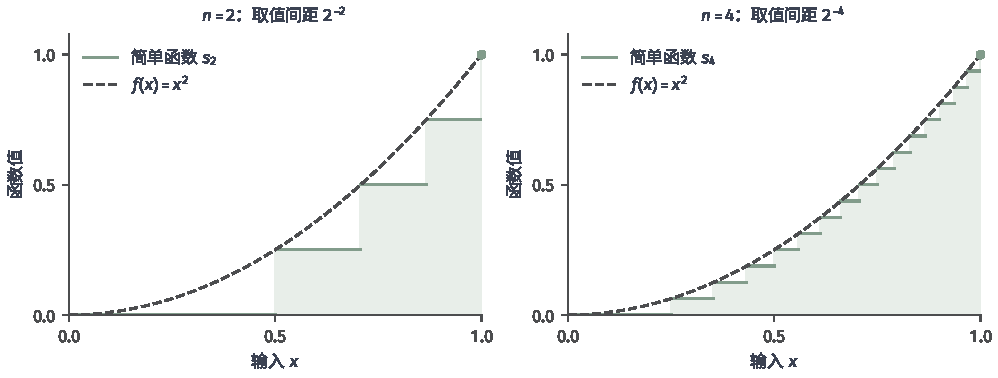
\includegraphics[width=169.0mm]{figures/01-mathematical-preliminaries-upper/01-mathematical-language-combinatorics-analysis-optimization/matplotlib/analysis-simple-integral/figure.pdf}
 \caption{$f(x)=x^2$在$[0,1]$上的简单函数逼近。图中将区间分别等分为两段、四段，在每段取函数下界，按高度乘长度求和；加细后下方累计增大，逼近积分$1/3$。简单函数还允许用一般可测集合代替图中的区间。}
 \label{fig:analysis-simple-integral}
\end{figure*}

\paragraph{有符号勒贝格积分}
非负函数的各部分贡献只会累加；有正负值时，还必须防止两个无穷总量相减。
对实值可测$f$，令$f^+=\max\{f,0\}$、$f^-=\max\{-f,0\}$，则$f=f^+-f^-$、$|f|=f^++f^-$，正负两部分均非负可测。
只要它们的积分不同时为无穷，就定义
\[
 \int_Ef\,\mathrm dm=\int_Ef^+\,\mathrm dm-\int_Ef^-\,\mathrm dm.
\]
两部分中恰有一个为无穷时，积分为$+\infty$或$-\infty$；两部分都为无穷时，差没有定义，也不能通过选择某种抵消次序给它指定一个有限的勒贝格积分。

\subsubsection{可积性的要求}

可测性保证各取值层可以测量，非负积分的定义给出一个确定的扩展实数值，但两者都不保证累计有限。
要使有符号积分成为有限实数，正负两部分的积分都必须有限；下面用绝对值的积分统一表述这一要求。

\begin{definition}[勒贝格可积函数]
\label{def:analysis-integrable-function}
若实值可测$f:E\to\mathbb R$满足
\begin{equation}
 \int_E|f|\,\mathrm dm<\infty,
\label{eq:analysis-absolute-integrability}
\end{equation}
则称$f$在$E$上勒贝格可积，也称\term{绝对可积}（absolutely integrable）。其有符号勒贝格积分是有限实数。
\end{definition}
由于$0\leq f^\pm\leq|f|$，凡在$f^\pm$下方的简单函数也在$|f|$下方，所以$\int_Ef^\pm\,\mathrm dm\leq\int_E|f|\,\mathrm dm<\infty$，这一定义确实给出有限的有符号积分。本节未附“黎曼”或“反常”限定的可积性均指这一绝对可积条件。

\paragraph{可积与正负部分}
可积性同时检查正、负两部分，而不只看抵消后的结果。
非负可测函数总有非负勒贝格积分，但这个值未必有限：常数一在$\mathbb R$上的积分为$+\infty$，所以它有积分值却不可积。
对有符号函数，有限积分要求正负部分的积分都有限，这与式~\eqref{eq:analysis-absolute-integrability}等价；等价性将在下一小节由非负积分的加法证明。

正负两部分都为无穷时，即使对称区间上的累计恒为零，也得不到勒贝格积分。
\begin{example}[符号函数在实轴上没有勒贝格积分]
\label{ex:analysis-sign-function-no-integral}
在$\mathbb R$上令$f=\mathbb I_{(0,\infty)}-\mathbb I_{(-\infty,0)}$，即原点处取零的符号函数。它的正部和负部分别为$f^+=\mathbb I_{(0,\infty)}$与$f^-=\mathbb I_{(-\infty,0)}$，所以
\[
 \int_{\mathbb R}f^+\,\mathrm dm=m((0,\infty))=+\infty,\qquad
 \int_{\mathbb R}f^-\,\mathrm dm=m((-\infty,0))=+\infty.
\]
两部分都为无穷，按定义$f$没有有符号勒贝格积分，当然也不可积。
另一方面，对每个$R>0$，$\int_{[-R,R]}f\,\mathrm dm=m((0,R])-m([-R,0))=R-R=0$，对称截断上的累计恒为零。
\end{example}
对称截断的零值来自正负无穷总量的成对相消，并不说明两部分有限。所以有限的有符号勒贝格积分必然来自绝对可积函数，不存在由正负无穷抵消得到的有限值。

\paragraph{有界性与可积性}
判断可积时，函数的大小与积分范围的测度必须一起考虑。
若$m(E)<\infty$且$|f|\leq M$，每个满足$0\leq s\leq|f|$的简单函数都不超过$M\mathbb I_E$，所以$\int_E|f|\,\mathrm dm\leq Mm(E)<\infty$。因此有限测度集合上的有界可测函数可积；狄利克雷函数就是这样在$[0,1]$上可积的。
在无穷测度范围上，有界性不足，实轴上的常数一已经说明这一点。
反过来，无界也未必不可积：第~\ref{sec:analysis-improper-integrals}节将算出$x^{-1/2}$在$(0,1)$上的积分等于$2$。
因此“有界”既不是可积的必要条件，也只在有限测度范围上构成充分条件。

\subsubsection{积分的性质}
\label{sec:analysis-lebesgue-basic-properties}

定义已经给出累计值，现在检查它是否保持加法、大小关系与积分范围的分拆。
先从简单函数和上确界证明非负情形，再用正负分解处理有限的有符号积分；以下的积分均关于勒贝格测度。

\paragraph{非负勒贝格积分的性质}
简单函数的积分具有线性与单调性，现在从上确界定义把这些性质推广到一般非负可测函数。证明只用前面建立的集合测度性质，所得结论为后面的累计函数和微积分基本定理提供依据。
\begin{theorem}[非负勒贝格积分的线性与单调性]
\label{lem:analysis-nonnegative-integral-properties}
设$E\in\mathcal L(\mathbb R)$，$f,g:E\to[0,\infty]$可测，$\alpha,\beta$为非负实数。
若$f\leq g$几乎处处，则$\int_Ef\,\mathrm dm\leq\int_Eg\,\mathrm dm$；
在$0\cdot\infty=0$的约定下，还有
\[
 \int_E(\alpha f+\beta g)\,\mathrm dm
 =\alpha\int_Ef\,\mathrm dm+\beta\int_Eg\,\mathrm dm.
\]
若$f=g$几乎处处，则它们的非负积分相同。
\end{theorem}
\begin{proof}
逐点单调性直接来自定义：每个简单函数$0\leq s\leq f$也满足$s\leq g$。
若$N$为零测集，简单函数在$N$上的积分为零。
对$f,g$在$E\setminus N$上相等的情形，将任意$0\leq s\leq f$在$N$上置零，
所得简单函数不超过$g$且积分未变。取上确界得$\int f\leq\int g$，反向相同；
几乎处处的单调性也可先作这项零测修改。

对加法，任取非负简单函数$s\leq f$、$t\leq g$，简单函数的有限线性给出
$\int(f+g)\geq\int s+\int t$。分别取上确界，得到
$\int(f+g)\geq\int f+\int g$。若右侧为无穷，这已给出等式；以下设右侧有限。
反向需要检查每个下方简单函数的累计。取任意非负简单函数
$u=\sum_{j=1}^m a_j\mathbb I_{E_j}\leq f+g$，其中$a_j>0$、$E_j$两两不交，
并取规范简单逼近$s_n\uparrow f$、$t_n\uparrow g$。
固定$c\in(0,1)$，令$E_{j,n}=E_j\cap\{s_n+t_n\geq ca_j\}$。
因$s_n+t_n\uparrow f+g$且$f+g\geq a_j$于$E_j$，有$E_{j,n}\uparrow E_j$。
第~\ref{sec:analysis-set-measure-continuity}节的测度递增连续性及简单函数的线性给出
\[
 \begin{aligned}
 c\int_Eu\,\mathrm dm
 &=\lim_n c\sum_j a_jm(E_{j,n})\\
 &\leq\liminf_n\left(\int_Es_n\,\mathrm dm+\int_Et_n\,\mathrm dm\right)\\
 &\leq\int_Ef\,\mathrm dm+\int_Eg\,\mathrm dm.
 \end{aligned}
\]
先令$c\uparrow1$，再对所有这样的$u$取上确界，便得到反向不等式。
正数倍的结论由$s\leq\alpha f$与$s/\alpha\leq f$在定义中的一一对应推出；
零数倍按约定处理，再与加法结合即得一般结论。
整个证明只使用简单函数的有限和、积分的上确界与集合测度的连续性，没有使用一般函数的单调收敛定理。
\end{proof}

\paragraph{有符号勒贝格积分的性质}
有正负值时，实线性要求所有参与相减的总量都有限，绝对可积性正好保证这一点。
下面同时证明可积性判别、有限线性、比较与绝对值估计。
\begin{theorem}[有符号勒贝格积分的基本性质]
\label{thm:analysis-signed-integral-properties}
设$E\in\mathcal L(\mathbb R)$，$f,g:E\to\mathbb R$可测。
函数$f$勒贝格可积，当且仅当$\int_E f^+\,\mathrm dm$与$\int_E f^-\,\mathrm dm$都有限。
若$f,g$勒贝格可积，$\alpha,\beta\in\mathbb R$，则$\alpha f+\beta g$也可积，且
\[
 \int_E(\alpha f+\beta g)\,\mathrm dm
 =\alpha\int_Ef\,\mathrm dm+\beta\int_Eg\,\mathrm dm.
\]
对上述可积的$f,g$，$f\leq g$几乎处处时有$\int_E f\,\mathrm dm\leq\int_E g\,\mathrm dm$，并且
\[
 \left|\int_Ef\,\mathrm dm\right|\leq\int_E|f|\,\mathrm dm.
\]
若$f$可积且$g=f$几乎处处，则$g$也可积，积分与$f$相同。
\end{theorem}
\begin{proof}
由$|f|=f^++f^-$及非负积分的加法，
$\int|f|=\int f^++\int f^-$，所以绝对积分有限等价于正负两项均有限。
再检查有符号积分与正负分解以外的表示是否相容。若$f=u-v$，其中$u,v$非负且可积，
则$f^+,f^-\leq u+v$，故$f$可积；非负恒等式$u+f^-=v+f^+$积分后可移去有限项，得到
$\int f=\int u-\int v$。

对可积$f,g$，$|f+g|\leq|f|+|g|$保证和可积。
将$f+g=(f^++g^+)-(f^-+g^-)$代入刚才的分解结论，再用非负加法，得到
$\int(f+g)=\int f+\int g$。正数倍沿用非负缩放，负数倍交换正负部分，零数倍直接成立，因而实线性成立。
若$f\leq g$几乎处处，可积差$g-f$的积分非负，移项即得比较关系。
定义中的正负分解与实数三角不等式给出
$|\int f|\leq\int f^++\int f^-=\int|f|$。
最后，若$f=g$几乎处处，则$g$可测；把非负积分的零测修改不变性分别用于$|f|,|g|$及正负部分，便得$g$可积且积分相同。
\end{proof}

证明中的每次移项都只移去有限值，没有通过正负无穷的抵消得到有限值。非负积分可以等于无穷，但有符号线性中的移项必须满足上述有限性条件。

\paragraph{零积分与零测例外}
非负函数没有正负抵消，积分为零应当意味着它的正值只落在零测范围内。
下面把这一判断写成等价条件，供后面比较两种积分时使用。
\begin{theorem}[非负函数的零积分判别]
\label{thm:analysis-zero-integral}
设$E\in\mathcal L(\mathbb R)$，$f:E\to[0,\infty]$可测，则
\[
 \int_Ef\,\mathrm dm=0\quad\Longleftrightarrow\quad f=0\ \text{几乎处处}.
\]
特别地，实值可测$f$满足$\int_E|f|\,\mathrm dm=0$当且仅当$f=0$几乎处处。
\end{theorem}
\begin{proof}
若积分为零，对每个正整数$k$，$f\geq k^{-1}\mathbb I_{\{f\geq1/k\}}$，故
$0\geq k^{-1}m(\{f\geq1/k\})$。这些集合都零测，而
$\{f>0\}=\bigcup_{k\geq1}\{f\geq1/k\}$，所以$f=0$几乎处处。
反之，非负积分的零测修改不变性表明$f$与零函数的积分相等。将结论用于$|f|$便得最后一条。
\end{proof}
对有正负值的$f$，仅有$\int f=0$不能推出$f=0$几乎处处，例如$f(x)=x$在$[-1,1]$上的积分为零。

\paragraph{积分范围的可加性}
函数值可以相加，积分范围也可以分拆；后者要保持的是可测集合的不交并。
下面从测度的可数可加性直接证明这一性质，不提前使用函数列的收敛定理。
\begin{theorem}[勒贝格积分的区域可加性]
\label{thm:analysis-integral-set-additivity}
设$A_n\in\mathcal L(\mathbb R)$两两不交，$A=\bigcup_{n\geq1}A_n$。
若$f:A\to[0,\infty]$可测，则
\[
 \int_Af\,\mathrm dm=\sum_{n=1}^{\infty}\int_{A_n}f\,\mathrm dm,
\]
允许等式两侧为无穷。若$f$实值且在$A$上绝对可积，同一等式成立，且右侧绝对收敛。
对可测$B,C$及在$B\cup C$上绝对可积的实值$f$，还有
\[
 \int_{B\cup C}f=\int_Bf+\int_Cf-\int_{B\cap C}f.
\]
特别地，$C\subseteq B$时有$\int_{B\setminus C}f=\int_Bf-\int_Cf$。
\end{theorem}
\begin{proof}
非负积分的有限区域加法来自指示函数恒等式与非负线性。
因此$\int_A f\geq\sum_{n=1}^N\int_{A_n}f$对每个$N$成立，取部分和的上确界得到一个方向。
反向取任意简单函数$0\leq s=\sum_{j=1}^r c_j\mathbb I_{E_j}\leq f$，其中$c_j>0$且$E_j$两两不交、均包含于$A$。
测度的可数可加性及有限和与非负级数的合并给出
\[
 \int_As\,\mathrm dm
 =\sum_{j=1}^r c_j\sum_{n\geq1}m(E_j\cap A_n)
 =\sum_{n\geq1}\int_{A_n}s\,\mathrm dm
 \leq\sum_{n\geq1}\int_{A_n}f\,\mathrm dm.
\]
对全部这样的$s$取上确界，得到反向不等式。

若$f$在$A$上绝对可积，先对$|f|$使用非负结论，得到
$\sum_n|\int_{A_n}f|\leq\sum_n\int_{A_n}|f|=\int_A|f|<\infty$。
再分别对$f^+,f^-$使用等式并相减，便得到有符号版本。
最后，将有限实线性用于
$\mathbb I_{B\cup C}+\mathbb I_{B\cap C}=\mathbb I_B+\mathbb I_C$即得容斥式，包含情形再化为差集式。
\end{proof}
非负函数的积分为无穷时，区域相加的等式仍成立，但不能把它随意改写为含$\infty-\infty$的差。

\subsubsection{与黎曼积分的关系}

新的定义既要处理原来无法累计的函数，也要与已有的数值相容。下面先证明新定义没有改变黎曼可积函数的积分值，再用不连续点的测度准确刻画哪些函数黎曼可积。


\paragraph{黎曼积分与勒贝格积分的关系}
改变累计方式之后，必须检验原来已经能够计算的积分是否得到保留。
下面把黎曼上下和看作简单函数的积分，借助可测的上下包络及其零测差证明两种积分一致。
\begin{theorem}[黎曼积分与勒贝格积分的一致性]
\label{thm:analysis-riemann-lebesgue-consistency}
设$a<b$，$f:[a,b]\to\mathbb R$有界且黎曼可积。
则$f$勒贝格可测、勒贝格可积，且
\[
 \int_a^bf(x)\,\mathrm dx\ \text{（黎曼）}
 =\int_{[a,b]}f\,\mathrm dm\ \text{（勒贝格）}.
\]
反向蕴含不成立：有界勒贝格可积函数未必黎曼可积。
\end{theorem}
\begin{proof}
设$|f|\leq M$。由Darboux判据，可取一列分割$P_n$，后一个是前一个的加细，并使$U(f,P_n)-L(f,P_n)<1/n$。
在$P_n$的每个小区间内部，令下阶梯函数$\ell_n$取该段的下确界$m_i$，上阶梯函数$u_n$取上确界$M_i$；
有限个分割点上的取值不影响积分，可以都取$f$的值。于是$\ell_n\leq f\leq u_n$，它们都是简单函数，
且$\int\ell_n\,\mathrm dm=L(f,P_n)$、$\int u_n\,\mathrm dm=U(f,P_n)$。加细使$\ell_n$逐点不减、$u_n$逐点不增。
令$\ell=\sup_n\ell_n$、$u=\inf_nu_n$。它们可测，因为$\{\ell>c\}=\bigcup_n\{\ell_n>c\}$是可数个可测集合的并，$u$同理；并且$\ell\leq f\leq u$。
非负可测函数$u-\ell$对每个$n$都满足$u-\ell\leq u_n-\ell_n$，由积分的单调性，
\[
 0\leq\int_{[a,b]}(u-\ell)\,\mathrm dm\leq U(f,P_n)-L(f,P_n)<\frac1n,
\]
所以这个积分为零。由定理~\ref{thm:analysis-zero-integral}，$\{u\neq\ell\}$是零测集。$f$只在这个零测集上可能与可测函数$\ell$不同，
而勒贝格测度完备，所以$f$勒贝格可测。有限区间上的有界可测函数绝对可积，故可使用有符号积分的比较关系。
最后，每个$n$都有$L(f,P_n)=\int\ell_n\leq\int f\leq\int u_n=U(f,P_n)$（有符号情形先给$f$加常数$M$使之非负，再用有限线性移去常数），
两端都趋于黎曼积分，所以勒贝格积分等于黎曼积分。

示例~\ref{ex:analysis-dirichlet-not-riemann}中的狄利克雷函数有界、勒贝格可积而不黎曼可积，所以反向蕴含不成立。
\end{proof}

\paragraph{黎曼可积性的测度判据}
一致性定理保留了已有的积分，却还没有回答哪些勒贝格可积函数同时黎曼可积。
下面把上下和之差与不连续点的测度联系起来，给出有界函数的准确判据。
\begin{theorem}[黎曼可积性的勒贝格判据]
\label{thm:analysis-riemann-lebesgue-criterion}
设$a<b$，$f:[a,b]\to\mathbb R$有界，$D$为$f$相对于$[a,b]$的不连续点集。
则$D$勒贝格可测，并且$f$黎曼可积当且仅当$m(D)=0$。
\end{theorem}
\begin{proof}
先用局部振幅描述不连续。记$I_r(x)=[a,b]\cap(x-r,x+r)$，定义
\[
 \omega_f(x)=\inf_{r>0}\left(\sup_{I_r(x)}f-\inf_{I_r(x)}f\right).
\]
由于$x\in I_r(x)$，$\omega_f(x)=0$恰好表示在足够小的邻域内所有取值都接近$f(x)$，因此等价于$f$在$x$连续。
对$t>0$，记$D_t=\{x:\omega_f(x)\geq t\}$。
若$\omega_f(x)<t$，存在一个邻域，其上振幅小于$t$；该邻域内的每一点都有一个包含于其中的更小邻域，所以这些点也不属于$D_t$。
因此$D_t$在$[a,b]$中闭，进而紧；$D=\bigcup_{k\geq1}D_{1/k}$为Borel集。

若$f$黎曼可积，给定$t,\varepsilon>0$，取分割$P$使$U(f,P)-L(f,P)<t\varepsilon$。
除有限个分割点外，$D_t$中的每点都位于某个振幅至少为$t$的小区间内。
这些小区间的总长度不超过$(U-L)/t<\varepsilon$，分割点自身零测，故$m(D_t)<\varepsilon$。
由$\varepsilon$任意得$m(D_t)=0$，再取可数并得到$m(D)=0$。

反之，设$m(D)=0$且$|f|\leq M$；$M=0$时结论直接成立，以下取$M>0$。
给定$\varepsilon>0$，先取$t>0$使$t(b-a)<\varepsilon/2$。
$D_t\subseteq D$为零测集，由勒贝格外测度的定义，可用总长度小于$\varepsilon/(4M)$的可数个开区间覆盖它；令$O$为这些开区间的并，则$m(O)<\varepsilon/(4M)$。
每个$x\notin D_t$都有一个相对开邻域$V_x$，其上$f$的振幅小于$t$。
$O$与这些$V_x$覆盖紧集$[a,b]$，取一个有限子覆盖。
由式~\eqref{eq:analysis-cover-uniform-radius}，这个有限覆盖存在共同半径$r>0$，使每点的相对$r$球包含在某个覆盖成员内。取$\delta=r$，长度小于$\delta$的子区间就落在以其中一点为中心的$r$球内，因此也落在某个覆盖成员内。

取细度小于$\delta$的分割。能落在某个$V_x$内的小区间，振幅小于$t$；其余小区间都包含于$O$，总长度不超过$m(O)$，振幅至多$2M$。
因此
\[
 U(f,P)-L(f,P)\leq t(b-a)+2M m(O)<\varepsilon.
\]
由Darboux判据，$f$黎曼可积。
\end{proof}
判据要求的是函数本身几乎处处连续，而不是“几乎处处等于某个连续函数”：狄利克雷函数几乎处处等于零函数，却处处不连续，因而不黎曼可积。

\subsection{不定积分和变上限积分}
\label{sec:analysis-definite-indefinite-integrals}

定积分在指定范围上给出一个数。另有两种与积分相关的对象是函数：一种是导数等于给定函数的原函数，它们组成一个函数族；另一种把定积分的上端点改为变量，得到累计函数。本小节先分别定义二者，暂不断言它们相同。

\subsubsection{不定积分}

这里暂时从累计转回求导问题：给定$f$，寻找导数为$f$的函数。这个对象先单独定义，它与积分的联系留给微积分基本定理证明。


\paragraph{原函数}
设$f$定义在区间$I$上。若可微函数$G$在$I$上满足$G'=f$，就称$G$为$f$的原函数；寻找这样的$G$称为求原函数。原函数的定义只涉及求导，还没有断言它与定积分有何关系。例如$x^2/2$是$x$在实轴上的一个原函数。

\paragraph{不定积分}
若$G_1,G_2$都是$f$在区间$I$上的原函数，则$(G_1-G_2)'=0$，由中值定理，二者在$I$上只差一个常数。因此只要$f$在$I$上有一个原函数$G$，它的全部原函数就是$G+C$，其中$C$取遍实常数；记作$\int f(x)\,\mathrm dx=G(x)+C$，称为不定积分。如果定义域由互不相连的几个区间组成，每个区间上可以取不同的常数。
不定积分表示一个函数族，不同于固定上下限后得到的数值。

\subsubsection{变上限积分}

让积分的上端点变化，就得到一个随端点变化的累计函数。它之所以有定义，是因为被积函数在每个子区间上可积；这并不等于它已经是原函数。


\paragraph{变上限积分}
若$f$在$[a,b]$上黎曼可积，令
\[
 F(x)=\int_a^xf(t)\,\mathrm dt,\qquad a\leq x\leq b.
\]
得到的$F$称为变上限积分函数，也称累计函数。$t$是积分变量，$x$是函数的自变量。例如$f(t)=1$时，$F(x)=x-a$。变上限积分是否可导、导数是否等于$f$，需要由微积分基本定理判断，不能直接从记号得出。

\paragraph{变上限勒贝格积分}
若$f$在$[a,b]$上勒贝格可积，同样定义$F(x)=\int_a^xf(t)\,\mathrm dt$，此时积分按勒贝格定义计算。可积性保证每个子区间上的积分有限，区域可加性给出$F(y)-F(x)=\int_x^yf$。对有界黎曼可积函数，由定理~\ref{thm:analysis-riemann-lebesgue-consistency}，两种积分给出相同的累计函数。对一般可积函数，累计函数是否处处或几乎处处可导，需要另外证明。

\subsubsection{原函数与累计函数的关系}

原函数从求导关系定义，累计函数从定积分构造；记号相似并不说明二者相同。若$f$连续，下一小节将证明累计函数是它的原函数；若$f$仅勒贝格可积，一般只能保证累计函数的导数几乎处处等于$f$。
例如阶跃函数$\mathbb I_{[0,\infty)}$在$[-1,1]$上可以累计，却在该区间上没有原函数。
若有可导函数$G$满足$G'=\mathbb I_{[0,\infty)}$，则$G$在$(-1,0)$内导数恒为$0$，由定理~\ref{thm:analysis-derivative-monotonicity}，$G$在$[-1,0]$上恒等于$G(0)$；在$(0,1)$内$(G(x)-x)'=0$，同理$G(x)=G(0)+x$对$x\in[0,1]$成立。于是$G$在$0$处的左导数为$0$、右导数为$1$，与$G'(0)=1$矛盾。
它的累计函数在跳跃点也不可导，示例~\ref{ex:analysis-step-primitive}将具体验证。

\subsection{微积分基本定理}
\label{sec:measurable-differentiation-recovery}
\label{sec:analysis-fundamental-calculus}

求导记录局部变化，积分记录一段范围内的累计，二者能否相互恢复，要分别回答两个问题。
第一，给定被积函数$f$，对累计函数$F(x)=\int_a^xf$求导能否恢复$f(x)$；第二，给定函数$G$，积分其导数能否得到$G(b)-G(a)$。
前者检查局部平均能否识别点值，后者检查总变化是否全部由导数记录。下面先回答第一个问题，所得的累计函数性质再用于第二个问题；黎曼与勒贝格的条件分别说明，不把“处处”与“几乎处处”的结论混在一起。

\subsubsection{积分的导数}

先给定$f$，再构造累计函数$F(x)=\int_a^xf(t)\,\mathrm dt$。
差商$(F(x+h)-F(x))/h$正是$f$在端点为$x$、$x+h$的短区间上的平均值。下面按被积函数的条件区分三种情况：黎曼可积时先在连续点恢复，局部勒贝格可积时在几乎每一点恢复，闭区间上勒贝格可积时还得到整个区间上的绝对连续性。

\paragraph{黎曼可积函数}
累计函数的增量来自一个短区间，把它除以区间长度后能否恢复点值，取决于该点附近的取值变化。
下面只在要恢复的点要求连续，不额外要求全区间连续。
\begin{theorem}[黎曼累计函数在连续点的导数]
\label{thm:analysis-riemann-primitive-derivative}
设$f$在$[a,b]$上黎曼可积，$F(x)=\int_a^xf(t)\,\mathrm dt$。
若$f$在$c\in(a,b)$处连续，则$F'(c)=f(c)$；端点连续时对应单侧导数也等于端点值。
特别地，若$f$在$[a,b]$上连续，则$F\in C^1([a,b])$且$F'=f$。
\end{theorem}
\begin{proof}
由黎曼积分的区间可加性与线性，对非零小增量$h$有
\[
 \frac{F(c+h)-F(c)}h-f(c)
 =\frac1h\int_c^{c+h}(f(t)-f(c))\,\mathrm dt.
\]
右侧绝对值不超过$c$与$c+h$之间的$\sup|f(t)-f(c)|$，连续性使它趋零。
对端点只取允许方向的$h$。若$f$处处连续，则所得导数$f$也连续，即$F\in C^1([a,b])$。
\end{proof}

由定理~\ref{thm:analysis-riemann-lebesgue-criterion}，黎曼可积函数的不连续点组成零测集，因此这里也得到$F'=f$几乎处处。这一结论不能加强为处处成立，跳跃点就是例外。
\begin{example}[阶跃函数的累计函数在跳跃点不可导]
\label{ex:analysis-step-primitive}
在$[-1,1]$上取$f=\mathbb I_{[0,1]}$。它有界且只在$0$处不连续，因而黎曼可积。累计函数为
\[
 F(x)=\int_{-1}^xf(t)\,\mathrm dt=
 \begin{cases}
  0,&-1\leq x\leq0,\\
  x,&0<x\leq1,
 \end{cases}
\]
即$F(x)=\max\{x,0\}$。在$x\neq0$处$f$连续，在端点取单侧导数，由定理~\ref{thm:analysis-riemann-primitive-derivative}，$F'(x)=f(x)$。在$x=0$处，左差商恒为$0$，右差商恒为$1$，所以$F'(0)$不存在。
\end{example}
所以累计函数只在被积函数的连续点保证恢复点值；在不连续点，导数可能不存在，也可能存在却不等于被积函数在该点的值，例如$f=\mathbb I_{\{0\}}$的累计函数恒为零，它在$0$处的导数为$0$，而$f(0)=1$。

\paragraph{局部勒贝格可积函数}
研究某一点附近的平均累计，只需要附近紧范围上的绝对积分有限，不必要求整个定义域上的积分有限。
若可测函数$f$在实轴开集$U$内的每个紧子集$K$上都满足$\int_K|f|\,\mathrm dx<\infty$，称$f$局部勒贝格可积。它只要求局部范围内绝对可积，允许$f$在整个$U$上的绝对积分为无穷。

连续点处的短区间平均趋于函数值。对局部可积函数，\term{Lebesgue微分定理}（Lebesgue differentiation theorem）将这一结论推广到几乎每一点\scite{math-hunter2011measure}。
\begin{theorem}[一维Lebesgue微分定理]
\label{thm:measurable-lebesgue-differentiation}
若$f$在开集$U\subseteq\mathbb R$上局部勒贝格可积，则对几乎每个$x\in U$，
\begin{equation}
 \lim_{r\downarrow0}\frac1{2r}\int_{x-r}^{x+r}|f(t)-f(x)|\,\mathrm dt=0.
\label{eq:measurable-lebesgue-point}
\end{equation}
从而$(2r)^{-1}\int_{x-r}^{x+r}f(t)\,\mathrm dt\to f(x)$。
\end{theorem}
满足式~\eqref{eq:measurable-lebesgue-point}的点称为勒贝格点；定理中的积分均为勒贝格积分。定理的第二条由第一条得到，因为平均值与$f(x)$之差的绝对值不超过平均绝对差。第一条的一般证明需要覆盖估计，这里引用其结论；连续点处的论证只适用于连续点，不能代替一般证明。


现在用勒贝格点计算累计函数的导数。在$U$中的一个开区间$I$上固定$x_0\in I$，令$F(x)=\int_{x_0}^xf(t)\,\mathrm dt$。
任意$x\in I$与$x_0$之间的闭区间都是$U$的紧子集，所以积分有限；这里下限不必取在定义域端点。
在$I$中$f$的每个勒贝格点$x$，区间可加性给出
\[
 \begin{aligned}
 \left|\frac{F(x+h)-F(x)}h-f(x)\right|
 &\leq\frac1{|h|}\int_{\min\{x,x+h\}}^{\max\{x,x+h\}}|f(t)-f(x)|\,\mathrm dt\\
 &\leq\frac1{|h|}\int_{x-|h|}^{x+|h|}|f(t)-f(x)|\,\mathrm dt.
 \end{aligned}
\]
最后一项是式~\eqref{eq:measurable-lebesgue-point}中平均绝对差（取$r=|h|$）的两倍，因而趋零。
所以$F'(x)=f(x)$在每个勒贝格点成立，特别地在$I$上几乎处处成立。

局部可积不能保证靠近定义域端点的累计有限。例如$f(t)=1/t$在$(0,1)$上局部可积，$\int_{1/2}^xf(t)\,\mathrm dt$对每个$x\in(0,1)$都有意义；但$\int_\varepsilon^{1/2}t^{-1}\,\mathrm dt=\log(1/(2\varepsilon))\to\infty$，下限不能改为$0$。


\paragraph{勒贝格可积函数}
若进一步要求$f$在整个闭区间$[a,b]$上勒贝格可积，则端点处的累计也有限，而且小测度集合上的积分可以统一控制。
这使累计函数在整个$[a,b]$上绝对连续；导数结论仍是前一种情形给出的勒贝格点处恢复。
\begin{theorem}[勒贝格累计函数的绝对连续性与导数]
\label{thm:analysis-lebesgue-primitive-derivative}
若$f:[a,b]\to\mathbb R$勒贝格可积，令$F(x)=\int_a^xf(t)\,\mathrm dt$，则$F$绝对连续。
在$f$的每个内点勒贝格点处，$F'(x)=f(x)$；特别地，
\begin{equation}
 F'(x)=f(x)\quad\text{几乎处处成立}.
\label{eq:measurable-indefinite-integral-derivative}
\end{equation}
这里全部使用勒贝格积分。
\end{theorem}
\begin{proof}
先控制小测度集合上的累计。给定$\varepsilon>0$，由非负积分的上确界定义，选简单函数$0\leq s\leq|f|$使
$\int(|f|-s)<\varepsilon/2$，并记$s\leq M$。
对可测$E$，积分的比较与有限加法给出
\[
 \int_E|f|\,\mathrm dm\leq M m(E)+\varepsilon/2.
\]
取$\delta>0$使$M\delta<\varepsilon/2$（$M=0$时任取$\delta$），则$m(E)<\delta$使该积分小于$\varepsilon$。
若$(a_j,b_j)$为有限个两两不交区间，$\sum_j(b_j-a_j)<\delta$，令$E$为它们的并，区域可加性与绝对值界给出
\[
 \sum_j|F(b_j)-F(a_j)|\leq\sum_j\int_{a_j}^{b_j}|f(t)|\,\mathrm dt
 =\int_E|f|\,\mathrm dm<\varepsilon.
\]
这就是$F$绝对连续；有限个端点不影响勒贝格积分。

将$f$限制到$(a,b)$，它局部勒贝格可积。前面的差商估计已经证明，在每个内点勒贝格点处$F'=f$，Lebesgue微分定理保证这些点占据几乎整个区间。
小集合估计只使用前面的积分性质，不依赖后面的函数列收敛定理。
\end{proof}
几乎处处恢复不能加强为逐点恢复：示例~\ref{ex:analysis-dirichlet-not-riemann}中狄利克雷函数的累计恒为零，导数处处为零，却在有理点与被积函数的值不同。

图~\ref{fig:analysis-process-accumulation-increment}在同一组端点下比较短区间上的面积与累计函数的增量。
\begin{figure*}[!htbp]
 \centering
 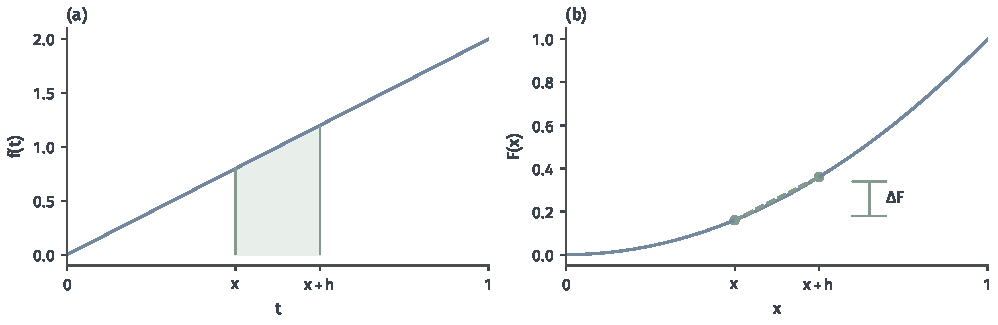
\includegraphics[width=169.0mm]{figures/01-mathematical-preliminaries-upper/01-mathematical-language-combinatorics-analysis-optimization/matplotlib/chapter3-concept-processes/accumulation-increment.pdf}
 \caption{(a) $f(t)=2t$在$[x,x+h]$上的绿色面积。(b) $F(x)=x^2$对应的增量$\Delta F$。图取$x=0.4,h=0.2$，两者都等于$0.2$。将增量除以$h$得到短区间平均值；只有再令$h\to0$，它才趋于$f(x)$，不能把有限平均值直接当作基点导数。}
 \label{fig:analysis-process-accumulation-increment}
\end{figure*}

\subsubsection{导数的积分}

现在改为先给定$G$，再计算其导数的积分，目标是恢复端点变化。
连续导数提供最直接的充分条件，导数仅黎曼可积时仍可恢复；若只知道几乎处处可导且导数勒贝格可积，还需要对$G$的整体变化加条件。

\paragraph{黎曼可积导数的基本定理}
中值定理把每段端点增量写成导数取样值乘区间长度，因此端点恢复的关键是这些取样和能否趋于积分，而不必要求导数连续。
下面先给出黎曼可积导数的结论；连续导数是其中自动满足可积性的特例。
\begin{theorem}[黎曼可积导数的端点公式]
\label{thm:analysis-riemann-derivative-ftc}
\label{thm:analysis-newton-leibniz-continuous}
设$G$在$[a,b]$上连续、在$(a,b)$上可导，且存在黎曼可积函数$g:[a,b]\to\mathbb R$在内点满足$g=G'$。
则
\[
 \int_a^bg(x)\,\mathrm dx=G(b)-G(a).
\]
端点处给$g$指定的有限值不影响积分。特别地，若$G\in C^1([a,b])$，可取$g=G'$。
上述黎曼积分也等于相应的勒贝格积分。
\end{theorem}
\begin{proof}
对任意分割，在每个小区间上用中值定理选$\xi_i$，得到
\[
 G(b)-G(a)=\sum_i\bigl(G(x_i)-G(x_{i-1})\bigr)
 =\sum_i g(\xi_i)(x_i-x_{i-1}).
\]
$g$黎曼可积保证任意细分割的这些取样和都趋于$\int_a^bg$，所以等式成立。
改变两个端点的值仍保持黎曼可积且不改变积分。若$G\in C^1([a,b])$，连续函数的黎曼可积性保证可选$g=G'$；两种积分的一致性由定理~\ref{thm:analysis-riemann-lebesgue-consistency}给出。
\end{proof}
例如$G(x)=x^3/3$在$[0,1]$上连续可微，$G'(x)=x^2$，故$\int_0^1x^2\,\mathrm dx=1/3$，与图~\ref{fig:analysis-process-riemann-upper-lower}中上下和夹住的数值一致。
这一定理是后面计算具体积分的主要工具：先找一个原函数，再取两端的差。

\paragraph{康托尔函数的反例}
几乎处处可导只记录零测例外之外的局部变化，未必记录全部端点变化。第~\ref{sec:analysis-cantor-function}节的康托尔函数给出具体反例。
\begin{example}[康托尔函数的导数积分不恢复端点差]
\label{ex:analysis-cantor-ftc-failure}
设$F:[0,1]\to[0,1]$为康托尔函数，$C$为康托尔集。由第~\ref{sec:analysis-cantor-function}节，$F$连续、非减，$F(0)=0$、$F(1)=1$，并且在构造中删去的每个开区间上为常数。这些开区间的并就是$[0,1]\setminus C$，所以在零测集$C$之外，$F'=0$。
在导数未定义的点上令$F'=0$，所得函数几乎处处为零、勒贝格可积，于是
\[
 F(1)-F(0)=1,\qquad \int_0^1F'(x)\,\mathrm dx=0.
\]
\end{example}
所以“连续、几乎处处可导、导数可积”三项合在一起，仍不足以由导数的积分恢复函数。缺少的条件正是该节已经验证不成立的绝对连续性：康托尔函数的全部增长集中在总长度可以任意小的区间族上。

\paragraph{绝对连续函数的导数基本定理}
康托尔函数说明，连续性不能排除集中在零测集上的整体变化，因而需要更强的条件。
定义~\ref{def:measurable-absolutely-continuous-function}的绝对连续条件控制许多短区间上的总变化，能排除导数遗漏整体变化的情形。
\begin{theorem}[绝对连续函数的导数积分]
\label{thm:measurable-absolute-continuity-ftc}
若$G:[a,b]\to\mathbb R$绝对连续，则$G'$几乎处处存在，并有实值勒贝格可积函数$g$与$G'$几乎处处相等，使每个$x\in[a,b]$满足
\begin{equation}
 G(x)=G(a)+\int_a^xg(t)\,\mathrm dt.
\label{eq:measurable-absolute-continuity-representation}
\end{equation}
特别地，$G(b)-G(a)=\int_a^bG'(t)\,\mathrm dt$，其中在未定义导数的零测例外上可取值零；这些积分为勒贝格积分。
\end{theorem}
定理从绝对连续性同时推出三件事：导数几乎处处存在，导数可积，导数的积分恢复端点变化。这是测度论的基本结论，这里引用而不证明，完整证明见教材\scite{math-folland1999real}。

另一个方向已在定理~\ref{thm:analysis-lebesgue-primitive-derivative}中直接证明：勒贝格可积函数的累计必绝对连续，且几乎处处以被积函数为导数。
合看两个方向，在$[a,b]$上，$F$绝对连续当且仅当存在勒贝格可积函数$g$使
$F(x)=F(a)+\int_a^xg(t)\,\mathrm dt$，此时$F'=g$几乎处处。
所以绝对连续恰好刻画了能由导数积分恢复的函数；示例~\ref{ex:analysis-cantor-ftc-failure}则说明一致连续还不够。

\paragraph{局部Lipschitz连续函数的导数基本定理}
Lipschitz条件直接控制函数的变化，由它可以得到绝对连续，从而保证导数几乎处处存在，并在闭区间上由导数积分恢复总变化。\term{Rademacher定理}（Rademacher theorem）说明，不可导的例外点只占零测集。
\begin{theorem}[一维Rademacher定理]
\label{thm:measurable-rademacher}
若$U\subseteq\mathbb R$为开集，$f:U\to\mathbb R$局部Lipschitz连续，则$f'$在$U$内几乎处处存在且有限。若$f$在某个开区间上具有Lipschitz常数$L$，则该区间内导数存在的点满足$|f'|\leq L$。
\end{theorem}
证明先在紧区间上用绝对连续函数的基本定理得到导数存在，再用可数覆盖把局部结论合并到整个开集。
\label{sec:analysis-rademacher-proof}
\begin{proof}
紧区间上具有Lipschitz常数$L$的函数绝对连续：给定$\varepsilon>0$，取$\delta=\varepsilon/L$即可（$L=0$时函数为常数）。基本定理便保证它几乎处处可导。若$f$只在开集$U$上局部Lipschitz，可选取可数多个端点为有理数的闭区间，使其内部覆盖$U$，并使每个区间都包含在某个具有Lipschitz常数的邻域内。
各区间上的不可导点集为零测集，它们的可数并仍为零测集，故$f'$在$U$内几乎处处存在。导数存在的点处，对Lipschitz差商界取极限便给出$|f'|\leq L$。
\end{proof}
绝对值函数在原点的左右导数不同，仍符合上述几乎处处结论；定理没有把尖点处的左右导数合成一个经典导数。

在闭区间$[a,b]$上具有Lipschitz常数的函数$G$绝对连续，因此其导数除几乎处处存在之外，还满足$G(b)-G(a)=\int_a^bG'(t)\,\mathrm dt$。
康托尔函数连续、几乎处处可导且导数可积，却不满足这一公式，因此它不是Lipschitz函数。可见Lipschitz条件是一种便于验证、足以排除这类反例的条件。

\subsection{积分的运算法则}
\label{sec:analysis-integral-calculus-rules}

从这里起，本章后续的积分一律采用勒贝格积分；“可积”指绝对值的积分有限，非负函数的积分则允许为无穷。
前面已经证明积分的基本性质，现在说明怎样用它们计算函数的加减、范围的分拆，以及换元积分与分部积分。
以下$E,A,B$均为可测集，积分关于勒贝格测度。

\subsubsection{积分的基本运算}

函数相加与积分范围相加是不同的操作，分别由线性和区域可加性保证。
计算时先检查可测性及绝对可积性，再使用相应的等式；正负无穷不能通过移项抵消。

\paragraph{和的积分}
在同一可测集$E$上，若实值函数$f,g$均可积，则$|f+g|\leq|f|+|g|$保证$f+g$可积。
定理~\ref{thm:analysis-signed-integral-properties}给出
\[
 \int_E(f+g)\,\mathrm dm=\int_Ef\,\mathrm dm+\int_Eg\,\mathrm dm.
\]
反过来，同一范围上的两个有限积分也可以合并为和的积分。

\paragraph{差的积分}
两个可积函数的差仍可积，因为$|f-g|\leq|f|+|g|$。同一线性定理给出
\[
 \int_E(f-g)\,\mathrm dm=\int_Ef\,\mathrm dm-\int_Eg\,\mathrm dm.
\]
这里两项都是有限实数，不涉及正负无穷的相减。

\paragraph{数乘的积分}
把被积函数乘以固定实数$c$，积分也乘以$c$。若$f$可积，则$cf$可积，且
\[
 \int_Ecf\,\mathrm dm=c\int_Ef\,\mathrm dm.
\]
这仍是定理~\ref{thm:analysis-signed-integral-properties}的特例；$c=0$时两侧都为零。

\paragraph{积的积分}
乘积需要另行检查可积性，不能直接套用线性。若$f$可积、$g$可测且$|g|\leq M$几乎处处，其中$M$为有限常数，则$|fg|\leq M|f|$保证$fg$可积。
但即使$f,g,fg$都可积，也不能把乘积的积分拆成两个积分相乘：例如在$[0,1]$上取$f(x)=g(x)=x$，则$\int_0^1fg=1/3$，而$(\int_0^1f)(\int_0^1g)=1/4$。

\paragraph{不交范围的积分}
同一函数在不同范围上的累计，可以用区域可加性分拆。
若$A\cap B=\varnothing$，且$f$在$A\cup B$上可积，则定理~\ref{thm:analysis-integral-set-additivity}给出
\[
 \int_{A\cup B}f\,\mathrm dm=\int_Af\,\mathrm dm+\int_Bf\,\mathrm dm.
\]
这与“和的积分”不同：这里改变的是积分范围，被积函数没有相加。取$A=[a,c]$、$B=(c,b]$，便得到区间记号下的$\int_a^bf=\int_a^cf+\int_c^bf$。

\paragraph{重叠范围的积分}
若两个范围重叠，分别累计会把交集计算两次，需要减去一次。
对在$A\cup B$上可积的$f$，有
\[
 \int_{A\cup B}f\,\mathrm dm
 =\int_Af\,\mathrm dm+\int_Bf\,\mathrm dm-\int_{A\cap B}f\,\mathrm dm.
\]
将$A\cup B$拆成$A\setminus B$、$A\cap B$、$B\setminus A$三个不交部分，再用区域可加性即可得到此式。

\paragraph{差集上的积分}
从可测范围$A$中去掉可测子集$B\subseteq A$时，去掉的累计量正是$B$上的积分。
若$f$在$A$上可积，由$A=(A\setminus B)\cup B$的不交分拆，得到
\[
 \int_{A\setminus B}f\,\mathrm dm=\int_Af\,\mathrm dm-\int_Bf\,\mathrm dm.
\]

\paragraph{积分的比较}
被积函数几乎处处的大小关系可以传给积分。若$f,g$可积且$f\leq g$几乎处处，则
\[
 \int_Ef\,\mathrm dm\leq\int_Eg\,\mathrm dm.
\]
这是因为$g-f$几乎处处非负且可积，其积分非负，再由差的积分公式移项即可。

\paragraph{积分的绝对值界}
累计中的正负抵消不会超过绝对值的累计。由$-|f|\leq f\leq|f|$及积分的比较得到
\[
 \left|\int_Ef\,\mathrm dm\right|\leq\int_E|f|\,\mathrm dm.
\]
此处$f$可积，所以不等式两侧均有限。

\paragraph{积分的误差估计}
将绝对值界用于两个可积函数之差，就能控制积分结果的误差：
\[
 \left|\int_Ef\,\mathrm dm-\int_Eg\,\mathrm dm\right|
 \leq\int_E|f-g|\,\mathrm dm.
\]
若进一步有$m(E)<\infty$且$|f-g|\leq\eta$几乎处处，则右侧不超过$\eta\,m(E)$。
后面讨论极限与积分时，将用这一估计把函数的共同误差转成积分误差。

\subsubsection{换元积分法}
\label{sec:analysis-coordinate-change-integral-applications}

变量替换既改变函数的表达，也改变输入集合的长度，导数的绝对值负责一维长度的缩放。
下面先给出一一对应换元的一般结论，再说明计算中常用的端点写法，最后用几个例子展示完整步骤。

\paragraph{可测函数的换元公式}
对非负函数，换元要保留全部累计；对有符号函数，还需保证正负部分都有限。
下面用微分同胚条件同时控制可逆性、可测性与局部长度变化。
\begin{theorem}[一维勒贝格积分的换元公式]
\label{thm:analysis-lebesgue-change-variables}
设$I,J\subseteq\mathbb R$为开区间，$T:I\to J$是$C^1$微分同胚，即$T$双射且$T,T^{-1}$连续可微。
对非负勒贝格可测$g:J\to[0,\infty]$，有
\[
 \int_Jg(u)\,\mathrm du=\int_Ig(T(x))|T'(x)|\,\mathrm dx,
\]
允许两边为无穷。若$g:J\to\mathbb R$可测，则$g$在$J$上可积当且仅当$g\circ T\,|T'|$在$I$上可积，此时同一等式给出有限积分值。
\end{theorem}
直观上，$T$把输入中长为$\Delta x$的小区间映成长约$|T'(x)|\Delta x$的小区间，因子$|T'(x)|$记录这种长度缩放。
一般换元定理的证明先把这种局部长度关系推广到可测集合，再经简单函数及单调逼近推广到非负函数；这里引用这一结论\scite{math-folland1999real}。
有符号版本则先对$|g|$换元，确认两侧同时绝对可积，再分别对正负部分换元。
由于单点的测度为零，$I,J$取开区间还是闭区间不影响积分值。

\paragraph{端点形式的换元}
定理中的等式不带方向：右侧乘$|T'|$，左侧按像区间从左到右累计。计算时更常写成端点形式，不必先判断$T$是递增还是递减。
设$T$在开区间$(a,b)$上是$C^1$微分同胚，并连续延拓到两端，$g$在像区间上非负可测或可积。微分同胚的导数处处非零（否则反函数在对应点不可导），又是连续函数，所以不变号，$T$严格单调。
若$T$递增，则$|T'|=T'$，像区间从$T(a)$到$T(b)$，定理直接给出
\[
 \int_{T(a)}^{T(b)}g(u)\,\mathrm du=\int_a^bg(T(x))T'(x)\,\mathrm dx.
\]
若$T$递减，则$|T'|=-T'$，像区间从$T(b)$到$T(a)$，定理给出$\int_{T(b)}^{T(a)}g(u)\,\mathrm du=-\int_a^bg(T(x))T'(x)\,\mathrm dx$；按有向端点约定把左侧改写为$-\int_{T(a)}^{T(b)}g$，两边的负号抵消，得到与递增情形完全相同的式子。
因此端点形式对两种单调方向统一成立：导数$T'$的符号与端点的先后共同记录了方向。

\paragraph{换元的计算示例}
下面三个例子依次检验递增换元、递减换元，以及用三角函数消去根式的换元。每个例子都先核对微分同胚条件，再使用端点形式。
\begin{example}[用递增换元计算指数型积分]
计算$\int_0^12xe^{x^2}\,\mathrm dx$。被积函数形如$g(T(x))T'(x)$，其中$T(x)=x^2$、$g(u)=e^u$。
在开区间$(0,1)$上，$T'(x)=2x>0$，反函数$T^{-1}(u)=\sqrt u$在$(0,1)$上连续可微，所以$T:(0,1)\to(0,1)$是$C^1$微分同胚。
注意$T'(0)=0$，$T$不能在包含$0$的开区间上作为微分同胚；这里只在$(0,1)$上换元，端点的单点不影响积分。
端点形式给出
\[
 \int_0^12xe^{x^2}\,\mathrm dx=\int_{T(0)}^{T(1)}e^u\,\mathrm du=\int_0^1e^u\,\mathrm du.
\]
最后用定理~\ref{thm:analysis-riemann-derivative-ftc}，取原函数$e^u$，得到$e^1-e^0=e-1$。
\end{example}

导数为负时，端点的先后顺序会颠倒，端点形式自动处理由此产生的符号。
\begin{example}[用递减换元计算三角函数积分]
计算$\int_0^{\pi/2}\sin x\cos^2x\,\mathrm dx$。取$T(x)=\cos x$，它在$(0,\pi/2)$上满足$T'(x)=-\sin x<0$，是到$(0,1)$的递减$C^1$微分同胚，反函数$\arccos$在$(0,1)$上连续可微。
按端点形式，
\[
 \int_0^{\pi/2}\cos^2x\,(-\sin x)\,\mathrm dx=\int_{T(0)}^{T(\pi/2)}u^2\,\mathrm du=\int_1^0u^2\,\mathrm du=-\frac13,
\]
所以$\int_0^{\pi/2}\sin x\cos^2x\,\mathrm dx=1/3$。
若直接使用定理的无方向形式，则$|T'(x)|=\sin x$，原积分等于$\int_{(0,1)}u^2\,\mathrm du=1/3$，结果相同。
\end{example}
两种写法的差别只在方向记在哪里：端点形式记在端点的先后中，无方向形式记在$|T'|$中。

换元还可以把不易直接找原函数的积分化为容易计算的形式。
\begin{example}[用正弦换元计算四分之一单位圆的面积]
单位圆在第一象限部分的面积是
\[
 \int_0^1\sqrt{1-x^2}\,\mathrm dx.
\]
令$x=T(\theta)=\sin\theta$，则$T:(0,\pi/2)\to(0,1)$递增，$T'(\theta)=\cos\theta>0$，反函数$\arcsin$在$(0,1)$上连续可微。
在$(0,\pi/2)$上$\cos\theta>0$，所以$\sqrt{1-\sin^2\theta}=\cos\theta$，从而
\[
 \int_0^1\sqrt{1-x^2}\,\mathrm dx
 =\int_0^{\pi/2}\sqrt{1-\sin^2\theta}\,\cos\theta\,\mathrm d\theta
 =\int_0^{\pi/2}\cos^2\theta\,\mathrm d\theta.
\]
由$\cos^2\theta=(1+\cos2\theta)/2$，原函数可取$\theta/2+\sin(2\theta)/4$，代入两端得到$\pi/4$。
\end{example}
这里换元的方向是把原积分写成定理右侧的形式：先确定新旧变量的对应及导数，再化简被积函数；开方时必须用到$\cos\theta$在所取区间上的符号。

\subsubsection{分部积分法}
\label{sec:analysis-integration-remainders}

乘积的导数$(uv)'=u'v+uv'$含有两项。对它积分并使用绝对连续函数的端点恢复公式，就能把其中一项的积分移到等式另一侧。
下面直接使用绝对连续条件；连续可微函数是其特例。

\paragraph{分部积分公式}
绝对连续保证导数几乎处处存在、可积且记录全部增量，因此可以对乘积的求导公式积分。
只知道几乎处处可导仍不充分，示例~\ref{ex:analysis-cantor-ftc-failure}已说明这一差别。
\begin{theorem}[勒贝格积分的分部积分公式]
\label{thm:analysis-lebesgue-integration-by-parts}
若$u,v:[a,b]\to\mathbb R$绝对连续，则$uv$绝对连续，$uv'$与$u'v$可积，且
\begin{equation}
 \int_a^bu(x)v'(x)\,\mathrm dx
 =[u(x)v(x)]_a^b-\int_a^bu'(x)v(x)\,\mathrm dx.
\label{eq:analysis-integration-by-parts}
\end{equation}
导数在零测例外上的可测有限取值不影响结果。
\end{theorem}
\begin{proof}
$u,v$连续且有界，导数可积，所以$uv'$与$u'v$可积。
对有限个两两不交区间，有
\[
 \begin{aligned}
 \sum_j|u(b_j)v(b_j)-u(a_j)v(a_j)|
 &\leq\|u\|_\infty\sum_j|v(b_j)-v(a_j)|\\
 &\quad+\|v\|_\infty\sum_j|u(b_j)-u(a_j)|.
 \end{aligned}
\]
两因子的绝对连续性使右侧随区间总长度趋零，故$uv$绝对连续。
在两导数都存在的点，$(uv)'=u'v+uv'$；将绝对连续函数的端点恢复定理用于$uv$，再用有限线性移项，便得公式。
\end{proof}
使用公式时，要把被积函数拆成一个因子$u$与另一个因子的导数$v'$：求导后变简单的因子取作$u$，容易找到原函数的因子取作$v'$。

\paragraph{分部积分的计算示例}
下面三个例子分别说明怎样选取$u$与$v'$：让多项式因子求导降次，把单个因子看成与常数一的乘积，以及选择不当会使积分变复杂。
\begin{example}[多项式乘指数函数的分部积分]
计算$\int_0^1xe^x\,\mathrm dx$。取$u(x)=x$、$v'(x)=e^x$，则$u'(x)=1$，可取$v(x)=e^x$；两者都在$[0,1]$上连续可微，因而绝对连续。公式给出
\[
 \int_0^1xe^x\,\mathrm dx=[xe^x]_0^1-\int_0^1e^x\,\mathrm dx
 =(e-0)-(e-1)=1.
\]
\end{example}
这里$x$求导后变成常数，剩下的积分可以直接由原函数计算。

被积函数只有一个因子时，可以把常数一当作另一个因子。
\begin{example}[把对数函数看成与常数一的乘积]
计算$\int_1^e\log x\,\mathrm dx$。把被积函数写成$\log x\cdot1$：取$u(x)=\log x$、$v'(x)=1$，则$u'(x)=1/x$，可取$v(x)=x$；两者都在$[1,e]$上连续可微。于是
\[
 \int_1^e\log x\,\mathrm dx=[x\log x]_1^e-\int_1^e\frac1x\cdot x\,\mathrm dx
 =e-(e-1)=1.
\]
\end{example}
对数的导数是有理函数，分部积分正好消去了难以直接积分的对数。

因子的分配也可能使计算变繁，下面的例子比较两种选法。
\begin{example}[因子的分配决定计算是否简化]
计算$\int_0^\pi x\sin x\,\mathrm dx$。取$u(x)=x$、$v'(x)=\sin x$，则$u'(x)=1$，可取$v(x)=-\cos x$，于是
\[
 \int_0^\pi x\sin x\,\mathrm dx=[-x\cos x]_0^\pi+\int_0^\pi\cos x\,\mathrm dx
 =\pi+[\sin x]_0^\pi=\pi.
\]
若反过来取$u=\sin x$、$v'=x$，则$v=x^2/2$，剩下的积分变为$\int_0^\pi x^2\cos x/2\,\mathrm dx$，比原积分更复杂。
\end{example}
在无穷区间上使用公式时，先对有限截断应用公式，再分别核查边界项的极限以及两个被积项的绝对可积性，不能无故删除端点项。

\paragraph{Taylor公式的积分余项}
分部积分的一个重要应用，是把Taylor公式中的余项写成一个确定的积分。
第~\ref{sec:analysis-taylor-approximation}节的Lagrange余项$f^{(r+1)}(\xi)h^{r+1}/(r+1)!$中，$\xi$只知道位于两端之间，具体位置未知。
若$f^{(r+1)}$连续，可以从端点公式$f(x_0+h)-f(x_0)=\int_{x_0}^{x_0+h}f'(t)\,\mathrm dt$出发，每做一次分部积分就从积分中分出Taylor多项式的一项；剩下的积分就是余项本身，不含未知点，可以直接计算或估计。

设$f$在包含以$x_0$、$x_0+h$为端点的闭区间的某个开区间上$r+1$阶连续可微，其中$r$为非负整数。为了同时处理正、负$h$，令$\phi(t)=f(x_0+th)$，$t\in[0,1]$；链式法则给出$\phi^{(k)}(t)=h^kf^{(k)}(x_0+th)$。
第一步由黎曼可积导数的端点公式得到
\[
 \phi(1)-\phi(0)=\int_0^1\phi'(t)\,\mathrm dt.
\]
对$k\geq1$，在
$\int_0^1\frac{(1-t)^{k-1}}{(k-1)!}\phi^{(k)}(t)\,\mathrm dt$中取$u=\phi^{(k)}$、$v=-(1-t)^k/k!$，则$v'=(1-t)^{k-1}/(k-1)!$，而$v(1)=0$、$v(0)=-1/k!$。分部积分给出
\[
 \int_0^1\frac{(1-t)^{k-1}}{(k-1)!}\phi^{(k)}(t)\,\mathrm dt
 =\frac{\phi^{(k)}(0)}{k!}
 +\int_0^1\frac{(1-t)^k}{k!}\phi^{(k+1)}(t)\,\mathrm dt.
\]
从$k=1$用到$k=r$，每一步分出一项$\phi^{(k)}(0)/k!=f^{(k)}(x_0)h^k/k!$，便得
\begin{equation}
 f(x_0+h)=\sum_{k=0}^r\frac{f^{(k)}(x_0)}{k!}h^k
 +\frac{h^{r+1}}{r!}
   \int_0^1(1-t)^r f^{(r+1)}(x_0+th)\,\mathrm dt.
\label{eq:analysis-taylor-integral-remainder}
\end{equation}
最后一项称为Taylor公式的积分余项。这里的余项是勒贝格积分，$f^{(r+1)}$连续保证被积函数在$[0,1]$上可积。
若$|f^{(r+1)}|\leq M$，积分权重$(1-t)^r/r!$的总量为$1/(r+1)!$，故余项不超过$M|h|^{r+1}/(r+1)!$，与Lagrange余项的估计一致。

积分余项不含未知点，对具体函数可以直接算出或夹逼。先看三阶导数为常数的立方函数。
\begin{example}[立方函数的积分余项]
取$f(x)=x^3-3x$、$r=2$。由于$f'''\equiv6$，对任意$x_0$和$h$，积分余项为
\[
 \frac{h^3}{2!}\int_0^1 6(1-t)^2\,\mathrm dt=\frac{h^3}{2}\cdot6\cdot\frac13=h^3.
\]
这与第~\ref{sec:analysis-taylor-approximation}节中$x_0=1/2$处的完整展开相同：三阶Taylor多项式之外没有剩余项，二阶多项式的误差恰为$h^3$。
\end{example}

被积函数不是常数时，可以用它的上下界夹住余项，得到截断误差的范围。
\begin{example}[用积分余项估计$e$]
取$f(x)=e^x$、$x_0=0$、$h=1$。各阶导数都是$e^x$，式~\eqref{eq:analysis-taylor-integral-remainder}给出
\[
 e=\sum_{k=0}^r\frac1{k!}+\frac1{r!}\int_0^1(1-t)^re^t\,\mathrm dt.
\]
由$1\leq e^t\leq e$及$\int_0^1(1-t)^r\,\mathrm dt=1/(r+1)$，余项介于$1/(r+1)!$与$e/(r+1)!$之间。
例如$r=3$时，三阶Taylor多项式在$h=1$处的值为$1+1+1/2+1/6=8/3\approx2.6667$，余项$e-8/3\approx0.0516$，确实落在$1/24\approx0.0417$与$e/24\approx0.1133$之间。
\end{example}



\subsection{函数列的极限}
\label{sec:measurable-convergence-and-integrals}
\label{sec:analysis-limit-integral-interchange}
\label{sec:analysis-function-convergence-essential-bounds}

设一列函数$f_n$趋于$f$。仅知道每个位置的函数值趋近，还不能判断极限函数是否连续、是否可微，也不能判断积分的极限是否等于极限函数的积分。
这三个问题控制的对象不同：连续性比较邻近输入的函数值，微分比较差商，积分比较全部范围上的累计。
下面先明确收敛方式，再分别回答极限与连续、极限与微分、极限与积分的关系；本小节涉及的积分全部为勒贝格积分。

\subsubsection{函数列的收敛方式、判别与关系}
\label{sec:analysis-convergence-mode-relations}

逐点收敛允许每个输入单独选择稳定时刻，一致收敛要求同一个下标控制全部输入，几乎处处收敛则允许在一个固定的零测范围上例外。
先区分这些条件，后面才能说明哪种控制足以保持哪种性质。

\paragraph{点态收敛}
固定一个输入以后，比较的只是一列实数。这里不需要函数可微或可积，函数值按实数的绝对值比较。
\begin{definition}[点态收敛]
\label{def:analysis-pointwise-almost-everywhere-convergence}
设$X\subseteq\mathbb R$，$f_n,f:X\to\mathbb{R}$。若
\[
 \begin{gathered}
  \forall x\in X,\quad
  \forall\varepsilon>0,\quad
  \exists N=N(x,\varepsilon)\in\mathbb N,\\
  \forall n\geq N,\quad
  |f_n(x)-f(x)|<\varepsilon,
 \end{gathered}
\]
即对每个$x$都有$\lim_n f_n(x)=f(x)$，称$f_n$点态收敛到$f$。点态收敛也称逐点收敛（pointwise convergence）。
\end{definition}
固定$x$以后，点态收敛就是已经定义的数列收敛；不同位置可以需要不同的起始下标。

\paragraph{点态收敛的判据}
若还不知道极限函数，可以对每个固定输入使用实数列的柯西收敛准则。
这时各输入仍可各自选择尾部起点，不要求同一个下标适用于全部输入。
\begin{theorem}[函数列点态收敛的柯西判据]
\label{thm:analysis-pointwise-cauchy-criterion}
设$X$非空，$f_n:X\to\mathbb R$。存在$f:X\to\mathbb R$使$f_n$点态收敛到$f$，当且仅当
\[
 \begin{gathered}
 \forall x\in X,\quad\forall\varepsilon>0,\quad
 \exists N=N(x,\varepsilon)\in\mathbb N,\\
 \forall m,n\geq N,\quad |f_m(x)-f_n(x)|<\varepsilon.
 \end{gathered}
\]
\end{theorem}
\begin{proof}
固定$x$，若$f_n(x)$收敛，则实数列的柯西准则给出该条件。
反之，条件使每个$(f_n(x))_n$都是实数柯西列，故都有有限极限；定义$f(x)=\lim_nf_n(x)$，便得到所需的点态极限函数。
\end{proof}

\paragraph{一致收敛}
即使每个输入处的误差最终都很小，开始稳定的时刻仍可能依赖输入。
若希望选定一个下标后就同时控制全部输入，需要更强的一致条件。

\begin{definition}[函数列的一致收敛]
\label{def:analysis-uniform-convergence}
设$X\subseteq\mathbb R$非空，$f_n,f:X\to\mathbb R$。若
\[
  \forall\varepsilon>0,\quad
  \exists N=N(\varepsilon)\in\mathbb N,\quad
  \forall x\in X,\quad
  \forall n\geq N,\quad
  |f_n(x)-f(x)|<\varepsilon,
\]
就称$f_n$在$X$上一致收敛到$f$。等价地，
\begin{equation}
  \lVert f_n-f\rVert_{\infty}
  :=
  \sup_{x\in X}|f_n(x)-f(x)|
  \longrightarrow0.
\label{eq:analysis-uniform-convergence}
\end{equation}
这里的上确界检查全部输入，不排除任何位置；对一般函数，它可能等于$+\infty$，一致收敛要求这些误差最终有限并趋于零。
\end{definition}
两个定义只交换了“$\forall x$”与“$\exists N$”的次序：点态收敛先固定输入再选$N(x,\varepsilon)$，一致收敛先选$N(\varepsilon)$，再要求它适用于全部输入。
在图形上，以极限$f$为中心画出上下宽$\varepsilon$的误差带：一致收敛要求从某个下标起，$f_n$的整个图形都落在带内；点态收敛只要求每条竖线$x=x_0$上的点$f_n(x_0)$最终进入带内，进入的时刻可以随$x_0$改变。

图~\ref{fig:analysis-process-convergence-modes}用两个具体函数列比较这一差别，误差带都取$\varepsilon=0.12$。
(a)中$g_n(x)=x/n$在$[0,1]$上的最大误差为$1/n$，从$N=9$起整个图形都在带内，同一个$N$对全部输入适用。
(b)中$f_n(x)=x^n$在$[0,1)$上点态收敛到$0$：在$x_1=0.5$处从$n=4$起进入带内，在$x_2=0.9$处要等到$n=21$；输入越靠近$1$，所需的$N$越大。
每条$f_n$都在$x=\varepsilon^{1/n}<1$处离开误差带；由于$\sup_{[0,1)}x^n=1$，没有一个$N$能对全部输入同时适用。
\begin{figure*}[!htbp]
 \centering
 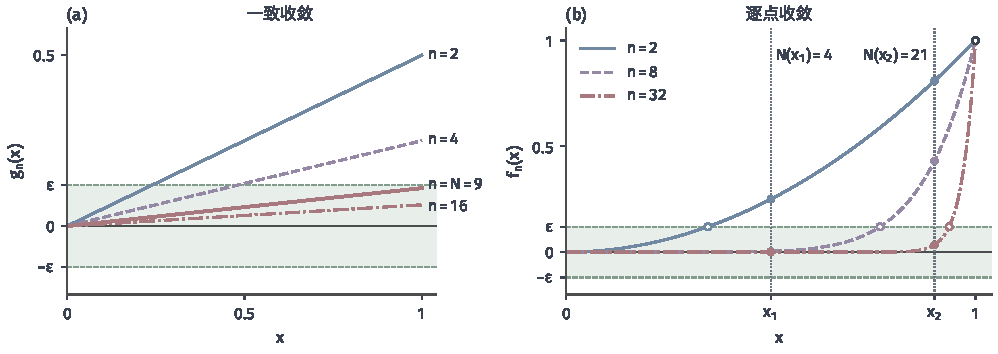
\includegraphics[width=169.0mm]{figures/01-mathematical-preliminaries-upper/01-mathematical-language-combinatorics-analysis-optimization/matplotlib/chapter3-concept-processes/convergence-modes.pdf}
 \caption{函数列的两种收敛方式，绿色带为极限$0$附近宽$\varepsilon=0.12$的误差带。(a)一致收敛：$g_n(x)=x/n$在$[0,1]$上的最大误差为$1/n$，$n=2,4$时图形超出误差带，从$N=9$起（图中加粗）整个图形都在带内。(b)逐点收敛：$f_n(x)=x^n$在$[0,1)$上趋于$0$，图绘$n=2,8,32$。竖虚线$x_1=0.5$、$x_2=0.9$上的实心点是各曲线在该处的值，进入误差带所需的下标分别为$N(x_1)=4$、$N(x_2)=21$；空心点标出各曲线离开误差带的位置$x=\varepsilon^{1/n}$，约为$0.35,0.77,0.94$。右端空心圆表示$x=1$不在定义域内。有限条曲线只示意定义中的量词次序，不代替收敛的证明。}
 \label{fig:analysis-process-convergence-modes}
\end{figure*}

\paragraph{一致收敛的判据}
若尚不知道候选极限，可以改为检查后面的函数是否彼此一致接近。
实数的完备性把各点极限组合为一个函数，共同误差再保证收敛一致。
\begin{theorem}[实值函数列的一致柯西判据]
\label{thm:analysis-uniform-cauchy-criterion}
设$X$非空、$f_n:X\to\mathbb R$。存在$f$使$f_n$在$X$上一致收敛，当且仅当
\[
 \forall\varepsilon>0,\quad\exists N,\quad
 \forall m,n\geq N,\quad\forall x\in X,\quad
 |f_m(x)-f_n(x)|<\varepsilon.
\]
\end{theorem}
\begin{proof}
若一致收敛，三角不等式把两项之差控制为它们到极限的两个一致误差之和，便得必要性。
反之，每个固定$x$处的实数列是柯西列，故有$f(x)=\lim_n f_n(x)$。
给定$\varepsilon>0$，先取$N$使$m,n\geq N$时对全部$x$有$|f_m(x)-f_n(x)|<\varepsilon/2$。
固定$n\geq N$并令$m\to\infty$，得到$|f(x)-f_n(x)|\leq\varepsilon/2$对全部$x$成立，所以收敛一致。
\end{proof}
此判据不要求各函数有界；若各$f_n$有界，极限与一个固定后项的共同误差有限，故极限也有界。

\paragraph{几乎处处收敛}
勒贝格积分不受零测修改的影响，因此可以允许函数列在一个固定的零测集上不收敛。
\begin{definition}[几乎处处收敛]
\label{def:analysis-almost-everywhere-convergence}
设$E\in\mathcal L(\mathbb R)$，$f_n,f:E\to\mathbb R$。若存在零测集$N_0\subseteq E$，使
\[
 \begin{gathered}
 \forall x\in E\setminus N_0,\quad
 \forall\varepsilon>0,\quad
 \exists N=N(x,\varepsilon),\\
 \forall n\geq N,\quad |f_n(x)-f(x)|<\varepsilon,
 \end{gathered}
\]
就称$f_n$几乎处处收敛到$f$。
\end{definition}
定义中的零测集$N_0$先于精度$\varepsilon$和下标选定，不能随$\varepsilon$或$n$改变；在它的补集上，函数列逐点收敛。
可数个零测例外可以先取并，合成一个共同的零测例外；不可数个零测集的并却未必零测。
若各$f_n$可测，几乎处处极限也可测，因为它与上极限$\limsup_nf_n$只在零测集上不同。

以下固定可测集$E\subseteq\mathbb R$及其上的可测实值函数$f_n,f$；点态与一致收敛本身只用到集合$E$，几乎处处收敛还依赖勒贝格测度给出的零测集。

\paragraph{三种收敛方式的关系}
定义~\ref{def:analysis-pointwise-almost-everywhere-convergence}、\ref{def:analysis-uniform-convergence}与\ref{def:analysis-almost-everywhere-convergence}的区别在于误差控制覆盖哪些点，以及是否允许共同的零测例外。
固定同一个极限函数，才能准确比较下面三种陈述。
\begin{theorem}[三种函数列收敛方式的关系]
\label{thm:analysis-convergence-mode-implications}
对上述函数列，有
\[
 f_n\text{一致收敛到}f
 \ \Longrightarrow\ f_n\text{点态收敛到}f
 \ \Longrightarrow\ f_n\text{几乎处处收敛到}f.
\]
两个逆命题一般都不成立；这些正向蕴含不要求$m(E)<\infty$。
\end{theorem}
\begin{proof}
一致收敛选出的$N(\varepsilon)$同时控制全部$x$，因而也控制任意一个固定的$x$，得到点态收敛。
点态收敛在每一点成立，可以在几乎处处收敛的定义中取空的例外集。
\end{proof}

若论证中对每个$n$另有零测例外集$N_n$，可先取可数并$N=\bigcup_nN_n$，得到一个适用于全部$n$的共同范围。
后面讨论函数项级数时，把$f_n$换成部分和函数列，以上关系同样适用。
下面两个例子分别说明这两个逆命题不成立。

\paragraph{点态收敛不保证一致收敛}
幂函数列在每个位置的误差最终都会变小，最大误差却始终为一。
\begin{example}[幂函数列点态收敛但不一致收敛]
\label{ex:analysis-power-not-uniform}
在$[0,1]$上取$f_n(x)=x^n$。它点态收敛到
\[
 f(x)=
 \begin{cases}
  0,&0\leq x<1,\\
  1,&x=1.
 \end{cases}
\]
每个固定的$0\leq x<1$都有$x^n\to0$；在端点$1$处，函数值与极限值始终都为$1$，误差为零。
但对每个$n$，$\sup_{x\in[0,1]}|f_n(x)-f(x)|=\sup_{0\leq x<1}x^n=1$，所以收敛不一致。
从量词看，固定$\varepsilon=1/2$后，无论选多大的$N$，在$n=N$时
总能选$x_N=(3/4)^{1/N}<1$，使误差$x_N^N=3/4>\varepsilon$。
\end{example}
失败的位置随$n$移动，正如图~\ref{fig:analysis-process-convergence-modes}(b)中离开误差带的空心点随$n$向$1$靠近；不能把“每个位置最终变小”改写成“某一轮以后所有位置都小”。
若把范围缩为$[0,a]$，其中$0\leq a<1$，则上确界误差为$a^n\to0$，同一列函数在这个范围上一致收敛。

若改把指定极限取为$g\equiv0$，同一列函数只是几乎处处收敛到$g$，在$x=1$处并不收敛到$g(1)=0$。
$f$与$g$几乎处处相等，却不是逐点相等的函数；比较收敛方式时不能省去这一差别。

\paragraph{几乎处处收敛不保证点态收敛}
几乎处处收敛不控制零测例外上的取值，那里的函数值可以发散。
\begin{example}[原点处发散而几乎处处趋零的函数列]
\label{ex:analysis-ae-not-pointwise}
在$[0,1]$上令$f_n(x)=n\mathbb I_{\{0\}}(x)$，并指定极限为零函数。
在每个$x\neq0$处，$f_n(x)=0$对全部$n$成立，所以函数列在零测集$\{0\}$之外收敛到零，即几乎处处趋零。
在$x=0$处，$f_n(0)=n\to\infty$，连有限的点态极限都不存在，所以$f_n$不点态收敛到零函数。
\end{example}
每个$f_n$都与零函数几乎处处相等；若把原点处的值全部改为零，所得的另一列函数便一致收敛到零。
所以零测改值不影响勒贝格积分，却可能改变原来这列函数的点态收敛和一致收敛：这两种收敛检查的是实际取值，不能只由几乎处处相等的关系决定。

\subsubsection{极限与连续}

逐点收敛只控制每个固定输入处的变化，不能统一控制邻近输入之间的差，因此不一定保留连续性。
一致收敛提供对全部输入共同有效的误差界，下面的定理说明这足以把连续性传给极限。
\begin{theorem}[一致极限保持连续性]
\label{thm:analysis-uniform-continuity-limit}
设$X\subseteq\mathbb R$，连续函数$f_n:X\to\mathbb R$一致收敛到$f$，则$f$在$X$上连续。
\end{theorem}
\begin{proof}
固定$a\in X$及$\varepsilon>0$，先选$N$使$\sup_X|f_N-f|<\varepsilon/3$，再由$f_N$在$a$处连续选$\delta$。当$x\in X$且$|x-a|<\delta$时，
\[
 |f(x)-f(a)|
 \leq |f(x)-f_N(x)|+|f_N(x)-f_N(a)|+|f_N(a)-f(a)|<\varepsilon.
\]
所以$f$连续。这里先固定一个对所有输入都适用的$N$，再调用单个$f_N$的连续性。
\end{proof}

示例~\ref{ex:analysis-power-not-uniform}中的幂函数列在$[0,1]$上的点态极限不连续，所以逐点收敛不能代替一致收敛。还需区分另一个逆向问题：若将同一函数列限制到$[0,1)$，点态极限是连续函数$0$，但$\sup_{[0,1)}x^n=1$，仍不一致趋零。因此极限连续也不能反推一致收敛。

局部一致收敛也足够：它指每个点都有一个相对邻域，使函数列在该邻域上一致收敛。把上述定理用于该邻域，即得极限在该点连续，因为检查某点的连续性只需用到它附近的输入。
局部一致收敛保留连续性，靠的是每点附近的共同误差尺度；几乎处处收敛的零测例外不能提供这种尺度。

\subsubsection{极限与微分}

求导比较的是输入尺度缩小后的差商，因此函数值一致接近仍可能漏掉快速振荡或尖点。先看快速振荡：函数值的一致收敛不能保证导数收敛。
\begin{example}[函数值一致趋零而导数不收敛]
\label{ex:analysis-oscillating-derivatives}
在$[0,2\pi]$上令$f_n(x)=\sin(nx)/n$。由$\sup|f_n|\leq1/n$，函数列一致趋于零函数，其导数恒为零。
另一方面，$f_n'(x)=\cos(nx)$。在$x=0$处$f_n'(0)=1$对全部$n$成立，不趋于极限函数的导数$0$；在$x=\pi$处$f_n'(\pi)=(-1)^n$，根本不收敛。
所以导数列$f_n'$连逐点趋于$0$都不成立。
\end{example}
函数值的振幅$1/n$趋零，但振荡频率$n$同时增大，两者相乘使导数的幅度始终为一。

一致极限甚至可能不可导：尖点可以由光滑函数一致逼近。
\begin{example}[光滑函数一致逼近绝对值函数]
\label{ex:analysis-smoothed-absolute-value}
对$\varepsilon>0$，令$f_\varepsilon(x)=\sqrt{x^2+\varepsilon^2}$，它在实轴上连续可微。由
\[
 0\leq f_\varepsilon(x)-|x|
 =\frac{\varepsilon^2}{\sqrt{x^2+\varepsilon^2}+|x|}\leq\varepsilon,
\]
$\varepsilon\downarrow0$时$f_\varepsilon$在实轴上一致趋于$|x|$，而极限在原点不可导。
各近似函数的导数为$f_\varepsilon'(x)=x/\sqrt{x^2+\varepsilon^2}$。对$x\neq0$，它趋于$\operatorname{sign}(x)$，其中正数的符号为$1$、负数的符号为$-1$；在原点，导数恒为零。
即使规定$\operatorname{sign}(0)=0$，导数的这种收敛也不一致：取$x_\varepsilon=\varepsilon^2$，则$f_\varepsilon'(x_\varepsilon)=\varepsilon/\sqrt{1+\varepsilon^2}\to0$，而$\operatorname{sign}(x_\varepsilon)=1$，误差趋于一。
\end{example}

因此要交换极限与求导，控制必须加在导数上。一种足够的控制是导数一致收敛并固定一个函数值；若只控制导数的积分误差，则得到绝对连续及几乎处处导数的结论，结论强度不同。

\paragraph{连续可微函数列导数的一致收敛}
若控制的是导数，还需固定一个函数值，才能排除任意的竖直平移。
\begin{theorem}[一致导数逼近与求导保持]
\label{thm:analysis-uniform-derivative-limit}
设$a<b$，$f_n\in C^1([a,b])$。若某个$x_0\in[a,b]$满足$f_n(x_0)\to c$，且$f_n'$在$[a,b]$上一致收敛到$g$，则$f_n$一致收敛到某个$f\in C^1([a,b])$，并有$f(x_0)=c$、$f'=g$。
\end{theorem}
\begin{proof}
对$f_n-f_m$使用中值定理，得到
\[
 |f_n(x)-f_m(x)|\leq |f_n(x_0)-f_m(x_0)|+(b-a)\lVert f_n'-f_m'\rVert_\infty.
\]
右侧随$m,n\to\infty$一致趋零，所以$f_n$一致柯西。实值函数列的一致柯西判据给出一致极限$f$，且$f(x_0)=c$。$f,g$均为连续函数的一致极限，因而连续。

还须证明$f'=g$。给定$\varepsilon>0$，取$N$使$n\geq N$时$\lVert f_n'-g\rVert_\infty<\varepsilon$。对$n,m\geq N$及$x\neq y$，中值定理给出
\[
 |(f_n-f_m)(y)-(f_n-f_m)(x)|\leq2\varepsilon|y-x|.
\]
固定$n\geq N$，令$m\to\infty$，再除以$|y-x|$，可知$f$与$f_n$的差商相差至多$2\varepsilon$。因此
\[
 \begin{aligned}
 \left|\frac{f(y)-f(x)}{y-x}-g(x)\right|
 &\leq2\varepsilon+
 \left|\frac{f_n(y)-f_n(x)}{y-x}-f_n'(x)\right|\\
 &\quad+|f_n'(x)-g(x)|.
 \end{aligned}
\]
先固定这个$n$再令$y\to x$，中间一项趋零，最后一项小于$\varepsilon$。由$\varepsilon$任意，得到$f'(x)=g(x)$；端点使用单侧差商。
\end{proof}
两个条件都不能省去。若没有单点收敛条件，$f_n(x)=n$的导数虽全为零，函数值却不收敛；若只有函数值一致收敛，示例~\ref{ex:analysis-oscillating-derivatives}和示例~\ref{ex:analysis-smoothed-absolute-value}已经说明求导可能失败。这个证明只用中值定理与一致柯西条件，不要求先把函数值写成导数的积分。

\paragraph{绝对连续函数列导数按积分误差的收敛}
导数未必一致收敛，但若导数绝对误差的总累计趋零，仍能控制所有端点之间的函数增量。
下面用勒贝格积分给出这一条件，结论不额外承诺极限导数连续。
\begin{theorem}[导数积分误差控制的极限]
\label{thm:analysis-integral-derivative-limit}
设$f_n$在$[a,b]$上绝对连续，$g$勒贝格可积，且某个$x_0\in[a,b]$满足$f_n(x_0)\to c$。
若
\[
 \int_a^b|f_n'(t)-g(t)|\,\mathrm dt\longrightarrow0,
\]
则$f_n$一致收敛到绝对连续函数$f(x)=c+\int_{x_0}^xg(t)\,\mathrm dt$，且$f'=g$几乎处处。
\end{theorem}
\begin{proof}
绝对连续函数的基本定理给出$f_n(x)=f_n(x_0)+\int_{x_0}^xf_n'(t)\,\mathrm dt$，因而
\[
 \sup_{x\in[a,b]}|f_n(x)-f(x)|
 \leq|f_n(x_0)-c|+\int_a^b|f_n'-g|\,\mathrm dt\longrightarrow0.
\]
可积函数的累计绝对连续，且导数几乎处处等于$g$，故得结论。
\end{proof}
导数一致收敛的定理给出$C^1$极限；这里的积分误差条件只保证绝对连续和几乎处处求导。

\subsubsection{极限与积分}

积分要控制的是整个范围上的累计。逐点误差变小，未必排除越来越窄的高峰，也未必排除向更远处移动的贡献。
可测函数列的上下极限及几乎处处极限仍可测，这已在第~\ref{sec:analysis-measurable-functions}节说明，所以极限函数总具备积分的资格。
下面比较四种条件：有限测度上的一致收敛、非负单调收敛、只有非负性时的单向估计，以及共同可积上界下的积分交换。

\paragraph{逐点收敛的反例}
每个输入处的误差趋零，未必排除面积集中的窄峰。下面固定峰的形状，比较总面积趋零与总面积保持不变两种情形。
\begin{example}[连续尖峰逐点趋零而积分不趋零]
\label{ex:analysis-continuous-spikes}
记$t_+=\max\{t,0\}$，在$[0,1]$上令
\begin{equation}
 b_n(x)=(1-|2nx-1|)_+,\qquad a_n(x)=2n\,b_n(x),\qquad n\geq1.
\label{eq:measurable-continuous-spikes}
\end{equation}
两列函数都连续，只可能在$[0,1/n]$上非零，顶点位于$1/(2n)$，高度分别为$1$和$2n$。
固定$x>0$后，充分大的$n$使$x>1/n$；在$x=0$处两列始终为零，所以它们都处处趋零。
由三角形面积公式，它们的勒贝格积分为
\[
 \int_0^1b_n\,\mathrm dx=\frac1{2n},\qquad \int_0^1a_n\,\mathrm dx=1.
\]
两列都不一致趋零，因为最大高度没有趋零。第一列的积分仍趋于零；第二列却有
\begin{equation}
 \int_0^1a_n(x)\,\mathrm dx=1,
 \qquad \int_0^1\lim_{n\to\infty}a_n(x)\,\mathrm dx=0.
\label{eq:analysis-continuous-spike-integral-failure}
\end{equation}
\end{example}
这个反例中各项和极限都可积，失败不在于积分没有定义，而在于逐点收敛没有控制面积的集中：峰的位置趋于$0$、宽度趋零，每个固定点最终都落在峰外，积分却始终保留整个面积。
下面先说明一致收敛在有限测度范围上能排除这种情形，再检查单调性和共同可积上界能否控制这项集中贡献。

\paragraph{有限测度上一致收敛下的积分极限}
\label{sec:analysis-classical-limit-integral}
一致误差乘总测度就控制了积分误差，因此一致收敛在有限测度范围上足以交换极限与积分。
这需要总测度有限，也需要各项确实可积。
\begin{theorem}[有限测度上的一致收敛与积分]
\label{thm:analysis-uniform-lebesgue-integral-limit}
设$E\in\mathcal L(\mathbb R)$，$m(E)<\infty$，实值可测函数$f_n$在$E$上可积，并在$E$上一致收敛到$f$。
则$f$可积，且
\begin{equation}
 \int_E|f_n-f|\,\mathrm dm
 \leq m(E)\|f_n-f\|_\infty\longrightarrow0,
 \qquad \int_Ef_n\,\mathrm dm\longrightarrow\int_Ef\,\mathrm dm.
\label{eq:analysis-uniform-riemann-limit}
\end{equation}
\end{theorem}
\begin{proof}
逐点极限$f$可测。一致收敛保证可选一个$n_0$使$\|f-f_{n_0}\|_\infty<1$，因此
$\int_E|f|\leq\int_E|f_{n_0}|+m(E)<\infty$。
对充分大的$n$，共同误差$\|f_n-f\|_\infty$有限，把它在$E$上积分即得所述绝对误差界；积分之差的绝对值不超过这项误差积分。
\end{proof}
总测度有限的条件不能删去，下面的例子把面积摊平到越来越长的区间上。
\begin{example}[无限测度上一致趋零而积分不变]
\label{ex:analysis-flattened-indicators}
在$\mathbb R$上令$f_n=n^{-1}\mathbb I_{[0,n]}$。由$\sup_{\mathbb R}|f_n|=1/n$，函数列一致趋于零函数；但每一项的积分为$n^{-1}m([0,n])=1$，而极限的积分为$0$。
\end{example}
因此，下面三项结论不再依赖有限测度和一致误差，改用单调性、非负性或共同可积上界控制总累计。

\paragraph{非负可测函数列的单调递增收敛}
记$f_n(x)\uparrow f(x)$表示每个固定$x$处的数列单调增加且趋于$f(x)$；允许忽略零测例外时，例外须包含在同一个零测集中。
规范简单逼近$s_n\uparrow f$正是这样逐步增加的。单调收敛定理回答定义非负积分时留下的问题：递增的非负可测函数列，其积分是否趋于极限函数的积分\scite{math-folland1999real}。
\begin{theorem}[单调收敛定理]
\label{thm:analysis-monotone-convergence}
设$E\in\mathcal L(\mathbb R)$，$f_n,f:E\to[0,\infty]$可测，且$f_n(x)\uparrow f(x)$几乎处处，则它们的勒贝格积分满足
\[   \lim_{n\to\infty}\int_E f_n\,\mathrm{d}m   =   \int_E f\,\mathrm{d}m. \]
两边都允许取$+\infty$。
\end{theorem}
\begin{proof}
把单调性或收敛关系失效的零测集并为$N$，并将$f_n$与$f$在$N$上都改为$0$。
修改后的函数仍可测且积分不变，所以可假定$f_n\uparrow f$逐点成立。由
$0\leq f_n\leq f$，积分序列单调不减且
\[   L:=\lim_{n\to\infty}\int_E f_n\,\mathrm{d}m   \leq\int_E f\,\mathrm{d}m. \]
还需证明反向不等式。任取满足$0\leq s\leq f$的简单函数，将它写为$s=\sum_{j=1}^m a_j\mathbb{I}_{E_j}$，其中$a_j>0$且$E_j$两两不交。固定$c\in(0,1)$，定义
\[   E_{j,n}   =   E_j\cap\{x:f_n(x)\geq ca_j\}. \]
由于$f_n\uparrow f$且$f\geq a_j$于$E_j$，有$E_{j,n}\uparrow E_j$。
第~\ref{sec:analysis-set-measure-continuity}节已由可数可加性证明测度对递增集合连续，
故$m(E_{j,n})\uparrow m(E_j)$。同时
\[   f_n   \geq   c\sum_{j=1}^m a_j\mathbb{I}_{E_{j,n}}, \]
从而
\[   L   \geq   \lim_{n\to\infty}   c\sum_{j=1}^m a_jm(E_{j,n})   =   c\int_E s\,\mathrm{d}m. \]
先令$c\uparrow1$，再对所有$0\leq s\leq f$的简单函数取上确界。根据非负积分的定义~\eqref{eq:analysis-nonnegative-lebesgue-integral}，$L\geq\int_E f\,\mathrm{d}m$。与前一不等式合并即得结论。
\end{proof}

非负性避免了正负无穷相消，单调性保证已经累计的贡献不会在后续消失。定理不要求存在可积的共同上界，也不要求各$\int f_n$有限。

回到示例~\ref{ex:analysis-finite-indicators-dirichlet}：有限点指示函数$d_n$递增到狄利克雷函数$d$，各项的勒贝格积分都为零，极限的积分为$m(Q_0)=0$，单调收敛定理的等式成立。黎曼积分在这里无法给出极限一侧的值，勒贝格积分则让这一逼近留在同一个积分框架内。
但非负递增不保证积分有限：在$(0,\infty)$上，$\mathbb I_{(0,n)}\uparrow1$，积分$n$增加到无穷，仍符合单调收敛等式。

\paragraph{非负可测函数列的下极限与积分估计}
若删去单调要求，只保留非负性，示例~\ref{ex:analysis-continuous-spikes}中的尖峰$a_n$说明积分等式可能失败，但仍有一个方向的不等式。对可能不收敛的函数列，可以用每个位置的下极限比较尾部的贡献。

\begin{lemma}[Fatou引理]
\label{lem:analysis-fatou}
设$E\in\mathcal L(\mathbb R)$。若$f_n:E\to[0,\infty]$可测，则
\begin{equation}
  \int_E\liminf_{n\to\infty}f_n\,\mathrm{d}m
  \leq
  \liminf_{n\to\infty}\int_Ef_n\,\mathrm{d}m.
\label{eq:analysis-fatou}
\end{equation}
\end{lemma}
\begin{proof}
令$g_n=\inf_{k\geq n}f_k$。则$g_n$可测，$0\leq g_n\uparrow\liminf_k f_k$。由单调收敛定理，
\[   \int_E\liminf_k f_k\,\mathrm{d}m   =   \lim_{n\to\infty}\int_E g_n\,\mathrm{d}m. \]
对每个$k\geq n$都有$g_n\leq f_k$，故
\[   \int_E g_n\,\mathrm{d}m   \leq   \inf_{k\geq n}\int_E f_k\,\mathrm{d}m. \]
令$n\to\infty$便得到式~\eqref{eq:analysis-fatou}。
\end{proof}

Fatou引理一般只给一个方向。对式~\eqref{eq:measurable-continuous-spikes}中的$a_n$，左边为零、右边为一，不等式严格成立：积分贡献集中在越来越小的区间内，逐点下极限没有保留它。

非负条件也不能直接删除。把面积为一的矩形尖峰翻到横轴下方，不等式的方向就会失败。
\begin{example}[负尖峰使Fatou不等式失效]
\label{ex:analysis-negative-spike-fatou}
在$[0,1]$上令$r_n=n\mathbb I_{(0,1/n)}$，它是集中在短区间上的矩形尖峰，处处趋零且$\int_0^1r_n\,\mathrm dx=1$。
改取$u_n=-r_n$，则$\liminf_n u_n=0$处处成立，左边$\int_0^1\liminf_nu_n\,\mathrm dx=0$；而$\int_0^1u_n\,\mathrm dx=-1$，右边为$-1$。
若对$u_n$套用式~\eqref{eq:analysis-fatou}，就会得到错误的$0\leq-1$。
\end{example}
若另有共同的可积下界$h$使$u_n\geq h$，则可以对$u_n-h\geq0$应用Fatou引理，再移去有限的$\int h$。可积下界是可用的推广条件，不是无条件允许负值。

图~\ref{fig:analysis-convergence-obstacles}左侧画出矩形尖峰$r_n$：它不连续，与三角尖峰$a_n$不同，积分失效的原因却相同。右侧回到示例~\ref{ex:analysis-oscillating-derivatives}的求导反例，说明积分与导数需要各自的误差控制。

\paragraph{共同可积上界下的收敛与积分}
若函数会振荡或有正负值，单调条件未必可用。这时可以改用同一个非负可积函数$g$控制所有$|f_n|$，让局部高峰和远处尾部都受有限总量的限制。每个$f_n$分别可积还不够，下面要求的是一项覆盖整列函数的共同控制。

\begin{theorem}[支配收敛定理]
\label{thm:analysis-dominated-convergence}
设$E\in\mathcal L(\mathbb R)$，$f_n,f:E\to\mathbb{R}$可测，$f_n\to f$几乎处处，并且存在非负勒贝格可积函数$g$使
$|f_n|\leq g$几乎处处对所有$n$成立，则$f$勒贝格可积，而且勒贝格积分满足
\[   \lim_{n\to\infty}\int_Ef_n\,\mathrm{d}m   =   \int_Ef\,\mathrm{d}m. \]
此外，$\int_E|f_n-f|\,\mathrm{d}m\to0$。
\end{theorem}
\begin{proof}
把收敛或控制条件失效的零测集的可数并记为$N$，并将$f_n,f,g$在$N$上都改为
$0$。这些函数仍可测且积分不变，因而下述关系可以按逐点意义使用。
由$|f_n|\leq g$并取逐点极限可得$|f|\leq g$几乎处处，所以$f$可积。函数$g+f_n$与$g-f_n$均非负。对它们分别使用Fatou引理，
\begin{align*}
  \int g+\int f
  &\leq
  \int g+\liminf_{n\to\infty}\int f_n,\\
  \int g-\int f
  &\leq
  \int g-\limsup_{n\to\infty}\int f_n.
\end{align*}
由于$\int g<\infty$，可以从两边减去它，得到
\[   \int f   \leq\liminf_n\int f_n   \leq\limsup_n\int f_n   \leq\int f. \]
故积分收敛到$\int f$。

最后，$|f_n-f|\to0$几乎处处，且$|f_n-f|\leq2g$。再对非负函数$|f_n-f|$应用刚证明的积分交换结论，得到$\int_E|f_n-f|\,\mathrm{d}m\to0$。
\end{proof}

在$[0,1]$上，幂函数列$x^n$几乎处处趋零，且被可积常数一支配，故积分趋零；这与示例~\ref{ex:analysis-power-not-uniform}中它不一致收敛并不矛盾。连续尖峰$b_n$也满足$0\leq b_n\leq1$，所以支配收敛定理给出$\int b_n\to0$。
面积保持为一的尖峰$a_n$则没有共同的可积支配。下面直接证明，这并非支配函数暂时没有找到，而是根本不存在。
\begin{example}[面积不变的尖峰没有可积支配函数]
\label{ex:analysis-spike-no-dominating}
沿用示例~\ref{ex:analysis-continuous-spikes}中的$a_n$。假设存在非负可积函数$g$，使$g\geq a_n$几乎处处对每个$n$成立。
由于$a_n$只在$[0,1/n]$上非零，
\[
 1=\int_0^1a_n\,\mathrm dx\leq\int_{[0,1/n]}g\,\mathrm dm.
\]
但$m([0,1/n])\to0$，定理~\ref{thm:analysis-lebesgue-primitive-derivative}证明中的小集合估计使右侧趋零，矛盾。所以这样的$g$不存在。
\end{example}

贡献也可以不集中在一点附近，而是向无穷远移动。
\begin{example}[向无穷远平移的矩形]
\label{ex:analysis-moving-indicator}
在$\mathbb R$上令$f_n=\mathbb I_{[n,n+1)}$，$n\geq1$。对每个$x$，$n>x$以后$f_n(x)=0$，所以函数列处处趋零；每一项的积分却恒为$1$。
这列函数共用常数上界一，但任何满足$g\geq f_n$几乎处处（对全部$n$）的$g$都满足$g\geq\sup_nf_n=\mathbb I_{[1,\infty)}$几乎处处，因而$\int_{\mathbb R}g\,\mathrm dm=\infty$。所以不存在可积的支配函数。
\end{example}
另一方面，支配函数本身可以无界；第~\ref{sec:analysis-improper-integrals}节算出$x^{-1/2}$在$(0,1)$上的积分后，再给出这样的例子。

\begin{figure*}[htbp]
  \centering
  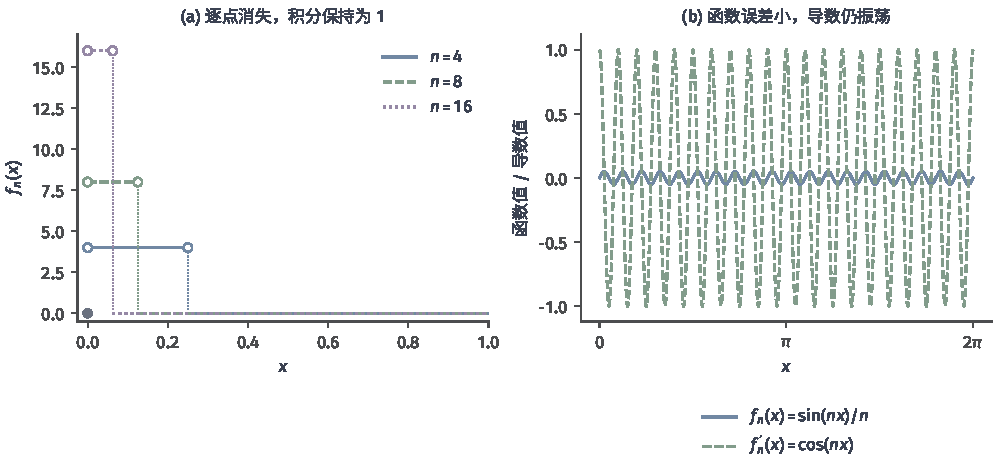
\includegraphics[width=169.0mm]{figures/01-mathematical-preliminaries-upper/01-mathematical-language-combinatorics-analysis-optimization/matplotlib/analysis-convergence-obstacles/figure.pdf}
  \caption{两种交换运算的障碍。左图的尖峰支撑不断收缩，但高度同步增长，每条曲线的积分仍为$1$；开圆点标出不取的上端点，竖虚线仅提示跳跃。右图取$n=20$，$\sin(nx)/n$的函数幅度很小，导数$\cos(nx)$仍有单位幅度。两图均为按给定函数公式构造的教学示例。}
 \label{fig:analysis-convergence-obstacles}
\end{figure*}

表~\ref{tab:analysis-interchange-conditions}汇总极限与勒贝格积分交换的不同条件。积分等式成立的依据来自这些条件，不能仅由点态极限的存在推出。
\begin{table*}[htbp]
 \centering\small
 \begin{tabularx}{\linewidth}{@{}lXX@{}}
 \toprule
 结果 & 核对的条件 & 可得到的结论\\
 \midrule
 有限测度上一致收敛 & 各项可积，且全部输入的误差一致趋零 & 极限可积，积分可交换极限\\
 单调收敛 & 非负可测函数逐点或几乎处处递增 & 极限与积分相等，允许无穷值\\
 Fatou引理 & 非负可测函数列 & 先取下极限再积分，不超过先积分再取下极限的结果\\
 支配收敛 & 几乎处处收敛，且共用一个可积绝对上界 & 积分可交换极限，并有$\int|f_n-f|\,\mathrm dm\to0$\\
 \bottomrule
 \end{tabularx}
 \caption{极限与勒贝格积分之间的交换条件。表中的测度、可测性和统一控制属于结论的假设。}
 \label{tab:analysis-interchange-conditions}
\end{table*}


本小节的三类结论控制的运算不同：保留连续性需要共同的函数值误差，交换微分还要控制导数，交换积分则要检查有限测度、非负单调性或共同可积支配等相应条件。表~\ref{tab:analysis-interchange-conditions}中的条件及前面的反例给出了各自的适用边界。

\subsection{函数项级数的极限}
\label{sec:analysis-function-series-limits}

函数列的极限比较一列已经给定的函数；函数项级数则把不断加入的函数项累计起来。
给定$u_n:X\to\mathbb R$，记部分和$S_N(x)=\sum_{n=1}^Nu_n(x)$，研究$\sum_{n=1}^\infty u_n(x)$就是研究函数列$(S_N)$。
下面先按部分和区分收敛方式，再判断何时收敛，以及求导或积分能否移入无穷求和。

\subsubsection{收敛方式与判别}

部分和把级数化成函数列，前面几种收敛方式都可以沿用，但必须说明它们约束的是部分和，而不是单个函数项$u_n$。
下面逐一给出定义；判据则是把函数列的柯西判据用于部分和。

\paragraph{点态收敛}
固定输入后，函数项级数就是一个数项级数，点态收敛要求每个这样的数项级数都收敛。
\begin{definition}[函数项级数的点态收敛]
\label{def:analysis-series-pointwise-convergence}
设$X\subseteq\mathbb R$，$u_n:X\to\mathbb R$，$S_N=\sum_{n=1}^Nu_n$。若存在$u:X\to\mathbb R$，使部分和$S_N$在$X$上点态收敛到$u$，即对每个$x\in X$都有$\sum_{n=1}^\infty u_n(x)=u(x)$，就称函数项级数$\sum_nu_n$在$X$上点态收敛，$u$称为它的和函数。
\end{definition}
尾部起点可以随$x$改变。特别地，$u_n(x)\to0$只是必要条件，不能代替部分和收敛。

\paragraph{点态收敛的判据}
未知和函数时，比较两个较晚的部分和；它们的差是一段有限尾和，因此点态收敛等价于
\[
 \begin{gathered}
 \forall x\in X,\quad\forall\varepsilon>0,\quad\exists N=N(x,\varepsilon),\\
 m>n\geq N\Longrightarrow
 \left|\sum_{k=n+1}^{m}u_k(x)\right|<\varepsilon.
 \end{gathered}
\]
这是将定理~\ref{thm:analysis-pointwise-cauchy-criterion}用于$S_N$，与对数项级数逐点使用柯西准则完全一致。

\paragraph{一致收敛}
若希望同一个项数同时控制全部输入处的截断误差，就要求部分和一致收敛。
\begin{definition}[函数项级数的一致收敛]
\label{def:analysis-series-uniform-convergence}
设$\sum_nu_n$在$X$上点态收敛到和函数$u$。若部分和$S_N$在$X$上一致收敛到$u$，即
\[
 \sup_{x\in X}\left|u(x)-\sum_{n=1}^Nu_n(x)\right|\longrightarrow0\qquad(N\to\infty),
\]
就称函数项级数在$X$上一致收敛。
\end{definition}
同一个$N$控制全部输入处的剩余和。例如在$[0,1)$上，$\sum_{n=0}^\infty x^n$逐点收敛到$1/(1-x)$，但收敛不一致：若一致收敛，可取$N$使$|u-S_N|<1$在$[0,1)$上成立，有界的部分和$S_N$便迫使和函数$u\leq S_N+1$有界，与$1/(1-x)$无界矛盾。
若每个$u_n$连续，有限部分和也连续，一致收敛便由定理~\ref{thm:analysis-uniform-continuity-limit}保证和函数连续。

\paragraph{一致收敛的判据}
若希望得到一致收敛，就要把尾部起点的选择放在选择输入之前。
由定理~\ref{thm:analysis-uniform-cauchy-criterion}，一致收敛当且仅当
\[
 \begin{gathered}
 \forall\varepsilon>0,\quad\exists N,\quad\forall x\in X,\\
 m>n\geq N\Longrightarrow
 \left|\sum_{k=n+1}^{m}u_k(x)\right|<\varepsilon.
 \end{gathered}
\]
这里不预先指定和函数：实数的完备性先提供各点的极限，共同的尾和界再使收敛一致。

\paragraph{几乎处处收敛}
积分只关心零测集之外的取值，因此也可以只要求部分和在零测集之外收敛。
\begin{definition}[函数项级数的几乎处处收敛]
\label{def:analysis-series-almost-everywhere-convergence}
设$E\in\mathcal L(\mathbb R)$，$u_n:E\to\mathbb R$可测。若存在零测集$N_0\subseteq E$，使对每个$x\in E\setminus N_0$，部分和$S_N(x)$都收敛到有限值$u(x)$，就称$\sum_nu_n$在$E$上几乎处处收敛到$u$。
\end{definition}
可以把和函数在$N_0$上取为零，它仍可测。几乎处处收敛与点态收敛的区别是允许一个固定的零测例外，它并未提供全域共同的误差界。

\paragraph{绝对收敛}
正负项相消可能使部分和收敛，而绝对值级数仍发散；绝对收敛排除了这种相消。
\begin{definition}[函数项级数的绝对收敛]
\label{def:analysis-series-absolute-convergence}
若对每个$x\in X$，数项级数$\sum_n|u_n(x)|$都收敛，就称级数$\sum_nu_n$在$X$上绝对收敛。若$X=E$是可测集，而这一条件只在某个零测集之外成立，就称该级数几乎处处绝对收敛。
\end{definition}
由数项级数的绝对收敛判别，绝对收敛能保证相应位置的级数收敛，却不自动给出一致收敛；后者还需要对全部输入共同适用的尾和控制。例如$\sum_{n\geq0}x^n$在$[0,1)$上每点绝对收敛，却不一致收敛。

\paragraph{Weierstrass判别法}
逐一估计所有输入处的尾和可能很困难。若每一项都能用一个与输入无关的非负数控制，就可以把函数项级数归约为已知的数项级数。
\begin{theorem}[Weierstrass判别法]
\label{thm:analysis-weierstrass-series-test}
设$X$非空，$u_n:X\to\mathbb R$。若存在非负实数$M_n$使
\[
 \forall x\in X,\quad |u_n(x)|\leq M_n,
 \qquad \sum_{n=1}^{\infty}M_n<\infty,
\]
则$\sum_nu_n$在每个$x$处绝对收敛，并在$X$上一致收敛到某个实值函数$u$。
此外，截断误差满足
\[
 \sup_{x\in X}\left|u(x)-\sum_{n=1}^Nu_n(x)\right|
 \leq\sum_{n>N}M_n\longrightarrow0.
\]
\end{theorem}
\begin{proof}
对每个固定$x$，比较判别给出$\sum_n|u_n(x)|\leq\sum_nM_n<\infty$，故和$u(x)$存在。
对任意$m>N$，三角不等式给出$|\sum_{n=N+1}^m u_n(x)|\leq\sum_{n>N}M_n$。
令$m\to\infty$并对$x$取上确界，就得到所述误差界；数项级数的尾和趋零，故收敛一致。
\end{proof}
例如在$[-1,1]$上，$u_n(x)=x^n/2^n$满足$|u_n(x)|\leq2^{-n}$，而$\sum_{n>N}2^{-n}=2^{-N}$。
这个共同的几何尾和控制全部输入处的截断误差；每个函数项连续，所以和函数也连续。
判别法只是充分条件，不能把“没有找到这样的$M_n$”当成不一致收敛的证明。

\subsubsection{逐项求导}

部分和总可以有限次求导，问题在于求导后再取极限，是否得到和函数的导数。
仅有原级数一致收敛还不够；下面把控制施加在导数级数上，并用一个点的函数值确定累计常数。
\begin{theorem}[函数项级数的逐项求导]
\label{thm:analysis-function-series-differentiation}
设$u_n\in C^1([a,b])$。若存在$x_0\in[a,b]$使$\sum_nu_n(x_0)$收敛，且导数级数$\sum_nu_n'$在$[a,b]$上一致收敛，则$\sum_nu_n$在$[a,b]$上一致收敛到某个$u\in C^1([a,b])$，且
\[
 u'(x)=\sum_{n=1}^{\infty}u_n'(x).
\]
\end{theorem}
\begin{proof}
取$S_N=\sum_{n=1}^Nu_n$，则$S_N(x_0)$收敛，$S_N'=\sum_{n=1}^Nu_n'$一致收敛。
将函数列导数的一致收敛结论（定理~\ref{thm:analysis-uniform-derivative-limit}）用于$S_N$，即得原级数一致收敛、和函数连续可微以及导数公式。
\end{proof}
实际验证时，常对导数级数$\sum_nu_n'$使用Weierstrass判别法；要找的是$|u_n'|$的共同上界，而不是$|u_n|$的共同上界。
若函数项只有绝对连续性，也可将定理~\ref{thm:analysis-integral-derivative-limit}用于部分和：单点处的级数收敛，且导数部分和按绝对误差积分趋于某个可积函数$g$时，和函数绝对连续，并有$u'=g$几乎处处。
这里$g$是导数部分和在积分误差意义下的极限，不能额外断言导数级数在每个点都收敛。

\subsubsection{逐项积分}

有限部分和的积分总可以写成有限和，能否再令项数趋于无穷，则取决于对部分和积分的控制。
非负项、绝对积分的总和有限以及有限测度上的一致收敛，给出三种不同的充分条件。以下设$E\in\mathcal L(\mathbb R)$。

\paragraph{非负函数项级数的逐项积分}
非负项使部分和递增，因此可以直接使用单调收敛定理，不要求总积分有限。
\begin{theorem}[非负函数项级数的逐项积分]
\label{thm:analysis-nonnegative-series-integration}
若$u_n:E\to[0,\infty]$可测，则
\[
 \int_E\sum_{n=1}^{\infty}u_n\,\mathrm dm
 =\sum_{n=1}^{\infty}\int_Eu_n\,\mathrm dm,
\]
两边均允许为$+\infty$。
\end{theorem}
\begin{proof}
非负部分和$S_N$递增到$\sum_nu_n$。用单调收敛定理交换极限与积分，再对每个$S_N$用有限加法，即得等式。
\end{proof}

\paragraph{绝对积分总和有限时的逐项积分}
有正负项时，绝对值的累计可以同时控制无穷求和中的抵消及积分误差。
下面的条件既保证和函数可积，也保证部分和按绝对误差积分趋于和函数。
\begin{theorem}[绝对积分可求和的函数项级数]
\label{thm:analysis-absolutely-integrable-series}
若$u_n:E\to\mathbb R$可测且$\sum_n\int_E|u_n|\,\mathrm dm<\infty$，则$\sum_nu_n$几乎处处绝对收敛。
将和函数在绝对值级数发散的零测集上定义为零，所得$u$可积，并有
\[
 \int_E\left|u-\sum_{n=1}^Nu_n\right|\,\mathrm dm
 \leq\sum_{n>N}\int_E|u_n|\,\mathrm dm\longrightarrow0,
\]
从而
\[
 \int_Eu\,\mathrm dm=\sum_{n=1}^{\infty}\int_Eu_n\,\mathrm dm.
\]
\end{theorem}
\begin{proof}
由非负级数的逐项积分，$G=\sum_n|u_n|$满足$\int_EG\,\mathrm dm<\infty$，故$G<\infty$几乎处处。
在零测集$N_0=\{G=\infty\}$之外，级数绝对收敛，且$|u|\leq G$；在$N_0$上取$u=0$后，$u$仍可测且可积。
对几乎每个$x$，$|u(x)-S_N(x)|\leq\sum_{n>N}|u_n(x)|$。
对这一不等式积分，再对右侧的非负尾级数逐项积分，得到所述误差界。
积分之差不超过绝对误差的积分，而有限部分和满足$\int S_N=\sum_{n=1}^N\int u_n$，令$N\to\infty$便得到结论。
\end{proof}

\paragraph{有限测度上一致收敛时的逐项积分}
还有一种充分条件直接约束部分和的共同误差，而不要求绝对积分的总和有限。
若$m(E)<\infty$、各$u_n$可积，且部分和$S_N$一致收敛到$u$，则定理~\ref{thm:analysis-uniform-lebesgue-integral-limit}给出
\[
 \int_Eu\,\mathrm dm
 =\lim_{N\to\infty}\int_ES_N\,\mathrm dm
 =\sum_{n=1}^{\infty}\int_Eu_n\,\mathrm dm.
\]
这里的关键是有限总测度乘一致误差趋零；它与定理~\ref{thm:analysis-absolutely-integrable-series}的绝对可求和条件是两项不同的条件，应分别检查。

\subsection{反常积分}
\label{sec:analysis-improper-integrals}

前面的有限区间计算还留下两个问题：积分范围延伸到无穷远时怎样累计，函数在端点或内部某点附近无界时怎样累计。
这两类问题通常称为\term{反常积分}（improper integral）。下面先分别说明定义与截断方式，再集中判断何时可积。
本小节沿用勒贝格积分的约定：非负函数的积分允许为无穷，有符号函数的有限可积性要求绝对值的积分有限；截断只用来计算已有的积分，不把按指定顺序得到的抵消另算作有限的勒贝格积分。

\subsubsection{无穷区间上反常积分的定义}

先设$f$在每个有限区间$[a,R]$上勒贝格可积，唯一待处理的是无穷远处的尾部。
把积分范围延伸到半轴，就得到这一类反常积分的记号。
\begin{definition}[无穷区间上的反常积分]
\label{def:analysis-improper-infinite-interval}
设$f:[a,\infty)\to\mathbb R$可测，且在每个$[a,R]$上可积。
将$[a,\infty)$上的勒贝格积分记为
\[
 \int_a^\infty f(x)\,\mathrm dx:=\int_{[a,\infty)}f\,\mathrm dm,
\]
称为无穷区间上的反常积分。
若$f\geq0$，该值属于$[0,\infty]$；若$f$有正负值，本节讨论其有限积分时要求$\int_a^\infty|f|<\infty$。
\end{definition}
这个记号可以通过有限范围上的计算求值。非负时由单调收敛定理，有
\[
 \int_a^\infty f(x)\,\mathrm dx
 =\lim_{R\to\infty}\int_a^R f(x)\,\mathrm dx,
\]
允许为无穷；有符号且绝对可积时，以$|f|$为支配函数，对$f\mathbb I_{[a,R]}$使用支配收敛定理，也得到同一有限等式。
严格说，两个收敛定理先沿一列$R_n\uparrow\infty$使用；非负累计关于$R$的单调性，或遗漏范围上绝对积分趋零，再保证任意方式的$R\to\infty$都得到相同结论。

左半轴作相同处理。整个实轴上还需分别处理左右两端：对任意固定的$c\in\mathbb R$，$f$可积当且仅当两侧的绝对值积分都有限，此时
\[
 \int_{\mathbb R}f\,\mathrm dm
 =\int_{(-\infty,c]}f\,\mathrm dm+\int_{(c,\infty)}f\,\mathrm dm.
\]
只知道对称截断$[-R,R]$中的正负抵消稳定，不能代替左右两侧可积，示例~\ref{ex:analysis-sign-function-no-integral}已经说明这一点。

\subsubsection{无界函数反常积分的定义}

范围有限时，函数仍可能在端点附近无界。先避开该端点计算，再检查遗漏的短区间是否保留了不可忽略的累计。
\begin{definition}[无界函数的反常积分]
\label{def:analysis-improper-unbounded-function}
设$f:(a,b]\to\mathbb R$可测，在每个$[c,b]$（$a<c<b$）上可积，并允许在$a$附近无界。
将$(a,b]$上的勒贝格积分记为
\[
 \int_a^bf(x)\,\mathrm dx:=\int_{(a,b]}f\,\mathrm dm,
\]
称为在端点$a$处的反常积分。
若$f\geq0$，该值允许为$+\infty$；若$f$有正负值，本节讨论其有限积分时要求$\int_{(a,b]}|f|\,\mathrm dm<\infty$。
\end{definition}
非负时，$f\mathbb I_{[c,b]}$随$c\downarrow a$逐步增加到$f$；有符号且绝对可积时，这些截断函数由$|f|$支配。
因此分别用单调收敛定理或支配收敛定理得到
\[
 \int_{(a,b]}f\,\mathrm dm=\lim_{c\downarrow a}\int_c^bf(x)\,\mathrm dx.
\]
若无界位置在右端点，就从左侧截断；若在内部点$s$，则把$(a,s)$与$(s,b)$分开累计，有符号的有限积分要求两侧均绝对可积。
在单点上赋予有限值不改变勒贝格积分，因而决定可积性的是该点附近的累计，而不是该点取了什么值。


图~\ref{fig:analysis-process-improper-two-truncations}对照两种截断：向外扩大累计范围，或从奇点附近逐渐补回遗漏的范围。
\begin{figure*}[!htbp]
 \centering
 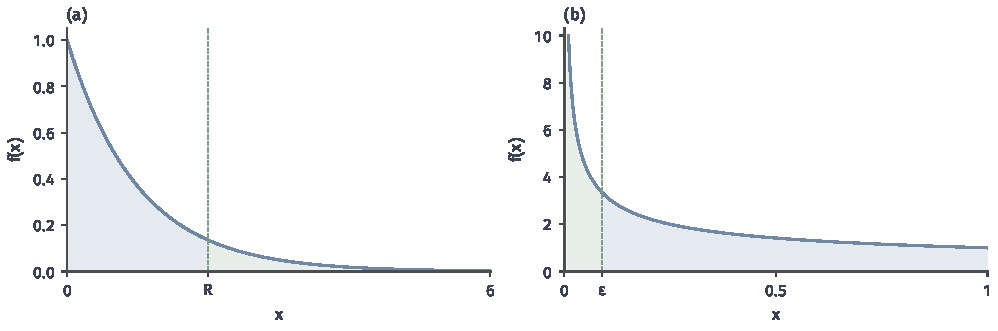
\includegraphics[width=169.0mm]{figures/01-mathematical-preliminaries-upper/01-mathematical-language-combinatorics-analysis-optimization/matplotlib/chapter3-concept-processes/improper-two-truncations.pdf}
 \caption{(a) $e^{-x}$在$[0,\infty)$上，以$R=2$截断，蓝区已计入，绿区属于遗漏尾部，其完整积分为$e^{-2}$；图只显示到$x=6$。(b) $x^{-1/2}$在$(0,1]$上，以$\varepsilon=0.09$截断，完整遗漏积分为$2\sqrt\varepsilon$。右图曲线只绘$x\geq0.01$，未画出的更近零点部分仍属积分范围。}
 \label{fig:analysis-process-improper-two-truncations}
\end{figure*}

\subsubsection{反常积分的可积性}

两种截断都可以写为递增的可测范围$E_n\uparrow E$：范围不断向外延伸，或者从被避开的奇异位置逐步收回遗漏的部分。
因此可以用同一个判据回答可积性问题，随后再用截断积分或原函数计算具体数值。

\paragraph{简单函数与截断函数的积分收敛}
函数列的收敛定理补上了前面几种逼近中积分极限的依据。对非负可测$f$，规范简单逼近$s_n$逐点递增到$f$，单调收敛定理给出$\int s_n\uparrow\int f$。

若$f$绝对可积，按高度截断的$f_n=\max\{-n,\min\{f,n\}\}$满足$f_n\to f$且$|f_n|\leq|f|$，支配收敛定理给出$\int|f_n-f|\to0$。
在实轴上按范围截断的$f\mathbb I_{[-n,n]}$同样被$|f|$支配。这与前面的无穷范围截断相对应，说明有限范围上的计算可以逼近全域上的积分。

\paragraph{非负函数的可积性}
非负累计随截断范围扩大而增加，积分有限的关键在于这些累计能否被同一个有限常数控制。
\begin{theorem}[非负截断累计的有界判据]
\label{thm:analysis-improper-nonnegative-criterion}
设$E\in\mathcal L(\mathbb R)$，$f:E\to[0,\infty]$可测，$E_n$为递增可测集且$\bigcup_nE_n=E$。则
\[
 \int_Ef\,\mathrm dm<\infty
 \quad\Longleftrightarrow\quad
 \sup_n\int_{E_n}f\,\mathrm dm<\infty,
\]
并有$\int_Ef\,\mathrm dm=\lim_n\int_{E_n}f\,\mathrm dm$。
\end{theorem}
\begin{proof}
因为$0\leq f\mathbb I_{E_n}\uparrow f$，单调收敛定理使全域积分等于截断积分序列的极限，也就是其上确界。
因此全域积分有限恰好等价于这些截断积分有共同的有限上界。
\end{proof}
在无穷半轴上可取$E_n=[a,a+n]$，在奇异端点$a$附近可取$E_n=[a+(b-a)/(n+1),b]$。
只知道每一个截断积分分别有限还不够，还要检验它们是否有共同的上界。

由积分的单调性还得到比较原则：若$0\leq f\leq g$几乎处处且$\int g<\infty$，则$\int f<\infty$；反之，若$0\leq g\leq f$且$\int g=\infty$，则$\int f=\infty$。
最基本的比较对象是幂函数，它们的截断积分可以用原函数算出。
\begin{example}[用截断计算幂函数的反常积分]
\label{ex:analysis-power-integral-truncations}
在$(0,1]$上取$E_n=[1/n,1]$。由原函数$2\sqrt x$与$\log x$，
\[
 \int_{1/n}^1x^{-1/2}\,\mathrm dx=2(1-n^{-1/2})\longrightarrow2,
 \qquad
 \int_{1/n}^1x^{-1}\,\mathrm dx=\log n\longrightarrow+\infty.
\]
由定理~\ref{thm:analysis-improper-nonnegative-criterion}，$\int_0^1x^{-1/2}\,\mathrm dx=2$，而$\int_0^1x^{-1}\,\mathrm dx=+\infty$。
在$[1,\infty)$上取$E_n=[1,n]$，同理有$\int_1^nx^{-2}\,\mathrm dx=1-1/n\to1$与$\int_1^nx^{-1}\,\mathrm dx=\log n\to+\infty$，所以$\int_1^\infty x^{-2}\,\mathrm dx=1$，而$\int_1^\infty x^{-1}\,\mathrm dx=+\infty$。
\end{example}
这几项计算始终使用同一个勒贝格积分定义，极限等式由单调收敛定理保证。

同一个幂函数在奇点附近与在无穷远处的可积条件恰好相反。不求原函数，也可以用二进分段与几何级数判断$x^{-p}$在两端的可积性。
\begin{example}[幂函数$x^{-p}$的可积阈值]
\label{ex:analysis-power-integrability-thresholds}
先看无穷远处。对$p>0$，$x^{-p}$在$[2^k,2^{k+1}]$上递减，把它在该段的最小值和最大值分别乘以区间长度$2^k$，得到
\[
 2^{-p}2^{k(1-p)}\leq\int_{2^k}^{2^{k+1}}x^{-p}\,\mathrm dx\leq2^{k(1-p)}.
\]
由区域可加性，$\int_1^\infty x^{-p}\,\mathrm dx$等于这些分段积分对$k\geq0$之和。$p>1$时上界$2^{k(1-p)}$是公比小于一的几何数列，部分和有共同上界$1/(1-2^{1-p})$，所以积分有限；$0<p\leq1$时每段至少贡献$2^{-p}$，累计发散。$p\leq0$时在$x\geq1$上$x^{-p}\geq1$，也发散。

再看零点附近。对$p>0$，比较$[2^{-(k+1)},2^{-k}]$上的最小值与最大值，得到该段积分介于$2^{k(p-1)}/2$与$2^{p-1}2^{k(p-1)}$之间；这组几何数列的公比为$2^{p-1}$，所以对$k\geq0$求和恰在$p<1$时有限。$p\leq0$时$x^{-p}$在$(0,1]$上有界（可连续延拓到$0$），本来就可积。

于是$\int_0^1x^{-p}\,\mathrm dx$恰在$p<1$时有限，$\int_1^\infty x^{-p}\,\mathrm dx$恰在$p>1$时有限。
\end{example}
分段常数比较与几何级数给出可积性的阈值，原函数则能进一步算出有限截断的具体数值；$p=1/2$与$p=2$的结果与示例~\ref{ex:analysis-power-integral-truncations}一致。

\paragraph{有符号函数的可积性}
正负值抵消可能使截断积分保持有限，但可积性要求正、负两部分各自具有有限的累计。
因此应把定理~\ref{thm:analysis-improper-nonnegative-criterion}的非负判据用于$|f|$，而不是用于有正负抵消的$f$。
\begin{theorem}[绝对截断累计的可积性判据]
\label{thm:analysis-improper-signed-criterion}
设$E\in\mathcal L(\mathbb R)$，$f:E\to\mathbb R$可测，$E_n\uparrow E$为可测范围，则$f$可积当且仅当
\[
 \sup_n\int_{E_n}|f|\,\mathrm dm<\infty.
\]
可积时，每个截断积分有限，且
\[
 \left|\int_Ef\,\mathrm dm-\int_{E_n}f\,\mathrm dm\right|
 \leq\int_{E\setminus E_n}|f|\,\mathrm dm\longrightarrow0.
\]
所以任意这样的递增穷尽都得到同一个积分值。
\end{theorem}
\begin{proof}
将非负截断判据用于$|f|$，即得充要条件。可积时，区域可加性把积分之差写成遗漏范围上的积分，再用绝对值界得到误差不等式。
函数$|f|\mathbb I_{E\setminus E_n}$逐点趋零且由可积的$|f|$支配，故其积分趋零。
\end{proof}
绝对值尾部既用于判断可积性，也控制有限计算的误差。

例如$p>1$时，把$x^{-p}$在$[1,\infty)$上截断到$[1,R]$（$R>1$），由区域可加性，截断误差恰为尾部积分$\int_R^\infty x^{-p}\,\mathrm dx$，它正是定理~\ref{thm:analysis-improper-signed-criterion}中误差界的右侧。按$[2^jR,2^{j+1}R]$分段比较，得到
\[
 \int_R^\infty x^{-p}\,\mathrm dx
 \leq R^{1-p}\sum_{j=0}^\infty2^{j(1-p)}
 =\frac{R^{1-p}}{1-2^{1-p}}\longrightarrow0.
\]
非负积分的可数区域可加性保证分段求和合法，几何尾和给出显式的误差界。

函数列极限部分留下了一个问题：可积的支配函数本身可以无界。有了$x^{-1/2}$的可积性，就能核对这样的例子。
\begin{example}[无界的可积支配函数]
\label{ex:analysis-unbounded-dominating}
在$(0,1)$上令$f_n(x)=x^n/\sqrt x=x^{n-1/2}$。对每个$x\in(0,1)$，$f_n(x)\to0$；并且$0\leq f_n\leq x^{-1/2}$。
支配函数$x^{-1/2}$在$0$附近无界，但由示例~\ref{ex:analysis-power-integral-truncations}，$\int_0^1x^{-1/2}\,\mathrm dx=2<\infty$，所以支配收敛定理保证$\int_0^1f_n\,\mathrm dx\to0$。
直接计算也得到同一结论：截断后用原函数，$\int_0^1x^{n-1/2}\,\mathrm dx=(n+1/2)^{-1}\to0$。
\end{example}
支配条件要求共同上界的积分有限，不要求上界本身有界。

积分有限要求正负两部分都有限，不能从某一列截断积分有有限极限直接推出。
下面两个例子只说明这种推断为什么失效，不把截断相消作为新的积分规则。先看连续函数在无穷区间上的截断相消。
\begin{example}[$\sin x/x$的截断极限存在但不绝对可积]
\label{ex:analysis-sine-over-x}
在$[1,\infty)$上，取$u(x)=1/x$、$v'(x)=\sin x$作分部积分，得到
\[
 \int_1^R\frac{\sin x}{x}\,\mathrm dx
 =\cos1-\frac{\cos R}{R}-\int_1^R\frac{\cos x}{x^2}\,\mathrm dx.
\]
$R\to\infty$时端点项$\cos R/R\to0$；最后一项的被积函数满足$|\cos x/x^2|\leq x^{-2}$，绝对可积，由定理~\ref{thm:analysis-improper-signed-criterion}收敛到有限值。所以截断积分存在有限极限。
但在每个$[k\pi+\pi/6,k\pi+5\pi/6]$（$k\geq1$）上，$|\sin x|\geq1/2$且$x\leq(k+1)\pi$，区间长为$2\pi/3$，故该段的绝对积分至少为$1/(3(k+1))$。
这些区间两两不交，调和级数发散，所以$\int_1^\infty|\sin x|/x\,\mathrm dx=+\infty$。
\end{example}
这个有限的截断极限依赖正负抵消，不是本章所用的有限勒贝格积分。

奇点两侧的抵消也有同样的问题。
\begin{example}[$1/x$的柯西主值]
\label{ex:analysis-cauchy-principal-value}
在$(-1,1)$上取$f(x)=1/x$，原点处赋值为零。
由示例~\ref{ex:analysis-power-integral-truncations}，$\int_0^1x^{-1}\,\mathrm dx=+\infty$，对称地负部在$(-1,0)$上的积分也为无穷，所以$f$没有有符号勒贝格积分。
但对称截断满足
\[
 \lim_{\varepsilon\downarrow0}\left(
 \int_{-1}^{-\varepsilon}\frac{\mathrm dx}{x}
 +\int_{\varepsilon}^{1}\frac{\mathrm dx}{x}\right)
 =\lim_{\varepsilon\downarrow0}\bigl(\log\varepsilon-\log\varepsilon\bigr)=0.
\]
若改用非对称截断$\int_{-1}^{-\varepsilon}+\int_{2\varepsilon}^1$，两项之和恒为$\log\varepsilon-\log(2\varepsilon)=-\log2$，极限变为$-\log2$。
\end{example}
对称相消的极限称为柯西主值。它的数值依赖截断方式，没有使$\int|f|$变为有限，也没有定义出本章采用的勒贝格积分。
后续计算仍只使用非负函数的积分（允许为无穷）或绝对可积函数的有限积分。

\FloatBarrier


\FloatBarrier
\section{本章小结}
\label{sec:analysis-summary}
\label{sec:measurable-summary}

连续性把输入趋近与输出趋近联系起来；一致连续、Lipschitz连续和绝对连续分别加强不同的控制要求。
一元可微性把函数增量写成斜率乘输入增量，中值定理、Taylor余项和导数上界说明局部信息怎样控制有限变化。
测度规定可测集合的大小，同一种距离并不唯一决定集合权重。
有限区间逼近形成Jordan测量，可数覆盖形成外测度，可测分割条件使其在允许的集合族上恢复可数可加等式。
黎曼积分从区间分割出发，勒贝格积分按可测集合及简单函数累计；有界区间上的黎曼可积函数也勒贝格可积，积分值相同，反向包含不成立。
不定积分由原函数定义，变上限积分由累计构造定义，二者的联系需要微积分基本定理。
连续被积函数的累计可逐点求导，勒贝格可积函数一般只保证几乎处处恢复；绝对连续恰好保证函数可以通过可积导数恢复。
连续函数的一致极限连续，微分交换还需控制导数，积分交换还需有限测度、单调性或共同可积支配等条件。
无穷范围与奇点仍按同一积分定义累计，截断方式和绝对值尾部决定计算能否恢复全域积分，指定相消极限不能代替可积性。

\chapter{多元函数微积分}
\label{chap:multivariate-calculus}
\label{chap:multivariable-functions}

当输入由一个实数变为多个坐标时，逐坐标观察是否足以描述整体变化？累计范围由区间变为区域、路径或曲面时，又应使用怎样的权重和方向？
本章使用第~\ref{chap:linear-algebra-and-matrix-analysis}章的向量与线性映射、
第~\ref{chap:function-limits}章的距离与极限，以及第~\ref{chap:univariate-calculus}章的一元微分和勒贝格积分。
先研究联合趋近、全微分与共同的线性近似，再分别建立区域、路径和曲面上的积分。
最后用Green、Gauss和Stokes公式联系内部导数的累计与边界贡献，逐一核对正则性、可积性和定向条件。

\par\Needspace{14\baselineskip}
\section{多元函数的微分}
\label{sec:analysis-multivariable-differentiation}
\label{sec:multivariable-differentiation}

一元微分用一个斜率描述输入微调后的输出变化。对$f(x,y)=x^2+xy+y^2$，输入是二维点而输出仍是一个实数；若同一输入同时产生多个实数，才得到向量值函数。
下面先完整研究多元标量函数，再将线性近似推广到向量输出；矩阵自变量及局部方程的求解各自另作讨论。
这样，梯度始终对应标量输出，Jacobian矩阵始终记录多个输出分量的变化，二者的形状与作用不会混用。
向量、矩阵、迹与行列式沿用第~\ref{chap:sets-functions-and-proofs}章；极限与距离沿用第~\ref{chap:function-limits}章，连续、微分与勒贝格积分沿用第~\ref{chap:univariate-calculus}章的结论。
偏导数与局部线性近似可参考\scite{math-openstax-calculus3}，严格的多元微分论证可参考\scite{math-lebl2026analysis2}。

\subsection{多元标量函数的极限和连续性}
\label{sec:multivariable-limits-continuity}

本小节始终研究$f:D\subseteq\mathbb R^d\to\mathbb R$。多个输入坐标必须共同趋近一个点，输出误差则仍用实数绝对值度量。

\subsubsection{多元标量函数的定义}

固定一个坐标得到一元切片，恢复全部坐标后才是原来的多元函数。先明确输入与输出，才能区分“沿某个切片趋近”和“整个定义域中的趋近”。
\begin{definition}[多元标量函数]
\label{def:multivariable-scalar-function}
设$d$为正整数、$D\subseteq\mathbb R^d$。映射$f:D\to\mathbb R$称为多元标量函数；它把整个输入点$\bm x=(x_1,\ldots,x_d)^\top$映为一个实数$f(\bm x)$。
\end{definition}
例如$f(x,y)=x^2+xy+y^2$在$(1,2)$处取值$7$；固定$y=2$后得到的一元切片是$x\mapsto x^2+2x+4$，它只反映原函数在一条直线上的取值。

\subsubsection{极限的定义与判别}

在实轴上可以从左右两侧趋近，在平面中还可以沿直线、抛物线等路径趋近。
极限必须同时控制所有允许的输入，不能按路径分别选择互不兼容的误差范围。
\paragraph{极限的定义}
\label{sec:multivariable-joint-limits}

设$\bm D\subseteq\mathbb R^d$，$f:\bm D\to\mathbb R$，
$\bm a$是$\bm D$的聚点，即任意小的球内都有不同于$\bm a$的定义域点。
用欧氏距离$\lVert\bm x-\bm a\rVert_2$同时控制各坐标的偏移，便能把一元极限的邻域条件推广过来。
\begin{definition}[多元函数的极限]
\label{def:multivariable-limit}
若对每个$\varepsilon>0$，都存在$\delta>0$，使得
\[
 \bm x\in\bm D,\quad 0<\lVert\bm x-\bm a\rVert_2<\delta
 \quad\Longrightarrow\quad |f(\bm x)-L|<\varepsilon,
\]
则称$f$在$\bm x\to\bm a$时的极限为$L$，记为$\lim_{\bm x\to\bm a}f(\bm x)=L$。
\end{definition}
这里的同一个$\delta$必须控制球内全部允许输入。各坐标可以按不同速度趋近，
也可以让行进方向随位置改变。

\paragraph{序列判据与路径检验}
与一元情形一样，极限存在等价于：任意满足$\bm x_n\in\bm D\setminus\{\bm a\}$、
$\bm x_n\to\bm a$的序列都有$f(\bm x_n)\to L$。
这与一般度量空间中的连续性序列判据结构相同，这里是它在欧氏输入、实数输出下的直接应用，所需的输入与输出距离都已指定。
所以找到两条输出极限不同的路径足以否定极限，但验证有限条路径不能证明极限存在。

\begin{example}[坐标切片与所有直线仍会遗漏路径]
\label{ex:multivariable-path-limits}
令$f(0,0)=0$，非原点处令$f(x,y)=xy/(x^2+y^2)$。
沿两条坐标轴，函数都为$0$；沿$y=x$，函数恒为$1/2$，故原点处没有联合极限。
这个函数分别固定一个坐标后，在另一坐标上连续，但它在原点不联合连续。

即使验证所有过原点的直线，仍不足够。令$g(0,0)=0$，并在非原点处令
\[
 g(x,y)=\frac{x^2y}{x^4+y^2}.
\]
沿$y=kx$，当$k\neq0$时$g(x,kx)=kx/(x^2+k^2)\to0$；
当$k=0$或沿竖直轴时，函数为$0$。
可是沿抛物线$y=x^2$，$g(x,x^2)=1/2$。每条固定直线上的控制不能同时控制弯曲的趋近方式。
\end{example}


图~\ref{fig:analysis-process-joint-limit-paths}把直线路径和弯曲路径放到同一函数上，显示只检查直线可能遗漏的趋近方式。
\begin{figure*}[!htbp]
 \centering
 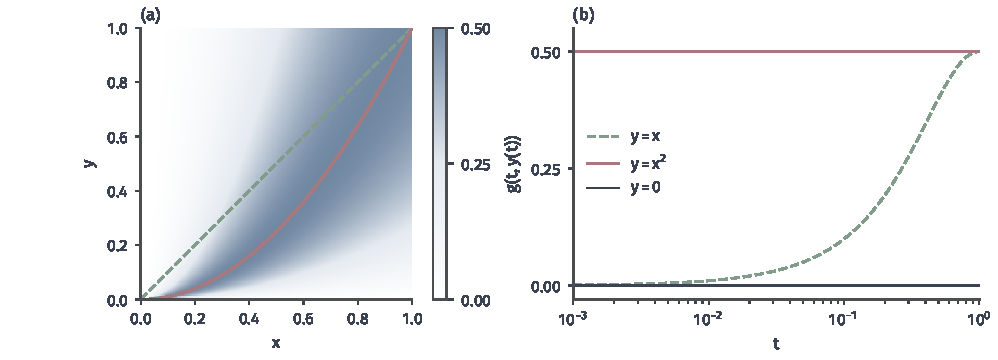
\includegraphics[width=169.0mm]{figures/01-mathematical-preliminaries-upper/01-mathematical-language-combinatorics-analysis-optimization/matplotlib/chapter3-concept-processes/joint-limit-paths.pdf}
 \caption{取前例$g(x,y)=x^2y/(x^4+y^2)$，原点另置零。(a) 第一象限的函数值及三条路径，色阶固定为$0$至$1/2$。(b) 沿$y=0$、$y=x$分别趋零，沿$y=x^2$恒为$1/2$；横轴为正参数$t$的对数刻度，向左趋近原点。不同路径极限足以否定联合极限，有限条路径不能反向证明存在。}
 \label{fig:analysis-process-joint-limit-paths}
\end{figure*}

\paragraph{累次极限与联合极限}
累次极限还会改变问题的量词。先令$y\to0$、再令$x\to0$，考察的是
$\lim_{x\to0}\lim_{y\to0}f(x,y)$，没有要求两个坐标同时趋近。
对上例的$f$，两个次序的累次极限都为$0$，联合极限却不存在。
又如$h(x,y)=x^2/(x^2+y^2)$在非原点定义，则
\[
 \lim_{x\to0}\lim_{y\to0}h(x,y)=1,
 \qquad
 \lim_{y\to0}\lim_{x\to0}h(x,y)=0.
\]
所以累次极限相等不是联合极限存在的充分条件；改变次序也可能改变累次极限。
如果联合极限存在，并且相关内层极限在去心邻域内存在，相应累次极限才必须等于联合极限。

\paragraph{统一误差估计}
要证明联合极限，可以寻找只依赖距离的统一上界。
例如$|xy|\leq(x^2+y^2)/2$，所以
\[
 \left|\frac{x^2y}{x^2+y^2}\right|
 \leq \frac{|x|}{2}
 \leq\frac12\sqrt{x^2+y^2}\longrightarrow0.
\]
这个估计同时覆盖全部路径，因此给出原点极限为$0$。极坐标也可用于估计，
但写成$(x,y)=(r\cos\theta,r\sin\theta)$后，仍需控制所有角度，不能只固定$\theta$再令$r\to0$。

\subsubsection{连续性的定义与运算}
\label{sec:multivariable-continuity}

连续性要求联合趋近时的输出恰好趋于基点值，形式与前面度量下的连续性相同。
这里先对全部输入作共同控制，再讨论运算后能否保留这种控制。
\begin{definition}[多元标量函数的连续性]
\label{def:multivariable-scalar-continuity}
设$f:D\subseteq\mathbb R^d\to\mathbb R$、$\bm a\in D$。若对每个$\varepsilon>0$都存在$\delta>0$，使
\[
 \bm x\in D,\quad\lVert\bm x-\bm a\rVert_2<\delta
 \Longrightarrow |f(\bm x)-f(\bm a)|<\varepsilon,
\]
则称$f$在$\bm a$处连续；在$D$上每点连续时称$f$为连续函数。
\end{definition}
聚点处这等价于联合极限等于$f(\bm a)$，孤立点处则自动成立。固定其他输入坐标后的一元切片连续只是必要条件，例~\ref{ex:multivariable-path-limits}说明它不足以保证联合连续。

\paragraph{和的连续性}
若$f,g$在$\bm a$处连续，则$f+g$也连续，因为和的输出误差不超过两个原误差之和。

\paragraph{差的连续性}
在相同条件下$f-g$连续：差的输出误差同样不超过两个原误差之和。

\paragraph{数乘的连续性}
若$f$在$\bm a$处连续，$c$为固定实数，则$cf$连续。$c\neq0$时将$f$的误差控制在$\varepsilon/|c|$以内即可；$c=0$时结论直接成立。

\paragraph{积的连续性}
若$f,g$在$\bm a$处连续，则$fg$连续。这由两个实数输出的积的极限法则得到。

\paragraph{商的连续性}
若$f,g$在$\bm a$处连续且$g(\bm a)\neq0$，则$g$在基点附近远离零，商的极限法则保证$f/g$连续。分母非零的条件不能省略。
多元多项式由连续坐标函数的有限运算得到，因此连续；分母非零处的有理函数同样连续。

\paragraph{标量复合函数}
若$f:D\to\mathbb R$在$\bm a$处连续，一元函数$\psi$在$f(\bm a)$处连续，且$f$的相邻输出在$\psi$的定义域内，则$\psi\circ f$连续。
先用$\psi$确定中间实数的允许误差，再由$f$控制输入点的欧氏距离，即得到复合函数的误差条件。

\subsubsection{一致连续性与闭有界集上的性质}

一致连续要求同一个输入误差尺度控制全部基点；有界性与最值存在则约束整个定义域上的函数值。
下面用有限维闭有界集内的收敛子列，分别说明这两类整体结论。

\paragraph{有限维闭有界集的收敛子列}
实数列的Bolzano--Weierstrass定理可以逐个坐标使用，得到多维输入所需的子列性质。
这里有界性负责产生收敛子列，闭性则进一步保留极限点。
\begin{theorem}[有限维有界序列的收敛子列]
\label{thm:multivariable-bolzano-weierstrass}
若$(\bm x_n)$是$\mathbb R^d$中的有界序列，则存在严格递增的正整数序列$(n_k)$及$\bm a\in\mathbb R^d$，使$\bm x_{n_k}\to\bm a$。
若所有$\bm x_n$属于闭集$K$，则$\bm a\in K$。
\end{theorem}
\begin{proof}
先用实数列定理选出第一坐标收敛的子列，再从这个子列中选出第二坐标收敛的子列，重复有限次后，全部坐标都收敛。
设各坐标极限组成$\bm a$，由$\lVert\bm x-\bm a\rVert_2\leq\sqrt d\max_j|x_j-a_j|$可知所得子列在欧氏距离下收敛。
若它属于闭集$K$，闭集包含其收敛序列的极限，故$\bm a\in K$。
\end{proof}
有限维闭有界集因此具有前面刚证明的子列性质，下面直接用它证明函数的整体性质；一般度量空间中紧致与序列紧致的等价在第~\ref{chap:metric-spaces}章讨论。

\paragraph{一致连续性}
把连续定义中的$\delta$放在选择基点之前，就得到一致连续的要求。
具体地，对每个$\varepsilon>0$存在$\delta>0$，使所有$\bm x,\bm y\in D$满足$\lVert\bm x-\bm y\rVert_2<\delta$时都有$|f(\bm x)-f(\bm y)|<\varepsilon$。
闭有界集上的逐点连续足以给出这样的共同尺度。
\begin{theorem}[闭有界集上的一致连续性]
\label{thm:multivariable-uniform-continuity}
设$K\subseteq\mathbb R^d$非空、闭且有界，$f:K\to\mathbb R$连续，则$f$在$K$上一致连续。
\end{theorem}
\begin{proof}
定理~\ref{thm:analysis-uniform-continuity}的证明只用到定义域中任意点列都有域内收敛子列，以及连续性。
上一定理已为$K$建立这项子列性质；将输入距离改为欧氏范数，原证明便适用，无需重新构造反例点列。
\end{proof}
存在有限$L$使$|f(\bm x)-f(\bm y)|\leq L\lVert\bm x-\bm y\rVert_2$时，也直接得到一致连续；这是多元标量函数的Lipschitz条件。

\paragraph{有界性与极值达到}
要保证上、下确界由定义域内的点取得，还需要防止取值趋近确界的输入序列逃出定义域。
闭有界集的子列性质正好保留这种极限点。
\begin{theorem}[闭有界集上的极值定理]
\label{thm:multivariable-extreme-value}
设$K\subseteq\mathbb R^d$非空、闭且有界，$f:K\to\mathbb R$连续，则$f$有界，且存在$\bm x_{\min},\bm x_{\max}\in K$满足
\[
 f(\bm x_{\min})\leq f(\bm x)\leq f(\bm x_{\max})\qquad(\bm x\in K).
\]
\end{theorem}
\begin{proof}
定理~\ref{thm:analysis-extreme-value}已证明，定义域内的收敛子列性质与连续性共同保证有界及最值达到。
这里的$K$由定理~\ref{thm:multivariable-bolzano-weierstrass}满足同一子列条件，所以该证明适用，输出仍为实数。
\end{proof}
这些条件是充分保证。整个平面上的$f(x,y)=x^2+y^2$沿$y=0$退化为前面的实轴平方函数反例，所以连续却不一致连续。
在开单位圆盘上，同一函数的上确界为$1$却没有最大点，说明不能直接删去闭性。

\subsection{偏导数和梯度}

下面仍只研究实值函数$f:U\subseteq\mathbb R^d\to\mathbb R$，其中$U$为开集。先计算各坐标切片的变化率，再把这些标量排列为梯度；沿一般方向的变化率也在这里定义。

\subsubsection{偏导数}

开集保证基点附近足够小的双侧坐标扰动仍在定义域内。固定其他坐标后，就可以直接使用一元导数。
\begin{definition}[偏导数]
\label{def:multivariable-partial-derivative}
设$\bm a\in U$，令$\bm e_j$是第$j$个坐标为$1$、其余为$0$的向量。若双侧极限
\[
 \partial_jf(\bm a)=\frac{\partial f}{\partial x_j}(\bm a)
 =\lim_{t\to0}\frac{f(\bm a+t\bm e_j)-f(\bm a)}t
\]
存在且有限，就称它为$f$在$\bm a$处关于$x_j$的\term{偏导数}（partial derivative）。
\end{definition}
它表示只改变第$j$个坐标、其余坐标固定时的变化率。符号$\partial$提醒我们：这里求的是多元函数的一个坐标切片的导数。

例如对$f(x,y)=x^2+xy+y^2$，固定$y$求导得到$f_x=2x+y$；固定$x$得到$f_y=x+2y$。
在$(1,2)$处，两者为$4,5$。具体地，
\[
 \frac{f(1+t,2)-f(1,2)}t=4+t\longrightarrow4.
\]
这里$f_x(1,2)=4$并不意味着同时改变$x,y$时都以斜率$4$变化。每一个偏导数只说明自己的坐标切片。

\subsubsection{梯度}

各偏导数采用相同的基点，但分别对应不同输入坐标。将这些变化率按坐标顺序排列，就能用一个向量记录所有坐标切片的信息。
\begin{definition}[梯度]
\label{def:multivariable-gradient}
若$f:U\to\mathbb R$在$\bm a$处的各一阶偏导数都存在，称列向量
\[
 \nabla f(\bm a)=\bigl(\partial_1f(\bm a),\ldots,\partial_df(\bm a)\bigr)^\top
\]
为$f$在$\bm a$处的\term{梯度}（gradient）。
\end{definition}
对$f(x,y)=x^2+xy+y^2$，有$\nabla f(x,y)=(2x+y,x+2y)^\top$，所以$\nabla f(1,2)=(4,5)^\top$。
梯度的存在只说明各偏导数存在，尚未保证它能预测所有坐标同时改变时的函数增量；这要由后面的可微性判断。

\subsubsection{方向导数}

沿坐标轴求导只是方向变化的一部分。若让多个坐标按一个固定向量共同移动，就得到另一条一元切片。
\begin{definition}[方向导数]
\label{def:multivariable-directional-derivative}
给定向量$\bm v\in\mathbb R^d$，若双侧极限
\[
 D_{\bm v}f(\bm a)
 =\lim_{t\to0}\frac{f(\bm a+t\bm v)-f(\bm a)}t
\]
存在且有限，就称它为沿$\bm v$的\term{方向导数}（directional derivative）。
\end{definition}
本书允许$\bm v$不是单位向量，导数按参数$t$的变化计量；若要表示每单位路程的变化率，应取$\lVert\bm v\rVert_2=1$。
取$\bm v=\bm e_j$便回到偏导数。双侧极限与只令$t\downarrow0$的单侧方向导数要分别判断。

仍取上述$f$，从$(1,2)$沿$\bm v=(1,1)^\top$移动，有
\[
 f(1+t,2+t)=7+9t+3t^2,
 \qquad D_{(1,1)}f(1,2)=9.
\]
改用同向单位向量$\bm u=(1,1)^\top/\sqrt2$，变化率为$9/\sqrt2$。
两者描述同一条直线，但参数速度不同，不能忽略归一化约定。

\subsection{多元标量函数的可微性}
\label{sec:multivariable-total-differentiation}

偏导数和方向导数分别检查固定的坐标轴或直线。若要同时控制任意小扰动，包括方向不断改变的扰动，就需要一个共同的线性近似。

\subsubsection{微分的定义}

预测增量应与扰动的叠加和数乘相容，因此使用线性映射$A:\mathbb R^d\to\mathbb R$。
例如$A(\bm h)=\bm c^\top\bm h$把每个坐标的扰动乘以固定系数再相加；可微性还要求遗漏的误差比扰动长度更小。
\begin{definition}[多元标量函数的可微性与全微分]
\label{def:multivariable-total-differential}
设$U\subseteq\mathbb R^d$开，$f:U\to\mathbb R$，$\bm a\in U$。
若存在一个线性映射$A:\mathbb R^d\to\mathbb R$，使
\begin{equation}
 f(\bm a+\bm h)=f(\bm a)+A(\bm h)+o(\lVert\bm h\rVert_2),
 \qquad\bm h\to\bm0,
\label{eq:analysis-total-differentiability}
\end{equation}
则称$f$在$\bm a$处\term{可微}（differentiable）。线性映射$A$称为该点的\term{全微分}（total differential），记为$\mathrm df_{\bm a}$。
\end{definition}
余项条件是$|f(\bm a+\bm h)-f(\bm a)-A(\bm h)|/\lVert\bm h\rVert_2\to0$。
它要求一个$A$适用于全部趋零扰动，并非先固定一个方向再允许误差控制随方向改变。

\subsubsection{可微性的要求与判别}
\label{sec:analysis-differentiability-relations}

固定开集$U\subseteq\mathbb R^d$、标量函数$f:U\to\mathbb R$与基点$\bm a\in U$。
下面先说明统一线性近似必然满足哪些要求，再给出可核查的充分判别，最后结合蕴含关系与反例，区分偏导数存在、全部双侧方向导数存在、可微和连续可微。

\paragraph{可微的必要条件}
若同一个线性近似有效，它在线性切片上必须与一元导数相同，函数增量本身也必须趋零。
这就把全微分与前面定义的偏导数、梯度及方向导数联系起来。
\begin{theorem}[可微性与梯度、方向导数]
\label{thm:multivariable-differentiable-necessary}
若$f:U\to\mathbb R$在$\bm a$处可微，则$f$在该点连续，各偏导数存在，并且
\[
 \mathrm df_{\bm a}(\bm h)=\nabla f(\bm a)^\top\bm h,
 \qquad D_{\bm v}f(\bm a)=\nabla f(\bm a)^\top\bm v
 \quad(\bm v\in\mathbb R^d).
\]
\end{theorem}
\begin{proof}
线性性给出$A(\bm h)=\sum_jh_jA(\bm e_j)$。由有限和的Cauchy--Schwarz不等式，
\[
 |A(\bm h)|\leq\left(\sum_j|A(\bm e_j)|^2\right)^{1/2}\lVert\bm h\rVert_2.
\]
因此线性项与余项都随$\bm h\to0$而趋零，得到$f$连续。
分别取$\bm h=t\bm e_j$并除以$t$，可知$\partial_jf(\bm a)=A(\bm e_j)$；线性性给出$A(\bm h)=\sum_j\partial_jf(\bm a)h_j$。
再对固定$\bm v$取$\bm h=t\bm v$，余项除以$t$仍趋零，就得到方向导数公式；$\bm v=\bm0$时差商恒为零。
\end{proof}
\begin{example}[二元二次函数的全微分]
\label{ex:multivariable-quadratic-differential}
对二次函数$f(x,y)=x^2+xy+y^2$，在$(1,2)$处有$\nabla f=(4,5)^\top$。设扰动为$(h,k)$，直接展开得
\[
 f(1+h,2+k)=7+4h+5k+(h^2+hk+k^2).
\]
由$|hk|\leq(h^2+k^2)/2$，最后一项绝对值不超过$3(h^2+k^2)/2$。除以$\sqrt{h^2+k^2}$后趋于零，所以全微分确为$4h+5k$。它同时解释了两个偏导数和沿$(1,1)$的变化率$4+5=9$。
\end{example}


图~\ref{fig:analysis-process-total-differential-remainder}将这个全微分的切平面与统一余项界对应起来。
\begin{figure*}[!htbp]
 \centering
 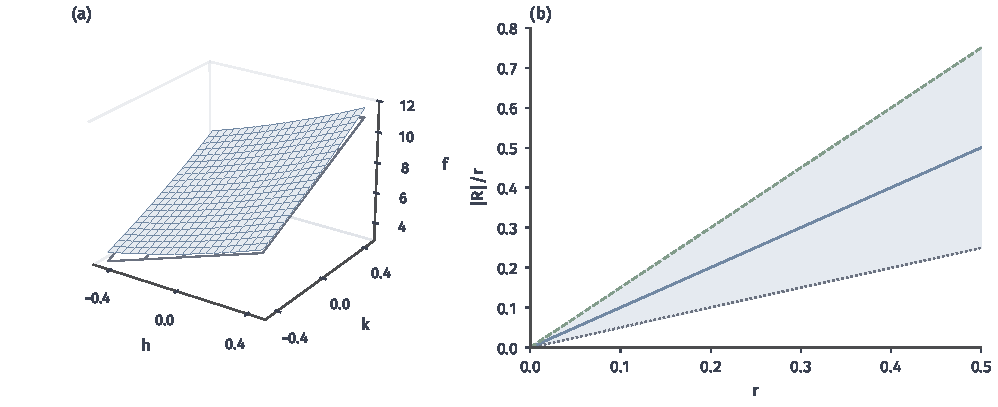
\includegraphics[width=169.0mm]{figures/01-mathematical-preliminaries-upper/01-mathematical-language-combinatorics-analysis-optimization/matplotlib/chapter3-concept-processes/total-differential-remainder.pdf}
 \caption{对二次函数在$(1,2)$处，灰网格是$P=7+4h+5k$，蓝面是$f(1+h,2+k)$。(b) 令$r=\sqrt{h^2+k^2}$，余项$R=h^2+hk+k^2$满足$r/2\leq R/r\leq3r/2$；阴影给出所有方向的完整范围，三条线是其中的代表值。共同上界随$r\to0$趋零，才保证任意方向都适用同一个线性近似。}
 \label{fig:analysis-process-total-differential-remainder}
\end{figure*}

对单位方向$\bm u$，内积不等式给出$D_{\bm u}f(\bm a)\leq\lVert\nabla f(\bm a)\rVert_2$。
当梯度非零时，在$\bm u=\nabla f(\bm a)/\lVert\nabla f(\bm a)\rVert_2$处取等号，故可微函数的梯度方向是局部上升最快的单位方向。
这个结论需要可微性，不能只由梯度向量存在推出。


图~\ref{fig:analysis-process-gradient-level-curves}用同一个二次函数比较梯度方向、等值曲线切向及另一个单位方向。
\begin{figure}[!htbp]
 \centering
 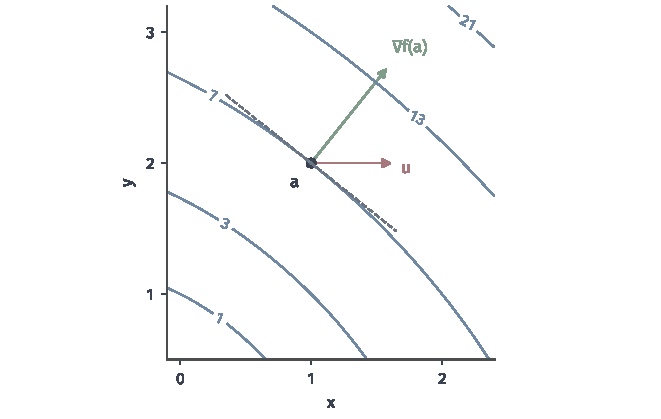
\includegraphics[width=112.0mm]{figures/01-mathematical-preliminaries-upper/01-mathematical-language-combinatorics-analysis-optimization/matplotlib/chapter3-concept-processes/gradient-level-curves.pdf}
 \caption{$f=x^2+xy+y^2$的等值曲线，标注为函数值；基点$a=(1,2)$处$\nabla f=(4,5)^\top$，图中绿箭头按$0.15$倍绘制。灰虚线沿$(5,-4)^\top$，与梯度垂直，因而与经过$a$的等值曲线相切；红箭头为$u=(1,0)^\top$。比较最快上升方向时须先归一化，不能直接比较图中箭头长度。}
 \label{fig:analysis-process-gradient-level-curves}
\end{figure}

\paragraph{偏导数连续给出的充分条件}
如果各坐标的变化率在同一点附近连续，就可以用它们共同控制全部坐标增量。
与上面的必要条件不同，这项条件可以直接保证全微分存在。
\begin{theorem}[偏导数连续与可微性]
\label{thm:multivariable-continuous-partials-sufficient}
设$f:U\to\mathbb R$，$U$开，$\bm a\in U$。若各一阶偏导数在$\bm a$的某个邻域内存在，并在$\bm a$处连续，则$f$在$\bm a$处可微。
\end{theorem}
\begin{proof}
这项条件可以沿坐标逐个改变来核对：把$\bm a$到$\bm a+\bm h$的增量拆成$d$段，
每段只改一个坐标，一元中值定理将该段增量写成相应中间点处的偏导数乘$h_j$。
当$\bm h\to\bm0$时，所有中间点都趋于$\bm a$；偏导连续性因此使
\[
 \begin{aligned}
 &\left|f(\bm a+\bm h)-f(\bm a)-\sum_{j=1}^d\partial_j f(\bm a)h_j\right|\\
 &\qquad\leq \max_j\left|\partial_j f(\bm\xi_j)-\partial_j f(\bm a)\right|
       \sum_{j=1}^d|h_j|
 =o(\lVert\bm h\rVert_2),
 \end{aligned}
\]
其中$\bm\xi_j$是第$j$段的中间点，最后一步用了$\sum_j|h_j|\leq\sqrt d\lVert\bm h\rVert_2$。
这就把各坐标上的变化拼成了同一个有效的全微分。
\end{proof}
偏导数连续只是充分条件。可微仅要求函数增量具有统一的一阶近似，不要求这些系数随基点连续变化。

\paragraph{连续可微函数}
若还希望各点的一阶系数连续变化，就需在一个范围内同时控制偏导数。
实值函数的各一阶偏导数在开集$U$上存在且连续时，称它在$U$上连续可微，记为$C^1(U)$；$C^k(U)$表示直至$k$阶的各偏导数都存在且连续。
刚才的充分条件保证$C^1$函数处处可微，逆向并不成立。

\paragraph{条件之间的蕴含关系}
由必要条件与充分判别，现在可以把这些要求放在一起比较：
\[
 \begin{gathered}
 f\text{在}\bm a\text{的某邻域内连续可微}
 \ \Longrightarrow\ f\text{在}\bm a\text{处可微},\\
 f\text{在}\bm a\text{处可微}
 \ \Longrightarrow\ \text{全部双侧方向导数存在}
 \ \Longrightarrow\ \text{全部偏导数存在}.
 \end{gathered}
\]
第一条已由连续偏导数的充分判别得到，第二条已由必要条件定理证明，最后只须在全部方向中取坐标方向$\bm e_j$。
可微还蕴含连续，并使方向导数关于方向成为同一个线性映射；相应公式已在必要条件中给出。
首项要求一个邻域内偏导数连续，其余各项只约束同一基点；即使要求处处可微，也不能反推连续可微。
一元函数的普通导数存在就等价于可微，多元函数则还须协调多个输入方向，所以上面各条逆命题需要分别检验。

\paragraph{偏导数存在不保证可微}
下面检验蕴含链中的逆命题。先看坐标偏导数：它们只约束坐标切片，并未控制其余方向或路径。
\begin{example}[偏导数存在但不可微]
\label{ex:analysis-partials-not-differentiable}
定义$f:\mathbb{R}^2\to\mathbb{R}$为
\[   f(x,y)=
\begin{cases}     \dfrac{xy}{\sqrt{x^2+y^2}}, & (x,y)\neq(0,0),\\[6pt]     0, & (x,y)=(0,0).
\end{cases} \]
沿两条坐标轴，函数恒为$0$，所以 $\partial f/\partial x(0,0)=\partial f/\partial y(0,0)=0$。若$f$在原点可微， 候选线性部分只能是零映射。可是沿$\bm{h}=(t,t)$，
\[   \frac{|f(t,t)-f(0,0)|}{\lVert(t,t)\rVert_2}   =   \frac{|t|/\sqrt{2}}{\sqrt{2}|t|}   =\frac12, \]
余项与$\lVert\bm{h}\rVert_2$之比不趋于零，故$f$在原点不可微。偏导数只看坐标轴，遗漏了其他接近路径。本例沿每个方向$\bm v=(a,b)$的
正向方向导数都存在，这里只令$t\downarrow0$，得到$ab/\sqrt{a^2+b^2}$（零方向取$0$）；它却不是关于$\bm v$
的线性函数，而且双侧方向导数在$ab\neq0$时不存在。方向极限采用单侧还是双侧，
必须与所用定义一致；本节定义采用双侧极限。
本例还在原点连续，因为$|xy|/\sqrt{x^2+y^2}\leq\sqrt{x^2+y^2}/2$；所以补上连续性也不能反推可微。
\end{example}

\paragraph{全部方向导数存在不保证可微}
从坐标切片扩展到所有固定直线，仍需检查这些变化率能否组成线性映射，以及是否具有统一余项。先看缺少线性性的情形，令
$g(x,y)=x^3/(x^2+y^2)$于非零点，$g(0,0)=0$。
沿$\bm v=(a,b)\neq\bm0$有$D_{\bm v}g(0,0)=a^3/(a^2+b^2)$，
但坐标方向导数给出的候选梯度为$(1,0)^\top$，它对方向$(1,1)^\top$
预测$1$而非实际的$1/2$。这些方向变化率无法拼成一个线性映射。
与前例的单侧方向极限相比，这里直接检验了本节采用的双侧定义。

\begin{example}[所有方向导数为零仍不足以可微]
\label{ex:multivariable-linear-directionals-not-differentiable}
前面的双侧方向导数反例不能组成线性函数。即使补上这一要求，仍需检查统一余项。
在非原点处令$q(x,y)=x^3y/(x^4+y^2)$，并令$q(0,0)=0$。
由$2|x^2y|\leq x^4+y^2$，有$|q(x,y)|\leq|x|/2$，故$q$在原点连续。
对固定方向$(a,b)^\top$，若$b\neq0$，
\[
 \frac{q(ta,tb)}t=\frac{t a^3b}{t^2a^4+b^2}\longrightarrow0;
\]
若$b=0$，差商恒为零。因此所有双侧方向导数都为零，它们也组成零线性映射。
可是沿$\bm h=(t,t^2)^\top$，$q(t,t^2)=t/2$，从而
\[
 \frac{|q(t,t^2)|}{\lVert(t,t^2)\rVert_2}
 =\frac1{2\sqrt{1+t^2}}\longrightarrow\frac12.
\]
候选零映射不能满足全微分的余项条件。方向导数先固定方向再取极限，
全微分则要求对方向随扰动改变的序列也有同一个误差控制。
\end{example}

\paragraph{可微不保证连续可微}
一元函数已经足以否定这个逆命题。在实轴上令$r(0)=0$，$x\neq0$时令$r(x)=x^2\sin(1/x^2)$。
由于$r(h)/h=h\sin(1/h^2)\to0$，有$r'(0)=0$；非零点按运算法则求导得到
\[
 r'(x)=2x\sin(1/x^2)-\frac{2}{x}\cos(1/x^2).
\]
取$x_n=(2\pi n)^{-1/2}$，有$r'(x_n)=-2/x_n\to-\infty$，所以$r'$在$0$处不连续，$r$却处处可微。
在多元情形令$f(\bm x)=r(x_1)$，同样得到处处可微而非连续可微的标量函数。
这个例子还说明可微不保证局部Lipschitz：若原点邻域内有共同Lipschitz常数，那里每个已存在的一元导数都应被这个常数控制，与上述无界导数矛盾。

\paragraph{连续不保证偏导数存在}
反方向也不能从连续性补回微分条件。
例如$f(x,y)=|x|$在整个平面上Lipschitz连续，但原点关于$x$的双侧偏导数不存在，因此在那里不可微。
反向也失败：例~\ref{ex:multivariable-path-limits}中原点置零的$xy/(x^2+y^2)$沿坐标轴恒零，两个偏导数存在，但原点不连续。
因此连续与偏导数存在之间没有一般单向蕴含；可微则能够同时保证二者。

\paragraph{梯度与线性近似的使用条件}
上述反例区分了两种用途：仅有偏导数时，梯度只是坐标变化率排成的向量；确认可微以后，才可用它统一预测增量，并用内积计算任意方向导数。
连续偏导数提供方便的充分判别，却不是必要条件；不满足该判别时，应回到全微分的统一余项定义检查。
后面讨论向量值函数时，将对各个标量输出分量分别检查，再组成Jacobian及复合微分。

\subsubsection{微分的运算法则}

以下$f,g$都在同一开集内定义，并在基点$\bm a$处可微，$c$为固定实数。
将各自的一阶展开相加或相乘，比较线性项与高阶余项，就能逐项得到下面的法则。

\paragraph{和的微分}
函数相加时，一阶近似相加，因此
\[
 \mathrm d(f+g)=\mathrm df+\mathrm dg.
\]
右侧微分在同一基点作用于同一个扰动，两个$o(\lVert\bm h\rVert_2)$余项相加后仍满足可微性要求。

\paragraph{差的微分}
函数相减时，一阶近似相减，因此
\[
 \mathrm d(f-g)=\mathrm df-\mathrm dg.
\]
余项之差仍为$o(\lVert\bm h\rVert_2)$，所以差函数也可微。

\paragraph{数乘的微分}
固定系数只会缩放线性项与余项，故$\mathrm d(cf)=c\,\mathrm df$，包括$c=0$的常函数情形。

\paragraph{积的微分}
展开$(f(\bm a)+\mathrm df(\bm h)+o(\lVert\bm h\rVert_2))(g(\bm a)+\mathrm dg(\bm h)+o(\lVert\bm h\rVert_2))$，保留一次项，得到
\[
 \mathrm d(fg)=g(\bm a)\,\mathrm df+f(\bm a)\,\mathrm dg.
\]
两个线性增量的乘积为$O(\lVert\bm h\rVert_2^2)$，可并入一阶余项，故该计算确实证明乘积可微。

\paragraph{商的微分}
若$g(\bm a)\neq0$，连续性保证邻近分母远离零。一元倒数函数的展开给出$\mathrm d(1/g)=-\mathrm dg/g(\bm a)^2$，再用积法则得到
\[
 \mathrm d(f/g)=\frac{g(\bm a)\,\mathrm df-f(\bm a)\,\mathrm dg}{g(\bm a)^2}.
\]
这里分母非零是定义商函数及估计余项的共同条件。

\paragraph{标量复合函数的微分}
若一元函数$\psi$在$f(\bm a)$处可微，且复合在邻域内有定义，将$f$的增量代入$\psi$的一元展开得到
\[
 \mathrm d(\psi\circ f)=\psi'(f(\bm a))\,\mathrm df.
\]
因为$f(\bm a+\bm h)-f(\bm a)=O(\lVert\bm h\rVert_2)$，外层的一阶余项仍是$o(\lVert\bm h\rVert_2)$。

\paragraph{二次型的微分}
向量自变量的二次型仍是标量函数，有限和的乘积法则可以直接用于它。考虑$q(\bm{x})=\bm{x}^{\top}\bm{A}\bm{x}$，其中 $\bm{A}\in\mathbb{R}^{d\times d}$固定。由乘积法则，
\begin{align*}
  \mathrm{d}q
  &=
  (\mathrm{d}\bm{x})^{\top}\bm{A}\bm{x}
  +\bm{x}^{\top}\bm{A}\,\mathrm{d}\bm{x}\\
  &=
  \bm{x}^{\top}(\bm{A}^{\top}+\bm{A})\,\mathrm{d}\bm{x}.
\end{align*}
因此
\begin{equation}
  \nabla_{\bm{x}}
  \bigl(\bm{x}^{\top}\bm{A}\bm{x}\bigr)
  =
  (\bm{A}+\bm{A}^{\top})\bm{x}.
\label{eq:analysis-quadratic-form-gradient}
\end{equation}
只有当$\bm{A}$对称时才能化为$2\bm{A}\bm{x}$。直接写成$2\bm{A}\bm{x}$会悄然加入对称性条件。

\subsubsection{中值定理与Lipschitz条件}

导数控制一点处的变化；若连接两点的整条线段都在定义域内，可以沿线段使用一元中值定理，得到有限增量的结论。
\begin{theorem}[多元标量函数的中值公式]
\label{thm:multivariable-scalar-mean-value}
设$f$在包含$[\bm x,\bm y]$的开集上可微，$\bm x\neq\bm y$。则存在$\theta\in(0,1)$使
\[
 f(\bm y)-f(\bm x)=\nabla f(\bm x+\theta(\bm y-\bm x))^\top(\bm y-\bm x).
\]
特别地，若沿线段有$\lVert\nabla f\rVert_2\leq L$，则$|f(\bm y)-f(\bm x)|\leq L\lVert\bm y-\bm x\rVert_2$。
\end{theorem}
\begin{proof}
令$\phi(t)=f(\bm x+t(\bm y-\bm x))$。由方向导数公式，$\phi'(t)=\nabla f(\bm x+t(\bm y-\bm x))^\top(\bm y-\bm x)$。
对$\phi$使用一元中值定理得到等式，再用内积不等式得到增量界。
\end{proof}
如果定义域是凸开集且各点梯度范数都不超过同一个有限$L$，任意两点间的线段都在域内，故$f$在全域满足Lipschitz条件。
局部邻域上有这样的界时得到局部Lipschitz条件；不能忽略连接线段是否属于定义域。

特别地，若$f\in C^1(U)$，在每个基点附近取一个包含在$U$内的闭球，连续梯度在球上有界，球内线段也不离开球，故上述估计保证$f$局部Lipschitz。
这不自动给出全域共同常数：实轴上的$x^2$连续可微，但其梯度在全域无界，因而不是全域Lipschitz函数。

\subsection{多元标量函数的高阶微分}
\label{sec:multivariable-curvature-error}

一阶微分记录局部线性变化，高阶微分进一步说明这些系数怎样变化。
下面先把二阶偏导数集中为Hessian矩阵，再用Taylor公式建立二阶近似，最后据此判断驻点的局部极值类型。

\subsubsection{二阶偏导数与Hessian矩阵}

一阶偏导数本身仍是多元标量函数，可以再次求偏导。这里记$f_{x_i x_j}=\partial_j(\partial_i f)$，即先对$x_i$、再对$x_j$求导。
对$f(x,y)=x^2+xy+y^2$，有$f_{xx}=2$、$f_{xy}=f_{yx}=1$、$f_{yy}=2$。一般函数的混合偏导数能否交换，需要额外条件。

\paragraph{混合偏导数的交换}
分别沿两个坐标求导时，先后次序未必自动无关。下面的连续性条件可以把两种次序联系起来。
\begin{theorem}[混合偏导数的交换]
\label{thm:multivariable-mixed-partials}
设$f$在$\bm a$的某个开邻域内有一阶偏导数$\partial_i f,\partial_j f$，混合偏导数$\partial_j\partial_i f,\partial_i\partial_j f$在该邻域存在并在$\bm a$处连续，则
\[
 \partial_j\partial_i f(\bm a)=\partial_i\partial_j f(\bm a).
\]
特别地，$C^2$函数的混合偏导数处处可以交换。
\end{theorem}
\begin{proof}
固定其他坐标，只需讨论二元函数在$(a,b)$处的情形。对小的非零$h,k$考察二阶差分
\[
 \Delta(h,k)=f(a+h,b+k)-f(a+h,b)-f(a,b+k)+f(a,b).
\]
令$\phi(x)=f(x,b+k)-f(x,b)$。先对$\phi$用一元中值定理，再对$y\mapsto f_x(\xi,y)$使用一次中值定理，得到
\[
 \Delta=h[f_x(\xi,b+k)-f_x(\xi,b)]=hk f_{xy}(\xi,\eta),
\]
其中$\xi$在$a,a+h$之间、$\eta$在$b,b+k$之间。先沿$y$方向拆分则得到$\Delta=hk f_{yx}(\xi',\eta')$。
除以$hk$后令$h,k\to0$，各中间点趋于$(a,b)$，连续性使两种混合偏导数在该点相等。
\end{proof}
只有偏导数存在而没有这些连续性条件时，结论可能失败。

\paragraph{Hessian矩阵}
把各偏导数的坐标变化率集中起来，就得到记录二阶信息的矩阵。
它的行、列分别对应先后两次求导的输入坐标。
\begin{definition}[Hessian矩阵]
\label{def:multivariable-hessian}
若$f:U\to\mathbb R$在$\bm x$附近有一阶偏导数，且各$\partial_j\partial_i f(\bm x)$存在，则称
\[
 \nabla^2f(\bm x)=\bigl[\partial_j\partial_i f(\bm x)\bigr]_{i,j=1}^d
\]
为$f$在该点的\term{Hessian矩阵}（Hessian matrix）。
\end{definition}
二阶偏导数存在本身尚不保证一阶导数具有统一的线性近似；二阶可微要求一阶导数映射本身可微。
$C^2$是保证二阶可微的充分条件，且此时Hessian对称。对上面的二次函数，Hessian就是$\begin{bmatrix}2&1\\1&2\end{bmatrix}$。
若$f\in C^2$，沿直线$t\mapsto f(\bm x+t\bm v)$求两次导数，在$t=0$处得到
\[
 \bm v^\top\nabla^2f(\bm x)\bm v
 =\sum_{i=1}^d\sum_{j=1}^d \partial_j\partial_i f(\bm x)v_i v_j.
\]
这个实数二次型衡量沿给定方向的一阶斜率变化。

对二次函数
\[   f(\bm{x})   =   \frac12\bm{x}^{\top}\bm{A}\bm{x}   +\bm{b}^{\top}\bm{x}+c, \]
只有$\bm{A}$的对称部分影响函数值。令 $\bm{H}=(\bm{A}+\bm{A}^{\top})/2$，则 $\nabla f(\bm{x})=\bm{H}\bm{x}+\bm{b}$且 $\nabla^2f(\bm{x})=\bm{H}$。
例如$\bm H=\operatorname{diag}(2,100)$时，方向二次型为$2v_1^2+100v_2^2$，
沿两个坐标方向都向上弯，但第二个方向的二阶变化率是第一个的$50$倍。
若改为$\operatorname{diag}(2,-100)$，两个坐标方向的弯曲方向便相反。
判断曲率需要检查整个二次型，而不是某一个对角元素。

对实对称矩阵$\bm H$，若每个非零$\bm v$都有$\bm v^\top\bm H\bm v>0$，称$\bm H$正定；
若只要求$\bm v^\top\bm H\bm v\geq0$，则称半正定。
把不等号反向得到负定与半负定；若既存在使二次型为正的方向，又存在使它为负的方向，
则称矩阵不定。这些名称分别说明全部方向或某些方向上的曲率符号。



\subsubsection{Taylor公式与局部近似}

把多个坐标同时改变的位移写成一条线段上的参数变化，就能回用一元Taylor公式。
下述公式都针对标量输出，二阶项是一个实数二次型。

一元Taylor定理可沿整条位移线段使用，而基点附近的连续二阶偏导数进一步给出小量形式的余项。
\begin{theorem}[多元标量函数的二阶Taylor公式]
\label{thm:multivariable-second-order-taylor}
设$f\in C^2(U)$，$U\subseteq\mathbb R^d$开，线段$[\bm x,\bm x+\bm h]\subset U$。若$\bm h\neq0$，则存在$\theta\in(0,1)$使
\begin{equation}
 f(\bm x+\bm h)=f(\bm x)+\nabla f(\bm x)^\top\bm h
 +\frac12\bm h^\top\nabla^2f(\bm x+\theta\bm h)\bm h.
\label{eq:analysis-second-order-taylor}
\end{equation}
对固定$\bm x\in U$，当$\bm h\to0$时还有
\begin{equation}
 f(\bm x+\bm h)=f(\bm x)+\nabla f(\bm x)^\top\bm h
 +\frac12\bm h^\top\nabla^2f(\bm x)\bm h+o(\lVert\bm h\rVert_2^2).
\label{eq:analysis-second-order-local-model}
\end{equation}
\end{theorem}
\begin{proof}
令$\phi(t)=f(\bm x+t\bm h)$。由一阶微分公式，$\phi'(t)=\nabla f(\bm x+t\bm h)^\top\bm h$；再对各偏导数沿线段求导，得$\phi''(t)=\bm h^\top\nabla^2f(\bm x+t\bm h)\bm h$。
对$\phi$使用一元Taylor定理即得第一式。矩阵各元素的连续性保证
$\lVert\nabla^2f(\bm x+\theta\bm h)-\nabla^2f(\bm x)\rVert_F\to0$，其中$0<\theta<1$可以随$\bm h$变化。
由$|\bm h^\top\bm B\bm h|\leq\lVert\bm B\rVert_F\lVert\bm h\rVert_2^2$，替换Hessian产生的误差为$o(\lVert\bm h\rVert_2^2)$，得到第二式。上述不等式可对$\sum_{i,j}B_{i,j}h_i h_j$使用有限和的Cauchy--Schwarz不等式验证。
\end{proof}
例如$f(x,y)=e^{x+y}$在原点有函数值$1$、梯度$(1,1)^\top$和各元素均为$1$的Hessian。因此
\[
 e^{h+k}=1+h+k+\frac12(h+k)^2+o(h^2+k^2).
\]
一次项描述切平面，二次项补上沿位移方向的弯曲。

式~\eqref{eq:analysis-second-order-local-model}是局部结论。若要在一个区域内给出统一余项界，还需控制该区域上的Hessian矩阵连续性或Lipschitz常数，不能仅凭一点处的二阶导数。

若希望保留整条位移线段上的曲率，可以直接使用一元Taylor积分余项式~\eqref{eq:analysis-taylor-integral-remainder}。
在同一$C^2$条件下，令$\phi(t)=f(\bm x+t\bm h)$，取该式的$r=1$；刚才已计算出$\phi'$与$\phi''$，代入后得到不挑选中间点的Taylor积分余项：
\[   f(\bm{x}+\bm{h})   =   f(\bm{x})   +\nabla f(\bm{x})^{\top}\bm{h}   +   \int_0^1(1-t)   \bm{h}^{\top}\nabla^2f(\bm{x}+t\bm{h})\bm{h}\,\mathrm{d}t. \]
权重$1-t$说明越靠近位移起点的曲率贡献被累计得越多；该表达式与前面的中间点余项
描述同一有限变化，但保留了整条线段上的曲率信息。

\subsubsection{局部极值的判别}

Taylor公式已经控制线性项以外的误差，因此现在可以将梯度与Hessian的条件转化为原函数的极值结论。
局部极小点是指存在一个相对邻域，使其中所有函数值都不小于基点值；其他点均严格更大时称严格局部极小点，极大点用反向不等式定义。
本小节考察无约束开集内部的点。

\paragraph{局部极值的一阶必要条件}
沿任意方向限制成一元函数后，内部极值点仍必须满足Fermat条件。
这给出与一元导数为零相对应的向量条件。
\begin{theorem}[局部极值的一阶必要条件]
\label{thm:multivariable-extremum-first-order}
设$f$在开集内部点$\bm x^\star$处可微，且该点为局部极小点或局部极大点，则
\begin{equation}
 \nabla f(\bm x^\star)=\bm0.
\label{eq:analysis-first-order-necessary}
\end{equation}
\end{theorem}
\begin{proof}
对每个方向$\bm v$，一元函数$t\mapsto f(\bm x^\star+t\bm v)$在$0$处有局部极值，故导数$\nabla f(\bm x^\star)^\top\bm v=0$。
取各坐标方向，即得全部偏导数为零。
\end{proof}
梯度为零的点称为驻点；驻点未必是极值点。

\paragraph{局部极值的二阶必要条件}
如果邻域内还具有连续二阶偏导数，则任一方向上的一元二阶导数还要具有相应的符号。
\begin{theorem}[局部极值的二阶必要条件]
\label{thm:multivariable-extremum-second-order}
设$f$在$\bm x^\star$附近属于$C^2$。若$\bm x^\star$为内部局部极小点，则
\begin{equation}
 \bm v^\top\nabla^2f(\bm x^\star)\bm v\geq0
 \qquad(\bm v\in\mathbb R^d),
\label{eq:analysis-second-order-necessary}
\end{equation}
即Hessian半正定；内部局部极大点对应Hessian半负定。
\end{theorem}
\begin{proof}
对$t\mapsto f(\bm x^\star+t\bm v)$使用一元极值的二阶必要条件，其二阶导数正是所述二次型。
\end{proof}
必要条件不能单独决定驻点类型。一元函数$x^4$、$-x^4$及$x^3$在$0$处一阶、二阶导数都为零，却分别为极小、极大和非极值；多元函数在二次型退化的方向上同样要检查更高阶项。

\paragraph{驻点的二阶充分条件}
若各非零方向的二次型都有严格符号，Taylor余项便不会改变充分小扰动下的函数增量符号。
\begin{theorem}[驻点的Hessian判别]
\label{thm:multivariable-hessian-classification}
设$f$在$\bm x^\star$附近属于$C^2$，且$\nabla f(\bm x^\star)=0$。
若Hessian正定，则$\bm x^\star$是严格局部极小点；若负定，则为严格局部极大点；若不定，则任意小邻域都存在函数值大于及小于$f(\bm x^\star)$的点。
\end{theorem}
\begin{proof}
正定Hessian矩阵给出更强的充分条件：它要求每个方向都有正曲率，而不只是没有负曲率。
设$f$在$\bm{x}^{\star}$的某个邻域内二阶连续可微，
$\nabla f(\bm{x}^{\star})=\bm{0}$且
$\bm H_\star=\nabla^2f(\bm{x}^{\star})$正定。要把各方向的正曲率变成同一个正下界，
可以在闭有界的单位球面上考察连续函数$\bm v\mapsto\bm v^\top\bm H_\star\bm v$。
由闭有界集上的极值定理，它取到最小值
\[
 \lambda=\min_{\lVert\bm v\rVert_2=1}\bm v^\top\bm H_\star\bm v>0.
\]
正定性保证取到的值仍为正。把任意非零$\bm h$除以其长度，就得到
$\bm h^\top\bm H_\star\bm h\geq\lambda\lVert\bm h\rVert_2^2$。
由Hessian矩阵的连续性，在足够小的球内有
$\lVert\nabla^2f(\bm x)-\bm H_\star\rVert_F\leq\lambda/2$；
Frobenius范数因而把二次型的变化量控制在$(\lambda/2)\lVert\bm h\rVert_2^2$以内，
邻近位置的曲率下界仍至少为$(\lambda/2)\lVert\bm h\rVert_2^2$。
用式~\eqref{eq:analysis-second-order-taylor}
的中间点表达式，即可把这个曲率下界变成函数值下界；具体地，充分靠近时有
\[   f(\bm{x}^{\star}+\bm{h})-f(\bm{x}^{\star})   \geq   \frac{\lambda}{4}\lVert\bm{h}\rVert_2^2>0 \]
对充分小的非零$\bm{h}$成立，故$\bm{x}^{\star}$是严格局部极小点。负定情形给出严格局部极大点。

若驻点处Hessian矩阵不定，分别选取二次型为正和为负的方向。
沿每个固定方向把扰动写成$t\bm v$时，余项为$o(t^2)$，因此充分小的非零$t$不会改变
非零二次项的符号，函数值因而分别增加和减小，该点称为\term{鞍点}（saddle point）。
例如$f(x,y)=x^2-y^2$的原点就是鞍点。
若Hessian矩阵仅半正定或半负定，且在某些非零方向上二次型为零，二阶判据可能没有结论，
必须查看更高阶项或函数的其他结构。上述必要条件还假定点位于无约束开集内部；
边界极小点的梯度可以不为零，受约束问题需要后续章节的可行方向与乘子条件。
\end{proof}


图~\ref{fig:analysis-process-hessian-local-shapes}对照二阶判别可以决定的形状，以及Hessian退化时仍需继续检查的情形。
\begin{figure*}[!htbp]
 \centering
 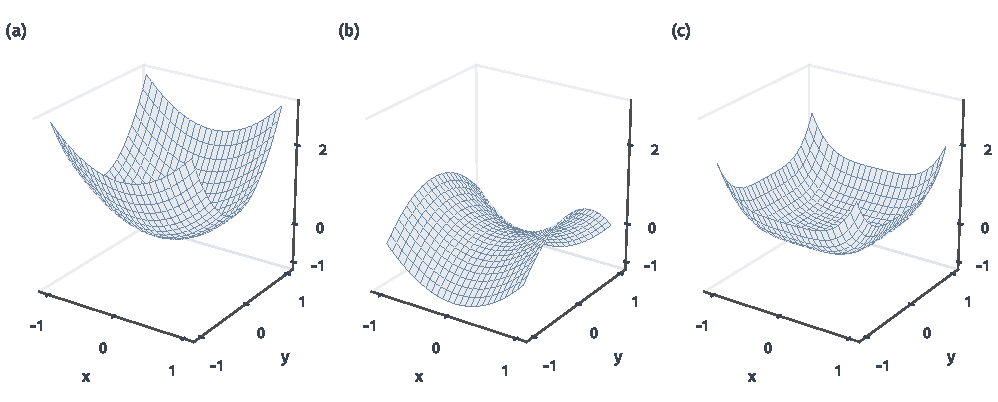
\includegraphics[width=169.0mm]{figures/01-mathematical-preliminaries-upper/01-mathematical-language-combinatorics-analysis-optimization/matplotlib/chapter3-concept-processes/hessian-local-shapes.pdf}
 \caption{同一$[-1,1]^2$范围和纵轴尺度下，三面分别为$x^2+2y^2$、$x^2-y^2$、$x^4+y^4$。原点的Hessian依次为正定、不定、零矩阵；前两者给严格极小与鞍点，第三者虽严格极小却不能由正定判据推出。零Hessian也可能没有极值，例如前述$x^3$，故退化不是一种确定分类。}
 \label{fig:analysis-process-hessian-local-shapes}
\end{figure*}

\FloatBarrier

\subsection{多元向量值函数的微分}

前面每个输入只产生一个实数。现在固定$F:U\subseteq\mathbb R^d\to\mathbb R^m$，同一输入同时产生$m$个输出分量；参数曲线与曲面也是这种映射的特殊情况。
有限个输出可以逐分量检查，但输入仍要整体扰动，不能以坐标切片代替各分量的全微分。

\subsubsection{向量值函数及其极限与连续性}

给出所有输出分量，就确定了整个映射；因此先按输出分量组织其表示。
\begin{definition}[多元向量值函数]
\label{def:multivariable-vector-function}
映射$F:U\subseteq\mathbb R^d\to\mathbb R^m$称为多元向量值函数，写作$F=(F_1,\ldots,F_m)^\top$，其中每个$F_i:U\to\mathbb R$为多元标量函数。
\end{definition}
其极限与连续性使用输出欧氏距离$\lVert F(\bm x)-\bm b\rVert_2$。
对有限个输出，这等价于每个$F_i$的对应极限存在或在同一基点连续，因为
\[
 \max_i|F_i(\bm x)-b_i|\leq\lVert F(\bm x)-\bm b\rVert_2
 \leq\sqrt m\max_i|F_i(\bm x)-b_i|.
\]
这里分解的是输出分量，区别于只沿某些输入坐标检查的切片。

\subsubsection{微分与Jacobian矩阵}

标量输出使用到实数的线性映射，也称线性泛函；向量输出则需要把输入扰动映射为$m$维输出扰动。
有限维线性映射由矩阵表示，矩阵的每一行记录一个输出分量的系数。
\begin{definition}[向量值函数的微分]
\label{def:multivariable-vector-differential}
设$U$开，$F:U\to\mathbb R^m$，$\bm a\in U$。若存在矩阵$\bm J_F(\bm a)\in\mathbb R^{m\times d}$，使
\begin{equation}
 F(\bm a+\bm h)=F(\bm a)+\bm J_F(\bm a)\bm h+o(\lVert\bm h\rVert_2),
\label{eq:analysis-jacobian-linearization}
\end{equation}
则称$F$在$\bm a$处可微，余项按输出欧氏范数理解。
其微分为$\mathrm dF_{\bm a}(\bm h)=\bm J_F(\bm a)\bm h$，其中$\bm J_F$称为\term{Jacobian矩阵}（Jacobian matrix），第$i,j$个元素为$\partial_jF_i$。
\end{definition}
向量值函数可微当且仅当每个输出分量$F_i$可微：正向可从向量余项取分量，反向则将有限个分量的$o(\lVert\bm h\rVert_2)$余项用欧氏范数合并。
因此Jacobian的第$i$行是标量分量梯度$\nabla F_i^\top$；$m=1$时Jacobian是梯度的转置，而不是梯度列向量本身。
$C^k$向量值函数指所有输出分量都属于$C^k$。


图~\ref{fig:analysis-process-jacobian-grid-cell}把向量值映射的线性近似画成小网格块的变化。后面区域换元还会使用这个局部矩阵的行列式。
\begin{figure*}[!htbp]
 \centering
 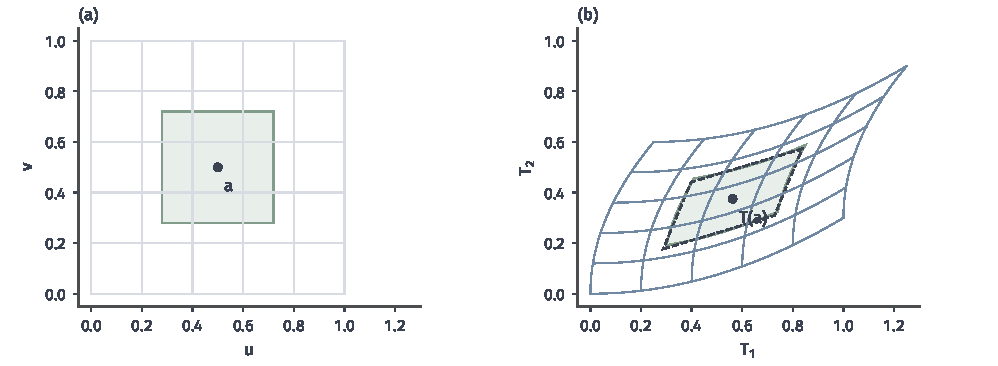
\includegraphics[width=169.0mm]{figures/01-mathematical-preliminaries-upper/01-mathematical-language-combinatorics-analysis-optimization/matplotlib/chapter3-concept-processes/jacobian-grid-cell.pdf}
 \caption{取$T(u,v)=(u+v^2/4,\,0.6v+0.3u^2)$，$a=(0.5,0.5)$。(a) 输入网格及绿色小方块。(b) 非线性像为弯边块，黑虚线为$T(a)+J_T(a)(h,k)^\top$给出的平行四边形；$J_T(a)=\bigl[\begin{smallmatrix}1&0.25\\0.3&0.6\end{smallmatrix}\bigr]$。有限块不与线性像完全重合，缩小扰动后才由可微余项控制差异。}
 \label{fig:analysis-process-jacobian-grid-cell}
\end{figure*}

\paragraph{Jacobian矩阵的计算}
每个输出先按标量函数求偏导，再按行排列，可以核对输入、输出与矩阵形状是否一致。
例如$F(x,y)=(x^2+xy,y^2)^\top$的Jacobian为
\[
 \bm J_F(x,y)=\begin{bmatrix}2x+y&x\\0&2y\end{bmatrix}.
\]
在$(1,2)$处，它把扰动$(h,k)^\top$的一阶影响写成$(4h+k,4k)^\top$。两个输出分别占一行，两个输入分别占一列。

若要把任意实数组变成正数且总和为$1$的权重，可以先取指数再除以共同的总和。
这就是$n$维\term{归一化指数映射}（softmax）。对正整数$n$和
$\bm{z}\in\mathbb{R}^n$，令
\[
  s_i(\bm{z})
  =
  \frac{e^{z_i}}{\sum_{k=1}^n e^{z_k}},
  \qquad i=1,\ldots,n.
\]
记分母为$Z=\sum_k e^{z_k}$。指数函数求导和商法则给出
\[
  \frac{\partial s_i}{\partial z_j}
  =
  \frac{\mathbb{I}\{i=j\}e^{z_i}Z-e^{z_i}e^{z_j}}{Z^2}
  =
  s_i\bigl(\mathbb{I}\{i=j\}-s_j\bigr).
\]
因此整个Jacobian矩阵为
\begin{equation}
  \bm{J}_{\bm{s}}(\bm{z})
  =
  \operatorname{diag}(\bm{s})-\bm{s}\bm{s}^{\top}.
\label{eq:analysis-softmax-jacobian}
\end{equation}
这里$\operatorname{diag}(\bm s)$表示以$s_1,\ldots,s_n$为对角元、其他元素为零的对角矩阵。
对角项$s_i(1-s_i)$描述提高$z_i$对自身分量的影响，非对角项$-s_is_j$
来自共同分母：提高一个坐标会压低其余归一化分量。每行元素之和为零，
这也与给所有$z_i$同时加同一常数不改变输出相符。



\subsubsection{向量值函数的微分运算}
\label{sec:analysis-vector-chain-matrix-calculus}

运算必须先有定义。相同形状的向量输出可以相加、相减和数乘；复合则要求前一映射的输出属于后一映射的定义域。
这里不把没有指定乘法含义的两个向量直接套入标量乘积法则。

\paragraph{和的微分}
若$F,H:U\to\mathbb R^m$在$\bm a$处可微，则逐分量使用和法则，得到
\[
 \bm J_{F+H}(\bm a)=\bm J_F(\bm a)+\bm J_H(\bm a).
\]
相加的输出形状以及两个Jacobian的形状必须分别一致。

\paragraph{差的微分}
在相同条件下，逐分量使用差法则，得到
\[
 \bm J_{F-H}(\bm a)=\bm J_F(\bm a)-\bm J_H(\bm a).
\]

\paragraph{数乘的微分}
对固定实数$c$，逐分量使用数乘法则，得到
\[
 \bm J_{cF}(\bm a)=c\bm J_F(\bm a).
\]

\paragraph{复合函数的链式法则}
前一映射产生的输出扰动，还要经过后一映射的线性响应。
因此复合微分按实际计算顺序组合，Jacobian的乘法次序由输入与输出维度决定。
\begin{theorem}[向量值函数的链式法则]
\label{thm:multivariable-vector-chain-rule}
设$U\subseteq\mathbb R^d$、$V\subseteq\mathbb R^m$开，$F:U\to V$在$\bm a$处可微，$G:V\to\mathbb R^p$在$F(\bm a)$处可微，则$G\circ F$在$\bm a$处可微，且
\begin{equation}
 \bm J_{G\circ F}(\bm a)=\bm J_G(F(\bm a))\bm J_F(\bm a).
\label{eq:analysis-vector-chain-rule}
\end{equation}
\end{theorem}
\begin{proof}
记$\bm A=\bm J_F(\bm a)$、$\bm B=\bm J_G(F(\bm a))$，由$F$可微有$\bm k=F(\bm a+\bm h)-F(\bm a)=\bm A\bm h+o(\lVert\bm h\rVert_2)$，故$\lVert\bm k\rVert_2=O(\lVert\bm h\rVert_2)$。
代入$G$的一阶展开得到$G(F(\bm a)+\bm k)-G(F(\bm a))=\bm B\bm A\bm h+o(\lVert\bm h\rVert_2)$，其中外层余项$o(\lVert\bm k\rVert_2)$也被原扰动尺度控制。
这正是复合函数的可微定义。
\end{proof}
矩阵形状为$(p\times m)(m\times d)=p\times d$，反向相乘往往没有定义。
即使两个次序都有定义，矩阵乘法一般也不交换，不能按标量经验调换因子。这项复合规则称为\term{链式法则}（chain rule）。

\paragraph{标量复合函数的梯度}

前面的外层映射$G$允许向量输出。当$p=1$时，它把中间向量变成一个标量。在优化问题中，
这个标量通常是待最小化的目标值，本书便把此时的$G$记为$\ell$。令
$\bm y=F(\bm x)$，总目标就是$L(\bm x)=\ell(F(\bm x))$；$\ell$只是原复合映射的
最后一层，并没有增加一个未说明的输出。采用列向量梯度，链式法则写成
\[
  \nabla L(\bm x)
  =\bm J_F(\bm x)^\top\nabla\ell(\bm y)\big|_{\bm y=F(\bm x)}.
\]
局部线性映射在前向计算中按$\bm J_F$作用，在标量目标的反向计算中按转置
$\bm J_F^\top$传回。这说明列向量梯度在复合时为何出现Jacobian的转置。


图~\ref{fig:analysis-process-chain-rule-types}把前向的函数复合与反向的梯度传递分开，便于核对转置及维度。
\begin{figure}[!htbp]
 \centering
 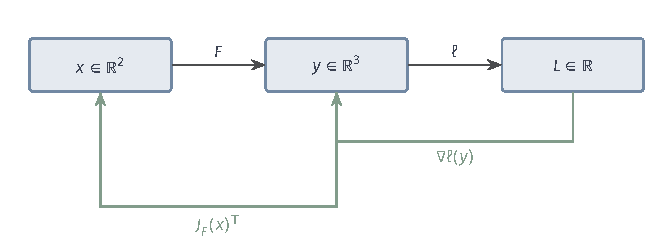
\includegraphics[width=112mm]{figures/01-mathematical-preliminaries-upper/01-mathematical-language-combinatorics-analysis-optimization/tikz/chapter3-concept-processes/chain-rule-types.pdf}
 \caption{上方是$x\in\mathbb R^2$经$F$产生$y\in\mathbb R^3$，再经$\ell$产生标量$L$。下方先得到$\nabla\ell(y)\in\mathbb R^3$，再由$2\times3$矩阵$J_F(x)^\top$传回$\nabla L(x)\in\mathbb R^2$。反向箭头表示梯度的线性传递，不表示对$F$或$\ell$求逆函数。}
 \label{fig:analysis-process-chain-rule-types}
\end{figure}

\begin{example}[从中间向量求回复合目标的梯度]
\label{ex:analysis-chain-rule-calculation}
令
\[
  F(x_1,x_2)=(x_1^2,x_1x_2,x_2)^\top,
  \qquad \ell(\bm y)=\frac12(y_1^2+y_2^2+y_3^2).
\]
$F$从二维输入产生三维中间量，$\ell$再把三维中间量变成一个数。于是
\[
  \bm J_F=\begin{bmatrix}2x_1&0\\x_2&x_1\\0&1\end{bmatrix},
  \qquad \nabla\ell(\bm y)=\bm y.
\]
在$\bm x=(1,2)^\top$处，$\bm y=(1,2,2)^\top$，链式法则给出
\[
  \nabla L(1,2)
  =\begin{bmatrix}2&2&0\\0&1&1\end{bmatrix}
    \begin{bmatrix}1\\2\\2\end{bmatrix}
  =\begin{bmatrix}6\\4\end{bmatrix}.
\]
也可以把复合函数直接展开为
$L(x_1,x_2)=\tfrac12(x_1^4+x_1^2x_2^2+x_2^2)$，求偏导得到
$\nabla L=(2x_1^3+x_1x_2^2,\,x_1^2x_2+x_2)^\top$，在同一点仍为$(6,4)^\top$。
两种计算处理同一个目标；链式形式保留了中间映射，可分别复用各层的导数。
矩阵形状$(2\times3)(3\times1)=2\times1$也核对了梯度传递的次序。
\end{example}


\subsubsection{向量增量的中值估计}

各输出分量的一元中值位置可能不同，不能保证有一个共同位置代表整个向量增量。
可以改为控制增量的范数，用线性映射的最大放大倍数估计有限变化。

\paragraph{算子范数}

对向量输出，用线性映射的最大放大倍数替代标量导数的绝对值。
\begin{definition}[欧氏诱导算子范数]
\label{def:analysis-induced-operator-norm}
对矩阵
$\bm{A}\in\mathbb{R}^{s\times r}$，由欧氏范数\term{诱导的算子范数}
（induced operator norm）定义为
\[
  \lVert\bm{A}\rVert_{\mathrm{op}}
  =
  \sup_{\bm{h}\neq\bm{0}}
  \frac{\lVert\bm{A}\bm{h}\rVert_2}{\lVert\bm{h}\rVert_2}
  =
  \sup_{\lVert\bm{h}\rVert_2=1}\lVert\bm{A}\bm{h}\rVert_2.
\]
\end{definition}
它表示线性映射对向量长度的最大放大倍数，定义立即给出
$\lVert\bm{A}\bm{h}\rVert_2
\leq\lVert\bm{A}\rVert_{\mathrm{op}}\lVert\bm{h}\rVert_2$。
例如$\bm A=\operatorname{diag}(2,1)$把第一坐标放大两倍、第二坐标保持不变，
故$\lVert\bm A\rVert_{\mathrm{op}}=2$；最大放大由第一坐标方向达到。

在含整条线段的开邻域内连续可微时，下面的范数界不要求各分量共用一个中值点。
\begin{theorem}[向量值函数的中值估计]
\label{thm:multivariable-vector-mean-value}
设$U\subseteq\mathbb R^r$开，$G:U\to\mathbb R^s$连续可微，且$[\bm y',\bm y]\subset U$，则
\begin{equation}
  \begin{aligned}
  \lVert G(\bm{y})-G(\bm{y}')\rVert_2
  &\leq
  \sup_{0\leq t\leq1}
  \left\lVert
    \bm{D}G\bigl(\bm{y}'+t(\bm{y}-\bm{y}')\bigr)
  \right\rVert_{\mathrm{op}}
  \lVert\bm{y}-\bm{y}'\rVert_2.
  \end{aligned}
\label{eq:analysis-operator-mean-value-bound}
\end{equation}
其中$\bm DG=\bm J_G$，即$G$的Jacobian矩阵。
\end{theorem}
\begin{proof}
这个向量上界无需预先使用积分公式。若$\bm u=G(\bm y)-G(\bm y')\neq\bm0$，
取单位向量$\bm v=\bm u/\lVert\bm u\rVert_2$，并沿线段定义标量函数
$\phi(t)=\bm v^\top G(\bm y'+t(\bm y-\bm y'))$。
中值定理给出某个$\tau\in(0,1)$，使
\[
 \lVert\bm u\rVert_2
 =\phi(1)-\phi(0)
 =\bm v^\top\bm DG(\bm y'+\tau(\bm y-\bm y'))(\bm y-\bm y').
\]
对右侧使用欧氏内积与算子范数的上界便得到式~\eqref{eq:analysis-operator-mean-value-bound}；
$\bm u=\bm0$时该界直接成立。
\end{proof}
若定义域为凸开集，且Jacobian的算子范数在全域不超过同一个有限$L$，则$G$为Lipschitz连续；局部球上的界给出局部版本。
特别地，若在某邻域内$L<1$，映射严格缩小任意两点间的距离。后面的隐函数构造将使用这一条件和几何尾和控制迭代。

\subsection{矩阵自变量函数的微分}

本小节的定义域$\mathcal U$均为全矩阵空间$\mathbb R^{m\times n}$中的开集，基点$\bm X\in\mathcal U$；因此全部充分小的同形扰动都允许使用。矩阵$\bm X$可以看成$mn$个实数坐标组成的输入；保留矩阵形状，能让乘法次序与迹的结构更清楚。
输出仍须分别说明：$f(\bm X)$为标量时使用矩阵梯度，$\Phi(\bm X)$为矩阵时则使用矩阵到矩阵的线性微分。

\subsubsection{矩阵标量函数的微分与梯度}

第~\ref{sec:prelim-matrix-trace}节已定义Frobenius内积与范数，满足$\langle\bm A,\bm B\rangle_F=\operatorname{tr}(\bm A^\top\bm B)$。
现在用该范数度量输入扰动，用该内积表示标量输出的一阶变化。
\begin{definition}[矩阵标量函数的梯度]
\label{def:multivariable-matrix-scalar-gradient}
设$f:\mathcal U\to\mathbb R$。若它在矩阵$\bm X$处满足
\[
 f(\bm X+\bm H)=f(\bm X)+\mathrm df_{\bm X}(\bm H)+o(\lVert\bm H\rVert_F),
\]
其中$\mathrm df_{\bm X}$为矩阵到实数的线性映射，则称$f$在该点可微。
唯一满足
\begin{equation}
 \mathrm df_{\bm X}(\bm H)=\langle\nabla_{\bm X}f,\bm H\rangle_F
 =\operatorname{tr}\bigl((\nabla_{\bm X}f)^\top\bm H\bigr)
\label{eq:analysis-matrix-gradient-definition}
\end{equation}
的同形矩阵$\nabla_{\bm X}f\in\mathbb R^{m\times n}$称为矩阵梯度。
\end{definition}
它的各元素是对相应矩阵坐标的偏导数，唯一性可逐个取只有一个非零元素的扰动检验。
计算时先用乘积法则展开微分，再利用迹的循环移位将扰动移到末端。例如乘积形状相容时，
\[
 \operatorname{tr}(\bm A\bm B)=\operatorname{tr}(\bm B\bm A),\qquad
 \operatorname{tr}(\bm A\bm B\bm C)=\operatorname{tr}(\bm B\bm C\bm A).
\]
这里循环移动的是整个因子，不能任意交换相邻矩阵。矩阵梯度的唯一性使用了全部矩阵方向；若把定义域限制在对称矩阵等子空间上，还需另行说明所用的内积与允许方向。

\paragraph{迹函数的微分}
线性迹函数已经符合定义，可以直接读出梯度。
对固定的$\bm{A}\in\mathbb{R}^{m\times n}$，令 $f(\bm{X})=\operatorname{tr}(\bm{A}^{\top}\bm{X})$。它的微分已经符合式
\eqref{eq:analysis-matrix-gradient-definition}，所以
\begin{equation}
  \nabla_{\bm{X}}\operatorname{tr}(\bm{A}^{\top}\bm{X})
  =\bm{A}.
\label{eq:analysis-trace-linear-gradient}
\end{equation}
这个简单关系常用于从迹表达式中读出梯度。

\paragraph{行列式的微分}
行列式把方阵映为一个实数，可以通过有限多项式展开来求微分。下面先在可逆矩阵处计算，便于使用行列式的乘法公式。
第~\ref{sec:prelim-determinants}节的有限多项式表达式可用来直接识别一阶项。
先设$\bm X\in\mathbb R^{d\times d}$可逆。
计算它的一阶变化，先把方向扰动$\bm H$从行列式中分离出来：
\[
 \det(\bm X+t\bm H)=\det(\bm X)\det(\bm I+t\bm X^{-1}\bm H).
\]
对固定矩阵$\bm B$，行列式的排列展开给出
$\det(\bm I+t\bm B)=1+t\operatorname{tr}(\bm B)+O(t^2)$。
其中一次项只能从恒等排列的一个对角位置选取$tB_{i,i}$，其余位置选$1$；
非恒等排列至少改变两个位置，因此只贡献二次及以上项。
行列式是有限多项式，故在固定$\bm X$附近，对任意小矩阵扰动$\bm H$，
同一展开中的二阶及更高阶项也统一为$O(\lVert\bm H\rVert_F^2)$；这保证得到的是全微分，而不只是固定方向上的导数。
代入$\bm B=\bm X^{-1}\bm H$，便得到Jacobi行列式公式的一阶形式
\[   \mathrm{d}\det\bm{X}   =   \det(\bm{X})\operatorname{tr}   (\bm{X}^{-1}\mathrm{d}\bm{X}). \]
\paragraph{对数行列式的微分}
实数对数还要求$\det\bm X>0$，它在该开集上与行列式复合。对上面的微分应用标量对数的链式法则，得到
\begin{equation}
  \mathrm{d}\log\det\bm{X}
  =
  \operatorname{tr}(\bm{X}^{-1}\mathrm{d}\bm{X}),
  \qquad
  \nabla_{\bm{X}}\log\det\bm{X}
  =
  \bm{X}^{-\top}.
\label{eq:analysis-logdet-gradient}
\end{equation}
若$\bm X$还对称，则$\bm{X}^{-\top}=\bm{X}^{-1}$；一般情形应保留转置。
这些计算都先找出扰动的一阶项，再用迹内积读出梯度；乘积次序与行列式展开决定了哪些变形成立。

\subsubsection{矩阵值函数的微分}

求逆映射的输出与输入都是方阵，不能用一个同形梯度表示全部输出的一阶变化。
若$\Phi:\mathcal U\to\mathbb R^{r\times s}$满足$\Phi(\bm X+\bm H)=\Phi(\bm X)+A(\bm H)+o(\lVert\bm H\rVert_F)$，其中$A$为矩阵空间之间的线性映射、余项按输出Frobenius范数度量，则$A$为其微分。
这就是前面的向量值可微性按矩阵形状重排，不能把不同输出元素共用一个标量系数。

\paragraph{逆矩阵的微分}
逆矩阵与行列式非零的关系在第~\ref{sec:prelim-inverse-matrices}节及第~\ref{sec:prelim-determinants}节已经建立。
这里先确认可微，再对乘法恒等式取微分。
第~\ref{sec:prelim-determinants}节的代数余子式公式把逆矩阵的各元素写成多项式与$\det\bm X$的比。
因此，在$\det\bm X\neq0$的开集内，每个元素都是连续可微函数，逆映射也连续可微。
确认可微性后，对恒等式$\bm{X}\bm{X}^{-1}=\bm{I}$取微分可得
\[   (\mathrm{d}\bm{X})\bm{X}^{-1}   +\bm{X}\,\mathrm{d}(\bm{X}^{-1})=\bm{0}. \]
左乘$\bm{X}^{-1}$后得到
\begin{equation}
  \mathrm{d}(\bm{X}^{-1})
  =
  -\bm{X}^{-1}(\mathrm{d}\bm{X})\bm{X}^{-1}.
\label{eq:analysis-inverse-differential}
\end{equation}
两个$\bm{X}^{-1}$位于扰动两侧，不能合并成 $-\bm{X}^{-2}\mathrm{d}\bm{X}$，因为$\mathrm{d}\bm{X}$未必与$\bm{X}^{-1}$交换。



\begin{example}[逆矩阵微分中的乘法次序]
\label{ex:analysis-noncommuting-inverse-differential}
取$\bm X=\operatorname{diag}(2,1)$，扰动方向
$\bm E=\begin{bmatrix}0&1\\1&0\end{bmatrix}$。沿$\bm X+t\bm E$求逆矩阵的导数为
\[
 -\bm X^{-1}\bm E\bm X^{-1}
 =\begin{bmatrix}0&-1/2\\-1/2&0\end{bmatrix}.
\]
若照搬标量规则而写成$-\bm X^{-2}\bm E$，会得到
$\begin{bmatrix}0&-1/4\\-1&0\end{bmatrix}$，连对称性都丢失。
原路径在$0$附近由对称可逆矩阵组成，其逆与导数也应对称；这一结构检查能直接发现错误。
矩阵变量沿给定方向微分时，夹在两侧的逆矩阵不能随意移到同一侧。
\end{example}

\subsection{隐函数与反函数}
\label{sec:analysis-implicit-parameter-integral}

前面把已给定的映射作微分；这里改变问题，先给定一组方程，再判断它是否在基点附近确定唯一的函数。
一般方程组采用向量值映射，待解变量与方程数量的对应关系决定哪个Jacobian必须可逆。

\subsubsection{隐函数的定义}

显式函数直接给出输出，例如$y=\sqrt x$。关系$F(x,y)=0$则没有直接选定一个输出。
若在一点$(a,b)$附近存在函数$y=\varphi(x)$，使这些局部解恰好满足$y=\varphi(x)$，就称方程在此确定了一个\term{隐函数}（implicit function）。
隐函数研究的第一步是局部解分支存在且唯一，然后才是对这条分支求导。

例如方程$y^2-x=0$在$x>0$时有正、负两支解。固定其中一个非零解后，可以在它附近选出唯一分支；但在$(0,0)$，两支相交，负$x$侧还没有实数解，因此不存在覆盖$0$的开区间上的可微解函数。此处$\partial F/\partial y=2y=0$，恰好失去了下面定理要求的可逆性。这个例子说明，局部选解既要指定起始解，也要核对关于待解变量的导数。

图~\ref{fig:vol1-add-implicit-branches}说明“局部唯一”怎样排除另一支解。在$(1,1)$附近只保留正支即可；在原点处，两支相交且负$x$没有实数解，不能沿用同样的局部可微选解。
\begin{figure}[!htb]
  \centering
  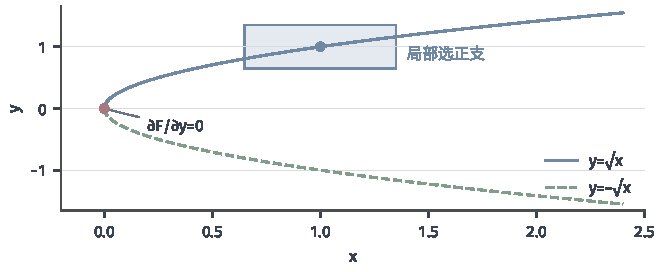
\includegraphics[width=112mm]{figures/01-mathematical-preliminaries-upper/01-mathematical-language-combinatorics-analysis-optimization/matplotlib/comprehension-additions/implicit-branches.pdf}
  \caption{方程$F(x,y)=y^2-x=0$的两支实数解。浅蓝矩形围住$(1,1)$，在该矩形内每个允许的$x$只有正支解，且$F_y=2y\neq0$；红点处$F_y=0$，两支相交。图的两个根都属于同一方程，选定起始解与邻域才确定隐函数分支。}
  \label{fig:vol1-add-implicit-branches}
\end{figure}
\FloatBarrier


\subsubsection{隐函数的存在、唯一性与微分}

下面的充分条件先保证局部解存在且唯一，再保证解随参数连续可微。
可逆性只要求待解变量对应的方阵Jacobian可逆，并非要求整个带参数映射为方阵。
\begin{theorem}[隐函数定理]
\label{thm:analysis-implicit-function}
设$F:\mathbb{R}^p\times\mathbb{R}^m\to\mathbb{R}^m$在 $(\bm{a},\bm{b})$的某个开邻域内连续可微， $F(\bm{a},\bm{b})=\bm{0}$，并且关于待解变量的Jacobian矩阵 \[   \bm{D}_{\bm{y}}F(\bm{a},\bm{b})   \in\mathbb{R}^{m\times m} \]
可逆。则存在$\bm{a}$与$\bm{b}$的邻域$U,V$，以及唯一的连续可微函数
$\varphi:U\to V$，使$\varphi(\bm{a})=\bm{b}$，并且对所有
$(\bm{x},\bm{y})\in U\times V$都有
\[
  F(\bm{x},\bm{y})=\bm{0}
  \quad\Longleftrightarrow\quad
  \bm{y}=\varphi(\bm{x}).
\]
其Jacobian矩阵满足
\begin{equation}
  \bm{D}\varphi(\bm{x})
  =
  -
  \bigl[\bm{D}_{\bm{y}}F(\bm{x},\varphi(\bm{x}))\bigr]^{-1}
  \bm{D}_{\bm{x}}F(\bm{x},\varphi(\bm{x})).
\label{eq:analysis-implicit-derivative}
\end{equation}
\end{theorem}

证明将方程改写为局部压缩迭代，再分别检查统一压缩、自映射与解的可微性；形式求导不能替代这些存在性步骤。
\begin{proof}
为证明定理~\ref{thm:analysis-implicit-function}的存在性，先把方程改写为局部压缩迭代。记
\[   \bm{A}   =   \bm{D}_{\bm{y}}F(\bm{a},\bm{b}),   \qquad   T_{\bm{x}}(\bm{y})   =   \bm{y}-\bm{A}^{-1}F(\bm{x},\bm{y}). \]
$F(\bm{x},\bm{y})=\bm{0}$当且仅当$T_{\bm{x}}(\bm{y})=\bm{y}$，即$\bm y$是更新后保持不变的点，称为不动点。并且
\[   \bm{D}_{\bm{y}}T_{\bm{x}}(\bm{y})   =   \bm{I}   -   \bm{A}^{-1}\bm{D}_{\bm{y}}F(\bm{x},\bm{y}), \]
它在$(\bm{a},\bm{b})$处为零。由导数连续性，可以选择闭球 $B=\{\bm{y}:\lVert\bm{y}-\bm{b}\rVert_2\leq r\}$和$\bm{a}$的邻域$U$，使
\begin{equation}
  \sup_{\bm{x}\in U,\,\bm{y}\in B}
  \left\lVert
    \bm{D}_{\bm{y}}T_{\bm{x}}(\bm{y})
  \right\rVert_{\mathrm{op}}
  \leq q<1.
\label{eq:analysis-ift-uniform-contraction}
\end{equation}
沿$\bm{y}$方向使用式~\eqref{eq:analysis-operator-mean-value-bound}可知，每个
$T_{\bm{x}}$都把$B$内任意两点之间的距离缩小到原来的至多$q$倍。

还必须核对自映射。因为$T_{\bm{a}}(\bm{b})=\bm{b}$且$T_{\bm{x}}(\bm{b})$关于 $\bm{x}$连续，可进一步缩小$U$，使
\[   \lVert T_{\bm{x}}(\bm{b})-\bm{b}\rVert_2   \leq\frac{1-q}{2}r. \]
于是对$\bm{y}\in B$，
\[
  \lVert T_{\bm{x}}(\bm{y})-\bm{b}\rVert_2
  \leq
  q\lVert\bm{y}-\bm{b}\rVert_2+\frac{1-q}{2}r
  \leq
  \frac{1+q}{2}r
  <r.
\]
所以$T_{\bm{x}}(B)$包含在$B$的内部$V$中。
固定$\bm x\in U$，从$\bm y_0=\bm b$出发，令$\bm y_{n+1}=T_{\bm x}(\bm y_n)$。
所有迭代项都留在$B$内，相邻差满足
$\lVert\bm y_{n+1}-\bm y_n\rVert_2\leq q^n\lVert\bm y_1-\bm y_0\rVert_2$。
增大$q$仍保留这个上界，因而可设$0<q<1$。对$m>n$，几何和给出
\[
 \lVert\bm y_m-\bm y_n\rVert_2
 \leq\sum_{j=n}^{m-1}\lVert\bm y_{j+1}-\bm y_j\rVert_2
 \leq\frac{q^n}{1-q}\lVert\bm y_1-\bm y_0\rVert_2\longrightarrow0.
\]
每个坐标都是实柯西列，所以该序列在有限维欧氏空间中收敛；闭性使极限仍在$B$内。
$T_{\bm x}$连续，令$n\to\infty$可得极限$\varphi(\bm x)$满足
$T_{\bm x}(\varphi(\bm x))=\varphi(\bm x)$，而映射的内部包含关系使它属于$V$。
若另有不动点$\bm z$，则
$\lVert\bm z-\varphi(\bm x)\rVert_2\leq q\lVert\bm z-\varphi(\bm x)\rVert_2$，
由$q<1$只能有$\bm z=\varphi(\bm x)$，所以这个不动点唯一。若
$(\bm{x},\bm{y})\in U\times V$且$F(\bm{x},\bm{y})=\bm{0}$，则$\bm{y}\in B$也是
$T_{\bm{x}}$的不动点，唯一性迫使$\bm{y}=\varphi(\bm{x})$。这证明了定理所述的局部
存在与零点集合的逐点唯一性。

还需说明所得解随参数连续可微。把$U$进一步缩小为开球，并使
$\overline U\times B$包含在原定义域内；这个集合闭且有界，关于$\bm x$的导数各分量连续，
故有统一范数上界$L$。对$\bm x,\bm x'\in U$，
两点间的线段仍在$U$内，式~\eqref{eq:analysis-operator-mean-value-bound}
可用于$T_{\bm x}(\bm y)$的参数变化。利用两个不动点关系，
\[   \lVert\varphi(\bm{x})-\varphi(\bm{x}')\rVert_2   \leq   q\lVert\varphi(\bm{x})-\varphi(\bm{x}')\rVert_2   +L\lVert\bm{x}-\bm{x}'\rVert_2, \]
移项得到$\lVert\varphi(\bm x)-\varphi(\bm x')\rVert_2
\leq L\lVert\bm x-\bm x'\rVert_2/(1-q)$，
故$\varphi$局部Lipschitz连续。令 $\bm{h}\to\bm{0}$并记 $\bm{k}=\varphi(\bm{x}+\bm{h})-\varphi(\bm{x})$，前述界给出 $\lVert\bm{k}\rVert_2=O(\lVert\bm{h}\rVert_2)$。对恒等式
\[   F(\bm{x}+\bm{h},\varphi(\bm{x})+\bm{k})   -   F(\bm{x},\varphi(\bm{x}))   =   \bm{0} \]
作一阶展开，得到
\[   \bm{D}_{\bm{x}}F\,\bm{h}   +   \bm{D}_{\bm{y}}F\,\bm{k}   +   o(\lVert\bm{h}\rVert_2)   =   \bm{0}. \]
展开中的Jacobian均在$(\bm x,\varphi(\bm x))$处取值，联合扰动的余项
$o(\lVert(\bm h,\bm k)\rVert_2)$因$\lVert\bm k\rVert_2=O(\lVert\bm h\rVert_2)$
成为$o(\lVert\bm h\rVert_2)$。
基点的$\det\bm A\neq0$，行列式又是矩阵元素的连续函数，
所以邻域足够小时$\bm D_{\bm y}F$仍可逆。于是
\[   \bm{k}   =   -   (\bm{D}_{\bm{y}}F)^{-1}   \bm{D}_{\bm{x}}F\,\bm{h}   +   o(\lVert\bm{h}\rVert_2). \]
这证明$\varphi$可微并给出式~\eqref{eq:analysis-implicit-derivative}；各Jacobian矩阵连续又保证$\bm{D}\varphi$连续。至此，隐函数定理中的存在、局部唯一与导数公式都已得到说明。证明中特别核对了自映射和统一压缩条件，只有形式上的固定点改写并不足够。
\end{proof}

\paragraph{隐函数的导数}

定理的证明已同时建立解分支的存在、唯一性、可微性及式~\eqref{eq:analysis-implicit-derivative}。计算时只需在选定分支上代入两个Jacobian；下面用最初的方程核对正、负分支各自的变化率。

\begin{example}[隐函数分支的导数]
设$F(x,y)=y^2-x$，在$(1,1)$处有$F=0$、$F_y=2\neq0$。
隐函数定理保证$(1,1)$附近的解可以唯一写成$y=\varphi(x)$，且
\[
 \varphi'(x)=-\frac{F_x(x,\varphi(x))}{F_y(x,\varphi(x))}
 =\frac1{2\varphi(x)},\qquad \varphi'(1)=\frac12.
\]
直接选正支$\varphi(x)=\sqrt x$，求导同样得到$1/(2\sqrt x)$。
若在$(1,-1)$附近选负支，导数则为$-1/2$；起始解不同，所追踪的函数也不同。
\end{example}


\subsubsection{反函数的存在与微分}

反求一个向量值映射的输入，可以看成以输出为参数的一组方程，从而回用隐函数的结论。
以下只保证邻域之间的逆，不预先断言整个定义域上的映射单射。
\begin{theorem}[局部反函数定理]
\label{thm:multivariable-inverse-function}
设$U\subseteq\mathbb R^d$开，$G:U\to\mathbb R^d$连续可微，$\bm a\in U$，且$\bm J_G(\bm a)$可逆。
则存在$\bm a$的开邻域$U_0$与$G(\bm a)$的开邻域$V_0$，使$G:U_0\to V_0$为双射，逆映射连续可微，并满足
\[
 \bm J_{G^{-1}}(G(\bm x))=[\bm J_G(\bm x)]^{-1}
 \qquad(\bm x\in U_0).
\]
\end{theorem}
\begin{proof}
以输出$\bm y$为参数、原输入$\bm x$为待解变量，令$H(\bm y,\bm x)=G(\bm x)-\bm y$。
在$(G(\bm a),\bm a)$处，关于$\bm x$的Jacobian就是可逆的$\bm J_G(\bm a)$。隐函数定理给出开邻域$V_0$、$W$以及$C^1$映射$\varphi:V_0\to W$，使
\[
 G(\bm x)=\bm y\quad\Longleftrightarrow\quad\bm x=\varphi(\bm y)
 \qquad(\bm y\in V_0,\ \bm x\in W).
\]
将$W$缩小并重新选取$V_0$，可使$W\subset U$且$\bm J_G$在$W$内均可逆。
令$U_0=W\cap G^{-1}(V_0)$，它因$G$连续而为包含$\bm a$的开集。
每个$\bm y\in V_0$都有$G(\varphi(\bm y))=\bm y$，故$\varphi(\bm y)\in U_0$；反之，每个$\bm x\in U_0$都由上述唯一性满足$\varphi(G(\bm x))=\bm x$。
因此$G:U_0\to V_0$为双射，逆就是$C^1$映射$\varphi$。
对$G(\varphi(\bm y))=\bm y$使用链式法则，得到$\bm J_G(\varphi(\bm y))\bm J_\varphi(\bm y)=\bm I$，左乘逆矩阵便得到所述公式。
\end{proof}

\paragraph{局部可逆与整体单射}

Jacobian处处可逆仍不保证整个定义域上单射。例如
$g(u,v)=(e^u\cos v,e^u\sin v)^\top$的Jacobian行列式为$e^{2u}>0$，
但$v$与$v+2\pi$给出同一输出。它在每一点附近可以反求，整个平面上的输入却会重复覆盖输出。
反过来，存在连续逆也不保证逆可微：一元函数$x\mapsto x^3$全局单射，
其逆在$0$处没有有限导数。使用局部逆定理时，需要逐项检查邻域、可微性和可逆Jacobian。

\FloatBarrier

\section{区域积分}
\label{sec:multivariable-region-integration}

一块不均匀的金属薄片占据平面区域$D$，在点$(x,y)$附近每单位面积的质量为$\rho(x,y)$。
把$D$切成许多小块，每块的质量约等于块内某一点的密度乘这块的面积；把所有小块的质量相加，就得到总质量的近似值，小块切得越细，近似越准确。
空间物体的质量、带电体的总电荷也按同样方式累计，只是面积换成体积，面密度换成体密度或电荷密度。
这类问题中的被积函数都是多元标量函数$f:D\subseteq\mathbb R^d\to\mathbb R$：输入是一个位置的$d$个坐标，输出是该位置上一个待累计的数。

同一个积分还有两种常用读法。
若$f\geq0$定义在平面区域$D$上，积分等于以$D$为底、以$f$的图像为顶的立体的体积，这是一元积分“曲线下方面积”在高一维的对应。
把积分除以$D$的面积，所得的数是$f$在$D$上的平均值，例如一个地区的平均降雨量或一块薄板的平均温度。

第~\ref{sec:analysis-measurability-integration}节在实轴上用长度给小块赋权，再由简单函数逼近和绝对可积要求建立了勒贝格积分。
推广到$\mathbb R^d$时只需更换两样东西：小块的大小改用$d$维体积来度量，函数的输入改为$\mathbb R^d$中的点。
简单函数逼近、单调收敛和支配收敛的论证只用到“分层、相加、取极限”，不依赖输入有几个坐标，可以原样沿用。

定义建立以后，还要回答计算上的三个问题。
第一，能否先算每一条切片上的累计，再把各切片的结果累加，也就是把区域积分拆成逐个坐标的一元积分？答案取决于非负性或绝对可积性，它们保证两种累计次序给出同一个区域积分。
第二，圆盘、球体等区域在直角坐标下边界复杂，能否改用极坐标、球坐标描述？换坐标会放大或缩小每个小块的体积，需要用Jacobian行列式校正。
第三，被积函数依赖一个参数时，积分值怎样随参数变化，能否在积分号下求导？
本节先建立多维测度与区域积分，再依次讨论这三个问题。切片与坐标计算的更多例题可参考\scite{math-openstax-calculus3}。

\subsection{多维测度与乘积测度}
\label{sec:comb-multidimensional-product-measure}

区域积分首先要回答“一块区域有多大”。
实轴上的长度已经由勒贝格测度给出；平面上的面积、空间中的体积也需要同样精确的定义，否则无法给边界弯曲、带有无穷多个小洞或形状不规则的区域赋予大小。
本小节先把第~\ref{sec:comb-set-measurement}节的区间覆盖构造搬到$\mathbb R^d$，再说明把$\mathbb R^d$拆成$\mathbb R^p\times\mathbb R^q$（$d=p+q$）时，$d$维体积怎样由$p$维与$q$维的体积相乘得到。
后一点是第~\ref{sec:multivariable-iterated-integrals}节累次积分成立的测度基础。

\subsubsection{多维勒贝格测度}

\paragraph{坐标盒}

实轴上的构造从区间出发，因为区间的长度不需要另行定义。
$\mathbb R^d$中与区间对应的对象是各坐标方向上区间的笛卡尔积，称为坐标盒，例如
\[
 Q=\prod_{i=1}^d(a_i,b_i),\qquad a_i<b_i.
\]
平面上的坐标盒是各边平行于坐标轴的长方形，空间中的坐标盒是长方体。
坐标盒的体积规定为各边长之积$\operatorname{vol}(Q)=\prod_i(b_i-a_i)$，例如$(0,2)\times(0,3)$的面积为$6$。
这条规定推广了长方形面积公式，也与有限集合的计数规则$|A\times B|=|A||B|$一致：一个方向排$m$个单位格、另一个方向排$n$个单位格时，共有$mn$个单位格。
闭盒、半开盒与同端点开盒的体积相同；某一边长为零的退化盒，例如平面上的一条线段，体积为零。

\paragraph{多维勒贝格测度}

一维外测度用可数个区间覆盖集合，再取覆盖总长度的下确界。
把区间换成开坐标盒、把长度换成体积，就得到$\mathbb R^d$上的外测度
\[
 m_d^*(E)=\inf_{\substack{E\subseteq\bigcup_{n=1}^{\infty}Q_n\\
 Q_n\text{为开坐标盒}}}\sum_{n=1}^{\infty}\operatorname{vol}(Q_n),
\]
其中下确界取遍$E$的所有可数开盒覆盖。
直观上，这是用盒子从外侧包住$E$，看至少需要多少总体积。

按这个定义，线段和可数点集的面积都是零。
线段$[0,1]\times\{0\}$能被一个开盒$(-\varepsilon,1+\varepsilon)\times(-\varepsilon,\varepsilon)$覆盖，这个盒的面积$2\varepsilon(1+2\varepsilon)$可以任意小，所以线段的二维外测度为零：线段有长度，却没有面积。
把$\mathbb Q^2$的点排成一列，第$k$个点放进面积为$\varepsilon2^{-k}$的小盒，这些小盒的总面积不超过$\varepsilon$，因此$\mathbb Q^2$的二维外测度也为零，论证与实轴上可数集零测相同。

可测集仍沿用定义~\ref{def:analysis-lebesgue-measurable-set}的分割要求：若集合$A\subseteq\mathbb R^d$对每个测试集合$E\subseteq\mathbb R^d$满足
$m_d^*(E)=m_d^*(E\cap A)+m_d^*(E\setminus A)$，就称$A$为$d$维勒贝格可测集。
一维情形中关于外测度的可数次可加性、可测集族构成$\sigma$代数、测度的可数可加性以及零测集子集可测的论证，只用到覆盖、取下确界和分割这几种操作，没有用到区间只有一个方向，所以把区间换成盒以后可以逐步照搬。
于是$d$维勒贝格可测集组成$\sigma$代数$\mathcal L(\mathbb R^d)$；把$m_d^*$限制在$\mathcal L(\mathbb R^d)$上，得到$d$维勒贝格测度$m_d$，其中$m_1$就是第~\ref{sec:comb-set-measurement}节的$m$。
$m_d$是完备的，即零测集的子集都可测。
需要另作核对的只有$m_d(Q)=\operatorname{vol}(Q)$，即可数个盒的覆盖不会把一个盒的体积算小；它对应一维中“区间的外测度等于其长度”的论证，这里不再重复。

常用的集合都在这个可测范围内。
坐标半空间$\{\bm x:x_i\leq t\}$的可测性与一维半直线相同：把每个覆盖盒沿超平面$x_i=t$切成两块，两块的体积之和仍是原盒的体积；坐标盒由这类半空间经取补集和可数次交、并得到，因而也可测。
每个欧氏开集又都是其中有理端点开盒的可数并：对开集中的每一点，先取一个包含该点且完全落在开集内的开盒，再把端点向内调整为有理数，使盒仍包含该点；有理端点的盒只有可数个。
因此$\mathcal L(\mathbb R^d)$包含全部开集，从而包含由全部开集（等价地，由全部开盒）生成的Borel $\sigma$代数$\mathcal B(\mathbb R^d)$；由于$m_d$完备，勒贝格范围还包含Borel零测集的全部子集。

\paragraph{平移与伸缩}

把集合$E$平移一个向量$\bm a$，每个覆盖盒也随之平移，盒的边长不变，所以$m_d(E+\bm a)=m_d(E)$。
把集合按比例$c>0$伸缩为$cE=\{c\bm x:\bm x\in E\}$时，每个覆盖盒的每条边都乘$c$，体积乘$c^d$，而$E$的覆盖与$cE$的覆盖一一对应，因此
\[
 m_d(cE)=c^dm_d(E).
\]
这正是“长度按$c$倍、面积按$c^2$倍、体积按$c^3$倍变化”的精确形式。
例如平面圆环$\{1\leq\lVert\bm x\rVert_2<2\}$放大$2^k$倍后得到$\{2^k\leq\lVert\bm x\rVert_2<2^{k+1}\}$，面积变为原来的$4^k$倍；示例~\ref{ex:region-power-function-threshold}判别幂函数的可积性时会用到这个事实。
一般线性映射对体积的放大倍数是行列式的绝对值，留到第~\ref{sec:multivariable-change-variables}节讨论。

\subsubsection{乘积测度}

累次积分要把$\mathbb R^d$看成$\mathbb R^p\times\mathbb R^q$，先在$\mathbb R^q$方向累计，再在$\mathbb R^p$方向累计。
为此需要知道$d$维体积与$p$维、$q$维体积之间的关系。
对坐标盒，答案已经包含在定义里：$d$条边长之积等于前$p$条边长之积乘后$q$条边长之积。
还需要确认两件事：对一般的Borel集合$A\subseteq\mathbb R^p$与$B\subseteq\mathbb R^q$，乘积集合$A\times B$（下文称为矩形）的体积是否仍为$m_p(A)m_q(B)$；只规定矩形的体积，能否唯一确定其余集合的$d$维体积。

\paragraph{矩形赋值的乘法规则}

矩形上的乘法规则可以先在只有有限个格子的情形中看清。
\begin{example}[有限网格上的乘积权重]
\label{ex:region-finite-product-weights}
横向分为两列，权重（可以理解为两段的长度或两组点的总质量）分别为$1,2$；纵向分为两行，权重分别为$3,4$。
规定每个格子的联合权重等于所在列、行权重之积，四个格子的权重就是$1\cdot3=3$、$2\cdot3=6$、$1\cdot4=4$、$2\cdot4=8$。
逐格相加得到总量
\[
 3+6+4+8=21=(1+2)(3+4),
\]
右侧先把两侧权重各自相加再相乘，两侧相等正是有限分配律。
先求每一行的总量$3+6=9$、$4+8=12$再相加，或先求每一列的总量$3+4=7$、$6+8=14$再相加，也都得到$21$。
\end{example}

逐格、逐行、逐列三种求和次序给出同一个总量，这就是累次积分在有限情形中的样子。
图~\ref{fig:analysis-process-product-measure-grid}把列宽和行高分别按两侧权重画成比例，格子面积因而等于乘积权重。
乘法规则只描述一种特定的联合赋权方式，一般的二元分布不必由两侧权重相乘得到。

\begin{figure}[!htbp]
 \centering
 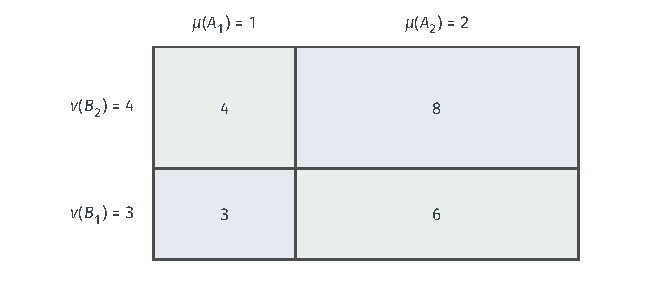
\includegraphics[width=112mm]{figures/01-mathematical-preliminaries-upper/00-shared/tikz/chapter3-concept-processes/product-measure-grid.pdf}
 \caption{两列的权重分别为$1,2$（图中记为$\mu(A_1),\mu(A_2)$），两行的权重分别为$3,4$（记为$\nu(B_1),\nu(B_2)$）。四个格子的乘积权重为$3,6,4,8$，总量$21=(1+2)(3+4)$。列宽与行高按各自权重成比例，因此格子面积也按乘积成比例。这只是乘积赋权的有限示例，并非任意二维分布都满足的关系。}
 \label{fig:analysis-process-product-measure-grid}
\end{figure}

\paragraph{乘积$\sigma$代数}

矩形适合规定基本赋值，但矩形的并或补一般不再是矩形，例如两个长方形拼成的L形区域就不是矩形，因此不能只把矩形本身当作全部可测集合。
设$A\in\mathcal B(\mathbb R^p)$、$B\in\mathcal B(\mathbb R^q)$，称$A\times B$为Borel矩形。
包含全部Borel矩形的最小$\sigma$代数称为乘积$\sigma$代数，记为$\mathcal B(\mathbb R^p)\otimes\mathcal B(\mathbb R^q)$。
它和直接在$\mathbb R^{p+q}$中由开盒生成的Borel范围是同一个集合族：
\begin{equation}
 \mathcal B(\mathbb R^p)\otimes\mathcal B(\mathbb R^q)=\mathcal B(\mathbb R^{p+q}).
 \label{eq:comb-borel-product-structure}
\end{equation}

先证右侧包含于左侧。$\mathbb R^{p+q}$中的每个开盒都是$\mathbb R^p$中一个开盒与$\mathbb R^q$中一个开盒的乘积，因而是Borel矩形；每个开集又是可数个开盒的并，所以全部开集都在左侧，左侧作为$\sigma$代数就包含它们生成的$\mathcal B(\mathbb R^{p+q})$。

再证左侧包含于右侧，只需说明每个Borel矩形都是$\mathbb R^{p+q}$中的Borel集合。
考虑所有满足$A\times\mathbb R^q\in\mathcal B(\mathbb R^{p+q})$的集合$A\subseteq\mathbb R^p$。
开盒$A$使$A\times\mathbb R^q$成为开集，所以开盒都满足要求；又因为$(\mathbb R^p\setminus A)\times\mathbb R^q$是$A\times\mathbb R^q$的补集、$\bigl(\bigcup_nA_n\bigr)\times\mathbb R^q=\bigcup_n(A_n\times\mathbb R^q)$，满足要求的集合对补集和可数并封闭。
这些集合因而构成一个包含开盒的$\sigma$代数，从而包含全部$\mathcal B(\mathbb R^p)$。
同理$\mathbb R^p\times B$对每个$B\in\mathcal B(\mathbb R^q)$都是Borel集合，于是
$A\times B=(A\times\mathbb R^q)\cap(\mathbb R^p\times B)$属于$\mathcal B(\mathbb R^{p+q})$。
左侧的生成集合都在右侧，所以左侧包含于右侧。

\paragraph{乘积测度}

有了可测范围，还要为其中每个集合赋予联合的大小。对Borel矩形，所需规则就是把两个方向的测度相乘。

\begin{definition}[乘积测度]
\label{def:analysis-product-measure}
设$p,q\geq1$。在$\mathcal B(\mathbb R^p)\otimes\mathcal B(\mathbb R^q)$上，若一个测度对所有$A\in\mathcal B(\mathbb R^p)$、$B\in\mathcal B(\mathbb R^q)$满足
\begin{equation}
 (m_p\otimes m_q)(A\times B)=m_p(A)m_q(B),
 \label{eq:comb-product-measure-rectangle}
\end{equation}
就称它为$m_p$与$m_q$的\term{乘积测度}（product measure），记为$m_p\otimes m_q$，其中约定$0\cdot\infty=0$。
\end{definition}

约定$0\cdot\infty=0$有直观依据：平面上的直线$\mathbb R\times\{0\}$在横向长度无穷、纵向长度为零，它应当没有面积。
定义只规定了矩形应有的测度，还要确认这个规定能够一致地扩展到整个乘积$\sigma$代数，并且扩展只有一种。

\begin{theorem}[乘积测度的存在唯一性]
在$\mathcal B(\mathbb R^p)\otimes\mathcal B(\mathbb R^q)$上恰有一个测度满足式~\eqref{eq:comb-product-measure-rectangle}，它就是$m_{p+q}$在$\mathcal B(\mathbb R^{p+q})$上的限制。
\end{theorem}

存在性由$m_{p+q}$本身提供：对坐标盒，矩形规则就是体积的定义；从盒推进到一般Borel矩形，要利用两侧Borel集合都能被可数个盒从外侧逼近，这一步引用测度论教材\scite{math-folland1999real}。
唯一性的论证依赖两点：两个矩形的交仍是矩形；$\mathbb R^{p+q}$能被可数个有限体积的盒$(-n,n)^{p+q}$逐步填满。
两个测度若在全部矩形上取值相同，先在每个有限体积的盒内比较，再令$n\to\infty$，就能推出它们在整个乘积$\sigma$代数上相同，完整论证见同一教材。
两个一般测度空间也可以按同样的矩形规则作乘积，那时“能被可数个有限测度部分填满”成为必须单独检查的条件；一般的构造与条件见第~\ref{chap:measure-spaces}章。

\paragraph{欧氏乘积与完备化}

上面的乘积测度只定义在Borel范围上，而区域积分使用的是更大的勒贝格范围$\mathcal L(\mathbb R^{p+q})$。
两者之间相差的只是零测集的子集：每个勒贝格可测集都能写成一个Borel集合与某个Borel零测集的子集之并\scite{math-folland1999real}。
把这些零测集的子集也补进可测范围，称为完备化；$m_{p+q}$在$\mathcal L(\mathbb R^{p+q})$上正是$m_p\otimes m_q$的完备化。

完备化不能靠先把两个因子完备化来代替：即使两个因子都取完备的勒贝格测度，它们的乘积$\sigma$代数也未必完备。
\begin{example}[勒贝格因子的乘积$\sigma$代数不完备]
\label{ex:region-product-sigma-algebra-incomplete}
取$p=q=1$，考虑由全部乘积$A\times B$（$A,B\in\mathcal L(\mathbb R)$）生成的乘积$\sigma$代数$\mathcal L(\mathbb R)\otimes\mathcal L(\mathbb R)$。

先说明其中每个集合$E$在每个$x$处的截面$E_x=\{y:(x,y)\in E\}$都勒贝格可测。
截面都可测的集合组成的族包含全部乘积$A\times B$，因为$(A\times B)_x$是$B$或$\varnothing$。取截面与取补集、可数并可以交换次序：$(\mathbb R^2\setminus E)_x=\mathbb R\setminus E_x$，$\bigl(\bigcup_nE_n\bigr)_x=\bigcup_n(E_n)_x$；所以这个族是$\sigma$代数，从而包含整个乘积$\sigma$代数。

再取一个勒贝格不可测集$S\subseteq\mathbb R$（第~\ref{sec:comb-set-measurement}节指出这类集合存在），令$E=\{0\}\times S$。
$E$包含在直线$\{0\}\times\mathbb R$中。这条直线是乘积$\{0\}\times\mathbb R$，乘积测度给它的值为$m(\{0\})m(\mathbb R)=0\cdot\infty=0$，所以$E$是乘积测度下零测集的子集；在完备的勒贝格范围$\mathcal L(\mathbb R^2)$中，$E$可测且零测。
但$E$在$x=0$处的截面是不可测集$S$，所以$E$不属于乘积$\sigma$代数。
\end{example}

因此下面陈述累次积分时，要分清函数对Borel范围可测，还是只对勒贝格范围可测；后者的结论需要附加“几乎处处”。

\subsection{区域积分的定义与可积性}
\label{sec:multivariable-riemann-lebesgue}

测度确定区域有多大，被积函数确定各位置贡献多少。
现在把一元可测函数与勒贝格积分的定义搬到$\mathbb R^d$上：改变的是输入空间和所用的测度，积分的构造步骤不变。

\subsubsection{多元可测函数}

累计函数值时，要把输入按函数值分层，例如取值在$[u,v)$之间的位置组成一层，这一层的贡献约为函数值乘该层的体积。
只有每一层都能测量，这种累计才有意义。
与一元情形一样，只需检查所有阈值集合$\{f>a\}$，因为$\{f\geq u\}=\bigcap_n\{f>u-1/n\}$、$\{u\leq f<v\}=\{f\geq u\}\setminus\{f\geq v\}$等集合都能由阈值集合经可数次集合运算得到。
\begin{definition}[多元可测函数]
设$D\in\mathcal L(\mathbb R^d)$。函数$f:D\to\overline{\mathbb R}$称为勒贝格可测函数，是指对每个$a\in\mathbb R$，集合
\[
 \{\bm x\in D:f(\bm x)>a\}
\]
都属于$\mathcal L(\mathbb R^d)$。若这些集合都属于$\mathcal B(\mathbb R^d)$，则称$f$为Borel可测函数。
\end{definition}

连续函数都可测：若$f$在$D$上连续，阈值集合$\{f>a\}$是开区间$(a,\infty)$的原像，因而相对于$D$开，可写为$D$与某个欧氏开集之交；$D$与开集都可测，所以阈值集合可测。
连续性只是可测性的充分条件：$\mathbb I_{\mathbb Q^d}$处处不连续，却是可测函数，因为它的阈值集合在$a<0$、$0\leq a<1$、$a\geq1$时分别是全空间、$\mathbb Q^d$和$\varnothing$，而可数集$\mathbb Q^d$零测，因而可测。

第~\ref{sec:analysis-measurable-functions}节关于和、积、绝对值、最大最小值以及逐点极限保持可测性的论证只用到阈值集合的可数运算，在$\mathbb R^d$上照样成立。
例如分段给出的函数$f=g\mathbb I_{D_1}+h\mathbb I_{D_2}$，只要$g,h$在$\mathbb R^d$上连续、$D_1,D_2$可测，就是可测函数。
向量值函数的积分按分量进行，每个分量都是本节讨论的标量函数；例如质心的每个坐标都是一个标量区域积分与总质量之比。

\subsubsection{区域积分的定义}

\paragraph{非负标量函数的积分}

先累计非负贡献，就不会遇到正负无穷相消。
可测简单函数在每个可测小块上取常值，其积分等于各块的常值乘该块测度再求和；一般非负函数仍由下方的简单函数逼近。
\begin{definition}[区域上非负可测函数的积分]
设$D\in\mathcal L(\mathbb R^d)$，$f:D\to[0,\infty]$可测。定义
\[
 \int_D f\,\mathrm dm_d
 =\sup_{\substack{0\leq s\leq f\\s\text{为可测简单函数}}}
 \int_D s\,\mathrm dm_d.
\]
若$s=\sum_{j=1}^n c_j\mathbb I_{E_j}$，其中$E_j\subseteq D$可测、两两不交且$c_j\geq0$，则$\int_Ds\,\mathrm dm_d=\sum_jc_jm_d(E_j)$，约定$0\cdot\infty=0$。
\end{definition}

把$f$看成薄片的面密度，就能读出这个定义的含义。
满足$0\leq s\leq f$的简单函数把区域分成有限块，并在每块上用一个不超过真实密度的常数代替密度，所以$\int_Ds$是总质量的一个偏小估计；对所有这样的估计取上确界，就得到总质量。

也可以从体积来读：$c_j\mathbb I_{E_j}$对应以$E_j$为底、高为$c_j$的柱体$E_j\times[0,c_j)$，由乘积测度的矩形规则，它的$(d+1)$维体积就是$c_jm_d(E_j)$。
于是$\int_Ds$是排在$f$的图像下方的一组柱体的总体积，上确界则是图像下方整个区域的体积；第~\ref{sec:multivariable-iterated-integrals}节会用Tonelli定理把这个读法写成等式。

这个积分可以取$+\infty$，例如$f\equiv1$在整个平面上的积分是平面的面积$+\infty$。
在全空间上把$f$作零延拓，就有
$\int_Df\,\mathrm dm_d=\int_{\mathbb R^d}f\mathbb I_D\,\mathrm dm_d$，其中$f\mathbb I_D$在$D$内等于$f$、在$D$外取零；以后在区域上积分，都可以看成对零延拓后的函数在全空间上积分。
区域不必是矩形，定义也不要求它的边界零测；这与黎曼积分先用矩形网格逼近区域的做法不同。

\paragraph{有符号标量函数的积分}

函数可以取正负值时，例如带电薄片上既有正电荷也有负电荷，应先分别累计正负贡献：$f^+=\max\{f,0\}$给出正电荷的密度，$f^-=\max\{-f,0\}$给出负电荷的密度，净电荷是两者总量之差。
与一元情形相同，为了让这个差是一个普通的有限数，要求绝对值的总贡献有限。
\begin{definition}[区域上可测函数的积分]
设$D\in\mathcal L(\mathbb R^d)$，$f:D\to\overline{\mathbb R}$可测。若
\begin{equation}
 \int_D|f|\,\mathrm dm_d<\infty,
 \label{eq:multivariable-lebesgue-integrability}
\end{equation}
称$f$在$D$上勒贝格可积，并定义
\[
 \int_Df\,\mathrm dm_d=\int_Df^+\,\mathrm dm_d-\int_Df^-\,\mathrm dm_d.
\]
\end{definition}

由于$|f|=f^++f^-$，条件~\eqref{eq:multivariable-lebesgue-integrability}同时保证正负两部分的积分都有限，相减不会出现$\infty-\infty$。
这个条件不成立时，至少有一部分积分为无穷；若两部分都为无穷，两者之差没有意义，也就不能用相减定义勒贝格积分。

条件~\eqref{eq:multivariable-lebesgue-integrability}还保证$f$几乎处处取有限值。
集合$N=\{|f|=\infty\}$对每个$M>0$满足$M\mathbb I_N\leq|f|$，所以$Mm_d(N)\leq\int_D|f|$对所有$M$成立，只能$m_d(N)=0$；在$N$上把无穷值改成零，不改变积分。

与黎曼积分相比，这一定义不要求函数在细小的网格块上接近常数。
例如$\mathbb I_{\mathbb Q^d}$在单位立方体上不黎曼可积：每个小盒中都既有有理点又有无理点，上和恒为$1$而下和恒为$0$；但它的勒贝格积分为零，因为可数集的$d$维测度为零。

\paragraph{二重积分与多重积分}

二维时把上述积分写为
\[
 \iint_Df(x,y)\,\mathrm dx\,\mathrm dy=\int_Df\,\mathrm dm_2;
\]
三维中常记为$\iiint_Df\,\mathrm dV$；$d$维时统一写作
\[
 \int_Df(\bm x)\,\mathrm d\bm x=\int_Df\,\mathrm dm_d.
\]
“二重”或“多重”表示输入维数，并不表示已经选择了逐坐标的计算次序。
例如$f\equiv3$、$D=[0,1]\times[0,2]$时，积分为$3m_2(D)=6$：密度处处为$3$、面积为$2$的薄片，总质量为$6$。

当$0<m_d(D)<\infty$且$f$可积时，
\[
 \frac{1}{m_d(D)}\int_Df\,\mathrm dm_d
\]
称为$f$在$D$上的平均值。
它是一个常数，用它代替$f$铺满整个$D$，总累计不变。上例的平均值为$3$。

\subsubsection{可积性的判别}

按定义，可测函数$f$在$D$上可积，意思是非负积分$\int_D|f|\,\mathrm dm_d$有限。
这个非负积分总有定义，只是可能等于$+\infty$；判别可积性因此只需回答一个问题：$|f|$在$D$上的总累计是有限还是无穷。
直接从上确界定义计算这个量往往不现实，下面三种做法都用更容易得到的量来估计它：用函数的上界乘区域的测度；用一列测度有限的递增子区域逼近$D$，看这些子区域上的累计是否有共同上界；与一个已知是否可积的函数逐点比较。

若$f$有界且$D$的测度有限，第一种做法立即给出有限上界。
由此可见，累计变为无穷只能是因为$f$无界（例如在某些位置附近无界），或者$D$的测度无穷；后两种做法正是为这两种情形准备的。

\paragraph{有界函数且有界区域}

设区域$D$有界，从而$m_d(D)<\infty$（更一般地，只要$m_d(D)<\infty$即可），$f$可测且$|f|\leq M<\infty$几乎处处成立。
这时$|f|\leq M\mathbb I_D$几乎处处成立，由非负积分的单调性，
\[
 \int_D|f|\,\mathrm dm_d\leq M m_d(D)<\infty.
\]
物理上，总质量不超过最大密度乘面积。
由定理~\ref{thm:multivariable-extreme-value}，闭有界集上的连续函数有界，所以闭有界区域上的连续函数可积。

这一判别只用到有界性，不要求函数能连续地延伸到区域的边界。
\begin{example}[开正方形上剧烈振荡的有界函数可积]
\label{ex:region-bounded-oscillation}
在开正方形$(0,1)^2$上令$f(x,y)=\sin\bigl(1/(xy)\bigr)$。
$f$在开正方形上连续，因而可测。
它不能连续延拓到闭正方形：固定$x=t\in(0,1)$，令$y\downarrow0$，则$1/(ty)\to+\infty$，$f(t,y)$在$-1$与$1$之间无穷次振荡，没有极限。
所以闭有界集上的极值定理不能直接使用。
但$|f|\leq1$且$m_2\bigl((0,1)^2\bigr)=1$，由上面的估计，
\[
 \int_{(0,1)^2}|f|\,\mathrm dm_2\leq1,
\]
所以$f$在$(0,1)^2$上可积。
\end{example}

这个判别不适用于两类情形：函数无界，或区域的测度无穷。
在这两类情形中，可积与不可积都可能发生。
无界函数仍可能可积，示例~\ref{ex:region-power-function-threshold}将说明$\lVert\bm x\rVert_2^{-1}$在平面单位圆盘上可积；无限测度区域上的有界函数则未必可积，例如$f\equiv1$在整个平面上积分为无穷。
判断这两类情形需要更细的估计。

\paragraph{无界函数或无限区域}

处理无界函数或无限区域时，可以先避开麻烦的位置。
取一列递增的可测集合$D_1\subseteq D_2\subseteq\cdots$，使$\bigcup_nD_n=D$，并让每个$D_n$避开函数无界的位置、只占有限测度；例如函数只在原点附近无界时，可取$D_n=D\cap\{1/n\leq\lVert\bm x\rVert_2\leq n\}$。
这时每个$\int_{D_n}|f|$通常可以用有界函数在有限测度区域上的估计确认有限。
由于$0\leq|f|\mathbb I_{D_n}\uparrow|f|\mathbb I_D$，单调收敛定理（定理~\ref{thm:analysis-monotone-convergence}）给出
\[
 \int_D|f|\,\mathrm dm_d
 =\lim_{n\to\infty}\int_{D_n}|f|\,\mathrm dm_d
 =\sup_n\int_{D_n}|f|\,\mathrm dm_d.
\]
因此$f$在$D$上可积，当且仅当截断累计$\int_{D_n}|f|$有一个与$n$无关的有限上界。
这就是定理~\ref{thm:analysis-improper-nonnegative-criterion}在$\mathbb R^d$中的形式，证明只用单调收敛，不依赖维数。
只知道每个截断累计分别有限还不够，必须检查它们是否共同有界。

截断累计也可以改写成级数。
把区域拆成两两不交的“壳层”$A_k=D_k\setminus D_{k-1}$（$D_0=\varnothing$），由积分的区域可加性（定理~\ref{thm:analysis-integral-set-additivity}），
$\int_D|f|=\sum_k\int_{A_k}|f|$，可积性就化为一个非负级数是否收敛。

只依赖半径的函数适合用壳层估计。
下面按半径成倍增长划分壳层，判别平面幂函数在原点附近和远处的可积性。
\begin{example}[平面幂函数$\lVert\bm x\rVert_2^{-p}$的可积阈值]
\label{ex:region-power-function-threshold}
设$p>0$，$f(\bm x)=\lVert\bm x\rVert_2^{-p}$，$\bm x\in\mathbb R^2\setminus\{\bm 0\}$。按半径成倍增长的圆环
\[
 A_k=\{\bm x\in\mathbb R^2:2^k\leq\lVert\bm x\rVert_2<2^{k+1}\},\qquad k\in\mathbb Z
\]
把$\mathbb R^2\setminus\{\bm 0\}$分成两两不交的壳层。

记$\alpha=m_2(A_0)$。它是一个有限正数：$A_0$含有小盒，又含于盒$(-2,2)^2$。
由伸缩性质，$A_k=2^kA_0$，所以$m_2(A_k)=4^k\alpha$。
在$A_k$上$2^{-(k+1)p}<\lVert\bm x\rVert_2^{-p}\leq2^{-kp}$，乘以$m_2(A_k)$得到
\[
 2^{-p}\alpha\,2^{k(2-p)}\leq\int_{A_k}\lVert\bm x\rVert_2^{-p}\,\mathrm d\bm x\leq\alpha\,2^{k(2-p)}.
\]

单位圆外由$k=0,1,2,\ldots$的壳层组成，各壳层的贡献与公比为$2^{2-p}$的几何级数同阶，累计有限当且仅当$p>2$。
单位圆内（去掉原点）由$k=-1,-2,\ldots$的壳层组成；令$j=-k$，各壳层的贡献与$2^{j(p-2)}$同阶，累计有限当且仅当$p<2$。
因此$\lVert\bm x\rVert_2^{-p}$在单位圆盘上可积当且仅当$p<2$，在单位圆外可积当且仅当$p>2$；$p=2$时两侧都不可积，在整个平面上则对任何$p>0$都不可积。
\end{example}

在$\mathbb R^d$中把面积因子$4^k$换成$2^{kd}$，同样的计算给出阈值$d$；$d=1$就是第~\ref{sec:analysis-improper-integrals}节的阈值$1$。
这个阈值比较的是两种速度：靠近原点时，函数按$r^{-p}$增大，而半径约为$r$的壳层的体积按$r^d$缩小；远离原点时，函数按$r^{-p}$减小，壳层的体积按$r^d$增大。
第~\ref{sec:multivariable-change-variables}节将用极坐标直接计算圆环上的积分，验证这里的结论（示例~\ref{ex:region-polar-power-check}）。

确认可积以后，截断积分还能用来计算有符号积分。
由$|f\mathbb I_{D_n}|\leq|f|$，支配收敛定理（定理~\ref{thm:analysis-dominated-convergence}）给出$\int_{D_n}f\to\int_Df$，误差不超过$\int_{D\setminus D_n}|f|$，所以无论选哪一列递增区域，都得到同一个值。

缺少绝对可积性时，截断极限可能依赖区域的选法。
\begin{example}[截断极限依赖截断方式]
\label{ex:region-truncation-dependence}
在平面上令$f(x,y)=1$（$x>0$），$f(x,y)=-1$（$x\leq0$）。
取正方形$D_n=(-n,n)^2$时，右半部分与左半部分的面积都是$2n^2$，正负贡献恰好抵消，每个$\int_{D_n}f=0$。
取偏向右侧的长方形$D_n'=(-n,2n)\times(-n,n)$时，右侧部分面积为$4n^2$，左侧部分面积为$2n^2$，所以$\int_{D_n'}f=2n^2\to+\infty$。
两列截断都递增地填满整个平面，极限却分别是$0$和$+\infty$。
\end{example}

例中$\int|f|=+\infty$，两种截断的不同极限都不能当作$f$的积分。
截断只能用来计算已经确认绝对可积的函数的积分。

\paragraph{比较判别：可积上界与不可积下界}

有了一族可积性已知的函数，就可以把新函数与它们逐点比较，而不必每次重新做壳层计算。
比较有两个方向，都来自非负积分的单调性：
\begin{itemize}
 \item 若存在非负可积函数$H$，使$|f|\leq H$在$D$上几乎处处成立，则$\int_D|f|\leq\int_DH<\infty$，$f$可积；
 \item 若存在非负可测函数$g$，使$|f|\geq g$在$D$上几乎处处成立且$\int_Dg=+\infty$，则$\int_D|f|=+\infty$，$f$不可积。
\end{itemize}
比较只需在可能出问题的位置进行：先用区域可加性把$D$拆成函数有界且测度有限的部分和“原点附近”“远处”等部分，前者用有界判别，其余部分再与幂函数比较。

远处的比较看函数衰减得有多快。
\begin{example}[远处与$r^{-3}$和$r^{-2}$比较]
\label{ex:region-comparison-at-infinity}
记$r=\lVert\bm x\rVert_2$，其中$\bm x=(x,y)$。

函数$f(x,y)=\cos(xy)/(1+x^2+y^2)^{3/2}$在整个平面上可积。
在单位圆盘内$|f|\leq1$，用有界判别；在单位圆外$|f|\leq(1+r^2)^{-3/2}\leq r^{-3}$，而由示例~\ref{ex:region-power-function-threshold}，$p=3>2$的幂函数在圆外可积。

函数$g(x,y)=1/(1+x^2+y^2)$在整个平面上不可积。
在单位圆外$1+r^2\leq2r^2$，所以$g\geq r^{-2}/2$，而$p=2$的幂函数在圆外累计无穷。
\end{example}

一元的$1/(1+x^2)$在实轴上可积，二元的类似函数却不可积。
原因在于远处可用的范围增长得更快：半径为$R$的圆盘面积按$R^2$增长，而区间$[-R,R]$的长度只按$R$增长。

原点附近的比较同样只看奇点处的增长速度。
\begin{example}[原点附近的对数奇点与平方倒数奇点]
\label{ex:region-comparison-near-origin}
仍记$r=\lVert\bm x\rVert_2$，在单位圆盘$\{r\leq1\}$上考察两个在原点附近无界的函数。

$\log(x^2+y^2)=2\log r$在$r\downarrow0$时趋于$-\infty$。
函数$t\mapsto t|\log t|$在$(0,1)$上的最大值为$1/e$，在$t=1/e$处取到，所以$0<r<1$时
\[
 |\log r^2|=2|\log r|\leq\frac2e\,r^{-1}.
\]
与$p=1<2$的幂函数比较，可知$\log(x^2+y^2)$在单位圆盘上可积。

$(x^2+2y^2)^{-1}$满足$x^2+2y^2\leq2(x^2+y^2)=2r^2$，所以$(x^2+2y^2)^{-1}\geq r^{-2}/2$。
与$p=2$的幂函数比较，可知它在单位圆盘上不可积。
\end{example}

找不到合适的比较函数时，还可以用第~\ref{sec:multivariable-iterated-integrals}节的Tonelli定理把$\int_D|f|$化为累次积分直接计算，再判断它是否有限。

\subsection{区域积分的基本性质}

多维区域积分仍是按第~\ref{sec:analysis-measurability-integration}节方式构造的勒贝格积分，只是测度换成了$m_d$。
那里的单调收敛定理、Fatou引理、支配收敛定理以及下面各条积分性质，证明都只用到简单函数逼近、测度的可数可加性和这些结论之间的推导，不依赖输入只有一个坐标，因此在$\mathbb R^d$上可以直接使用。
下面固定可测区域$D$，各有符号公式均要求所列函数在相应区域上绝对可积，微元统一写为$\mathrm dm_d$。

\paragraph{加法}

若$f,g$在$D$上可积，则$f+g$也可积，且
\[
 \int_D(f+g)\,\mathrm dm_d=\int_Df\,\mathrm dm_d+\int_Dg\,\mathrm dm_d.
\]
绝对可积性由$|f+g|\leq|f|+|g|$保证，相加公式由一般勒贝格积分的线性给出。
物理上，两种物质叠放在同一块薄片上时，总质量等于两种物质的质量之和。

\paragraph{减法}

若$f,g$在$D$上可积，则
\[
 \int_D(f-g)\,\mathrm dm_d=\int_Df\,\mathrm dm_d-\int_Dg\,\mathrm dm_d.
\]
这里两项都是有限数，因此不会出现无穷减无穷。

\paragraph{数乘}

若$c\in\mathbb R$且$f$在$D$上可积，则$cf$可积，并满足
\[
 \int_Dcf\,\mathrm dm_d=c\int_Df\,\mathrm dm_d.
\]
系数只改变各位置的标量贡献，不改变积分区域及其测度；例如把密度的单位从千克换成克，总质量的数值同样乘$1000$。

\paragraph{区域可加性}

若$f$在有限个或可数个两两不交的可测集合$D_j$之并上可积，则
\[
 \int_{\bigcup_jD_j}f\,\mathrm dm_d=\sum_j\int_{D_j}f\,\mathrm dm_d.
\]
也就是说，把一块区域分成若干块分别累计再相加，与整体累计相同。
有限并直接来自指示函数的分解，可数并使用一般积分的区域可加性；绝对可积性保证右侧级数绝对收敛。

两块区域允许重叠时，只需扣除被重复计入的交集：
\[
 \int_{A\cup B}f\,\mathrm dm_d
 =\int_Af\,\mathrm dm_d+\int_Bf\,\mathrm dm_d-\int_{A\cap B}f\,\mathrm dm_d.
\]
这由$\mathbb I_{A\cup B}=\mathbb I_A+\mathbb I_B-\mathbb I_{A\cap B}$得到。
若沿连续函数的图像这类曲线或曲面把区域切成几块，公共边界是零测集（第~\ref{sec:multivariable-iterated-integrals}节用Tonelli定理证明这一点），重叠部分不影响积分，因此可以直接把各块的积分相加。

\paragraph{单调性}

若$f,g$在$D$上可积且$f\leq g$几乎处处成立，则
\[
 \int_Df\,\mathrm dm_d\leq\int_Dg\,\mathrm dm_d.
\]
特别地，$a\leq f\leq b$几乎处处成立且$0<m_d(D)<\infty$时，有$a\,m_d(D)\leq\int_Df\leq b\,m_d(D)$，即平均值落在$[a,b]$内。
同一估计也给出忽略一小块区域$E$时的误差上界：若在$E$上$|f|\leq M$，则舍去$E$造成的误差$\bigl|\int_Ef\bigr|$不超过$Mm_d(E)$。

\paragraph{绝对值不等式}

可积函数满足
\[
 \left|\int_Df\,\mathrm dm_d\right|\leq\int_D|f|\,\mathrm dm_d.
\]
它来自$-|f|\leq f\leq|f|$和积分单调性。左侧允许正负贡献相消，右侧不允许，因此净量的大小不超过总量。

由于零测集贡献为零，上述所有性质都允许在零测集上修改有限函数值；测度的完备性保证这种修改保持可测。

\subsection{累次积分}
\label{sec:multivariable-iterated-integrals}

直接从定义计算区域积分往往不现实。
求一块面包的体积时，可以先把它切成平行的薄片，每片的体积约为截面面积乘片厚，再把所有薄片的体积相加。
同样，求薄片的总质量时，可以先沿每一条竖线累计质量，得到这条竖线上的“线密度”，再沿横向累计各条竖线的贡献。
这种“先在每个截面上累计，再累计截面”的计算称为累次积分，它把一次$d$维累计化成几次低维累计。
累次积分是否等于区域积分，要检查非负性或绝对可积性；交换累计次序也不只是调换微分记号的位置。

\subsubsection{截面与累次积分}

把$\mathbb R^d$写成$\mathbb R^p\times\mathbb R^q$，点写成$(\bm x,\bm y)$，其中$\bm x\in\mathbb R^p$、$\bm y\in\mathbb R^q$；最常见的是$p=q=1$。
对$f:\mathbb R^p\times\mathbb R^q\to\overline{\mathbb R}$，固定$\bm x$所得的函数$f_{\bm x}(\bm y)=f(\bm x,\bm y)$称为关于$\bm y$的截面。
区域$D$上的函数先作零延拓，截面就在$D$的截面$D_{\bm x}=\{\bm y:(\bm x,\bm y)\in D\}$以外取零；例如单位圆盘在$x\in[-1,1]$处的截面是区间$[-\sqrt{1-x^2},\sqrt{1-x^2}]$。

若各截面的积分有意义，所得关于$\bm x$的函数的积分也有意义，则
\[
 \int_{\mathbb R^p}\left(\int_{\mathbb R^q}f(\bm x,\bm y)\,\mathrm d\bm y\right)\mathrm d\bm x
\]
称为先对$\bm y$、再对$\bm x$的累次积分。
内层积分把$\bm x$视为固定的数，算出截面$D_{\bm x}$上的总量；外层积分再把这些截面总量按$\bm x$累计。
交换两组变量的角色，就得到先对$\bm x$、再对$\bm y$的累次积分。
两种次序是否相等，以及它们是否等于区域积分，不能由记号推出，要由下面的定理判断。

有限网格上的这种计算就是先求每行的加权和，再把各行的结果相加；示例~\ref{ex:region-finite-product-weights}和图~\ref{fig:analysis-process-product-measure-grid}中两种次序都得到$21$。
那里的联合权重是两侧权重之积；二元概率分布何时能写成两个边缘分布的乘积，即独立性问题，可参考\BookChapterRef{chap:probability-theory}{卷2《数学准备：概率、因果与决策》的“随机变量与概率基础”章}。

\subsubsection{累次积分的成立条件}

下面先对Borel可测函数陈述结论，这时每个截面都Borel可测。
若函数只对勒贝格范围$\mathcal L(\mathbb R^{p+q})$可测，就可能出现示例~\ref{ex:region-product-sigma-algebra-incomplete}中的现象：该例中集合$E$的指示函数勒贝格可测，却在零面积的直线$x=0$上取不可测的截面。
因此对勒贝格可测函数，截面的可测性和内层积分都只对几乎每个坐标成立。

\paragraph{非负可测函数的累次积分}

非负贡献不会因相消而改变总量，因此允许总积分为无穷。
Tonelli定理说明，对非负函数，两种次序的累次积分都等于区域积分。
\begin{theorem}[Tonelli定理]
\label{thm:analysis-tonelli-fubini}
设$p,q\geq1$，$f:\mathbb R^p\times\mathbb R^q\to[0,\infty]$为Borel可测函数。则每个截面$\bm y\mapsto f(\bm x,\bm y)$与$\bm x\mapsto f(\bm x,\bm y)$都Borel可测，两个内层积分函数
\[
 \bm x\longmapsto\int_{\mathbb R^q}f(\bm x,\bm y)\,\mathrm d\bm y,\qquad
 \bm y\longmapsto\int_{\mathbb R^p}f(\bm x,\bm y)\,\mathrm d\bm x
\]
也分别Borel可测，且
\[
 \begin{aligned}
 \int_{\mathbb R^{p+q}}f\,\mathrm dm_{p+q}
 &=\int_{\mathbb R^p}\left(\int_{\mathbb R^q}f(\bm x,\bm y)\,\mathrm d\bm y\right)\mathrm d\bm x\\
 &=\int_{\mathbb R^q}\left(\int_{\mathbb R^p}f(\bm x,\bm y)\,\mathrm d\bm x\right)\mathrm d\bm y.
 \end{aligned}
\]
三个积分允许共同取$+\infty$。若$f$只是勒贝格可测，上述等式仍成立，但截面只对几乎每个$\bm x$（相应地，几乎每个$\bm y$）勒贝格可测，内层积分函数只在几乎处处有定义，且是勒贝格可测函数。
\end{theorem}

\paragraph{绝对可积函数的累次积分}

有符号函数不能只依靠逐行或逐列的有限值来保证换序。
先对$|f|$应用非负版本，确认整个区域上的绝对贡献有限，就能排除正负无穷相消。
\begin{theorem}[Fubini定理]
\label{thm:analysis-fubini-integrable}
设$f:\mathbb R^p\times\mathbb R^q\to\overline{\mathbb R}$勒贝格可测，并满足
$\int_{\mathbb R^{p+q}}|f|\,\mathrm dm_{p+q}<\infty$。
则截面$f_{\bm x}$对几乎每个$\bm x$可积，另一方向的截面也对几乎每个$\bm y$可积。
把内层积分函数在相应例外集上置为零后，它们分别可积，并且
\[
 \begin{aligned}
 \int_{\mathbb R^{p+q}}f\,\mathrm dm_{p+q}
 &=\int_{\mathbb R^p}\left(\int_{\mathbb R^q}f(\bm x,\bm y)\,\mathrm d\bm y\right)\mathrm d\bm x\\
 &=\int_{\mathbb R^q}\left(\int_{\mathbb R^p}f(\bm x,\bm y)\,\mathrm d\bm x\right)\mathrm d\bm y.
 \end{aligned}
\]
三个积分都是有限值。若$f$是Borel可测函数，例外集以外的截面也都是Borel可测函数。
\end{theorem}

若$f$在零测集上取无穷值，可先把那些值改成零再处理有符号积分；定义有符号积分时已经说明，绝对积分有限时这个集合零测，改值不影响积分。

两个定理的证明可分为集合与函数两层，这里只给出依赖路线，不把矩形上的核对当作完整证明。
集合层从矩形出发。
对矩形指示函数$\mathbb I_{A\times B}$，固定$\bm x$后的内层积分是$\mathbb I_A(\bm x)m_q(B)$，外层积分是$m_p(A)m_q(B)$，由乘积测度的矩形规则，它也等于$m_{p+q}(A\times B)$；有限可加性把这个结论推广到有限个不交矩形之并。
从这些集合推进到乘积$\sigma$代数中的任意Borel集合，需要测度论的扩张论证，不是仅靠每个矩形上的等式便能完成，完整论证见\scite{math-folland1999real}。

函数层沿用积分的构造步骤。
集合层的结论就是指示函数的结论，经线性组合推广到非负简单函数，再取简单函数列$s_n\uparrow f$，由单调收敛推广到任意非负Borel可测函数，得到Tonelli定理。
对勒贝格可测函数，先找一个与它几乎处处相等的Borel可测函数，二者的差异包含在一个Borel零测集$N$中；对$\mathbb I_N$用Tonelli定理得$\int m_q(N_{\bm x})\,\mathrm d\bm x=m_{p+q}(N)=0$，所以几乎每个截面$N_{\bm x}$零测，修改不影响内层积分。
若$f$绝对可积，则对$f^+$和$f^-$分别应用Tonelli定理；绝对积分有限保证两部分不会出现无穷减无穷，相减即得Fubini定理。
对两个更一般的测度作乘积时，Tonelli与Fubini定理在相应的有限覆盖条件下同样成立，见第~\ref{chap:measure-spaces}章。

两个定理合起来给出一个实用的判别。
先对$|f|$应用Tonelli定理：只要任意一种次序的非负累次积分$\int\left(\int|f|\,\mathrm d\bm y\right)\mathrm d\bm x$有限，区域绝对积分就有限；随后才能对$f$使用Fubini定理，在两种次序之间自由切换。

Tonelli定理也把“积分等于图像下方的体积”写成了等式。
设$f:\mathbb R^d\to[0,\infty]$为Borel可测函数，令$\Gamma=\{(\bm x,t)\in\mathbb R^d\times\mathbb R:0\leq t<f(\bm x)\}$为图像下方的区域。
若$0\leq t<f(\bm x)$，就能取有理数$r$使$t<r<f(\bm x)$，所以
$\Gamma=\bigcup_{r\in\mathbb Q,\,r>0}\bigl(\{f>r\}\times[0,r)\bigr)$是可数个Borel矩形之并，是Borel集合。
对$\mathbb I_\Gamma$先沿$t$方向积分，固定$\bm x$时的截面是区间$[0,f(\bm x))$，长度为$f(\bm x)$，于是
\[
 m_{d+1}(\Gamma)=\int_{\mathbb R^d}\left(\int_{\mathbb R}\mathbb I_\Gamma(\bm x,t)\,\mathrm dt\right)\mathrm d\bm x=\int_{\mathbb R^d}f\,\mathrm dm_d.
\]

同样的截面论证说明图像本身没有体积。
设$f$是有限值Borel函数，它的图像$\{(\bm x,f(\bm x))\}$是Borel函数$(\bm x,t)\mapsto t-f(\bm x)$的零点集，因而是Borel集合；图像在每个$\bm x$处的截面只有一个点，长度为零，由Tonelli定理，图像是$(d+1)$维零测集。
例如圆周由上下两个半圆的图像组成，因此面积为零；把区域沿这类曲线切开时，边界确实不影响积分。

\subsubsection{累次积分的计算}

设$R=[a,b]\times[c,d]$，其中$a<b$、$c<d$，且$f$在$R$上连续。
连续函数在闭有界矩形上有界，因而在$R$上绝对可积，Fubini定理保证可以先按一个坐标累计、再按另一个坐标累计，且两种次序给出同一结果：
\[
 \begin{aligned}
 \int_R f(x,y)\,\mathrm d(x,y)
 &=\int_a^b\left(\int_c^d f(x,y)\,\mathrm dy\right)\mathrm dx\\
 &=\int_c^d\left(\int_a^b f(x,y)\,\mathrm dx\right)\mathrm dy.
 \end{aligned}
\]
左侧是一次区域累计，右侧两个累次积分是具体的逐次计算；三者相等依赖Fubini定理的条件。

计算内层积分时，另一个坐标当作常数。
\begin{example}[矩形上$x+y$的两种累次积分]
\label{ex:region-rectangle-iterated}
令$f(x,y)=x+y$，$R=[0,1]\times[0,2]$，$f$在$R$上连续。先对$y$积分，
\[
 \int_0^1\left[xy+\frac{y^2}{2}\right]_{y=0}^{y=2}\,\mathrm dx
 =\int_0^1(2x+2)\,\mathrm dx=3.
\]
内层运算把$x$视为固定数，结果$2x+2$是竖线$\{x\}\times[0,2]$上的累计，再交给外层积分。
先对$x$积分，则
\[
 \int_0^2\left[\frac{x^2}{2}+xy\right]_{x=0}^{x=1}\,\mathrm dy
 =\int_0^2\left(\frac12+y\right)\mathrm dy=3,
\]
两种次序给出同一结果。区域面积为$2$，所以$f$在$R$上的平均值为$3/2$。
\end{example}

一般区域先作零延拓。
若区域写为$D=\{(x,y):a\leq x\leq b,\ \alpha(x)\leq y\leq\beta(x)\}$，其中上下边界$\alpha\leq\beta$在$[a,b]$上连续，则$D$是闭集，固定$x$的截面是区间$[\alpha(x),\beta(x)]$。
因此对$D$上非负可测或可积的$f$，有
\[
 \iint_Df\,\mathrm dx\,\mathrm dy=\int_a^b\left(\int_{\alpha(x)}^{\beta(x)}f(x,y)\,\mathrm dy\right)\mathrm dx.
\]
内积分的上下限$\alpha(x),\beta(x)$正是截面的两个端点。改变积分次序时，应改为固定$y$、重新描述同一个区域的横截面。

同一个区域可以有两种截面描述，换序时两套上下限都要从区域本身读出。
\begin{example}[三角形区域上交换积分次序]
\label{ex:region-triangle-order-swap}
令$D=\{(x,y):0\leq y\leq x\leq1\}$，在$D$上累计常数$1$。
固定$x\in[0,1]$时，纵截面是$0\leq y\leq x$，先对$y$积分得到
\[
 \int_0^1\left(\int_0^x1\,\mathrm dy\right)\mathrm dx=\int_0^1x\,\mathrm dx=\frac12.
\]
固定$y\in[0,1]$时，同一区域的横截面是$y\leq x\leq1$，先对$x$积分得到
\[
 \int_0^1\left(\int_y^11\,\mathrm dx\right)\mathrm dy=\int_0^1(1-y)\,\mathrm dy=\frac12.
\]
两种次序都给出三角形的面积$1/2$。
\end{example}

若只交换微分记号而保留原来的上下限，所描述的就不再是同一个区域。
图~\ref{fig:analysis-process-region-slicing-orders}把这两种切片画在同一个区域上，突出换序时内层上下限也要改变。
\begin{figure*}[!htbp]
 \centering
 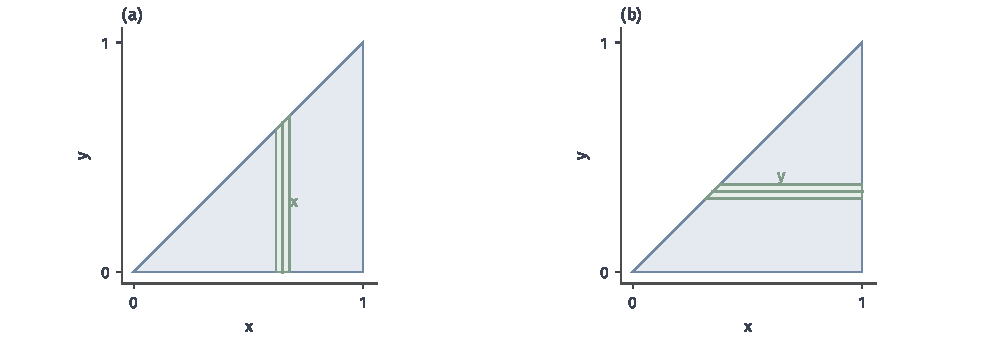
\includegraphics[width=169.0mm]{figures/01-mathematical-preliminaries-upper/00-shared/matplotlib/chapter3-concept-processes/region-slicing-orders.pdf}
 \caption{$D=\{0\leq y\leq x\leq1\}$在两图完全相同。(a) 固定$x$，纵截面为$0\leq y\leq x$；(b) 固定$y$，横截面为$y\leq x\leq1$。绿色窄条仅示意一次切片，图中的条宽不充当实际微元。两种累计$1$都得面积$1/2$；换序依据非负性或绝对可积性，而非图形本身。}
 \label{fig:analysis-process-region-slicing-orders}
\end{figure*}

换序有时决定一个积分能否算出来。
\begin{example}[换序计算含$e^{y^2}$的累次积分]
\label{ex:region-exp-square-order-swap}
考虑
\[
 \int_0^1\left(\int_x^1e^{y^2}\,\mathrm dy\right)\mathrm dx.
\]
内层的$e^{y^2}$没有初等原函数，按原次序无法用原函数直接计算。
积分区域是闭三角形$\{(x,y):0\leq x\leq y\leq1\}$，被积函数在其上连续，因而绝对可积，可以交换次序。
固定$y\in[0,1]$时，横截面是$0\leq x\leq y$，于是
\[
 \int_0^1\left(\int_0^ye^{y^2}\,\mathrm dx\right)\mathrm dy
 =\int_0^1ye^{y^2}\,\mathrm dy
 =\frac{e-1}{2}.
\]
\end{example}

内层对$x$积分时$e^{y^2}$是常数，只产生截面长度$y$，而这个因子$y$恰好使外层积分有原函数$\frac12e^{y^2}$。

\subsubsection{积分换序的适用边界}

非负函数没有正负相消，累计可以为无穷；绝对可积函数允许取正负值，但正负两部分的累计各自有限。
两者都缺失时，两种累计次序可能以不同方式配对正负贡献，交换次序就可能改变结果，甚至一个次序收敛而另一个次序发散。

最直观的例子来自双重级数。
设$a_{i,j}$（$i,j\geq1$）是一个无穷矩阵，在第一象限上令
$f(x,y)=a_{i,j}$于$(x,y)\in[i-1,i)\times[j-1,j)$，即每个边长为$1$的方格上取对应的矩阵元素。
对$x\in[i-1,i)$，截面积分$\int_0^\infty f(x,y)\,\mathrm dy=\sum_ja_{i,j}$是第$i$行的和（在各项非负或该行绝对收敛时）；再对$x$积分，就得到“先行后列”的累次和$\sum_i\sum_ja_{i,j}$。
另一种次序同理给出$\sum_j\sum_ia_{i,j}$，而$\int|f|\,\mathrm dm_2=\sum_{i,j}|a_{i,j}|$。

因此，Tonelli定理说明非负双重级数可以任意交换求和次序，Fubini定理说明绝对收敛的双重级数也可以这样做。
缺少绝对收敛时，即使每一行、每一列的和都有限，两种次序也可能给出不同的结果。

\begin{example}[行列各自可加仍不足以换序]
\label{ex:analysis-iterated-sum-failure}
令$a_{i,j}=\mathbb I\{j=i\}-\mathbb I\{j=i+1\}$（$i,j\geq1$），并按上面的方格构造第一象限上的阶梯函数$f$。
每一行只有一个$1$和一个$-1$，故$\sum_j a_{i,j}=0$；
第一列只有$a_{1,1}=1$，和为$1$；第$j\geq2$列有$a_{j,j}=1$与$a_{j-1,j}=-1$，和为$0$。于是
\[
 \sum_{i=1}^{\infty}\left(\sum_{j=1}^{\infty}a_{i,j}\right)=0,
 \qquad
 \sum_{j=1}^{\infty}\left(\sum_{i=1}^{\infty}a_{i,j}\right)=1,
\]
即$f$的两种累次积分分别为$0$和$1$。
两种累次积分都有有限值，却不相等。每行的绝对值和为$2$，所以$\int|f|\,\mathrm dm_2=+\infty$，
正负部分也各为无穷。失效的是Fubini定理的绝对可积条件，而非某一行的计算规则。
\end{example}

图~\ref{fig:vol1-add-fubini-cancellation-grid}显示这个例子的两条对角线。
逐行求和时，每个$+1$与同一行右侧的$-1$配对；逐列求和时，每个$-1$与同一列下方的$+1$配对，第一列的$+1$则没有配对对象。
由于绝对和无穷，Fubini定理不能保证这两种配对给出同一结果。
\begin{figure}[!htb]
  \centering
  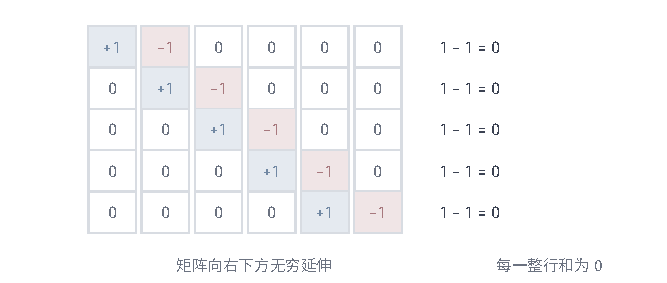
\includegraphics[width=112mm]{figures/01-mathematical-preliminaries-upper/00-shared/tikz/mathematical-language-combinatorics-analysis-optimization-comprehension-additions/fubini-cancellation-grid.pdf}
  \caption{无穷矩阵$a_{i,j}=\mathbb I\{j=i\}-\mathbb I\{j=i+1\}$的左上角，展示前五行、前六列，矩阵向右下方继续；每个单元格也可看成第一象限中边长为$1$的方格。每一整行的和为$0$；第一整列的和为$1$，其他整列的和为$0$。蓝、红单元分别为$+1,-1$，每行绝对和为$2$，因而无穷矩阵不绝对可加。}
  \label{fig:vol1-add-fubini-cancellation-grid}
\end{figure}

连续函数也会出现同样的现象。
\begin{example}[$(x^2-y^2)/(x^2+y^2)^2$的两种累次积分不同]
\label{ex:region-rational-non-fubini}
在$(0,1)^2$上取
\[
 f(x,y)=\frac{x^2-y^2}{(x^2+y^2)^2}.
\]
直接求导可得$\partial_y\bigl(y/(x^2+y^2)\bigr)=f(x,y)$，所以固定$x>0$时
\[
 \int_0^1f(x,y)\,\mathrm dy=\left[\frac{y}{x^2+y^2}\right]_{y=0}^{y=1}=\frac{1}{1+x^2},
\]
再对$x$积分得到$\pi/4$。
由于$f(y,x)=-f(x,y)$，先对$x$积分时内层结果是$-1/(1+y^2)$，这一次序得到$-\pi/4$。

两个结果不同，原因仍是绝对可积性失效。
在$0<y<x$处$f>0$，所以
\[
 \int_0^1|f(x,y)|\,\mathrm dy\geq\int_0^xf(x,y)\,\mathrm dy=\left[\frac{y}{x^2+y^2}\right]_{y=0}^{y=x}=\frac{1}{2x},
\]
而$\int_0^11/(2x)\,\mathrm dx=+\infty$，由Tonelli定理，$\int_{(0,1)^2}|f|\,\mathrm dm_2=+\infty$。
\end{example}

在极坐标下$|f|=|\cos2\theta|/r^2$，这正是示例~\ref{ex:region-power-function-threshold}中$p=2$的临界幂次：原点附近正负两部分各自累计无穷。

\subsection{区域积分的换元}
\label{sec:multivariable-change-variables}

累次积分保留原坐标，只改变累计次序。
换元则用一个向量值映射$T$改变位置的坐标表示，例如用半径与角度描述圆盘中的点。
换坐标以后，函数要按新坐标重写，每个小块的体积也要重新计算：参数空间中大小相同的小块，映到原空间后可能大小不同。

\subsubsection{换元公式与适用条件}

\paragraph{体积的局部缩放}

一元换元$x=T(t)$中，参数的小区间$[t,t+\Delta t]$被映成长约$|T'(t)|\Delta t$的小区间，因子$|T'(t)|$记录长度的缩放（定理~\ref{thm:analysis-lebesgue-change-variables}）。
多元换元要把参数空间中的小块换成体积，先看线性映射。
方阵$\bm A$把单位正方体映成由$\bm A$的各列张成的平行多面体，其体积为$|\det\bm A|$；更一般地，对任意可测集合$E$都有$m_d(\bm AE)=|\det\bm A|\,m_d(E)$\scite{math-folland1999real}。

几个特例可以直接核对。
对角矩阵$\operatorname{diag}(a_1,\ldots,a_d)$分别伸缩各坐标，体积比例为$\prod_j|a_j|$，这正是坐标盒的体积规则。
正交矩阵（旋转与反射）保持距离，不改变图形的形状和大小，行列式为$\pm1$。
剪切矩阵$\begin{bmatrix}1&s\\0&1\end{bmatrix}$把正方形推成等底等高的平行四边形，面积不变，行列式也等于$1$。
公式取行列式的绝对值，是因为反射这类改变定向的映射行列式为负，而体积必须非负。

对可微的非线性映射$T$，由式~\eqref{eq:analysis-jacobian-linearization}，在一点$\bm x$附近有$T(\bm x+\bm h)\approx T(\bm x)+\bm J_T(\bm x)\bm h$。
于是以$\bm x$为角、边长为$\varepsilon$的小方块$Q$，被$T$映成一个近似的平行多面体，其体积约为$|\det\bm J_T(\bm x)|\varepsilon^d$；图~\ref{fig:analysis-process-jacobian-grid-cell}画出了这种小块的变化。

设$g$是原空间中的密度。用小方块$Q_k$铺满参数区域，记$\bm x_k$为$Q_k$的一个角，每块映成的小块$T(Q_k)$中的质量约为
\[
 g(T(\bm x_k))\,m_d(T(Q_k))\approx g(T(\bm x_k))|\det\bm J_T(\bm x_k)|\varepsilon^d.
\]
对$k$求和后，左侧的和近似原空间中的总质量，右侧的和近似参数空间中函数$g(T(\bm x))|\det\bm J_T(\bm x)|$的积分。
因此$g\circ T\,|\det\bm J_T|$是“每单位参数体积所含的质量”：它把原空间中按单位体积计的密度，换算成按参数小块计的密度。

这个局部说明还不是整个积分公式的证明。
整体上还必须控制每块的近似误差在加总以后趋于零，并且确保$T$把每个点只覆盖一次：若两个参数小块映到同一块正体积区域，那里的质量就会被计算两次。

\paragraph{勒贝格积分的换元}

开集之间的$C^1$微分同胚同时满足这两项要求：连续可微保证局部的体积规则，双射保证全局只覆盖一次。
定理直接对勒贝格可测函数陈述，连续被积函数是其特例。
\begin{theorem}[区域积分的换元公式]
设$U,V\subseteq\mathbb R^d$为开集，$T:U\to V$为$C^1$双射，逆映射也为$C^1$，且$\det\bm J_T$处处非零。
对任意非负勒贝格可测函数$g:V\to[0,\infty]$，有
\begin{equation}
 \int_Vg(\bm y)\,\mathrm d\bm y
 =\int_Ug(T(\bm x))|\det\bm J_T(\bm x)|\,\mathrm d\bm x,
 \label{eq:measurable-change-variables}
\end{equation}
允许共同值为$+\infty$。若$g$有符号且在$V$上绝对可积，则变换后的函数也绝对可积，等式仍成立并取有限值。
\end{theorem}

这类变换及其逆在定义域的每个闭有界子集上满足Lipschitz条件，因而把零测集映为零测集。
所以勒贝格可测函数$g$与$T$复合后仍勒贝格可测：Borel集合的原像仍是Borel集合，零测集的原像仍是零测集，而每个勒贝格可测集都是Borel集合与零测集子集之并。

一般定理先建立可测集合的体积变换$m_d(T(E))=\int_E|\det\bm J_T|$，再从指示函数进入简单函数，最后以单调逼近得到非负函数的公式；有符号情形对$|g|$、$g^+$和$g^-$分别应用非负结论即可。
这里说明的是证明的依赖关系，集合层的体积变换定理引用测度论教材\scite{math-folland1999real}，不把逐点线性化当作完整证明。

若只在可测子区域$D\subseteq U$上积分，对$V$中的函数$g\mathbb I_{T(D)}$应用同一公式，即得
\begin{equation}
 \int_{T(D)}g(\bm y)\,\mathrm d\bm y
 =\int_Dg(T(\bm x))|\det\bm J_T(\bm x)|\,\mathrm d\bm x.
 \label{eq:analysis-multivariate-change-variables}
\end{equation}
这里不另加有界或边界零测的要求；所需条件仍是非负可测，或者有符号且绝对可积。

常用坐标在原点、坐标轴或角度的接缝处不是微分同胚，例如极坐标在原点处所有角度都对应同一点。
若在参数区域和原区域中各去掉一个零测集以后，参数化成为开集之间的$C^1$微分同胚，就可以先在剩下的范围内换元，再补回零测集，因为零测集对积分没有贡献。
若参数化在正测度区域上重复覆盖，则不能直接使用这个单次覆盖版本。

\subsubsection{常用坐标变换}

\paragraph{极坐标}

圆盘的边界用直角坐标描述时，积分上下限会含平方根。
以半径$r$和角度$\theta$作为坐标，圆盘变成参数矩形$[0,1]\times[0,2\pi]$，但面积权重必须增加半径因子。
在平面上画出同心圆$r=$常数与射线$\theta=$常数组成的网格：介于$r$与$r+\Delta r$、$\theta$与$\theta+\Delta\theta$之间的小块，径向边长为$\Delta r$，弧向边长约为$r\Delta\theta$，所以面积约为$r\Delta r\Delta\theta$。
同样大小的参数块，离原点越远，对应的面积越大；靠近原点时则被压缩得很小。
这一面积权重正是极坐标映射的Jacobian行列式：示例~\ref{ex:multivariable-polar-jacobian}已算出$\det\bm J=r$。下面用它计算单位圆盘的面积，并检查换元公式的条件。
\begin{example}[用极坐标计算单位圆盘的面积]
\label{ex:analysis-polar-coordinate-jacobian}
令$D=\{\bm x\in\mathbb R^2:\lVert\bm x\rVert_2\leq1\}$，并令$T(r,\theta)=(r\cos\theta,r\sin\theta)$。
在开集$U=(0,1)\times(0,2\pi)$上，$T$是到$V$的$C^1$双射，逆映射也是$C^1$，其中$V$是开圆盘去掉线段$[0,1)\times\{0\}$（含原点）后的区域。
由示例~\ref{ex:multivariable-polar-jacobian}，$|\det\bm J_T(r,\theta)|=r$，在$U$上处处非零。
$D$与$V$只相差边界圆周和线段$[0,1)\times\{0\}$，它们都是零测集，因此
\[
 \int_D1\,\mathrm d\bm x
 =\int_V1\,\mathrm d\bm x
 =\int_0^{2\pi}\int_0^1r\,\mathrm dr\,\mathrm d\theta
 =\pi.
\]
最后一步在参数矩形上使用Tonelli定理，积分上下限包含端点不改变积分值。
若让$\theta$取遍$(0,4\pi)$，圆盘就会被覆盖两次，按公式算出的$2\pi$不再是面积，这正是单次覆盖条件排除的情形。
\end{example}

图~\ref{fig:vol1-add-polar-area-weight}说明半径因子来自哪里。同样的角度变化在较大半径处扫过更长的弧，故同样大小的参数块对应更大的面积，积分权重必须随半径变化。
\begin{figure}[!htb]
  \centering
  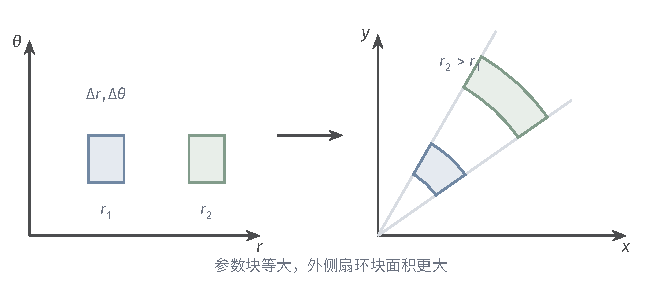
\includegraphics[width=112mm]{figures/01-mathematical-preliminaries-upper/00-shared/tikz/mathematical-language-combinatorics-analysis-optimization-comprehension-additions/polar-area-weight.pdf}
  \caption{极坐标映射中的两个等大参数块，具有相同的$\Delta r,\Delta\theta$，但外侧半径$r_2$较大。对应扇环块的精确面积为$(r\Delta r+(\Delta r)^2/2)\Delta\theta$，一阶项为$r\Delta r\Delta\theta$，因此面积元为$r\,\mathrm dr\,\mathrm d\theta$。图只比较局部块，坐标原点与接缝的处理见正文。}
  \label{fig:vol1-add-polar-area-weight}
\end{figure}

用极坐标可以直接核对示例~\ref{ex:region-power-function-threshold}得到的阈值。
\begin{example}[用极坐标核对幂函数的可积阈值]
\label{ex:region-polar-power-check}
设$0<a<b$，在圆环$\{a\leq\lVert\bm x\rVert_2\leq b\}$上积分$\lVert\bm x\rVert_2^{-p}$。
在开集$(a,b)\times(0,2\pi)$上使用极坐标，被去掉的两条圆周和一条线段都是零测集；被积函数只依赖半径，于是
\[
 \int_{a\leq\lVert\bm x\rVert_2\leq b}\lVert\bm x\rVert_2^{-p}\,\mathrm d\bm x
 =\int_0^{2\pi}\int_a^br^{-p}\cdot r\,\mathrm dr\,\mathrm d\theta
 =2\pi\int_a^br^{1-p}\,\mathrm dr.
\]
令$a\downarrow0$，它有界当且仅当$1-p>-1$，即$p<2$；令$b\to\infty$，它有界当且仅当$1-p<-1$，即$p>2$，与壳层估计一致。
取$p=0$、$a=1$、$b=2$，得到$2\pi\int_1^2r\,\mathrm dr=3\pi$，这就是示例~\ref{ex:region-power-function-threshold}中的$\alpha=m_2(A_0)$。
\end{example}

面积因子$r$正是壳层估计中“面积随半径增长”的来源：半径约为$r$、厚度为$\Delta r$的细圆环，面积约为$2\pi r\Delta r$。

极坐标与累次积分结合，还能计算一个没有初等原函数的一元积分。
\begin{example}[用极坐标计算Gauss积分]
\label{ex:region-gauss-integral}
函数$e^{-x^2}$没有初等原函数，但平面函数$e^{-(x^2+y^2)}$非负，在极坐标下只依赖半径。
对开集$(0,\infty)\times(0,2\pi)$使用换元公式，被去掉的原点和正$x$轴是零测集，于是
\[
 \int_{\mathbb R^2}e^{-(x^2+y^2)}\,\mathrm d(x,y)
 =\int_0^{2\pi}\int_0^\infty e^{-r^2}r\,\mathrm dr\,\mathrm d\theta
 =2\pi\cdot\frac12=\pi.
\]
另一方面，由Tonelli定理，左侧等于
\[
 \begin{aligned}
 \int_{\mathbb R}\left(\int_{\mathbb R}e^{-x^2}e^{-y^2}\,\mathrm dy\right)\mathrm dx
 &=\int_{\mathbb R}e^{-x^2}\,\mathrm dx\cdot\int_{\mathbb R}e^{-y^2}\,\mathrm dy\\
 &=\left(\int_{\mathbb R}e^{-x^2}\,\mathrm dx\right)^2.
 \end{aligned}
\]
这个积分为正，因此$\int_{\mathbb R}e^{-x^2}\,\mathrm dx=\sqrt\pi$。
\end{example}

这个结果给出正态分布密度的归一化常数。
计算同时用到了换元和累次积分：换元把平面积分变成可算的径向积分，累次积分把同一个平面积分拆成两个相同的一元积分。

\paragraph{柱坐标}

在三维中，柱坐标在极坐标之外保留高度$z$：
\[
 (x,y,z)=(r\cos\theta,r\sin\theta,z).
\]
参数小块对应的是一块极坐标小块再沿竖直方向拉高$\Delta z$，体积约为$r\Delta r\Delta\theta\Delta z$。
Jacobian矩阵左上角是极坐标的$2\times2$块，右下角为$1$，其余元素为零，行列式仍为$r$，故体积元是$r\,\mathrm dr\,\mathrm d\theta\,\mathrm dz$。
用这个体积元可以直接算出圆柱体的体积。
\begin{example}[圆柱体的体积]
\label{ex:region-cylinder-volume}
半径$R$、高度$H$的圆柱体由$0\leq r\leq R$、$0\leq\theta\leq2\pi$、$0\leq z\leq H$描述。
与极坐标相同，在开参数长方体$(0,R)\times(0,2\pi)\times(0,H)$上换元，去掉的竖直半平面片和圆柱表面都是零测集。于是
\[
 \int_0^H\int_0^{2\pi}\int_0^R r\,\mathrm dr\,\mathrm d\theta\,\mathrm dz
 =H\cdot2\pi\cdot\frac{R^2}{2}=\pi R^2H.
\]
\end{example}

关于竖直轴对称的物体，如圆柱、圆锥、旋转抛物面所围的区域，用柱坐标描述时上下限最简单。

\paragraph{球坐标}

球坐标用到原点的距离$\rho$、从正$z$轴量起的夹角$\varphi$和绕$z$轴的角$\theta$：
\[
 (x,y,z)=(\rho\sin\varphi\cos\theta,\rho\sin\varphi\sin\theta,\rho\cos\varphi).
\]
在球面上，$\varphi$相当于纬度（从北极量起），$\theta$相当于经度。
参数小块对应的近似长方体有三条边：沿径向长$\Delta\rho$；沿经线长$\rho\Delta\varphi$；沿纬线圆长$\rho\sin\varphi\Delta\theta$，因为纬线圆的半径是$\rho\sin\varphi$。
三边相乘得到体积约为$\rho^2\sin\varphi\,\Delta\rho\Delta\varphi\Delta\theta$；靠近两极时纬线圆变小，参数小块对应的体积也随之变小。

按$(\rho,\varphi,\theta)$的次序写出Jacobian矩阵，沿第三行展开行列式，
\[
 \det\begin{bmatrix}
 \sin\varphi\cos\theta&\rho\cos\varphi\cos\theta&-\rho\sin\varphi\sin\theta\\
 \sin\varphi\sin\theta&\rho\cos\varphi\sin\theta&\rho\sin\varphi\cos\theta\\
 \cos\varphi&-\rho\sin\varphi&0
 \end{bmatrix}
\]
等于
\[
 \cos\varphi\cdot\rho^2\sin\varphi\cos\varphi+\rho\sin\varphi\cdot\rho\sin^2\varphi
 =\rho^2\sin\varphi,
\]
与几何估计一致；在$0<\varphi<\pi$上它为正，故体积元为$\rho^2\sin\varphi\,\mathrm d\rho\,\mathrm d\varphi\,\mathrm d\theta$。
用这个体积元可以算出球的体积。
\begin{example}[球的体积]
\label{ex:region-ball-volume}
半径$R$的球由$0\leq\rho\leq R$、$0\leq\varphi\leq\pi$、$0\leq\theta\leq2\pi$描述。
和极坐标一样，在开参数长方体$(0,R)\times(0,\pi)\times(0,2\pi)$上换元，它覆盖的是球内部去掉半平面片$\{y=0,\ x\geq0\}$后的区域；被去掉的半平面片（其中包含$z$轴上的一段）与球面都是零测集，补回后不改变积分。于是
\[
 \int_0^{2\pi}\int_0^\pi\int_0^R\rho^2\sin\varphi\,\mathrm d\rho\,\mathrm d\varphi\,\mathrm d\theta
 =2\pi\cdot2\cdot\frac{R^3}{3}
 =\frac{4\pi R^3}{3},
\]
其中$\int_0^\pi\sin\varphi\,\mathrm d\varphi=2$，$\int_0^R\rho^2\,\mathrm d\rho=R^3/3$。
\end{example}

球在球坐标下变成参数长方体，三组上下限都是常数；以原点为中心对称的区域，或只依赖$\rho$的被积函数，用球坐标计算最简单。

\subsection{参数积分}
\label{sec:multivariable-parameter-integrals}

换元改变的是空间坐标。
参数积分则固定积分区域，让被积函数依赖一个实参数$\theta$，研究积分所得的总量怎样随参数变化。
例如$\theta$是时间，$g(\bm x,\theta)$是时刻$\theta$的质量密度，积分就是该时刻的总质量；或者$\theta$是模型中的参数，积分是依赖该参数的平均损失。
这里要回答三个问题：总量是否随参数连续变化，总量的变化率能否由密度的变化率累计得到，以及积分区间的端点也随参数移动时怎样求导。

\subsubsection{参数积分的定义}

设$D\in\mathcal L(\mathbb R^d)$，$I$为实参数区间，且对每个$\theta\in I$，$g(\cdot,\theta)$都是$D$上可积的标量函数。定义
\[
 G(\theta)=\int_Dg(\bm x,\theta)\,\mathrm d\bm x.
\]
固定参数后，$\bm x$是被积变量；积分完成以后，$G$是参数$\theta$的一元函数。
例如$D=[0,\infty)$、$g(x,\theta)=e^{-\theta x}$（$\theta>0$）时，$G(\theta)=1/\theta$。

点态连续或点态可微只描述每个固定位置$\bm x$处的变化。
总量$G$还可能因为“质量”在参数变化时移向无穷远，或集中到越来越小的区域而突变，这些现象在任何固定位置都看不出来。
下面的例子中，密度在每一点都趋于零，总质量却保持不变。
\begin{example}[$\theta e^{-\theta x}$的质量逃向无穷远]
\label{ex:region-escaping-mass}
在$[0,\infty)$上令$g(x,\theta)=\theta e^{-\theta x}$（$\theta>0$）。对每个$\theta>0$，
\[
 G(\theta)=\int_0^\infty\theta e^{-\theta x}\,\mathrm dx=1.
\]
另一方面，$\theta\downarrow0$时，对每个固定的$x$都有$g(x,\theta)\to0$。
质量被摊薄并推向远处：由$\int_c^\infty\theta e^{-\theta x}\,\mathrm dx=e^{-\theta c}$，总质量的一半位于$x\geq(\log2)/\theta$的位置，而这个位置随$\theta\downarrow0$趋于无穷远。
若在$\theta=0$处按点态极限令$g(x,0)=0$，则$G(0)=0\neq1=\lim_{\theta\downarrow0}G(\theta)$。
\end{example}

可见点态极限本身不能决定总量的极限；要把点态性质传递给$G$，还需要控制整族函数，防止质量逃逸。

\subsubsection{参数积分的连续性}

所需的控制由支配收敛定理提供：用同一个可积函数控制附近全部参数的密度，贡献就不能集中到越来越小的区域，也不能移向无穷远。
\begin{theorem}[可积控制下参数积分的连续性]
设$\theta_0\in I$，每个$g(\cdot,\theta)$可测。假设存在$\theta_0$在$I$中的一个相对邻域$J$、同一个可测零测集$N$及非负可积函数$h$，使对每个$\bm x\in D\setminus N$，$g(\bm x,\cdot)$在$\theta_0$连续，且
$|g(\bm x,\theta)|\leq h(\bm x)$对所有$\theta\in J$成立。
则$G(\theta)$在$J$上有有限值，并在$\theta_0$连续。
\end{theorem}
\begin{proof}
任取$\theta_n\to\theta_0$，充分大时$\theta_n\in J$。在$D\setminus N$上，$g(\bm x,\theta_n)\to g(\bm x,\theta_0)$，且绝对值都不超过$h(\bm x)$。
支配收敛给出$G(\theta_n)\to G(\theta_0)$，由序列判据得到连续性。
\end{proof}

控制函数$h$的作用是给所有邻近参数的密度一个共同的、总量有限的上方包络，质量就无法逃到包络以外。
示例~\ref{ex:region-escaping-mass}中不存在这样的包络：对任意$\delta>0$，当$x>1/\delta$时，
\[
 \sup_{0<\theta<\delta}\theta e^{-\theta x}=\frac{1}{ex},
\]
上确界在$\theta=1/x$处取到，而$1/(ex)$在$(1/\delta,\infty)$上不可积。

相反，对$g(x,\theta)=e^{-\theta x}$，固定$\theta_0>0$，在邻域$\theta>\theta_0/2$内有$e^{-\theta x}\leq e^{-\theta_0x/2}$，后者在$[0,\infty)$上可积，故$G$在$\theta_0$连续。
控制函数只需覆盖所考察参数点的邻域，不要求同一上界适用于全部参数；这里每个$\theta_0>0$各用一个包络，就得到$G$在整个$(0,\infty)$上连续。

\subsubsection{积分号下求导}

若$g(\bm x,\theta)$是时刻$\theta$的密度，自然希望总质量的变化率等于各处密度变化率的累计，即$G'(\theta)=\int_D\partial_\theta g(\bm x,\theta)\,\mathrm d\bm x$。
这实际是交换参数差商的极限与积分。
各点偏导数存在只确定差商的点态极限；用同一个可积函数控制全部差商，才足以将这个极限移入积分号。
\begin{theorem}[可积导数界下的积分号内求导]
设$I$是包含$\theta_0$的开区间，对每个$\theta\in I$，$\bm x\mapsto g(\bm x,\theta)$可测，并且$g(\cdot,\theta_0)$可积。
假设存在一个可测零测集$N$，使每个$\bm x\in D\setminus N$处的$\theta\mapsto g(\bm x,\theta)$在整个$I$内可微；对每个$\theta$，偏导数作为$\bm x$的函数可测，并且存在非负可积函数$h$使
\begin{equation}
 \left|\frac{\partial g}{\partial\theta}(\bm x,\theta)\right|\leq h(\bm x)
 \quad\text{对所有$\bm x\in D\setminus N$及所有$\theta\in I$成立},
 \label{eq:analysis-parameter-derivative-domination}
\end{equation}
则对每个$\theta\in I$，$g(\cdot,\theta)$在$D$上可积，且
\begin{equation}
 G'(\theta_0)=\int_D\frac{\partial g}{\partial\theta}(\bm x,\theta_0)\,\mathrm d\bm x.
 \label{eq:analysis-differentiate-under-integral}
\end{equation}
\end{theorem}
\begin{proof}
对$\bm x\notin N$，一元中值定理给出
$|g(\bm x,\theta)-g(\bm x,\theta_0)|\leq|\theta-\theta_0|h(\bm x)$，
所以$I$中每个$g(\cdot,\theta)$都被可积函数$|g(\cdot,\theta_0)|+|\theta-\theta_0|h$控制，因而可积，$G$在$I$内有有限值。
对非零$t$且$\theta_0+t\in I$，令
\[
 q_t(\bm x)=\frac{g(\bm x,\theta_0+t)-g(\bm x,\theta_0)}{t}.
\]
中值定理又给出
\[
 |q_t(\bm x)|\leq h(\bm x)\qquad(\bm x\notin N),
\]
并且$t\to0$时，$q_t(\bm x)$在$D\setminus N$上趋于$\partial g/\partial\theta(\bm x,\theta_0)$。
对任意非零序列$t_n\to0$应用支配收敛，都得到同一个积分极限$\int_D\partial_\theta g(\bm x,\theta_0)\,\mathrm d\bm x$；
由实数极限的序列判据，它就是差商$\bigl(G(\theta_0+t)-G(\theta_0)\bigr)/t$在$t\to0$时的极限，即式~\eqref{eq:analysis-differentiate-under-integral}。
\end{proof}

这里的零测集$N$和控制函数$h$都不能随参数改变：参数范围不可数，不能靠取全部参数例外集的并自动获得一个零测集。
条件~\eqref{eq:analysis-parameter-derivative-domination}是一组便于核对的充分条件；更一般的版本也可以直接控制参数差商。

控制函数通常只在所考察参数点的一个邻域内取得。
\begin{example}[对$e^{-\theta x}$在积分号下求导]
\label{ex:region-differentiate-exponential}
令$g(x,\theta)=e^{-\theta x}$，$x\in[0,\infty)$、$\theta>0$，则$G(\theta)=1/\theta$。
固定$\theta_0>0$，取$I=(\theta_0/2,3\theta_0/2)$，则对$\theta\in I$，
\[
 |\partial_\theta g(x,\theta)|=xe^{-\theta x}\leq xe^{-\theta_0x/2}=:h(x).
\]
分部积分给出$\int_0^\infty h(x)\,\mathrm dx=4/\theta_0^2<\infty$；不等式对每个$x$都成立，可取$N=\varnothing$。
由积分号下求导的定理，
\[
 G'(\theta_0)=-\int_0^\infty xe^{-\theta_0x}\,\mathrm dx=-\frac{1}{\theta_0^2},
\]
与$G(\theta)=1/\theta$的直接求导一致。
\end{example}

例中的控制函数依赖于$\theta_0$：若参数范围包含任意接近零的正数，$xe^{-\theta_0x/2}$就不再控制全部导数。
交换求导与积分所需的，只是所考察参数点附近的统一控制。

若所考察参数点附近找不到可积的导数界，交换求导与积分可能失败。
下面的反例发生在参数区间的端点$\theta=0$，考察的是右导数。
\begin{example}[参数积分中的控制函数失效]
\label{ex:analysis-parameter-integral-failure}
对$\theta\geq0$与$x\in(0,1)$，定义
\[
 g(x,\theta)=
 \begin{cases}
 \dfrac{\theta x}{x^2+\theta^2}, & \theta>0,\\[5pt]
 0, & \theta=0.
 \end{cases}
\]
在$\theta=0$处，对每个固定$x>0$，差商$g(x,\theta)/\theta=x/(x^2+\theta^2)\to1/x$，所以关于$\theta$的右偏导数都等于$1/x$，但$1/x$在$(0,1)$上不可积。
直接积分（令$u=x^2+\theta^2$）得到
\[
 G(\theta)=\frac{\theta}{2}\log\left(\frac{1+\theta^2}{\theta^2}\right)\quad(\theta>0),
 \qquad G(0)=0.
\]
于是$G(\theta)/\theta=\frac12\log(1+\theta^{-2})$在$\theta\downarrow0$时发散，$G$在$0$处没有有限右导数。
积分内的逐点右导数虽然存在，却缺少统一可积控制，因此这里不能交换右求导与积分。
\end{example}

从密度的角度看，$g(\cdot,\theta)$在$x=\theta$处取峰值$1/2$；$\theta$变小时峰值向原点移动，差商$g(\cdot,\theta)/\theta$在峰值处等于$1/(2\theta)$，它的累计随之变得无界。

\subsubsection{变限积分的求导}

积分号下求导的定理固定了积分区域。
端点也变化时，即使被积函数不依赖参数，积分仍然会变化：例如$G(\theta)=\int_0^\theta1\,\mathrm dx=\theta$的导数为$1$，而被积函数对参数的偏导数为零，只累计偏导数会遗漏端点移动的贡献。

用质量来理解：区间$[a(\theta),b(\theta)]$上的总质量有两种变化来源，一是区间内部各处的密度在变，二是端点移动时把新的位置划入或划出区间。
右端点在参数增加$\Delta\theta$时向右移动约$b'(\theta)\Delta\theta$，新划入的一小段上密度约为$g(b(\theta),\theta)$，带来质量约$g(b(\theta),\theta)b'(\theta)\Delta\theta$；左端点向右移动则划出一小段，减少质量约$g(a(\theta),\theta)a'(\theta)\Delta\theta$。
要用端点处的函数值估计这一小段的质量，被积函数需要在端点附近连续。
\begin{theorem}[变限参数积分的求导]
设$a(\theta),b(\theta)$在$\theta_0$附近可微，且$a(\theta)<b(\theta)$。
若$g(x,\theta)$和$\partial_\theta g(x,\theta)$在包含这些邻近积分区间的一个紧矩形上连续，则
\begin{equation}
 \begin{aligned}
 \frac{\mathrm d}{\mathrm d\theta}\int_{a(\theta)}^{b(\theta)}g(x,\theta)\,\mathrm dx
 &=\int_{a(\theta)}^{b(\theta)}\partial_\theta g(x,\theta)\,\mathrm dx\\
 &\quad+g(b(\theta),\theta)b'(\theta)
 -g(a(\theta),\theta)a'(\theta).
 \end{aligned}
\label{eq:measurable-moving-boundary-integral}
\end{equation}
\end{theorem}
\begin{proof}
记$a_0=a(\theta_0)$、$b_0=b(\theta_0)$。积分差可分解为
\[
 \begin{aligned}
 G(\theta)-G(\theta_0)
 &=\int_{a_0}^{b_0}\bigl[g(x,\theta)-g(x,\theta_0)\bigr]\,\mathrm dx\\
 &\quad+\int_{b_0}^{b(\theta)}g(x,\theta)\,\mathrm dx
 -\int_{a_0}^{a(\theta)}g(x,\theta)\,\mathrm dx.
 \end{aligned}
\]
短区间积分按端点次序采用有向约定。
第一项是固定区间上的参数积分：$\partial_\theta g$在紧矩形上连续，因而有界，常数界在有界区间$[a_0,b_0]$上可积，满足条件~\eqref{eq:analysis-parameter-derivative-domination}，所以第一项除以$\theta-\theta_0$后趋于$\int_{a_0}^{b_0}\partial_\theta g(x,\theta_0)\,\mathrm dx$。
$g$在紧矩形上一致连续，当$\theta\to\theta_0$时，短区间$[b_0,b(\theta)]$上的$g(x,\theta)$一致地接近$g(b_0,\theta_0)$，所以第二项等于
$g(b_0,\theta_0)[b(\theta)-b_0]+o(|b(\theta)-b_0|)$。端点的可微性保证$|b(\theta)-b_0|=O(|\theta-\theta_0|)$，所以它的差商趋于$g(b_0,\theta_0)b'(\theta_0)$。
第三项同理，并保留前面的负号，得到下端点贡献。三项相加即得公式。
\end{proof}

紧矩形上的连续性是一组便于核对的充分条件。
对一般可测函数，公式中的端点值$g(b(\theta),\theta)$需要另外赋予意义：几乎处处相等的两个函数可以在端点上取不同的值，不能从几乎处处的等价类中直接读出边界上的值。

\FloatBarrier

\par\Needspace{10\baselineskip}
\section{路径积分}
\label{sec:multivariable-path-integration}

区域积分累计的是铺满一块区域的量，许多问题却只沿一条曲线累计。一根弯曲细铁丝的质量由各处的线密度和铁丝长度决定；把物体沿一条路线推过去，推力做的功不仅取决于力的大小和路线长度，还取决于力与前进方向的夹角。
两类问题都沿曲线累计，被积对象却不同：线密度在每一点只给出一个数，是标量函数；力在每一点给出一个带方向的量，是向量场。

相应地有两种路径积分。第一类路径积分把曲线切成小段，用每段上的函数值乘这段的实际长度再相加，铁丝质量就是这样算出的；它不关心沿哪个方向走过曲线。
第二类路径积分在每一小段上先取力与这段有向位移的内积，只保留力沿前进方向的分量，再把这些数相加；反向行走时每段位移都反号，积分也随之变号。

两种积分都要先用参数描述曲线，因此本节先说明路径与弧长，再分别讨论两类积分的定义、性质和计算。
最后研究力沿路径做的功什么时候只取决于起点和终点、而与中间的路线无关，这对应物理中保守力与势能的关系。
本节的参数积分都是一元勒贝格积分\scite{math-openstax-calculus3}。

\subsection{参数路径与弧长}
\label{sec:multivariable-line-integrals}

描述一次行进，需要知道每个时刻所在的位置。位置随时间连续变化，就得到一条路径；位置对时间的导数是速度，速度的大小称为速率。速率恒定时，速率乘经过的时间就是走过的路程。
本小节先给出路径的定义，再用折线逼近说明：速率随时间变化时，路程等于速率对时间的积分。

\subsubsection{路径的定义}

\paragraph{参数化路径}

不妨把参数$t$看成时间，把$\gamma(t)$看成一个质点在时刻$t$所在的位置。同一组位置可以走得快或慢，可以从任一端出发，也可以来回走好几遍；只记下经过了哪些点，就会丢失这些信息。用区间到空间的连续映射描述行进过程，位置和先后次序就一起保留了下来。
\begin{definition}[路径]
设$a<b$。连续映射$\gamma:[a,b]\to\mathbb R^d$称为一条\term{路径}（path），$\gamma(a)$和$\gamma(b)$分别为起点和终点；若两者相等，称为闭路径。
集合$C=\gamma([a,b])$称为路径的像。
\end{definition}

像集$C$只记录质点经过的位置，参数$t$还规定了经过的先后次序，所以同一个像集可以对应行进方式完全不同的路径。
\begin{example}[同一条对角线段上的三条路径]
\label{ex:analysis-diagonal-segment-paths}
以下三条平面路径的像都是连接$(0,0)$与$(1,1)$的对角线段：
\begin{itemize}
 \item $\gamma(t)=(t,t)^\top$，$0\leq t\leq1$，从$(0,0)$走到$(1,1)$，速度为$(1,1)^\top$；
 \item $\eta(u)=(u/2,u/2)^\top$，$0\leq u\leq2$，同样从$(0,0)$走到$(1,1)$，速度减半为$(1/2,1/2)^\top$，用时加倍；
 \item $\rho(t)=(t,t)^\top$（$0\leq t\leq1$）、$\rho(t)=(2-t,2-t)^\top$（$1\leq t\leq2$），先走到$(1,1)$再原路返回。
\end{itemize}
$\gamma$与$\eta$只是快慢不同，线段上每个点都恰好经过一次。$\rho$的像仍是这条线段，但每个内点被经过两次：去程一次，回程一次。
\end{example}

后面会看到，两种路径积分对$\gamma$与$\eta$都给出相同结果；沿$\rho$按长度累计时，结果是沿$\gamma$的两倍，按有向位移累计时，去程与回程恰好抵消。
可见路径积分是沿“一次行进”定义的，只知道像集还不能确定它。要计算一根铁丝的质量，应选一条把铁丝恰好走一遍的路径。

\paragraph{分段光滑路径}

示例~\ref{ex:analysis-diagonal-segment-paths}中的往返路径$\rho$在$t=1$处突然掉头，正方形边界在四个角处突然转向。这些位置没有唯一的切线方向，但在每一段直线上速度都存在且连续。为了把折线、多边形边界这类常见路径纳入计算，允许路径在有限个参数点处分段。
\begin{definition}[分段光滑路径]
若存在分割$a=t_0<t_1<\cdots<t_n=b$，使$\gamma$在每个$[t_{j-1},t_j]$上为$C^1$映射，称$\gamma$为分段$C^1$路径，也称分段光滑路径。
若每段内部还满足$\gamma'(t)\neq\bm0$，称该路径分段正则。
\end{definition}

这里“在闭区间$[t_{j-1},t_j]$上为$C^1$”是指该段内部的导数连续，并能连续延拓到该段的两个端点；相邻两段在公共端点处的导数不必相同。
例如$\rho$在$[0,1]$上的速度为$(1,1)^\top$，在$[1,2]$上的速度为$(-1,-1)^\top$。两段在$t=1$处的速度不同，但各自连续，所以$\rho$是分段$C^1$路径。

本节的路径积分都在分段$C^1$路径上定义。折点只有有限个，而参数区间中的有限点集测度为零，所以折点处的速度取什么值不影响参数积分。
分段正则要求每段内部速度不为零，排除了质点在某段中途停住的情形。本节的积分并不要求路径正则；后面用到单位切向量时，只在速度非零处使用它。

\subsubsection{路径的长度}

\paragraph{弧长}

测量一条弯曲道路的长度时，可以在路上依次插几根标杆，量出相邻标杆之间的直线距离再相加。每段直线距离都不超过对应那段路的实际长度，所以这样得到的折线长度不会超过道路长度；在两根标杆之间再插一根，由三角不等式，新折线的长度不会变短。标杆越密，折线越贴近道路，因此把实际长度定义为所有内接折线长度的上确界。
\begin{definition}[路径的弧长]
路径$\gamma:[a,b]\to\mathbb R^d$的弧长定义为
\[
 \ell(\gamma)=\sup_{a=t_0<\cdots<t_n=b}
 \sum_{j=1}^n\lVert\gamma(t_j)-\gamma(t_{j-1})\rVert_2.
\]
上确界取遍$[a,b]$的全部有限分割；若此值有限，称路径可求长。
\end{definition}

这个定义只用到路径上点的位置，不需要导数，所以任何连续路径都可以讨论它是否可求长。对分段光滑路径，弧长还可以用速度直接计算。在一小段参数区间$[t_{j-1},t_j]$上，质点的位移近似为速度乘时间：
$\gamma(t_j)-\gamma(t_{j-1})\approx\gamma'(t_{j-1})(t_j-t_{j-1})$，
所以这一小段的长度近似为速率$\lVert\gamma'(t_{j-1})\rVert_2$乘时间，汽车里程表正是这样累计路程的。把这些乘积相加并令分割变细，就得到下面的公式。
\begin{theorem}[分段光滑路径的弧长]
若$\gamma:[a,b]\to\mathbb R^d$分段$C^1$，则它可求长，且
\[
 \ell(\gamma)=\int_a^b\lVert\gamma'(t)\rVert_2\,\mathrm dt.
\]
\end{theorem}
\begin{proof}
加入分点不会使折线变短，所以计算上确界时只需考虑包含全部折点的分割；这样的折线长度按光滑段相加，弧长也按段相加。因此只需在一段$C^1$区间上证明，再把各段的等式相加。证明分两步：先说明任何折线都不比速度积分长，再说明足够细的折线与速度积分相差任意小。

第一步。对该段中的$\alpha<\beta$，由各坐标分量的一元基本定理，
$\gamma(\beta)-\gamma(\alpha)=\int_\alpha^\beta\gamma'(t)\,\mathrm dt$，这里向量的积分表示对各分量分别积分。
若弦$\gamma(\beta)-\gamma(\alpha)$非零，取它方向上的单位向量$\bm u$，则由Cauchy--Schwarz不等式
\[
 \lVert\gamma(\beta)-\gamma(\alpha)\rVert_2
 =\bm u^\top\bigl(\gamma(\beta)-\gamma(\alpha)\bigr)
 =\int_\alpha^\beta\bm u^\top\gamma'(t)\,\mathrm dt
 \leq\int_\alpha^\beta\lVert\gamma'(t)\rVert_2\,\mathrm dt;
\]
弦为零时这个不等式直接成立。同样的推理说明，任何连续向量值函数$\bm v$都满足$\lVert\int_\alpha^\beta\bm v\,\mathrm dt\rVert_2\leq\int_\alpha^\beta\lVert\bm v\rVert_2\,\mathrm dt$。
对任意分割把各段弦长相加，可知任意内接折线的长度都不超过$\int_a^b\lVert\gamma'\rVert_2\,\mathrm dt$，所以上确界也不超过它。

第二步。$\gamma'$在紧区间上一致连续。给定$\varepsilon>0$，取足够细的分割，使每个小区间上任意两点的$\gamma'$相距小于$\varepsilon$，并记$\Delta t_j=t_j-t_{j-1}$。
在第$j$个小区间上，
\[
 \gamma(t_j)-\gamma(t_{j-1})-\gamma'(t_{j-1})\Delta t_j
 =\int_{t_{j-1}}^{t_j}\bigl(\gamma'(t)-\gamma'(t_{j-1})\bigr)\,\mathrm dt,
\]
由第一步的范数不等式，它的范数不超过$\varepsilon\Delta t_j$；于是这一段的弦长与$\lVert\gamma'(t_{j-1})\rVert_2\Delta t_j$之差不超过$\varepsilon\Delta t_j$。
同一小区间上，$\int\lVert\gamma'\rVert_2\,\mathrm dt$与$\lVert\gamma'(t_{j-1})\rVert_2\Delta t_j$的差也不超过$\varepsilon\Delta t_j$。
两项相加后对$j$求和，速度积分与这条折线长度的差不超过$2\varepsilon(b-a)$，所以上确界不小于速度积分减$2\varepsilon(b-a)$。令$\varepsilon\downarrow0$，得到反向不等式。
\end{proof}

用这个公式可以计算示例~\ref{ex:analysis-diagonal-segment-paths}中三条路径的长度，并检验圆周长公式。
\begin{example}[对角线段与圆周的弧长]
对角线段$\gamma(t)=(t,t)^\top$，$0\leq t\leq1$，速度为$(1,1)^\top$，速率为$\sqrt2$，所以$\ell(\gamma)=\int_0^1\sqrt2\,\mathrm dt=\sqrt2$。两个坐标各变化$1$，走过的距离却不是$1+1=2$，而是斜边的长度。

慢速路径$\eta$的速率为$\sqrt2/2$，用时为$2$，长度为$\int_0^2(\sqrt2/2)\,\mathrm du=\sqrt2$。往返路径$\rho$在两段上的速率都是$\sqrt2$，总用时为$2$，长度为$2\sqrt2$。

半径为$r$的圆周可以参数化为$t\mapsto(r\cos t,r\sin t)^\top$，$0\leq t\leq2\pi$。速度为$(-r\sin t,r\cos t)^\top$，速率恒为$r$，长度为$\int_0^{2\pi}r\,\mathrm dt=2\pi r$，与圆周长公式一致。
\end{example}

$\gamma$与$\eta$的长度相同，因为速率减半恰好被用时加倍抵消；$\rho$的长度是$\gamma$的两倍，因为弧长把经过的次数也计算在内。

记$s(t)=\int_a^t\lVert\gamma'(u)\rVert_2\,\mathrm du$为截至时刻$t$累计走过的路程，它就是里程表在时刻$t$的读数。在每个光滑段内部，$s$对$t$的导数是速率$\lVert\gamma'(t)\rVert_2$，因此常把长度权重简写为
$\mathrm ds=\lVert\gamma'(t)\rVert_2\,\mathrm dt$，读作“一小段时间$\mathrm dt$内走过的一小段路程”。

\subsection{第一类路径积分}

第一类路径积分的被积对象是定义在曲线上的标量函数，例如铁丝各处的线密度或一条道路沿线各处的温度。每一小段的贡献是函数值乘这一小段的实际长度，因此它只需要路程这一个权重，不涉及方向。

\subsubsection{定义与可积性}

\paragraph{按弧长的积分}

设一根铁丝沿路径$\gamma$放置，$h(\bm x)$是它在点$\bm x$处的线密度，即单位长度的质量。线密度为常数时，质量等于密度乘长度；密度随位置变化时，把铁丝切成许多小段，每段上的密度近似为常数。
在参数小区间$[t_{j-1},t_j]$对应的一段上取一个时刻$\xi_j$，这段的质量约为
\[
 h(\gamma(\xi_j))\,\lVert\gamma'(\xi_j)\rVert_2\,(t_j-t_{j-1}),
\]
即“该处密度”乘“该段长度”。把各段相加，就得到参数区间上函数$h(\gamma(t))\lVert\gamma'(t)\rVert_2$的积分和，所以用这个函数的一元积分定义沿路径的累计。采用勒贝格积分，还能处理沿路径可测而不连续的标量函数。
\begin{definition}[第一类路径积分]
设$\gamma:[a,b]\to\mathbb R^d$分段$C^1$，$h:C\to\mathbb R$，其中$C=\gamma([a,b])$，且$h\circ\gamma$在参数区间上勒贝格可测。
若$h\geq0$，定义\term{第一类路径积分}（scalar line integral）为
\begin{equation}
 \int_\gamma h\,\mathrm ds
 =\int_a^b h(\gamma(t))\lVert\gamma'(t)\rVert_2\,\mathrm dt,
 \label{eq:analysis-scalar-line-integral}
\end{equation}
允许取$+\infty$。对一般有符号$h$，本节称它沿$\gamma$可积，是指
\[
 \int_a^b |h(\gamma(t))|\lVert\gamma'(t)\rVert_2\,\mathrm dt<\infty;
\]
此时由正负部分之差定义积分，式~\eqref{eq:analysis-scalar-line-integral}仍成立并取有限值。
\end{definition}

这个积分有几种常见读法。取$h=1$，积分就是弧长$\ell(\gamma)$；$h$是非负线密度时，积分是铁丝的总质量。

若$\ell(\gamma)>0$，比值
\[
 \bar h=\frac1{\ell(\gamma)}\int_\gamma h\,\mathrm ds
\]
是$h$沿曲线按长度的平均值：沿一条道路每隔相同路程记录一次温度再求平均，记录越密，结果越接近$\bar h$。
这里的平均按路程加权，而不按参数时间加权。若一辆车在某段路上开得很慢，按时间平均会让这段路的温度占更大比重，按路程平均则不受车速影响。

用一根密度不均匀的半圆铁丝可以说明质量和平均线密度的计算。
\begin{example}[上半圆铁丝的质量与平均线密度]
\label{ex:analysis-semicircle-wire}
沿上半单位圆$\gamma(t)=(\cos t,\sin t)^\top$，$0\leq t\leq\pi$，放一根铁丝，线密度为$h(x,y)=y$，即越高的地方越重。速度为$(-\sin t,\cos t)^\top$，速率恒为$1$，所以总质量为
\[
 \int_\gamma y\,\mathrm ds=\int_0^\pi\sin t\,\mathrm dt=2.
\]
铁丝长度为$\pi$，平均线密度为$\bar h=2/\pi\approx0.64$。两端$(\pm1,0)$处密度为零，顶点$(0,1)$处密度为$1$，平均值落在两者之间。
\end{example}
这条参数化的速率恒为$1$，参数时间与路程同步增长，所以按时间平均也得到$2/\pi$；速率不恒定时，两种平均一般不同。

若$h$在像集$C$上连续，由于$C$是紧区间在连续映射下的像，也是紧集，$h$在$C$上有界，绝对积分不超过$\sup_C|h|\,\ell(\gamma)<\infty$，因而$h$沿$\gamma$可积。连续性是方便的充分条件，并非定义本身的要求。

定义要求的是$h$在曲线上的实际取值，以及它与参数复合后的可测性。仅知道$h$作为平面函数勒贝格可积，并不能确定这个积分：平面上几乎处处相等的两个函数，沿同一条曲线的积分可以不同。
\begin{example}[平面积分为零而沿线段的积分为一]
令$h(x,y)=\mathbb I\{y=0\}$，它只在$x$轴上取$1$，在其余位置取$0$。$x$轴的平面测度为零，所以$h$与零函数在平面上几乎处处相等，$h$在平面上的积分为$0$。
沿$\gamma(t)=(t,0)^\top$，$0\leq t\leq1$，有$h(\gamma(t))=1$且速率为$1$，所以$\int_\gamma h\,\mathrm ds=1$；零函数沿同一路径的积分却是$0$。
\end{example}
原因是曲线本身的面积为零：改变平面函数在一个零面积集合上的值，不影响区域积分，却可能完全改变沿这个集合的路径积分。

\subsubsection{积分的基本性质}

下面各条性质中的有符号函数都假设沿所讨论的路径可积。把定义式~\eqref{eq:analysis-scalar-line-integral}代入一元勒贝格积分的相应性质，就逐项得到这些结论；用铁丝质量来读，每条性质都有直接的含义。

\paragraph{加法}

若$h,k$沿$\gamma$可积，则$h+k$也沿$\gamma$可积，且
\[
 \int_\gamma(h+k)\,\mathrm ds=\int_\gamma h\,\mathrm ds+\int_\gamma k\,\mathrm ds.
\]
绝对可积性由$|h+k|\leq|h|+|k|$保证，等式来自一元积分的加法。若铁丝由两种材料叠合而成，总质量等于两种材料各自的质量之和。

\paragraph{减法}

把$k$换成$-k$，它同样沿$\gamma$可积，由加法得到
\[
 \int_\gamma(h-k)\,\mathrm ds=\int_\gamma h\,\mathrm ds-\int_\gamma k\,\mathrm ds.
\]
两个积分都是有限数，所以相减时不会出现$\infty-\infty$。

\paragraph{数乘}

若$c\in\mathbb R$且$h$沿$\gamma$可积，则
\[
 \int_\gamma ch\,\mathrm ds=c\int_\gamma h\,\mathrm ds.
\]
把每一小段上的密度同时放大$c$倍，总质量也放大$c$倍。

\paragraph{路径拼接}

若$\gamma_1$的终点是$\gamma_2$的起点，记先走$\gamma_1$、再走$\gamma_2$的拼接路径为$\gamma_1*\gamma_2$。$h$沿两条路径分别可积时，
\[
 \int_{\gamma_1*\gamma_2}h\,\mathrm ds
 =\int_{\gamma_1}h\,\mathrm ds+\int_{\gamma_2}h\,\mathrm ds.
\]
拼接路径的参数区间由两段参数区间首尾相接而成，等式来自一元积分对区间的可加性。逐段计算折线和多边形边界上的积分，依据的正是这个等式。

两段路径有重叠部分时，重叠部分的贡献会计入两次。示例~\ref{ex:analysis-diagonal-segment-paths}中的往返路径$\rho$由去程$\gamma$与原路返回的一段拼成；返回段$(2-t,2-t)^\top$，$1\leq t\leq2$，经换元$u=2-t$化为$\gamma$上的同一个积分，所以沿$\rho$的积分是沿$\gamma$的两倍。

\paragraph{重参数化与方向无关}

同一根铁丝无论从哪一端开始称量、量得快还是慢，质量都不变。数学上，改变快慢和方向都可以用换参数表示：设$t=\sigma(u)$是两个参数区间之间单调、端点相配的分段$C^1$微分同胚，新路径$\gamma\circ\sigma$在“时刻”$u$位于$\gamma(\sigma(u))$。
链式法则给出新速度$(\gamma\circ\sigma)'(u)=\gamma'(\sigma(u))\sigma'(u)$，所以新速率为
$\lVert\gamma'(\sigma(u))\rVert_2|\sigma'(u)|$。代入定义并用一元换元公式$t=\sigma(u)$，得到
\[
 \int_{\gamma\circ\sigma}h\,\mathrm ds=\int_\gamma h\,\mathrm ds.
\]

走得慢时速率变小，但用时按同一比例变长，乘积不变。$\sigma$递减时路径反向，绝对值$|\sigma'|$仍给出非负的长度权重，所以反向行进也不改变第一类积分。
在示例~\ref{ex:analysis-diagonal-segment-paths}中，$\eta=\gamma\circ\sigma$，其中$\sigma(u)=u/2$，$0\leq u\leq2$，所以沿$\eta$与沿$\gamma$的第一类积分相同，弧长都是$\sqrt2$。换参数只改变快慢和方向，不改变经过的次数，所以往返路径$\rho$不是$\gamma$的重参数化。

\paragraph{单调性}

若在路径上处处有$h\leq k$，则
\[
 \int_\gamma h\,\mathrm ds\leq\int_\gamma k\,\mathrm ds.
\]
这是因为长度权重$\lVert\gamma'\rVert_2$非负，被积函数的大小关系乘以权重后保持不变。密度处处较小的铁丝，总质量也较小。

\paragraph{绝对值不等式}

由一元积分的绝对值不等式可得
\[
 \left|\int_\gamma h\,\mathrm ds\right|
 \leq\int_\gamma|h|\,\mathrm ds
 \leq\sup_C|h|\,\ell(\gamma).
\]
$h$有界时，最后一个不等式给出有限的上界：累计量的绝对值不超过函数绝对值的上确界乘路径长度。例如在示例~\ref{ex:analysis-semicircle-wire}中，密度$y$不超过$1$，质量$2$确实不超过$1\cdot\pi$。

\subsubsection{积分的计算}

计算第一类路径积分分三步：给曲线选一条把它恰好走一遍的参数化；把$h(\gamma(t))$乘速率$\lVert\gamma'(t)\rVert_2$；在参数区间上做一元积分，有折点时在折点两侧分别计算再相加。
先在示例~\ref{ex:analysis-diagonal-segment-paths}的对角线段上积分一个线性函数。
\begin{example}[沿对角线段积分$x+y$]
取$\gamma(t)=(t,t)^\top$，$0\leq t\leq1$，$h(x,y)=x+y$。沿路径有$h(\gamma(t))=2t$，速率为$\sqrt2$，所以
\[
 \int_\gamma h\,\mathrm ds=\int_0^1 2t\cdot\sqrt2\,\mathrm dt=\sqrt2.
\]
线段长为$\sqrt2$，平均值为$\sqrt2/\sqrt2=1$，恰是$h$在线段中点$(1/2,1/2)$的值，因为$h$沿这条线段随路程线性变化。
\end{example}
若漏掉速率而只计算$\int_0^12t\,\mathrm dt=1$，得到的是按参数时间的累计，比按长度的累计少了速率因子$\sqrt2$。第一类路径积分也不是线段下方某块平面区域的面积：区域积分按面积加权，这里的权重是沿线段的长度。

许多平面曲线写成函数图像$y=\psi(x)$。设$\psi$在$[a,b]$上为$C^1$，沿$x$递增的图像路径$\gamma(x)=(x,\psi(x))^\top$，$a\leq x\leq b$，以$x$本身作参数，速度为$(1,\psi'(x))^\top$，于是
\[
 \int_\gamma h\,\mathrm ds
 =\int_a^b h(x,\psi(x))\sqrt{1+\psi'(x)^2}\,\mathrm dx.
\]
根号是图像路径的速率：自变量前进$\mathrm dx$时，曲线同时升高约$\psi'(x)\,\mathrm dx$，斜边长约为$\sqrt{1+\psi'(x)^2}\,\mathrm dx$。曲线越陡，同一个$\mathrm dx$对应的路程越长，因此不能只写$\mathrm dx$。

用这个公式可以计算一段抛物线铁丝的质量。
\begin{example}[抛物线铁丝的质量]
沿抛物线段$y=x^2$，$0\leq x\leq1$，放一根铁丝，线密度为$h(x,y)=x$。这里$\psi(x)=x^2$，$\psi'(x)=2x$，速率为$\sqrt{1+4x^2}$。令$w=1+4x^2$，则$\mathrm dw=8x\,\mathrm dx$，$w$从$1$变到$5$，所以
\[
 \int_\gamma x\,\mathrm ds=\int_0^1x\sqrt{1+4x^2}\,\mathrm dx
 =\frac18\int_1^5\sqrt w\,\mathrm dw=\frac{5\sqrt5-1}{12}\approx0.85.
\]
\end{example}
若漏写根号，只会得到$\int_0^1x\,\mathrm dx=1/2$，丢掉了曲线变陡后多出的长度。

\subsection{第二类路径积分}

第一类积分只问“每段有多长”，做功问题还要问“这段朝哪个方向走”。推一辆车时，力与前进方向一致才完全用于推动，力与前进方向垂直时不做功，力与前进方向相反时做负功。描述这种累计，需要先说明“每一点有一个力”是什么意思。

\subsubsection{定义与可积性}

\paragraph{向量场}

力在空间中随位置变化：地面附近的重力处处竖直向下，太阳对行星的引力指向太阳且随距离减弱。河流中的水在每一点有一个流速，流速同样带有大小和方向。这类对象在每个位置给出一个与位置同维的向量。
\begin{definition}[向量场]
设$U\subseteq\mathbb R^d$。映射$\bm F:U\to\mathbb R^d$称为$U$上的\term{向量场}（vector field）。
\end{definition}

向量场的输入是位置，输出是放在该位置的一个向量，常画成从该点出发的箭头。下面是三个平面例子：
\begin{itemize}
 \item 常向量场$\bm F(x,y)=(0,-mg)^\top$描述地面附近质量为$m$的物体所受重力，其中$g$是重力加速度，箭头处处竖直向下、长度相同；
 \item $\bm F(x,y)=(x,y)^\top$的箭头从原点向外，离原点越远越长；
 \item $\bm F(x,y)=(-y,x)^\top$的箭头与以原点为圆心的圆相切，按逆时针方向，长度等于到原点的距离。它是绕原点以角速度$1$旋转的圆盘上各点的速度，本节称它为旋转场。
\end{itemize}
旋转场与位置向量处处垂直，因为$(-y)\cdot x+x\cdot y=0$。

\paragraph{有向线积分}

先看最简单的情形：常力$\bm F$把物体沿直线移动了位移$\Delta\bm r$。中学物理中的功是$\lVert\bm F\rVert_2\lVert\Delta\bm r\rVert_2\cos\theta$，其中$\theta$是力与位移的夹角，它正是内积$\bm F^\top\Delta\bm r$。把力分解为沿位移方向和垂直于位移方向的两部分，只有前一部分做功：$\theta<\pi/2$时功为正，$\theta=\pi/2$时为零，$\theta>\pi/2$时为负。

路线弯曲、力随位置变化时，把路径切成许多小段。参数小区间$[t_{j-1},t_j]$上的位移近似为$\gamma'(\xi_j)(t_j-t_{j-1})$，力近似为常力$\bm F(\gamma(\xi_j))$，这段的功约为
\[
 \bm F(\gamma(\xi_j))^\top\gamma'(\xi_j)\,(t_j-t_{j-1}).
\]
各段相加就是参数区间上函数$\bm F(\gamma(t))^\top\gamma'(t)$的积分和。这里乘的是速度向量本身，不是速率，所以位移的方向保留在被积函数中。
\begin{definition}[第二类路径积分]
设$\gamma:[a,b]\to U$分段$C^1$，$\bm F:U\to\mathbb R^d$为向量场。
若$\bm F\circ\gamma$的每个分量勒贝格可测，且$t\mapsto\bm F(\gamma(t))^\top\gamma'(t)$绝对可积，定义\term{第二类路径积分}（vector line integral）为
\begin{equation}
 \int_\gamma\bm F\mathbin{\cdot}\mathrm d\bm r
 =\int_a^b\bm F(\gamma(t))^\top\gamma'(t)\,\mathrm dt.
 \label{eq:analysis-vector-line-integral}
\end{equation}
\end{definition}

记号$\mathrm d\bm r$表示一小段有向位移$\gamma'(t)\,\mathrm dt$，$\bm F\cdot\mathrm d\bm r$是这一小段上的功。
在平面中，若$\bm F=(P,Q)^\top$，路径为$\gamma(t)=(x(t),y(t))^\top$，则被积函数是$P\,x'(t)+Q\,y'(t)$，因此积分也写成$\int_\gamma P\,\mathrm dx+Q\,\mathrm dy$：$P\,\mathrm dx$是力的水平分量在水平位移上做的功，$Q\,\mathrm dy$是竖直分量在竖直位移上做的功。三维中再加上第三个分量$R$对应的$R\,\mathrm dz$。

若$\bm F$在路径像集上连续，复合函数$\bm F\circ\gamma$在各光滑段上连续，被积函数在紧参数区间上有界，所以参数积分绝对可积。
更一般地，只要$\bm F\circ\gamma$可测且$\int_a^b\lVert\bm F(\gamma(t))\rVert_2\lVert\gamma'(t)\rVert_2\,\mathrm dt<\infty$，积分就存在，因为内积的绝对值不超过两个范数之积。

两类路径积分可以用单位切向量联系起来。在速度非零处，单位切向量$\bm\tau=\gamma'/\lVert\gamma'\rVert_2$指向前进方向，于是
\[
 \bm F^\top\gamma'\,\mathrm dt=(\bm F^\top\bm\tau)\,\lVert\gamma'\rVert_2\,\mathrm dt=(\bm F^\top\bm\tau)\,\mathrm ds.
\]
$\bm F^\top\bm\tau$是力在前进方向上的分量，称为切向分量。速度为零处，左侧的被积函数为零，右侧的长度权重$\lVert\gamma'\rVert_2$也为零，不必定义$\bm\tau$。所以第二类积分等于切向分量的第一类积分：功等于“沿前进方向的力”乘“走过的路程”再累计。
区别在于，切向分量依赖于行进方向：反向行走时$\bm\tau$变为$-\bm\tau$，切向分量变号，积分也变号；而第一类积分的被积函数与方向无关。

若$\bm F$是流体的速度场，沿闭路径的积分累计的是流速沿这条闭路径的切向分量，称为\term{环流}（circulation）。环流为正，表示流体总体上倾向于沿所选方向绕这条闭路径流动。
例如沿单位圆逆时针行进时，旋转场$(-y,x)^\top$的切向分量处处为$1$，一周的环流是$1\times2\pi=2\pi$。

图~\ref{fig:analysis-process-line-density-work}用同一条线段对照两类积分：左图按长度累计常数密度，右图只累计位移的水平分量。
\begin{figure}[!htbp]
 \centering
 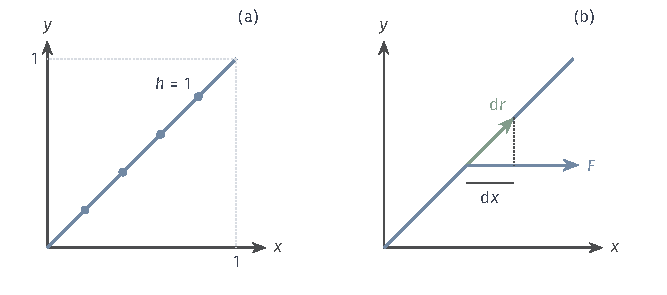
\includegraphics[width=112mm]{figures/01-mathematical-preliminaries-upper/01-mathematical-language-combinatorics-analysis-optimization/tikz/chapter3-concept-processes/line-density-work.pdf}
 \caption{路径均为$\gamma(t)=(t,t)^\top$，$0\leq t\leq1$。(a) 常数线密度$h=1$按弧长累计，得到$\sqrt2$。(b) 常向量场$\bm F=(1,0)^\top$只取位移的水平分量，做功为$1$；图中$\mathrm dx$是$\mathrm d\bm r$的水平投影。相同路径、不同被积对象和权重给出不同积分。}
 \label{fig:analysis-process-line-density-work}
\end{figure}

\subsubsection{积分的基本性质}

下列公式均由内积的线性和一元勒贝格积分的相应性质得到。以下说$\bm F$沿$\gamma$可积，是指定义中的可测性与绝对可积条件成立，因而相应的有向积分有限。前三条说明功对力是线性的，接下来三条说明功怎样随路径的拼接、方向和参数化变化，最后一条估计功的大小。

\paragraph{加法}

若$\bm F$和$\bm G$沿$\gamma$可积，则$\bm F+\bm G$也沿$\gamma$可积，且
\[
 \int_\gamma(\bm F+\bm G)\cdot\mathrm d\bm r
 =\int_\gamma\bm F\cdot\mathrm d\bm r+\int_\gamma\bm G\cdot\mathrm d\bm r.
\]
这里先把两个向量场相加，再与位移取内积。两个力同时作用时，合力做的功等于两个力各自做功之和。

\paragraph{减法}

把$\bm G$换成相反场$-\bm G$，由加法得到
\[
 \int_\gamma(\bm F-\bm G)\cdot\mathrm d\bm r
 =\int_\gamma\bm F\cdot\mathrm d\bm r-\int_\gamma\bm G\cdot\mathrm d\bm r.
\]
可积性保证两个积分都有限，所以可以相减。

\paragraph{数乘}

对实数$c$，有
\[
 \int_\gamma c\bm F\cdot\mathrm d\bm r
 =c\int_\gamma\bm F\cdot\mathrm d\bm r.
\]
力放大$c$倍，功也放大$c$倍；$c<0$时力反向，功变号。路径本身没有改变。

\paragraph{路径拼接}

若$\gamma_1$和$\gamma_2$首尾相接，则
\[
 \int_{\gamma_1*\gamma_2}\bm F\cdot\mathrm d\bm r
 =\int_{\gamma_1}\bm F\cdot\mathrm d\bm r
 +\int_{\gamma_2}\bm F\cdot\mathrm d\bm r.
\]
先走一段再走一段，总功是两段的功之和。因此分段光滑路径可以逐段计算，但每段都必须按这次行进的实际方向参数化。

\paragraph{方向反转}

记反向路径为$\gamma^{-}(u)=\gamma(a+b-u)$，$a\leq u\leq b$，它从$\gamma(b)$出发、沿原路走回$\gamma(a)$。由链式法则，它的速度是$-\gamma'(a+b-u)$，与原速度相反；再用一元换元$t=a+b-u$，得到
\[
 \int_{\gamma^{-}}\bm F\cdot\mathrm d\bm r
 =-\int_\gamma\bm F\cdot\mathrm d\bm r.
\]
顺风骑车时风做正功，沿原路逆风骑回来，风在每一段都做等量的负功。第一类积分反向后不变，因为长度始终非负；有向位移反向则改变符号。
特别地，往返路径$\gamma*\gamma^{-}$上的第二类积分为零，而它的长度是$\gamma$的两倍；示例~\ref{ex:analysis-diagonal-segment-paths}中的$\rho$就是对角线段上的这种往返路径。

\paragraph{重参数化}

若$t=\sigma(u)$为端点相配、严格递增的分段$C^1$微分同胚，则
$(\gamma\circ\sigma)'(u)=\gamma'(\sigma(u))\sigma'(u)$。在参数公式中应用换元$t=\sigma(u)$，得到
\[
 \int_{\gamma\circ\sigma}\bm F\cdot\mathrm d\bm r
 =\int_\gamma\bm F\cdot\mathrm d\bm r.
\]
也就是说，功只取决于经过哪些位置、朝哪个方向经过，与走得快慢无关。
与第一类积分不同，这里乘的是$\sigma'$本身而不是$|\sigma'|$。严格递减的重参数化把路径变成反向路径，换元后积分上下限交换，积分因此变号。重参数化也不改变经过的次数，同一段路重复走两次时，两次的功都会计入。

\paragraph{绝对值不等式}

由积分的三角不等式和Cauchy--Schwarz不等式$|\bm F^\top\bm\tau|\leq\lVert\bm F\rVert_2$可得
\[
 \left|\int_\gamma\bm F\cdot\mathrm d\bm r\right|
 \leq\int_\gamma\lVert\bm F\rVert_2\,\mathrm ds.
\]
功的绝对值不超过力的大小沿路程的累计；当力处处沿前进方向时取等号。若力的大小不超过$M$，路径长为$\ell$，功的绝对值便不超过$M\ell$。
右侧为$+\infty$时，不等式仍成立，但不能用来证明左侧有限。

\subsubsection{积分的计算}

计算第二类路径积分时，按行进方向参数化路径，把场值与速度向量取内积，再做一元积分。与第一类积分相比，这里乘的是速度向量而不是速率。
先用图~\ref{fig:analysis-process-line-density-work}右图中的常力检验这一步骤。
\begin{example}[常力沿对角线段做功]
取常向量场$\bm F=(1,0)^\top$与对角线段$\gamma(t)=(t,t)^\top$，$0\leq t\leq1$。速度为$(1,1)^\top$，被积函数为$1\cdot1+0\cdot1=1$，所以
\[
 \int_\gamma\bm F\cdot\mathrm d\bm r=\int_0^1 1\,\mathrm dt=1.
\]
\end{example}
同一路径的长度为$\sqrt2$。功为$1$而不是$\sqrt2$，是因为水平方向的力只对位移的水平分量做功，而线段的水平跨度是$1$。

再看地面附近的重力。它同样是常向量场，这次让路径任意弯曲。
\begin{example}[重力做功只取决于高度差]
\label{ex:analysis-gravity-work}
设质量为$m$的物体沿分段$C^1$平面路径$\gamma(t)=(x(t),y(t))^\top$，$a\leq t\leq b$，从高度$y(a)$移动到高度$y(b)$，所受重力为$\bm F=(0,-mg)^\top$。被积函数为$\bm F(\gamma(t))^\top\gamma'(t)=-mg\,y'(t)$。在每个光滑段上用一元基本定理，再把各段相加，得到
\[
 \int_\gamma\bm F\cdot\mathrm d\bm r
 =\int_a^b(-mg)\,y'(t)\,\mathrm dt=-mg\bigl(y(b)-y(a)\bigr).
\]
例如质量为$1$千克的物体下降$2$米，即$y(b)-y(a)=-2$，取$g\approx9.8$米每二次方秒，无论沿斜坡还是沿弯曲的滑梯，重力都做功约$9.8\times2=19.6$焦。
\end{example}
被积函数中不含$x'(t)$，水平移动不受重力影响，只有高度变化起作用。这个结果只依赖起点和终点的高度，第~\ref{sec:multivariable-potential-path-independence}节将说明这并非偶然。

对平面图像路径$\gamma(x)=(x,\psi(x))^\top$、$a\leq x\leq b$，其中$\psi$为$C^1$，速度为$(1,\psi'(x))^\top$。$\bm F=(P,Q)^\top$时有
\[
 \int_\gamma\bm F\cdot\mathrm d\bm r
 =\int_a^b\bigl[P(x,\psi(x))+Q(x,\psi(x))\psi'(x)\bigr]\,\mathrm dx.
\]

重力的功与路线无关。下面固定起点和终点，比较两条路线上的功，观察一般向量场是否也如此。
\begin{example}[半圆和直径]
\label{ex:analysis-path-integral-comparison}
取上半圆$\gamma(t)=(\cos t,\sin t)^\top$，$0\leq t\leq\pi$，它从$(1,0)$逆时针走到$(-1,0)$，速度为$(-\sin t,\cos t)^\top$，速率为$1$，故长度$\int_\gamma1\,\mathrm ds=\pi$。另取起点和终点相同的直径$\lambda(t)=(1-2t,0)^\top$，$0\leq t\leq1$，速度为$(-2,0)^\top$。

对常场$(1,0)^\top$，沿上半圆的功为$\int_0^\pi(-\sin t)\,\mathrm dt=-2$，沿直径的功为$\int_0^1(-2)\,\mathrm dt=-2$。两条路线都向左净移动了$2$，水平向右的力在两条路线上做功都是$-2$，恰等于函数$\phi(x,y)=x$在终点与起点的差$-1-1$。

对旋转场$\bm F=(-y,x)^\top$，沿上半圆有$\bm F(\gamma(t))=(-\sin t,\cos t)^\top$，与速度相同，内积为$\sin^2t+\cos^2t=1$，故功为$\pi$：质点一直顺着旋转方向走。
沿直径，$\bm F(\lambda(t))=(0,1-2t)^\top$竖直，而位移水平，内积恒为零，功为$0$。
两条路线端点相同，旋转场做的功却不同。
\end{example}

对常场，功与路线无关；对旋转场，功依赖于路线。沿完整单位圆逆时针一周，质点回到起点，旋转场做功$2\pi$而不是零。图~\ref{fig:analysis-process-rotation-field-paths}画出了旋转场与这两条路线。
\begin{figure}[!htbp]
 \centering
 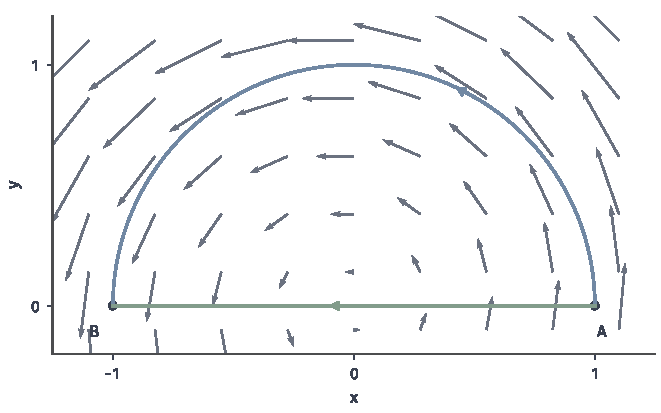
\includegraphics[width=112.0mm]{figures/01-mathematical-preliminaries-upper/01-mathematical-language-combinatorics-analysis-optimization/matplotlib/chapter3-concept-processes/rotation-field-paths.pdf}
 \caption{灰箭头为旋转场$\bm F=(-y,x)^\top$，箭头长度统一缩放为实际场值的$1/4$。两条路径都从$A=(1,0)$到$B=(-1,0)$：蓝色上半圆与场同向，积分为$\pi$；绿色直径上场与位移垂直，积分为零。旋转场处处光滑，端点相同的两条路径上积分仍可不同；下一小节说明势函数给出的路径无关条件。}
 \label{fig:analysis-process-rotation-field-paths}
\end{figure}

\subsection{路径无关与势函数}
\label{sec:multivariable-potential-path-independence}

重力的功只依赖起点和终点的高度，旋转场的功却依赖路线。区别在于：重力的功可以写成某个只依赖位置的量在两端的差，这个量是$-mgy$；旋转场则没有这样的量。
本小节先说明这样的量，即势函数，如何把沿途累计化为端点差；再证明“功与路线无关”反过来也能构造出势函数；最后给出可以直接检查的微分条件，并说明定义域中有洞时，这个条件为什么不再足以保证势函数存在。

\subsubsection{势函数与路径积分}

\paragraph{势函数}

物理中，地面附近质量为$m$的物体在高度$y$处的重力势能为$E_{\mathrm p}(x,y)=mgy$。重力等于势能梯度的相反向量：$-\nabla E_{\mathrm p}=(0,-mg)^\top$。物体下降时势能减少，减少的势能等于重力做的功。
数学中习惯省去负号，取$\phi=-E_{\mathrm p}$，直接要求向量场等于某个标量函数的梯度。
\begin{definition}[势函数]
设$U\subseteq\mathbb R^d$为非空开集，$\bm F:U\to\mathbb R^d$连续。
若存在$\phi\in C^1(U)$使$\bm F=\nabla\phi$，称$\phi$为$\bm F$的\term{势函数}（potential function），称$\bm F$为梯度场，也称保守场。
\end{definition}

梯度指向函数增长最快的方向，所以在梯度非零处，梯度场的箭头指向$\phi$增大的方向，也就是势能$-\phi$减小的方向：重力把物体拉向低处。
例如$\phi(x,y)=x^2+y^2$给出$\bm F(x,y)=(2x,2y)^\top$，箭头从原点向外，因为离原点越远$\phi$越大；常场$(1,0)^\top$的一个势函数是$\phi(x,y)=x$。

给势函数加一个常数，梯度不变，所以势函数不唯一。若$U$还是路径连通的，两个势函数也只能相差一个常数：它们之差的梯度处处为零，路径连通的开集中任意两点都能用域内折线连接，沿折线逐段使用中值公式（定理~\ref{thm:multivariable-scalar-mean-value}），可知这个差在任意两点取值相同。
这与物理中势能的零点可以任选是同一件事：把地面还是桌面取作高度零点，算出的势能差都一样。

“保守”这个名称来自能量守恒。设质量为$m$的质点在力场$\bm F=\nabla\phi$中按牛顿第二定律$m\gamma''(t)=\bm F(\gamma(t))$运动，其中$\gamma$为$C^2$路径。依次用乘积法则、运动方程和链式法则，得到
\[
 \frac{\mathrm d}{\mathrm dt}\Bigl(\tfrac12m\lVert\gamma'(t)\rVert_2^2\Bigr)
 =m\gamma''(t)^\top\gamma'(t)=\nabla\phi(\gamma(t))^\top\gamma'(t)
 =\frac{\mathrm d}{\mathrm dt}\phi(\gamma(t)),
\]
所以动能与势能$-\phi$之和$\frac12m\lVert\gamma'\rVert_2^2-\phi(\gamma)$的导数为零，不随时间变化。最后一个等号已经显示了下面定理的核心：沿路径的功率$\nabla\phi^\top\gamma'$恰是$\phi\circ\gamma$的导数。

\paragraph{路径积分基本定理}

一元基本定理说，导数在区间上的积分等于原函数在两端的差。把势函数与路径复合，得到一元函数$t\mapsto\phi(\gamma(t))$，它的导数恰是第二类路径积分的被积函数，因此一元基本定理直接给出端点差。
直观上，每一小段的功$\nabla\phi^\top\Delta\bm r$近似等于$\phi$在这一小段上的增量，这些增量相加时中间各项逐一抵消，只剩终点值减起点值。
\begin{theorem}[路径积分基本定理]
设$U\subseteq\mathbb R^d$为开集，$\phi\in C^1(U)$，$\gamma:[a,b]\to U$分段$C^1$。则
\begin{equation}
  \int_{\gamma}\nabla\phi\mathbin{\cdot}\mathrm{d}\bm{r}
  =\phi(\gamma(b))-\phi(\gamma(a)).
\label{eq:analysis-line-integral-gradient}
\end{equation}
\end{theorem}
\begin{proof}
在每个光滑参数段$[t_{j-1},t_j]$上，链式法则给出
\[
 (\phi\circ\gamma)'(t)=\nabla\phi(\gamma(t))^\top\gamma'(t).
\]
右侧是连续函数的复合与乘积，在该段上连续，所以对该段使用一元基本定理，得到
$\int_{t_{j-1}}^{t_j}\nabla\phi(\gamma(t))^\top\gamma'(t)\,\mathrm dt=\phi(\gamma(t_j))-\phi(\gamma(t_{j-1}))$。
对$j=1,\dots,n$相加，中间端点的值一正一负逐一抵消，只剩$\phi(\gamma(b))-\phi(\gamma(a))$。
\end{proof}

用势能$E_{\mathrm p}=-\phi$来读，式~\eqref{eq:analysis-line-integral-gradient}说：保守力沿任何路线做的功都等于起点势能减终点势能，即势能的下降量。示例~\ref{ex:analysis-gravity-work}的重力做功就是$\phi(x,y)=-mgy$的情形。

这个定理有两个直接推论。第一，梯度场的积分只依赖端点：两条端点相同的路线，功相同。第二，闭路径的起点与终点重合，所以梯度场沿任意闭路径的积分为零：把书从地上拿到桌上再放回地上，重力在全过程中做的总功为零。
方向反转时端点交换，端点差变号，这与第二类积分的方向反转性质一致。

知道势函数后，计算路径积分不必代入参数。
\begin{example}[用势函数计算沿半圆的积分]
取$\bm F=(2x,2y)^\top$，它的势函数为$\phi(x,y)=x^2+y^2$。路径取示例~\ref{ex:analysis-path-integral-comparison}中的上半圆$\gamma(t)=(\cos t,\sin t)^\top$，$0\leq t\leq\pi$，从$(1,0)$走到$(-1,0)$。由式~\eqref{eq:analysis-line-integral-gradient}，
\[
 \int_\gamma\bm F\cdot\mathrm d\bm r=\phi(-1,0)-\phi(1,0)=1-1=0.
\]
直接代入参数也得到同样结果：$\bm F(\gamma(t))^\top\gamma'(t)=2\cos t\,(-\sin t)+2\sin t\cos t=0$。这个场在圆周上处处沿半径方向，与切线垂直。
\end{example}

第二个推论还可以用来否定势函数的存在。旋转场沿单位圆逆时针一周做功$2\pi\neq0$，所以它在$\mathbb R^2$上没有势函数。

\subsubsection{路径无关的等价判别}

\paragraph{路径无关}

路径积分基本定理说明，有势函数就能推出功与路线无关。要讨论反方向，先把“与路线无关”说准确。比较同一对端点间的不同路线，需要域内任意两点都能用路径连接；对欧氏开集，路径连通时任意两点之间还能选到域内的折线，因而能选到分段光滑路径。
\begin{definition}[路径无关]
设$U\subseteq\mathbb R^d$为非空、开且路径连通的集合，$\bm F:U\to\mathbb R^d$连续。
若对任意$\bm a,\bm b\in U$及域内从$\bm a$到$\bm b$的任意两条分段$C^1$路径，第二类路径积分都相等，称$\bm F$的路径积分与路径无关。
\end{definition}

反方向的想法来自物理中定义势能的办法：选定一个参考点作为势能零点，把力从参考点到某点所做的功取负号，作为该点的势能。只有当这个功与所选路线无关时，这样定义的势能才是一个确定的数。下面的定理说明，路径无关、闭路径积分为零与势函数存在三者等价。
\begin{theorem}[路径无关的等价条件]
设$U\subseteq\mathbb R^d$非空、开且路径连通，$\bm F:U\to\mathbb R^d$连续。下列条件等价：
\begin{enumerate}
 \item 存在$\phi\in C^1(U)$使$\nabla\phi=\bm F$；
 \item $\bm F$的路径积分与路径无关；
 \item 域内每条分段$C^1$闭路径的积分都为零。
\end{enumerate}
\end{theorem}
\begin{proof}
条件1推出条件2，是路径积分基本定理的第一个推论。
条件2推出条件3：设$\gamma$是从$\bm a$出发回到$\bm a$的闭路径。停在$\bm a$不动的常值路径也从$\bm a$到$\bm a$，它的速度为零，积分为零；由路径无关，$\gamma$上的积分也为零。
条件3推出条件2：设$\gamma_1,\gamma_2$都从$\bm a$到$\bm b$。先沿$\gamma_1$走到$\bm b$，再沿$\gamma_2$的反向路径$\gamma_2^-$走回$\bm a$，拼成闭路径$\gamma_1*\gamma_2^-$。由拼接和方向反转性质，
\[
 0=\int_{\gamma_1*\gamma_2^-}\bm F\cdot\mathrm d\bm r
 =\int_{\gamma_1}\bm F\cdot\mathrm d\bm r-\int_{\gamma_2}\bm F\cdot\mathrm d\bm r.
\]

最后由条件2构造势函数。固定参考点$\bm a\in U$，对每个$\bm x\in U$，取域内任意一条从$\bm a$到$\bm x$的分段$C^1$路径，令$\phi(\bm x)$为沿它的积分。路径无关保证这个数不依赖所选路线。
下面计算偏导数。因为$U$开，存在$r>0$使以$\bm x$为中心、半径$r$的球在$U$内。对$0<|h|<r$，到$\bm x+h\bm e_j$的一条路径可以这样选：先沿原来的路径走到$\bm x$，再沿第$j$个坐标方向走线段$t\mapsto\bm x+t\bm e_j$，$t$从$0$到$h$。线段的速度为$\bm e_j$，场与速度的内积是第$j$个分量$F_j$，于是
\[
 \phi(\bm x+h\bm e_j)-\phi(\bm x)
 =\int_0^h F_j(\bm x+t\bm e_j)\,\mathrm dt.
\]
（$h<0$时按有向积分理解。）右侧除以$h$，是$F_j$在这条短线段上的平均值。$F_j$连续，$h\to0$时这个平均值趋于$F_j(\bm x)$，所以$\partial_j\phi(\bm x)=F_j(\bm x)$。
所有偏导数都等于$\bm F$的连续分量，故$\phi\in C^1(U)$且$\nabla\phi=\bm F$，得到条件1。
\end{proof}

证明中的$\phi$正是“从参考点出发做的功”。换一个参考点$\bm a'$，$\phi$只改变一个常数，即从$\bm a'$到$\bm a$的功，这与势能零点可以任选一致。

\subsubsection{势函数存在的微分判别}

\paragraph{交叉偏导相等的必要条件}

路径无关的等价条件把势函数的存在归结为检查所有路径或所有闭路径，实际上无法逐条验证。我们希望找到只需对$\bm F$求导就能检查的条件。
若$\bm F=\nabla\phi$，则$F_j=\partial_j\phi$。当$\bm F$本身是$C^1$时，$\phi$具有连续的二阶偏导数，由定理~\ref{thm:multivariable-mixed-partials}，混合偏导可以交换次序，于是$\bm F$的分量之间必须满足一组关系。
\begin{theorem}[保守场的必要条件]
设$U\subseteq\mathbb R^d$为开集，$\bm F\in C^1(U;\mathbb R^d)$。
若$\bm F=\nabla\phi$，其中$\phi\in C^1(U)$，则对所有$i,j$和$\bm x\in U$，有
\[
 \partial_iF_j(\bm x)=\partial_jF_i(\bm x).
\]
\end{theorem}
\begin{proof}
由$\partial_j\phi=F_j\in C^1(U)$可知$\phi\in C^2(U)$，因此
$\partial_iF_j=\partial_i\partial_j\phi=\partial_j\partial_i\phi=\partial_jF_i$。
\end{proof}

在平面中，记$\bm F=(P,Q)^\top$，条件只有一个：$\partial_xQ=\partial_yP$。差$\partial_xQ-\partial_yP$有清楚的几何含义：它度量向量场在一点附近的旋转程度。

为看出这一点，计算沿一个小正方形边界的环流。设正方形为$[x_0,x_0+\delta]\times[y_0,y_0+\delta]$，按逆时针方向行走。下边向右，贡献$\int_{x_0}^{x_0+\delta}P(x,y_0)\,\mathrm dx$；上边向左，贡献$-\int_{x_0}^{x_0+\delta}P(x,y_0+\delta)\,\mathrm dx$。$P$在上下两边相差约$\partial_yP\,\delta$，所以这两项之和约为$-\partial_yP\cdot\delta\cdot\delta$。同理，右边向上、左边向下，两者的贡献之和约为$\partial_xQ\cdot\delta^2$。
因此小正方形的环流约为$(\partial_xQ-\partial_yP)\,\delta^2$，即单位面积上的环流约为$\partial_xQ-\partial_yP$，下面称它为旋转率。

保守场沿每条闭路径做功为零，小正方形也不例外，所以旋转率必须处处为零，这与上面的必要条件一致。这里只是近似推理；沿区域边界的环流与区域内旋转率的精确关系是Green公式，见定理~\ref{thm:multivariable-green}。

两个例子可以对照。场$(2x,2y)^\top$满足$\partial_xQ=0=\partial_yP$，它确实有势函数$x^2+y^2$。旋转场$(-y,x)^\top$有$\partial_xQ-\partial_yP=1-(-1)=2\neq0$，它在每一点附近都在旋转，由上面的必要条件，它在任何非空开集上都没有势函数。这与单位圆上环流为$2\pi$的计算一致：$2\pi$恰是旋转率$2$乘单位圆盘的面积$\pi$。

\paragraph{星形域上的充分条件}

交叉偏导相等只说明每个小区域内没有旋转，它是局部条件；势函数却要在整个定义域上用一个函数表示。要从局部条件得到全局结论，还需要对定义域本身加条件。

一个便于直接构造的条件是星形：若存在$\bm a\in U$，使从$\bm a$到每个$\bm x\in U$的整条线段都在$U$内，称$U$关于$\bm a$星形。凸开集满足这一条件，整个$\mathbb R^d$也满足。
在星形域上，可以沿用路径无关等价条件证明中“从参考点出发做功”的办法定义势函数，并且总沿直线段从$\bm a$走到$\bm x$。
\begin{theorem}[星形域上势函数的构造]
设$U\subseteq\mathbb R^d$为关于$\bm a$星形的开集，$\bm F\in C^1(U;\mathbb R^d)$，且对所有$i,j$有$\partial_iF_j=\partial_jF_i$。则
\[
 \phi(\bm x)=\int_0^1\bm F(\bm a+t(\bm x-\bm a))^\top(\bm x-\bm a)\,\mathrm dt
\]
属于$C^1(U)$且满足$\nabla\phi=\bm F$。因此$\bm F$的路径积分与路径无关。
\end{theorem}
\begin{proof}
记$\bm z=\bm x-\bm a$。$\phi(\bm x)$是$\bm F$沿线段$t\mapsto\bm a+t\bm z$，$0\leq t\leq1$，的第二类路径积分，因为这条线段的速度恒为$\bm z$。
固定$\bm x$时，这条线段是$U$内的紧集，因而它的一个足够小的紧邻域仍在$U$内；当$\bm x$在一个小范围内变动时，相应线段都留在这个紧邻域中。
$\bm F$及其一阶偏导在紧邻域上连续因而有界，所以被积函数对$x_j$的偏导数有不依赖$t$的上界，可以用式~\eqref{eq:analysis-differentiate-under-integral}在积分号下对$x_j$求导。

被积函数为$\sum_iF_i(\bm a+t\bm z)z_i$。对$x_j$求导时，$z_j$对$x_j$的导数为$1$，$F_i(\bm a+t\bm z)$对$x_j$的导数由链式法则为$t\,\partial_jF_i(\bm a+t\bm z)$，所以偏导数为
\[
 F_j(\bm a+t\bm z)+t\sum_i z_i\partial_jF_i(\bm a+t\bm z).
\]
交叉偏导条件把$\partial_jF_i$换成$\partial_iF_j$，而$\sum_iz_i\partial_iF_j(\bm a+t\bm z)$正是$t\mapsto F_j(\bm a+t\bm z)$的导数，于是
\[
 \begin{aligned}
 F_j(\bm a+t\bm z)+t\sum_i z_i\partial_jF_i(\bm a+t\bm z)
 &=F_j(\bm a+t\bm z)+t\sum_i z_i\partial_iF_j(\bm a+t\bm z)\\
 &=\frac{\mathrm d}{\mathrm dt}\bigl[tF_j(\bm a+t\bm z)\bigr].
 \end{aligned}
\]
对$t$从$0$积分到$1$，由一元基本定理得$\partial_j\phi(\bm x)=1\cdot F_j(\bm a+\bm z)-0=F_j(\bm x)$。
这些偏导连续，所以$\phi\in C^1(U)$；路径无关由前一定理得到。
\end{proof}

用这个构造可以求出一个具体平面场的势函数。
\begin{example}[沿线段构造势函数$x^2y$]
取$\bm F(x,y)=(2xy,x^2)^\top$，即$P=2xy$，$Q=x^2$。它定义在整个平面上，分量都是多项式，属于$C^1$，并且$\partial_yP=2x=\partial_xQ$。整个平面关于$\bm a=\bm0$星形，代入构造公式，
\[
 \phi(x,y)=\int_0^1\bigl[2(tx)(ty)\,x+(tx)^2\,y\bigr]\,\mathrm dt
 =\int_0^13t^2x^2y\,\mathrm dt=x^2y.
\]
直接求导可验证$\nabla\phi=(2xy,x^2)^\top$。于是这个场沿任何从$(0,0)$到$(1,2)$的分段$C^1$路径做功都等于$\phi(1,2)-\phi(0,0)=2$。
\end{example}
星形域上的构造不依赖猜测：交叉偏导相等时，沿线段积分就给出势函数，任意路径上的功随之化为端点差。

\paragraph{穿孔平面上的反例}

星形域的条件不能省略。下面的向量场在原点以外处处满足交叉偏导条件，在穿孔平面上却没有势函数。
\begin{example}[穿孔平面上的涡旋场]
\label{ex:analysis-punctured-plane-vortex}
在穿孔平面$\mathbb R^2\setminus\{\bm0\}$上考虑
\[
 \bm F(x,y)=\left(-\frac{y}{x^2+y^2},\frac{x}{x^2+y^2}\right)^\top ,
\]
记它的两个分量为$P,Q$。它与旋转场$(-y,x)^\top$方向相同，都沿逆时针方向与以原点为圆心的圆相切，但大小改为到原点距离的倒数：离原点越近转得越快，类似于绕一根细涡管旋转的水流。原点处它没有定义。

先检查交叉偏导。由商的求导法则，
\[
 \begin{aligned}
 \partial_yP&=-\frac{(x^2+y^2)-y\cdot2y}{(x^2+y^2)^2}=\frac{y^2-x^2}{(x^2+y^2)^2},\\
 \partial_xQ&=\frac{(x^2+y^2)-x\cdot2x}{(x^2+y^2)^2}=\frac{y^2-x^2}{(x^2+y^2)^2},
 \end{aligned}
\]
两者在穿孔平面上处处相等，所以这个场在原点以外的每一点附近都没有旋转。

再沿单位圆$\gamma(t)=(\cos t,\sin t)^\top$，$0\leq t\leq2\pi$，逆时针走一周。在单位圆上$x^2+y^2=1$，$\bm F(\gamma(t))=(-\sin t,\cos t)^\top$与速度相同，内积为$1$，积分为$2\pi$。
闭路径积分不为零，由路径无关的等价条件，$\bm F$在穿孔平面上没有势函数。
\end{example}

交叉偏导相等这个局部条件，在这里没能给出全局的势函数。这与星形域上的定理并不矛盾：穿孔平面不是星形域，对任一点$\bm a\neq\bm0$，从$\bm a$到$-\bm a$的线段都经过原点。问题出在原点这个洞上，可以从两个角度理解。

第一，局部的势函数是极角。在不含原点的区域上，若能连续地选取点$(x,y)$的极角$\theta$，使$x=r\cos\theta$、$y=r\sin\theta$，其中$r=\sqrt{x^2+y^2}$，则直接求导可得$\nabla\theta=\bm F$。例如在右半平面$x>0$上取$\theta=\arctan(y/x)$，有$\partial_x\theta=-y/(x^2+y^2)$，$\partial_y\theta=x/(x^2+y^2)$。
在更大的区域，即去掉负半轴的平面$\mathbb R^2\setminus\{(x,0)^\top:x\leq0\}$上，取$\theta\in(-\pi,\pi)$，它连续且仍满足$\nabla\theta=\bm F$；这个区域关于$(1,0)$星形，与星形域上的定理一致。

但在整个穿孔平面上无法连续地选取极角：从$(1,0)$出发绕原点逆时针一周回到$(1,0)$，极角连续地增加了$2\pi$，起点和终点处的“势函数值”对不上。单位圆上的积分$2\pi$正是极角的这个增量。
具体地，从$(1,0)$到$(-1,0)$，沿上半圆极角从$0$增加到$\pi$，积分为$\pi$；沿下半圆$(\cos t,-\sin t)^\top$，$0\leq t\leq\pi$，极角从$0$减少到$-\pi$，积分为$-\pi$。两条路线的功相差$2\pi$，恰是绕原点一圈的积分。
不绕原点的闭路径则没有这个问题。例如以$(3,0)$为圆心、半径为$1$的圆整个落在右半平面中，那里$\theta$是势函数，沿它的积分为零。

第二，从小正方形的环流看。交叉偏导相等说明每个小正方形的环流近似为零。若一条闭路径围住的区域整个在定义域内，可以把这个区域划分成许多小正方形；相邻正方形的公共边被沿相反方向各走一次，贡献相互抵消，只剩外边界，于是外边界的环流也为零。这一推理的精确形式就是Green公式（定理~\ref{thm:multivariable-green}），它要求向量场在整个被围区域附近都有定义且连续可微。

单位圆围住的圆盘却包含原点，那里$\bm F$没有定义，无法这样填满。全部旋转都集中在原点这一个洞里。对夹在两条绕原点闭路径之间、不含原点的环形区域作同样的划分，可知两条路径上的环流相等；所以绕原点逆时针一周的简单闭路径，积分都是$2\pi$，而围住的区域不含原点的闭路径，积分为零。

相比之下，星形域上不会出现这样的洞：任何闭路径都可以沿线段向中心点$\bm a$连续收缩而不离开定义域。这从几何上解释了，为什么在星形域上交叉偏导条件已经足以保证势函数存在。

\FloatBarrier

\par\Needspace{10\baselineskip}
\section{曲面积分}
\label{sec:analysis-surface-integration}

路径积分按长度累计细线上的量，曲面积分则按面积累计薄片上的量。
这里有两个不同的被积对象：标量函数$h:S\to\mathbb R$给出每单位面积的密度，
向量场$\bm F:S\to\mathbb R^3$给出空间中各点处有大小和方向的作用。
前者乘面积得到质量等总量；后者先取法向分量，再乘面积得到穿过曲面的通量。
二者都需要由参数化求出面积元，但只有通量需要选定法向。
本节先建立共同的曲面几何，再分别研究两类积分的定义、可积性、性质和计算。
全部积分采用勒贝格积分；参数曲面、面积元和通量的标准构造可参考\scite{math-openstax-calculus3}。

\subsection{参数曲面与面积}

空间中的曲面通常不能用一个平面区域直接代替，但可以用两个参数标记曲面上的点。
参数化的作用是把曲面上的累计转回二维参数域，同时用面积权重补偿曲面的倾斜和伸缩。

\subsubsection{曲面的参数化}

\paragraph{正则曲面片}

曲面的参数化是向量值映射：输入两个实数，输出三个空间坐标。
为了让它描述一张面，需要两个参数方向真正独立，并避免把同一片面重复计算。

\begin{definition}[正则参数曲面片]
\label{def:analysis-regular-surface-patch}
设$E\subseteq\mathbb R^2$是有界闭区域，$E=\overline{E^\circ}$且二维勒贝格测度$m_2(\partial E)=0$。
设$\bm r$在$E$的一个开邻域内是$C^1$映射，写成
\[
 \bm r(u,v)=(x(u,v),y(u,v),z(u,v))^\top\in\mathbb R^3.
\]
若不同参数只有在都属于$\partial E$时才允许表示同一点，
且两个偏导向量$\bm r_u,\bm r_v$在$E^\circ$上处处线性无关，则称$\bm r$为一个正则曲面片的参数化，曲面片记为$S=\bm r(E)$。
参数边界允许产生接缝或退化点；这些边界部分按零曲面面积处理。
\end{definition}

这里两个切向量线性无关，是指对任意实数$\alpha,\beta$，
$\alpha\bm r_u+\beta\bm r_v=\bm0$只有在$\alpha=\beta=0$时才成立。

固定$v$而改变$u$得到一条参数曲线，它的速度是$\bm r_u$；固定$u$得到的另一条参数曲线的速度是$\bm r_v$。
二者张成曲面的切平面。这里$\bm r_u,\bm r_v$都是三维向量，
并非某个标量函数的两个偏导数。
例如$\bm r(u,v)=(u,v,u+v)^\top$、$E=[0,1]^2$描述平面$z=x+y$上的一块平行四边形，
两个切向量分别为$(1,0,1)^\top$和$(0,1,1)^\top$。

\paragraph{叉积}

小参数矩形的两条边近似映为$\bm r_u\Delta u$和$\bm r_v\Delta v$。
要求它们张成的平行四边形面积，需要一个同时记录面积和垂直方向的向量运算。
对$\bm a,\bm b\in\mathbb R^3$，定义叉积
\[
 \bm a\times\bm b
 =(a_2b_3-a_3b_2,\ a_3b_1-a_1b_3,\ a_1b_2-a_2b_1)^\top.
\]
它垂直于$\bm a,\bm b$，长度等于两向量张成的平行四边形面积，交换次序则变号。
因此正则性也可以写成$\bm r_u\times\bm r_v\ne\bm0$，
小曲面片的面积近似为$\lVert\bm r_u\times\bm r_v\rVert_2\Delta u\Delta v$。

\subsubsection{曲面面积的表示}

\paragraph{面积元与面积测度}

参数域上的面积$\mathrm du\,\mathrm dv$与曲面上的实际面积通常不同。
把刚才得到的局部面积比作为权重，就能把二维勒贝格测度转成曲面上的面积测度。

\begin{definition}[曲面面积测度]
\label{def:analysis-surface-area-measure}
在上述曲面片上，记$J_S(u,v)=\lVert\bm r_u\times\bm r_v\rVert_2$。
若$A\subseteq S$的原像$\bm r^{-1}(A)\cap E$勒贝格可测，则称$A$为曲面可测集，定义
\[
 \sigma_S(A)=\iint_E\bm1_A(\bm r(u,v))J_S(u,v)\,\mathrm du\,\mathrm dv.
\]
曲面面积元记为$\mathrm dS$，参数表示为
\[
 \mathrm dS=J_S(u,v)\,\mathrm du\,\mathrm dv,
 \qquad \operatorname{area}(S)=\sigma_S(S).
\]
\end{definition}

原像保留集合的补、交和并，而右侧是非负权重下的勒贝格积分，
所以这些曲面可测集构成$\sigma$代数，$\sigma_S$在其上可数可加。
$J_S$在紧集$E$上连续有界，且$m_2(E)<\infty$，故这里的曲面片面积有限。
参数边界的二维测度为零，不贡献面积；边界接缝上的重复参数也不重复累计正面积部分。
前面的斜平面片有$\bm r_u\times\bm r_v=(-1,-1,1)^\top$，
故$J_S=\sqrt3$，其面积为$\sqrt3$，而参数正方形的面积为$1$。


图~\ref{fig:analysis-process-surface-area-stretch}将参数小块与实际斜面小块对应起来，解释叉积长度校正的是哪一个面积。
\begin{figure*}[!htbp]
 \centering
 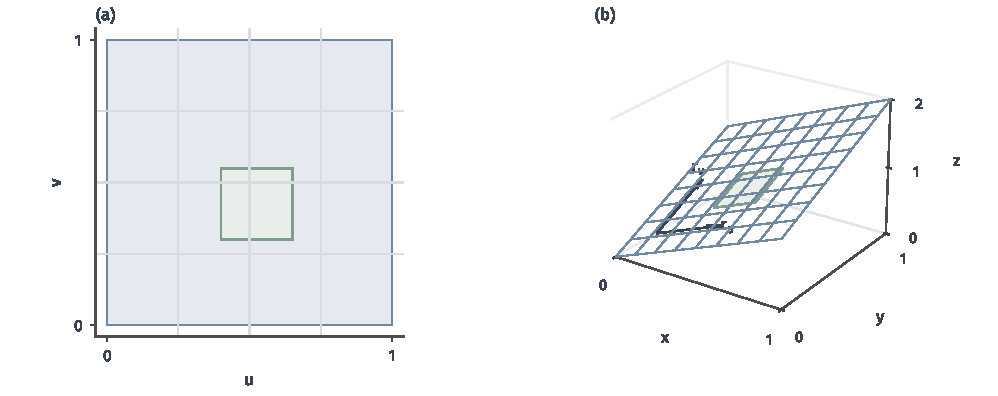
\includegraphics[width=169.0mm]{figures/01-mathematical-preliminaries-upper/01-mathematical-language-combinatorics-analysis-optimization/matplotlib/chapter3-concept-processes/surface-area-stretch.pdf}
 \caption{参数化$r(u,v)=(u,v,u+v)^\top$把单位正方形映为斜平面片，绿色块为同一参数子区间及其像。两切向量$r_u=(1,0,1)^\top$、$r_v=(0,1,1)^\top$在右侧按$0.4$倍画出，叉积长度为$\sqrt3$。每个参数面积都放大$\sqrt3$倍，故不能把$\mathrm du\,\mathrm dv$直接当成$\mathrm dS$。}
 \label{fig:analysis-process-surface-area-stretch}
\end{figure*}

\paragraph{重参数化}

同一块面可以用不同参数标记。要让上面的面积描述曲面本身，
还需证明更换单次覆盖的参数后，面积权重恰好抵消参数域的面积变化。

\begin{theorem}[重参数化下的面积元]
\label{thm:analysis-surface-reparameterization}
设$\bm r:E\to S$满足上述条件，$T:\widetilde E\to E$是参数域之间的双射，
在闭域的开邻域内为$C^1$映射，并在内部是$C^1$微分同胚。
若$\widetilde{\bm r}=\bm r\circ T$仍满足曲面片条件，则
\[
 \begin{aligned}
 \widetilde{\bm r}_\xi\times\widetilde{\bm r}_\eta
 &=\det\bm J_T\,(\bm r_u\times\bm r_v)\circ T,\\
 \widetilde J_S&=(J_S\circ T)|\det\bm J_T|.
 \end{aligned}
\]
两组参数由此给出同一面积测度。
\end{theorem}

\begin{proof}
链式法则给出$\widetilde{\bm r}_\xi=\bm r_u u_\xi+\bm r_v v_\xi$和
$\widetilde{\bm r}_\eta=\bm r_u u_\eta+\bm r_v v_\eta$，其中右端各量在$T(\xi,\eta)$处取值。
利用叉积的双线性、$\bm a\times\bm a=\bm0$和交换次序变号，得到
\[
 \widetilde{\bm r}_\xi\times\widetilde{\bm r}_\eta
 =(u_\xi v_\eta-v_\xi u_\eta)(\bm r_u\times\bm r_v)\circ T.
\]
取长度得到第二式。将它代入任一可测集$A$的面积定义，
二维勒贝格积分的换元公式便把新参数下的积分变回原积分。
\end{proof}

行列式的绝对值保证面积非负；行列式本身的符号则记录参数次序是否翻转，
后面选取通量的法向时还会使用这一信息。
若参数在正面积范围内重复覆盖，参数积分会重复累计，不能直接把它当作单次曲面面积。

\paragraph{分片曲面}

球面、封闭边界或带折角的曲面可能需要多张参数片描述。
本节处理有限分片的情形：各片内部不重叠，交接部分在相邻曲面片中面积均为零，
整个曲面的面积测度由各片面积测度相加。
这样曲面面积和后面的面积积分都可以逐片计算，不需在接缝上补加一项。
无界曲面或不能由这里的有限正则片覆盖的曲面，还需另外处理覆盖和可积性条件。

\subsection{第一类曲面积分}

给定曲面以后，先考虑标量函数$h$在曲面上的累计。
面积测度已经确定了每块薄片的权重，因此可以直接沿用前面建立的测度积分。

\subsubsection{积分的定义和可积性}

\paragraph{按面积的积分}

把面密度乘小片面积再相加，提示我们应当对面积测度积分。
下面的定义既包含连续密度，也允许有跳跃或仅可测的密度。

\begin{definition}[第一类曲面积分]
\label{def:analysis-scalar-surface-integral}
设$h$是$S$上的可测标量函数。
当$h\geq0$时，定义它的\term{第一类曲面积分}（scalar surface integral）为
\begin{equation}
 \int_Sh\,\mathrm dS
 =\iint_Eh(\bm r(u,v))J_S(u,v)\,\mathrm du\,\mathrm dv.
 \label{eq:analysis-scalar-surface-integral}
\end{equation}
该值允许为$+\infty$。一般实值$h$在$\int_S|h|\,\mathrm dS<\infty$时称为曲面可积，
其积分按正、负部分之差定义，仍满足上式。
\end{definition}

取$h=1$得到面积，取非负面密度得到质量。
在前面的单位参数斜平面片上，常数密度$h=2$给出
\[
 \int_S2\,\mathrm dS=\int_0^1\int_0^1 2\sqrt3\,\mathrm du\,\mathrm dv=2\sqrt3.
\]
这一累计不使用法向，因此把曲面的朝向反过来不会改变结果。

\paragraph{可积性的要求}

积分是否有限，取决于函数大小和曲面面积权重共同作用后的累计。
由定义，$h$曲面可积当且仅当参数函数可测且
\[
 \iint_E|h(\bm r(u,v))|J_S(u,v)\,\mathrm du\,\mathrm dv<\infty.
\]
连续函数是一个便于验证的充分情形：$S=\bm r(E)$紧致，连续的$h$有界，
因而$\int_S|h|\,\mathrm dS\leq \sup_S|h|\,\sigma_S(S)<\infty$。
可测性本身并不保证这个绝对积分有限；如果函数在某处无界，仍须检验上式。
这些条件相对于曲面面积，而非三维体积测度；曲面在三维空间中体积为零，并不使面积积分为零。

\subsubsection{积分的性质}

两类标量密度可以叠加，也可以把曲面分开累计。
这些运算由面积测度上的勒贝格积分给出，以下均以相应函数曲面可积为前提。

\paragraph{加法}

对曲面可积的$h,k$，$h+k$也可积，而且
\[
 \int_S(h+k)\,\mathrm dS=\int_Sh\,\mathrm dS+\int_Sk\,\mathrm dS.
\]
可积性由$|h+k|\leq|h|+|k|$得到，等式来自标量勒贝格积分的加法性质。

\paragraph{减法}

对曲面可积的$h,k$，$h-k$也可积，而且
\[
 \int_S(h-k)\,\mathrm dS=\int_Sh\,\mathrm dS-\int_Sk\,\mathrm dS.
\]
这里$|h-k|\leq|h|+|k|$保证绝对可积，等式来自标量勒贝格积分的减法性质。

\paragraph{数乘}

对实数$c$和曲面可积的$h$，$ch$曲面可积，且
\[
 \int_Sch\,\mathrm dS=c\int_Sh\,\mathrm dS.
\]
因为$|ch|=|c||h|$，绝对积分仍有限；数乘公式与参数域上的数乘公式一致。

\paragraph{曲面分割的可加性}

若可测子集$A_j\subseteq S$两两不交，且$h$在$S$上曲面可积，则
\[
 \int_{\bigcup_{j=1}^\infty A_j}h\,\mathrm dS
 =\sum_{j=1}^\infty\int_{A_j}h\,\mathrm dS.
\]
右侧绝对收敛，因为其各项绝对值之和不超过$\int_S|h|\,\mathrm dS$。
有限分片曲面的求和是这一性质的特例；仅在零面积接缝上相交也不影响等式。

\paragraph{单调性}

若曲面可积的$h,k$满足$h\leq k$在曲面面积意义下几乎处处成立，则
\[
 \int_Sh\,\mathrm dS\leq\int_Sk\,\mathrm dS.
\]
因为$k-h$几乎处处非负，其积分非负，应用减法公式即可得到这一不等式。
这里的“几乎处处”允许忽略零曲面面积集合。它不以三维体积衡量例外集合。

\paragraph{绝对值不等式}

对任一曲面可积的$h$，将单调性应用于$-|h|\leq h\leq|h|$得到
\[
 \left|\int_Sh\,\mathrm dS\right|\leq\int_S|h|\,\mathrm dS.
\]
因此绝对值的面积积分给出了原积分大小的上界。

\subsubsection{积分的计算}

计算第一类曲面积分时，先选单次覆盖的参数化，再把$h$与参数化复合，并乘叉积的长度。
若曲面是标量函数$z=\psi(x,y)$在参数域$D$上的图像，
其中$D$满足本节的有界闭域和零测边界条件，$\psi$在$D$的开邻域内为$C^1$，可以直接取
$\bm r(x,y)=(x,y,\psi(x,y))^\top$。计算得
\[
 \bm r_x\times\bm r_y=(-\psi_x,-\psi_y,1)^\top,
\]
所以对曲面可积的$h$有
\[
 \int_Sh\,\mathrm dS
 =\iint_Dh(x,y,\psi(x,y))\sqrt{1+\psi_x^2+\psi_y^2}\,\mathrm dx\,\mathrm dy.
\]
根号校正倾斜造成的面积增长。例如$z=ax+by+c$在单位圆盘上方的部分面积为
$\pi\sqrt{1+a^2+b^2}$。若无法向同一坐标平面单值投影，则需换参数化或分片。

半径$R>0$的球面可以取参数
\[
 \begin{gathered}
 \bm r(\varphi,\theta)
 =(R\sin\varphi\cos\theta,R\sin\varphi\sin\theta,R\cos\varphi)^\top,\\
 0\leq\varphi\leq\pi,\quad 0\leq\theta\leq2\pi.
 \end{gathered}
\]
参数域内部正则且单次覆盖，叉积长度为$R^2\sin\varphi$。
两极与经线接缝来自参数边界，不贡献面积；不用在两极把叉积归一化。
因此
\[
 \operatorname{area}(S)
 =\int_0^{2\pi}\int_0^\pi R^2\sin\varphi\,\mathrm d\varphi\,\mathrm d\theta
 =4\pi R^2.
\]

\subsection{第二类曲面积分}

现在改变被积对象，考虑向量场$\bm F:S\to\mathbb R^3$穿过曲面的累计。
面积只给出小片的大小，尚未规定“穿过”的正方向；要取法向分量，必须先选定曲面的朝向。

\subsubsection{曲面的定向}

\paragraph{单位法向量}

正则点的切平面有两个相反的单位法向量，选择哪一个决定通量的正负。
参数次序提供一个局部选择：在$E^\circ$上令
\[
 \bm n(\bm r(u,v))
 =\frac{\bm r_u\times\bm r_v}{\lVert\bm r_u\times\bm r_v\rVert_2}.
\]
这个向量长度为$1$，并且垂直于两个参数方向；交换$u,v$会把它反转。
参数边界上若叉积退化，不使用这个商定义法向。该部分面积为零，不影响通量积分。

\paragraph{定向与可定向性}

每一点分别选择正负还不够，选择需要在一张面上相容。
相容的连续选择使相邻位置的正方向保持一致，这就是曲面的定向。

\begin{definition}[曲面的定向]
\label{def:analysis-surface-orientation}
在光滑曲面$S$上连续选取一个单位法向量场$\bm n$，称为给曲面\term{定向}（orientation）。
存在这种选择的曲面称为可定向曲面；$\bm n$和$-\bm n$给出相反的定向。
分片光滑曲面要求各片的选择相容：光滑接合处选择同一侧法向，
折角处按整个曲面的同一侧约定，但不要求接缝上存在唯一法向。
\end{definition}

例如图像曲面可以选向上法向，球面可以选外法向。
闭曲面围成规则区域时，外法向指向区域外侧。
不能在全曲面相容选择法向时，面积积分仍有定义，但不能使用这里的全局定向通量。

\subsubsection{积分的定义和可积性}

\paragraph{通量积分}

选定$\bm n$以后，$\bm F^\top\bm n$是一个标量：它表示场沿法向穿过单位面积的分量。
对这个标量作面积积分，就得到有正负号的通量。

\begin{definition}[第二类曲面积分]
\label{def:analysis-surface-flux-integral}
设可定向曲面$S$已选定单位法向$\bm n$，向量场$\bm F:S\to\mathbb R^3$的法向分量可测，且
$\int_S|\bm F^\top\bm n|\,\mathrm dS<\infty$。
定义\term{第二类曲面积分}（flux integral），也称通量积分，为
\begin{equation}
 \int_S\bm F^\top\bm n\,\mathrm dS
 =\iint_E\bm F(\bm r(u,v))^\top(\bm r_u\times\bm r_v)\,\mathrm du\,\mathrm dv,
 \label{eq:analysis-surface-flux}
\end{equation}
其中参数化的叉积方向须与所选$\bm n$一致；若方向相反，右端需乘$-1$。
分片曲面的通量按相容定向逐片相加。
\end{definition}

通量为正表示沿所选法向的净贡献，为负表示逆法向的净贡献。
它的结果是一个标量，不能与向量场三个分量分别作面积积分所得的向量混为一谈。
若$\bm F=(P,Q,R)^\top$，有向面积分量也可记为
\[
 \bm n\,\mathrm dS=(\mathrm dy\,\mathrm dz,\mathrm dz\,\mathrm dx,\mathrm dx\,\mathrm dy)^\top,
\]
从而把通量写为$\int_SP\,\mathrm dy\,\mathrm dz+Q\,\mathrm dz\,\mathrm dx+R\,\mathrm dx\,\mathrm dy$。
这些分量代表有向投影面积，其符号由法向决定。


图~\ref{fig:analysis-process-normal-projection}在一个法向截面内分解场值，说明通量只累计哪一部分。
\begin{figure}[!htbp]
 \centering
 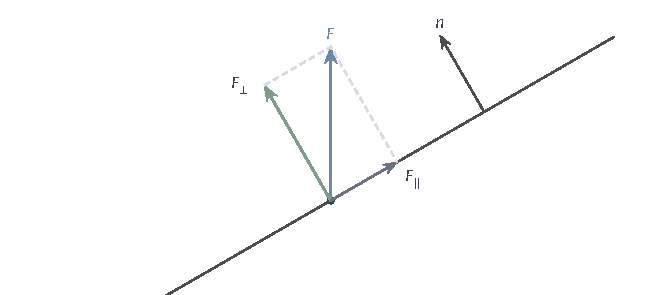
\includegraphics[width=112mm]{figures/01-mathematical-preliminaries-upper/01-mathematical-language-combinatorics-analysis-optimization/tikz/chapter3-concept-processes/normal-projection.pdf}
 \caption{黑斜线表示局部切平面的一个截面，$n$为所选单位法向。向量$F$分为$F_\perp=(F^\top n)n$与切向部分$F_\parallel$；通量使用有符号标量$F^\top n$乘面积，切向部分不贡献。将$n$改为$-n$时标量分量变号，但投影向量$F_\perp$不变，这与直接把场反向不同。}
 \label{fig:analysis-process-normal-projection}
\end{figure}

\paragraph{可积性的要求}

通量只累计法向分量，因此其有限可积性的准确条件是
\[
 \iint_E
 \left|\bm F(\bm r(u,v))^\top(\bm r_u\times\bm r_v)\right|
 \,\mathrm du\,\mathrm dv<\infty.
\]
一个更容易验证的充分条件是$\int_S\lVert\bm F\rVert_2\,\mathrm dS<\infty$。
因为$\lVert\bm n\rVert_2=1$，Cauchy--Schwarz不等式给出
$|\bm F^\top\bm n|\leq\lVert\bm F\rVert_2$。
连续向量场在本节的紧致有限分片曲面上有界，因而满足这一充分条件。
切向分量不进入通量，所以不能把法向分量可积与向量场各分量都可积视为同一个条件。

\subsubsection{积分的性质}

以下运算都在同一曲面、同一法向约定下进行，并假定各法向分量可积。
它们可归结为标量函数$\bm F^\top\bm n$的面积积分，但方向变化需要单独说明。

\paragraph{加法}

向量场相加以后，其法向分量也相加，因此
\[
 \begin{aligned}
 \int_S(\bm F+\bm G)^\top\bm n\,\mathrm dS
 &=\int_S\bm F^\top\bm n\,\mathrm dS\\
 &\quad{}+\int_S\bm G^\top\bm n\,\mathrm dS.
 \end{aligned}
\]
绝对可积性由两项法向分量的绝对值之和控制，积分等式来自标量面积积分的加法性质。

\paragraph{减法}

向量场相减以后，其法向分量也相减，因此
\[
 \begin{aligned}
 \int_S(\bm F-\bm G)^\top\bm n\,\mathrm dS
 &=\int_S\bm F^\top\bm n\,\mathrm dS\\
 &\quad{}-\int_S\bm G^\top\bm n\,\mathrm dS.
 \end{aligned}
\]
两项法向分量绝对可积时，它们的差仍绝对可积，积分等式来自标量面积积分的减法性质。

\paragraph{数乘}

实数$c$可以提出积分号，原因是$(c\bm F)^\top\bm n=c(\bm F^\top\bm n)$，即
\[
 \int_S(c\bm F)^\top\bm n\,\mathrm dS
 =c\int_S\bm F^\top\bm n\,\mathrm dS.
\]
这里缩放的是场，曲面的法向约定保持固定。

\paragraph{曲面分割的可加性}

将$S$分为内部不重叠的有限片$S_1,\ldots,S_N$，并在每片采用原定向的限制，则
\[
 \int_S\bm F^\top\bm n\,\mathrm dS
 =\sum_{j=1}^N\int_{S_j}\bm F^\top\bm n\,\mathrm dS.
\]
零面积接缝不贡献积分；若某片单独反转法向，就改变了被累计的符号，不能仍按同一定向求和。

\paragraph{法向反转}

在场和曲面不变时，把$\bm n$换成$-\bm n$会使通量变号：
\[
 \int_S\bm F^\top(-\bm n)\,\mathrm dS
 =-\int_S\bm F^\top\bm n\,\mathrm dS.
\]

\paragraph{重参数化}

更换参数时，保持已选定的几何法向。重参数化定理表明，参数叉积多出$\det\bm J_T$，
而区域换元使用$|\det\bm J_T|$；若变换翻转参数方向，必须同时校正叉积相对于所选法向的符号。
固定曲面的定向并完成这一校正，通量便与参数选择无关。

\subsubsection{积分的计算}

计算通量时，先固定法向，再选与之相容的参数化，最后累计$\bm F$与有向面积向量的内积。
对于图像曲面$z=\psi(x,y)$，前面已求出叉积$(-\psi_x,-\psi_y,1)^\top$，它的第三分量为正。
因此取向上法向时，对$\bm F=(P,Q,R)^\top$有
\[
 \int_S\bm F^\top\bm n\,\mathrm dS
 =\iint_D(-P\psi_x-Q\psi_y+R)(x,y,\psi(x,y))\,\mathrm dx\,\mathrm dy.
\]
取向下法向则在右侧加负号。这一式直接使用有向面积，不能再额外乘一次叉积长度。

在平面片$\bm r(u,v)=(u,v,u+v)^\top$上，向上单位法向为$(-1,-1,1)^\top/\sqrt3$。
对竖直单位场$\bm F=(0,0,1)^\top$，场与参数叉积的内积为$1$，故
\[
 \int_S\bm F^\top\bm n\,\mathrm dS
 =\int_0^1\int_0^1 1\,\mathrm du\,\mathrm dv=1.
\]
其面积为$\sqrt3$，但法向分量只有$1/\sqrt3$。
同样地，平面$z=ax+by+c$在单位圆盘上方的部分对该场的向上通量为$\pi$，
等于水平投影面积；它的实际面积则为$\pi\sqrt{1+a^2+b^2}$。

对半径$R$的球面，前面采用$(\varphi,\theta)$次序的参数叉积指向外侧。
若$\bm F(\bm x)=\bm x/R$，则球面上的$\bm F$恰等于外单位法向，故
\[
 \int_S\bm F^\top\bm n\,\mathrm dS
 =\int_S1\,\mathrm dS=4\pi R^2.
\]
内向通量为$-4\pi R^2$。这次面积与外向通量相等，是因为法向分量处处为$1$；
下一节再用空间区域内部的散度累计核对同一个通量。

\FloatBarrier

\section{三类积分之间的关系}
\label{sec:multivariable-boundary-relations}

一元微积分基本定理说，若$f$在$[a,b]$上连续可微，则导数$f'$在区间上的积分等于$f(b)-f(a)$：区间内部各点的变化率累计起来，只剩下两个端点上的函数值。
区间的边界就是这两个端点，所以$f(b)-f(a)$也可以读成带符号的边界求和：右端点记正号，左端点记负号。
路径积分基本定理（式~\eqref{eq:analysis-line-integral-gradient}）把同样的关系搬到路径上：梯度场沿路径的积分，等于势函数在终点与起点的值之差。

本节把这种“内部导数的累计等于边界上的累计”的关系推广到平面区域、空间区域和曲面。
三种推广共用一个思路。先把对象切成许多小块；在每个小块上，某个导数乘小块的大小，近似等于向量场沿小块边界的累计。
相邻两块的公共边界被两块各算一次，两次的方向相反，相加后抵消，最后只剩下整个对象的外边界。
按边界的类型，本节回答三个问题：平面区域上的积分何时等于边界路径积分，这是Green公式；空间区域上的积分何时等于边界曲面积分，这是Gauss公式；曲面上的积分何时等于曲面边界的路径积分，这是Stokes公式。

这些公式中的被积对象不能互换。沿边界的环流累计向量场的切向分量，对应的内部量是旋度，它衡量场绕一点旋转的强度；
穿过边界的通量累计向量场的法向分量，对应的内部量是散度，它衡量场从一点向外发散的强度。

为此，本节先定义这两种导数以及Laplace算子，并说明它们的物理含义；再规定边界的方向；最后给出各公式的条件、推导和例子。
所有区域积分以及路径、曲面的参数积分均采用勒贝格积分。经典公式的组织参考向量微积分教材\scite{math-openstax-calculus3}。

\subsection{积分公式中的微分算子}

定义~\ref{def:multivariable-gradient}把标量函数的各个一阶偏导数排成梯度。现在考虑开集$U$上的向量场$\bm F$，不妨把它想成流体的速度场：$\bm F(\bm x)$是流体在位置$\bm x$处的速度。
对这样的场，有两个自然的局部问题：在一点附近，流体是净流出还是净流入；流体是否绕这一点打转。
两个问题的答案都由$\bm F$各分量的一阶偏导数决定，但用到的偏导数组合不同。
回答前一个问题的是散度，回答后一个问题的是旋度，二者都以向量场为输入；随后的Laplace算子以标量函数为输入，比较函数在一点的值与周围平均值的差别。

\subsubsection{散度}

\paragraph{小立方体的净流出}

设$\bm F=(F_1,F_2,F_3)^\top$是三维流体的速度场。第~\ref{sec:analysis-surface-integration}节定义的通量只取速度的法向分量，原因如下。
在很短的时间$\Delta t$内，穿过面积为$\Delta S$、单位法向为$\bm n$的一小片曲面的流体，占据一个底面积为$\Delta S$、高约为$(\bm F^\top\bm n)\Delta t$的斜柱；所以单位时间穿过这一小片的流体体积约为$(\bm F^\top\bm n)\Delta S$，速度的切向分量只让流体沿曲面滑动，不贡献穿过量。
现在以点$\bm a$为中心取边长为$h$的小立方体，各面与坐标平面平行，估计单位时间从它流出的净体积。

先看与$x$轴垂直的两张面。右面$x=a_1+h/2$的外法向是$\bm e_1$，场在这张面上的法向分量是$F_1$；用面中心的值代表整张面，流出量约为$F_1(\bm a+\tfrac h2\bm e_1)h^2$。
左面$x=a_1-h/2$的外法向是$-\bm e_1$，流出量约为$-F_1(\bm a-\tfrac h2\bm e_1)h^2$；$F_1>0$时这个量为负，表示沿$x$正方向的流动在左面是流入。两面合计为
\[
 \Bigl[F_1\bigl(\bm a+\tfrac h2\bm e_1\bigr)-F_1\bigl(\bm a-\tfrac h2\bm e_1\bigr)\Bigr]h^2
 \approx \partial_1F_1(\bm a)\,h\cdot h^2,
\]
这里用偏导数乘距离$h$近似了$F_1$在两张面中心之间的差。
若$F_1$沿$x$方向增大，从右面流出的比从左面流入的多，这对面贡献正的净流出；若$F_1$沿$x$方向不变，流入与流出恰好相等。

另外两对面同样分别给出约$\partial_2F_2(\bm a)h^3$和$\partial_3F_3(\bm a)h^3$。六张面合计后除以体积$h^3$，得到
\[
 \frac{\text{小立方体的净流出}}{\text{小立方体的体积}}
 \approx\partial_1F_1(\bm a)+\partial_2F_2(\bm a)+\partial_3F_3(\bm a).
\]
这里只做了一阶近似。在Gauss公式（定理~\ref{thm:analysis-divergence-theorem}）之后将证明，当$\bm F$连续可微且$h\to0$时，左侧确实收敛到右侧。右侧的偏导数之和称为散度。
\begin{definition}[散度]
\label{def:multivariable-divergence}
设$U\subseteq\mathbb R^d$为开集，$\bm F=(F_1,\ldots,F_d)^\top:U\to\mathbb R^d$的各分量一阶偏导数存在。
$\bm F$的\term{散度}（divergence）是标量函数
\[
 \operatorname{div}\bm F
 =\nabla\mathbin{\cdot}\bm F
 =\sum_{j=1}^d\partial_jF_j.
\]
\end{definition}

\paragraph{源的强度}

按小立方体上的推导，散度是单位体积的净流出率，可以理解为一点处“源”的强度。
$\operatorname{div}\bm F(\bm a)>0$表示$\bm a$附近像有一个源，流体在这里产生并向外流走；$\operatorname{div}\bm F(\bm a)<0$表示这里像一个汇，流入的多于流出的；散度为零表示流入与流出平衡。
若流体不可压缩，内部又没有注入或抽出流体的源和汇，则每个小体积的流入量都等于流出量，速度场的散度处处为零。

下面三个场分别对应均匀膨胀、绕轴转动和整体平移，可以用来检验这一解释。
\begin{example}[径向场、旋转场与常场的散度]
三维径向场$\bm F(x,y,z)=(x,y,z)^\top$满足$\partial_xF_1=\partial_yF_2=\partial_zF_3=1$，所以$\operatorname{div}\bm F=1+1+1=3$：流体从各处均匀地向外膨胀，每单位体积每单位时间多出$3$个单位体积的流体。

旋转场$\bm G(x,y,z)=(-y,x,0)^\top$的第一分量不含$x$，第二分量不含$y$，第三分量为零，所以$\operatorname{div}\bm G=0+0+0=0$：流体绕$z$轴转动，任何小立方体流入多少就流出多少。

常场$\bm H=(1,0,0)^\top$的各分量都是常数，散度同样为$0$：流体整体平移，每个小立方体从左面流入的量都从右面流出。
\end{example}
旋转场和常场都不是零场，散度却都为零。可见散度为零只表示局部净流出率为零，并不表示向量场为零。

二维场$(P,Q)^\top$的散度相应为$P_x+Q_y$，它是小正方形四条边上的净流出除以面积所得的极限；定理~\ref{thm:multivariable-planar-flux}的平面通量公式使用这一标量函数。

\subsubsection{旋度}

\paragraph{小正方形上的环流}

净流出不能描述绕一点旋转的运动。旋转场$\bm G=(-y,x,0)^\top$的散度为零，但在水平平面内沿以$z$轴上一点为圆心的圆周逆时针走一圈，场始终与行进方向相同，环流不为零。
为了度量一点附近的旋转，先在平面上计算小正方形边界的环流。设平面场为$(P,Q)^\top$，以$\bm a$为中心取边长为$h$的正方形，沿逆时针方向走一圈。

下边从左向右，切向分量是$P$，贡献约$P(\bm a-\tfrac h2\bm e_2)h$；上边从右向左，贡献约$-P(\bm a+\tfrac h2\bm e_2)h$；两者合计约$-\partial_yP(\bm a)h^2$。
右边从下向上，贡献约$Q(\bm a+\tfrac h2\bm e_1)h$；左边从上向下，贡献约$-Q(\bm a-\tfrac h2\bm e_1)h$；两者合计约$\partial_xQ(\bm a)h^2$。四边相加后除以面积$h^2$，得到
\[
 \frac{\text{小正方形边界的逆时针环流}}{\text{小正方形的面积}}
 \approx\partial_xQ(\bm a)-\partial_yP(\bm a).
\]
两项的符号可以这样理解。若$Q$沿$x$方向增大，右边向上的流速比左边大，这一对边推动逆时针转动；若$P$沿$y$方向增大，上边向右的流速比下边大，这一对边推动顺时针转动，所以$\partial_yP$带负号。

在三维空间中，小正方形可以放在分别垂直于三个坐标轴的平面里，行进方向都取从相应坐标轴正方向看的逆时针。
垂直于$z$轴时，平面坐标是$(x,y)$，$(F_1,F_2)$相当于$(P,Q)$，同样的计算给出$\partial_xF_2-\partial_yF_1$；
垂直于$x$轴时，平面坐标的次序是$(y,z)$，$(F_2,F_3)$相当于$(P,Q)$，得到$\partial_yF_3-\partial_zF_2$；
垂直于$y$轴时，平面坐标的次序是$(z,x)$，$(F_3,F_1)$相当于$(P,Q)$，得到$\partial_zF_1-\partial_xF_3$。
这样选取坐标次序，是因为$\bm e_2\times\bm e_3=\bm e_1$、$\bm e_3\times\bm e_1=\bm e_2$：从坐标轴正方向看，第一个平面坐标轴逆时针转过直角得到第二个。
把这三个环流率按$x,y,z$轴的次序排成一个向量，就得到旋度。
\begin{definition}[旋度]
\label{def:multivariable-curl}
设$U\subseteq\mathbb R^3$为开集，$\bm F=(F_1,F_2,F_3)^\top:U\to\mathbb R^3$的各分量一阶偏导数存在。
$\bm F$的\term{旋度}（curl）是向量场
\[
 \operatorname{curl}\bm F=\nabla\times\bm F
 =\begin{pmatrix}
   \partial_yF_3-\partial_zF_2\\
   \partial_zF_1-\partial_xF_3\\
   \partial_xF_2-\partial_yF_1
  \end{pmatrix}.
\]
\end{definition}

\paragraph{旋转的轴与强度}

坐标平面上的三个计算可以推广到任意方向。设$\bm F$连续可微，$\bm n$是单位向量；在过点$\bm a$且垂直于$\bm n$的平面内，取以$\bm a$为中心的小正方形或小圆周，从$\bm n$的箭头一侧看按逆时针行进。
尺寸趋于零时，环流除以所围面积的极限等于$(\operatorname{curl}\bm F)(\bm a)^\top\bm n$。$\bm n$为坐标轴方向时，这就是上面的计算；一般方向的证明放在Stokes公式之后。

由Cauchy--Schwarz不等式，$(\operatorname{curl}\bm F)^\top\bm n\leq\lVert\operatorname{curl}\bm F\rVert_2$；旋度不为零时，等号当且仅当$\bm n$与旋度同向时成立。
所以旋度的方向是局部旋转最强的转轴，其长度是旋转的强度；转向由右手定则确定：右手大拇指沿旋度方向，其余四指弯曲的方向就是转向。

一个物理图像是放进流水中的小桨轮。让桨轮的转轴沿$\bm n$，水流沿轮缘推动各个叶片；桨轮是否转动、往哪边转，取决于沿轮缘的环流，也就是$(\operatorname{curl}\bm F)^\top\bm n$的符号；转轴与旋度平行时转得最快。
这一图像帮助理解定义，但不代替上面的计算。

先用整体转动和径向膨胀检验这一图像。
\begin{example}[刚体旋转与径向膨胀的旋度]
\label{ex:analysis-rigid-rotation-curl}
整体以角速度$\omega$绕$z$轴旋转的流体，速度场为$\bm F=\omega(-y,x,0)^\top$。代入定义，前两个分量$\partial_yF_3-\partial_zF_2$与$\partial_zF_1-\partial_xF_3$都为零，第三个分量为$\partial_x(\omega x)-\partial_y(-\omega y)=2\omega$，所以$\nabla\times\bm F=(0,0,2\omega)^\top$。
特别地，$\omega=1/2$时$\bm F=(-y/2,x/2,0)^\top$，旋度为$(0,0,1)^\top$。

径向场$(x,y,z)^\top$的第$i$个分量只依赖第$i$个坐标，旋度定义中的每个交叉偏导数都为零，所以旋度为零：流体只向外膨胀而不打转。
\end{example}
刚体旋转的旋度沿转轴，长度是角速度的两倍，与桨轮图像一致。不过，旋度与流线是否弯曲并不是一回事，下面两个场从相反的方向说明这一点。
\begin{example}[剪切流与涡旋场]
剪切流$\bm F=(y,0,0)^\top$的流线都是水平直线。它的偏导数中只有$\partial_yF_1=1$不为零，所以$\nabla\times\bm F=(0,0,-1)^\top$。
物理上，上方的水比下方的水向右流得快，桨轮的上缘被推得更多，从$z$轴正方向看桨轮顺时针转动，与第三分量为负一致。

再看平面上沿同心圆流动的场。设流体在每个以原点为圆心的圆周上逆时针流动，半径为$r$的圆周上速率为$s(r)>0$，其中$s$可微，即
\[
 (P,Q)^\top=g(r)\,(-y,x)^\top,\qquad g(r)=\frac{s(r)}r,\quad r=\sqrt{x^2+y^2}>0.
\]
由$\partial_xr=x/r$、$\partial_yr=y/r$，有$Q_x=g(r)+g'(r)x^2/r$、$P_y=-g(r)-g'(r)y^2/r$，所以
\[
 Q_x-P_y=2g(r)+rg'(r)=\frac{s(r)}r+s'(r).
\]
第一项$s(r)/r$来自流线的弯曲，第二项$s'(r)$来自不同半径上流速的差别。刚体旋转$s(r)=\omega r$时两项都等于$\omega$，合计$2\omega$，与前例一致。
第~\ref{sec:multivariable-potential-path-independence}节穿孔平面上的涡旋场$(-y,x)^\top/(x^2+y^2)$对应$s(r)=1/r$，两项分别为$1/r^2$与$-1/r^2$，所以在原点以外$Q_x-P_y=0$。
\end{example}
剪切流的流线是直线，旋度却不为零；涡旋场的流线弯曲，在原点以外旋度却为零。后者的原因是：流线弯曲带来的逆时针倾向，恰好被外侧流速较慢带来的顺时针倾向抵消，所以放在原点以外的小桨轮不转。

对二维场$(P,Q)^\top$，平面内需要的是标量$Q_x-P_y$。
把二维场补上为零的第三分量，写成三维场$(P,Q,0)^\top$后，这一标量正是旋度的第三分量，也就是旋度在向上法向$\bm e_3$上的分量。
符号$\nabla\mathbin\cdot$和$\nabla\times$表示这里定义的偏导数组合，不是两个普通数值向量的内积或叉积。


图~\ref{fig:analysis-process-divergence-circulation-fields}在同一个单位圆周上分别观察净流出与切向环流，比较两种微分算子所记录的信息。
\begin{figure*}[!htbp]
 \centering
 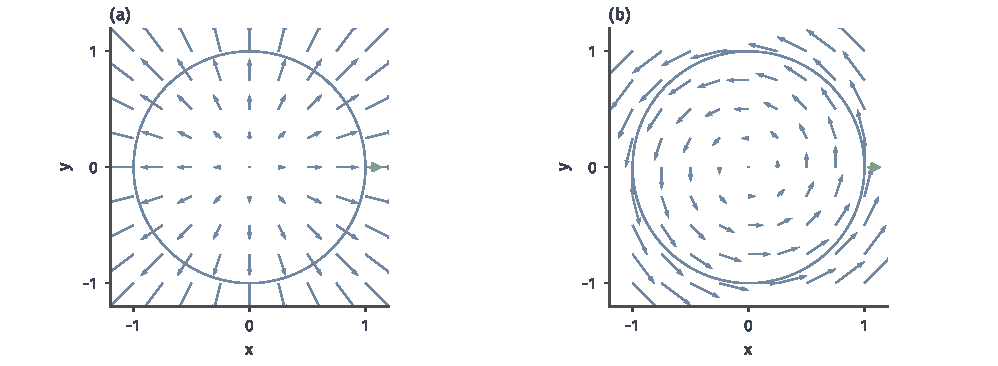
\includegraphics[width=169.0mm]{figures/01-mathematical-preliminaries-upper/01-mathematical-language-combinatorics-analysis-optimization/matplotlib/chapter3-concept-processes/divergence-circulation-fields.pdf}
 \caption{(a) 径向场$(x,y)^\top$的二维散度为$2$、旋转率$Q_x-P_y=0$，圆周外向通量为$2\pi$、环流为零。(b) 旋转场$(-y,x)^\top$的散度为零、旋转率为$2$，通量为零、环流为$2\pi$。绿箭头仅标记外法向；蓝色场箭头按相同常数缩放。零散度不等于零场，也不等于零环流。}
 \label{fig:analysis-process-divergence-circulation-fields}
\end{figure*}

\subsubsection{Laplace算子}

标量函数的梯度是向量场，因此可以对它继续取散度，把各坐标方向的二阶变化相加。
这一复合运算出现在多元分部积分中，也出现在描述热传导和扩散的方程中；它的输入与输出都是标量函数。
\begin{definition}[Laplace算子]
\label{def:multivariable-laplacian}
对开集$U\subseteq\mathbb R^d$上的二阶连续可微标量函数$v$，定义\term{Laplace算子}（Laplacian）为
\[
 \Delta v=\operatorname{div}(\nabla v)
 =\sum_{j=1}^d\partial_j^2v.
\]
\end{definition}
梯度把标量函数变为向量场，散度再把向量场变为标量函数，所以$\Delta v$仍是标量函数；它与输入、输出都是向量场的旋度属于不同类型的运算。

\paragraph{与邻域平均值的差}

一元情形中，$v''(a)>0$表示函数在$a$附近向上弯，$v(a)$低于两侧邻点的平均值。多元情形可以做同样的比较。
在$\bm a$的每个坐标方向上各取前后两个邻点$\bm a\pm h\bm e_j$，沿该坐标作二阶Taylor展开：
\[
 v(\bm a+h\bm e_j)+v(\bm a-h\bm e_j)-2v(\bm a)=h^2\partial_j^2v(\bm a)+o(h^2),
\]
一阶项$\pm h\partial_jv(\bm a)$在两点相加时抵消。对$j=1,\ldots,d$求和，再除以邻点个数$2d$，得到
\[
 \frac1{2d}\sum_{j=1}^d\bigl[v(\bm a+h\bm e_j)+v(\bm a-h\bm e_j)\bigr]-v(\bm a)
 =\frac{h^2}{2d}\Delta v(\bm a)+o(h^2).
\]
因此，$h$足够小时，$\Delta v(\bm a)>0$表示$v(\bm a)$低于周围邻点的平均值，$\Delta v(\bm a)<0$表示高于平均值；$\Delta v(\bm a)=0$表示二者之差是$o(h^2)$，在这一精度下相等。

下面用两个二次函数直接比较邻点平均值与中心值。
\begin{example}[二次函数的邻点平均]
取$v(x,y,z)=x^2+y^2+z^2$，则$\Delta v=2+2+2=6$。在原点，$v(\bm0)=0$；六个邻点$\pm h\bm e_j$上的值都是$h^2$，所以邻点平均值比中心值高$h^2$，恰等于$\frac{h^2}{2d}\Delta v=\frac{h^2}6\cdot6$。二次函数的Taylor展开没有余项，等式精确成立。

再取$v(x,y)=x^2-y^2$，则$\Delta v=2-2=0$。原点的四个邻点$(\pm h,0)$与$(0,\pm h)$上的取值为$h^2,h^2,-h^2,-h^2$，平均值恰为$0=v(\bm0)$。
\end{example}
第二个函数在$x$方向向上弯、在$y$方向向下弯，两种弯曲正好抵消。Laplace算子记录的是各坐标方向弯曲的总和，不能据此判断每个方向各自的弯曲。

\paragraph{热传导中的含义}

设$u(t,\bm x)$是时刻$t$物体内位置$\bm x$处的温度，它对$\bm x$二阶连续可微。热量从高温处流向低温处，Fourier热传导定律把单位时间穿过单位面积的热流写成$\bm q=-k\nabla u$，其中常数$k>0$为导热系数，$\nabla$只作用于空间变量$\bm x$\scite{math-openstax-calculus3}。
由散度的含义，单位体积的热量净流出率为$\operatorname{div}\bm q=-k\Delta u$。没有热源时，单位体积内热量的增加率等于净流入率$-\operatorname{div}\bm q=k\Delta u$；再除以单位体积的热容$c>0$，得到温度的变化率
\[
 \partial_tu=\frac kc\,\Delta u,
\]
这就是热传导方程。

这个方程说明温度怎样随时间变化。比周围平均更冷的点满足$\Delta u>0$，会从周围吸收热量而升温；比周围平均更热的点满足$\Delta u<0$，会降温；温度分布因而逐渐被抹平。
温度不再随时间变化时，处处有$\Delta u=0$；按邻域平均值的公式，每点的温度在上述精度下等于周围的平均。这里的Fourier定律是物理模型，本节只用它说明$\Delta$的含义。

\subsection{边界的定向}

将一个区域分成相邻小块时，公共边或公共面不属于原区域的外边界。
要使这些内部贡献相消，各小块必须采用相容的方向；同时，每个小块的方向还要与小块上局部计算所用的方向一致：环流按逆时针计算，通量按外法向计算。
下面依次规定平面区域边界的行进方向、区域边界的外法向，以及定向曲面边界的行进方向。

\subsubsection{平面区域的正向边界}

平面区域的边界是路径，所以先规定沿边界行进的方向。本节考虑的平面区域，边界由若干条简单闭曲线组成；简单闭曲线指除首尾相合外不自交的闭曲线。
对有界平面区域，取边界方向使沿曲线前进时区域总在左侧，称为正向边界。
沿单位圆逆时针行走，单位圆盘始终在左手边，所以圆盘的正向边界是逆时针方向。

有孔洞时，外边界仍是逆时针；围绕孔洞的内边界要使区域而非孔洞留在左侧，因而是顺时针。
例如圆环$1<x^2+y^2<4$的外圈$r=2$逆时针、内圈$r=1$顺时针，两圈边界方向相反。
这个约定与小块相消的要求一致：把圆环切成许多小块，每块都按逆时针走边界，内部公共边相互抵消后，剩在孔洞边上的那些边恰好被顺时针走过。

边界由多段光滑弧组成时，按这一方向逐段相接，转角处不另加积分项。
一般地，相邻平面小块各自采用正向边界时，共同边被沿相反方向走过，两个有向路径积分恰好抵消。

\subsubsection{区域边界的外法向}

通量需要的是法向，而不是边界的行进方向。空间区域的外单位法向从内部指向外部；有孔洞时，孔洞边界的外法向指向孔洞。
例如球壳$1<\lVert\bm x\rVert_2<2$在外球面上的外法向背离原点，在内球面上的外法向指向原点。
相邻子区域的公共面上，两侧子区域的外法向相反，所以内部通量相消。

平面区域边界上的外单位法向按同样方式规定，只是通量沿边界按弧长累计。
外法向与正向边界的单位切向量$\bm\tau=(\tau_1,\tau_2)^\top$有固定关系：区域在行进方向的左侧，外侧就在右侧，所以把$\bm\tau$顺时针转过直角就得到外法向$\bm n=(\tau_2,-\tau_1)^\top$。
例如在单位圆的点$(1,0)$处，逆时针的切向量是$(0,1)^\top$，按此公式得到$(1,0)^\top$，确实指向圆外。

\subsubsection{定向曲面边界的诱导方向}

曲面取定单位法向$\bm n$后，其边界路径的方向不能再任意选择。
边界的正向按右手约定确定：右手大拇指朝法向，其余手指弯曲的方向为正向，称为由法向诱导的方向，简称诱导方向。
等价地，沿边界前进并把头朝向法向时，曲面留在左侧。面朝前进方向$\bm f$、头顶朝$\bm u$站立时，左手方向是$\bm u\times\bm f$；用这个叉积可以核对具体例子。

下面用这个叉积核对两张以单位圆为边界的曲面，后面检验Stokes公式时会用到它们。
\begin{example}[向上圆盘与外向上半球面的诱导方向]
\label{ex:analysis-hemisphere-induced-orientation}
对取向上法向$\bm e_3$的单位圆盘，在边界点$(1,0,0)$处取前进方向$\bm f=\bm e_2$，左手方向为$\bm e_3\times\bm e_2=-\bm e_1$，指向圆盘内部。所以诱导方向是从上方看逆时针。

对取外法向的上半单位球面，赤道上的点$(1,0,0)$处外法向是$\bm e_1$。同样取前进方向$\bm f=\bm e_2$，左手方向为$\bm e_1\times\bm e_2=\bm e_3$，正指向半球面所在的上方。所以它的诱导方向也是从上方看逆时针，与向上圆盘的边界方向相同。
\end{example}
两张曲面在边界点处的法向不同，曲面伸出的方向也不同；但二者都满足“头朝法向时曲面在左侧”，所以诱导出同一个边界方向。

若翻转曲面法向，边界的诱导方向也随之翻转。分片曲面的定向相容，指相邻曲面片在公共边上诱导出相反的行进方向。
这时公共边上的路径积分相消，只留下整张曲面的真正边界。


图~\ref{fig:analysis-process-boundary-orientation-cancellation}把相容方向的作用画出来：只有内部公共边相消，才会只剩下整个对象的外边界。
\begin{figure}[!htbp]
 \centering
 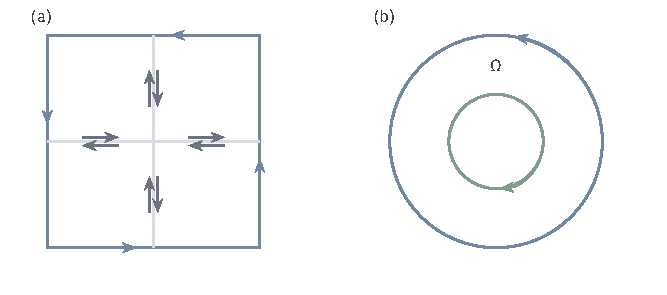
\includegraphics[width=112mm]{figures/01-mathematical-preliminaries-upper/01-mathematical-language-combinatorics-analysis-optimization/tikz/chapter3-concept-processes/boundary-orientation-cancellation.pdf}
 \caption{(a) 四个小正方形各取逆时针正向，共同边被沿相反方向走过；灰箭头略错开以便辨认，实际是同一条边。相加后只留下蓝色外边界。(b) 圆环的外边界逆时针、孔洞边界顺时针，沿任一边界前进时区域均在左侧。曲面拼片时也按公共边相反方向保证Stokes边界项相消。}
 \label{fig:analysis-process-boundary-orientation-cancellation}
\end{figure}

\subsection{平面区域积分与边界路径积分}

在平面上，区域的边界是一维路径。对同一个二维向量场，可以沿边界累计切向分量，得到环流；也可以累计外法向分量，得到通量。
两种边界积分分别对应区域内部的$Q_x-P_y$和散度$P_x+Q_y$。

\subsubsection{Green公式的环流形式}

旋度一节在小正方形上算出：逆时针环流约等于$Q_x-P_y$乘正方形面积。
把区域$\Omega$划分成许多小正方形（靠近弯曲边界处是不规则的小块），对每块写出这一近似再相加。
相邻两块的公共边在两块中方向相反，贡献抵消，剩下的只有沿$\Omega$正向边界的环流；另一侧各块“$Q_x-P_y$乘面积”之和，则是区域积分的近似和。
Green公式说明，在适当条件下这一近似在加细后成为精确等式：区域内各处微小旋转的累计，等于沿边界走一圈的总环流。
\begin{theorem}[Green公式]
\label{thm:multivariable-green}
设$\Omega\subseteq\mathbb R^2$为有界开区域，边界由有限条分段$C^1$简单闭曲线组成，
且区域在每段光滑边界附近位于边界的一侧。边界取正向，即外边界逆时针、孔洞边界顺时针。
若二维向量场$\bm F=(P,Q)^\top$在$\overline\Omega$的开邻域内连续可微，则\term{Green公式}（Green's theorem）给出
\begin{equation}
 \oint_{\partial\Omega}P\,\mathrm dx+Q\,\mathrm dy
 =\iint_\Omega\left(\frac{\partial Q}{\partial x}-\frac{\partial P}{\partial y}\right)\,\mathrm dx\,\mathrm dy.
 \label{eq:multivariable-green}
\end{equation}
\end{theorem}
左侧是向量场的切向路径积分；右侧是标量函数$Q_x-P_y$的区域积分。
在矩形上，二者的等式可以直接由一元基本定理和Fubini定理推出。
\begin{proof}[矩形情形的证明]
取$\Omega=(a,b)\times(c,d)$，先写出左侧沿四条边的贡献。下边$(t,c)$、$a\leq t\leq b$从左向右，$\mathrm dy=0$，贡献$\int_a^bP(x,c)\,\mathrm dx$；
上边从$(b,d)$走到$(a,d)$，贡献$-\int_a^bP(x,d)\,\mathrm dx$；右边从下向上，贡献$\int_c^dQ(b,y)\,\mathrm dy$；左边从上向下，贡献$-\int_c^dQ(a,y)\,\mathrm dy$。
水平边上$\mathrm dy=0$，竖直边上$\mathrm dx=0$，所以$Q$只在竖直边出现，$P$只在水平边出现。

再看右侧。场在闭矩形附近连续可微，以下被积函数均可积。固定$x$，对$y$用一元基本定理得$\int_c^d\partial_yP(x,y)\,\mathrm dy=P(x,d)-P(x,c)$；再对$x$积分，并由Fubini定理换成区域积分。对$Q$则先固定$y$、对$x$积分。于是
\[
 \begin{aligned}
 -\iint_\Omega\partial_yP\,\mathrm dx\,\mathrm dy
 &=\int_a^b[P(x,c)-P(x,d)]\,\mathrm dx,\\
 \iint_\Omega\partial_xQ\,\mathrm dx\,\mathrm dy
 &=\int_c^d[Q(b,y)-Q(a,y)]\,\mathrm dy.
 \end{aligned}
\]
第一行恰是下边与上边的两项，第二行恰是右边与左边的两项。
四项合起来，正是沿下、右、上、左四条边逆时针行进得到的路径积分。
\end{proof}
有限个矩形拼接时，公共边上的积分因方向相反而抵消。
一般规则区域的证明还需处理区域分片及边界逼近误差，不能仅凭小矩形上的等式完成；这里引用一般形式，完整论证可参考向量微积分教材\scite{math-strang1991calculus}。

先用旋转场在单位圆盘上核对公式两侧，并观察边界方向的作用。
\begin{example}[旋转场在单位圆盘上的Green公式]
\label{ex:analysis-rotation-field-green-disk}
取$\bm F=(P,Q)^\top=(-y,x)^\top$，$\Omega$为单位圆盘。$\bm F$在整个平面上连续可微，定理条件满足。
右侧被积函数为$Q_x-P_y=1-(-1)=2$，区域积分为$2\cdot\pi=2\pi$。
左侧取逆时针边界$\gamma(t)=(\cos t,\sin t)^\top$，$0\leq t\leq2\pi$，则$\bm F(\gamma(t))^\top\gamma'(t)=\sin^2t+\cos^2t=1$，积分同样为$2\pi$。
若把圆周改为顺时针，左侧变为$-2\pi$，右侧仍为$2\pi$，等式不再成立。
\end{example}
区域积分不含方向信息，边界积分却随方向反转而变号；Green公式的符号由正向边界的约定决定。

Green公式也可以反过来使用：选一个满足$Q_x-P_y\equiv1$的场，右侧就是区域的面积，于是面积可以由边界环流算出。
\begin{example}[用边界计算面积]
\label{ex:analysis-green-area-formula}
设$\Omega$满足定理~\ref{thm:multivariable-green}的条件。取$P=-y/2$、$Q=x/2$，则$Q_x-P_y=1$，Green公式给出
\[
 \operatorname{area}(\Omega)=\frac12\oint_{\partial\Omega}x\,\mathrm dy-y\,\mathrm dx.
\]
对半轴为$\alpha,\beta>0$的椭圆区域，正向边界取$\gamma(t)=(\alpha\cos t,\beta\sin t)^\top$、$0\leq t\leq2\pi$。这时$\mathrm dx=-\alpha\sin t\,\mathrm dt$、$\mathrm dy=\beta\cos t\,\mathrm dt$，
\[
 x\,\mathrm dy-y\,\mathrm dx=(\alpha\beta\cos^2t+\alpha\beta\sin^2t)\,\mathrm dt=\alpha\beta\,\mathrm dt,
\]
所以面积为$\frac12\cdot2\pi\alpha\beta=\pi\alpha\beta$。
\end{example}
这个公式只需要沿边界走一圈、记录坐标与位移，就能得到所围面积；机械求积仪正是按这一原理工作的。

定理要求场在$\overline\Omega$的开邻域内连续可微。区域包含场的奇点时，这一条件不再满足，下面的例子说明它不能省略。
\begin{example}[有孔区域上的涡旋场]
\label{ex:analysis-annulus-vortex-green}
第~\ref{sec:multivariable-potential-path-independence}节的穿孔平面反例中，$\bm F=(-y,x)^\top/(x^2+y^2)$在原点以外满足$Q_x-P_y=0$，但沿单位圆逆时针一周的环流为$2\pi$。

取圆环$\Omega=\{1<x^2+y^2<4\}$。它的闭包不含原点，$\bm F$在$\overline\Omega$的一个开邻域内连续可微，Green公式适用，右侧为$0$。
左侧由两圈组成。外圈$r=2$逆时针，参数化为$(2\cos t,2\sin t)^\top$，此时$\bm F=(-\sin t,\cos t)^\top/2$，与速度$(-2\sin t,2\cos t)^\top$的内积为$1$，环流为$2\pi$；内圈$r=1$按正向取顺时针，环流为$-2\pi$。两者相加为零，与右侧一致。
\end{example}
外圈逆时针为$2\pi$、内圈顺时针为$-2\pi$，也就是说，两条圆周按同一逆时针方向走时环流都是$2\pi$。环流来自场在原点处的奇异，而不是来自圆环内部。
单位圆盘含有原点，$\bm F$在那里无定义，不满足Green公式的条件，所以不能由$Q_x-P_y=0$推出单位圆上的环流为零。

\subsubsection{Green公式的通量形式}

现在把平面向量场想成薄层流体的速度场，问单位时间有多少流体穿过区域边界流出。
每个小正方形的净流出约等于散度乘面积；相邻两块的公共边上外法向相反，一块的流出就是另一块的流入，相加后抵消。
因此可以预期：区域内部源强度的总和，等于穿过边界的净流出。

计算通量需要把场投影到外法向上。正向边界的有向位移是$\bm\tau\,\mathrm ds=(\mathrm dx,\mathrm dy)^\top$，而外法向由$\bm\tau$顺时针转过直角得到，因此
\[
 \bm n\,\mathrm ds=(\mathrm dy,-\mathrm dx)^\top.
\]
这一关系把法向通量写成切向路径积分，从而可以使用Green公式。
\begin{theorem}[平面区域的通量公式]
\label{thm:multivariable-planar-flux}
在与Green公式相同的区域条件下，若$\bm F=(F_1,F_2)^\top$在$\overline\Omega$的开邻域内连续可微，
$\bm n$是边界的外单位法向，则
\[
 \int_{\partial\Omega}\bm F^\top\bm n\,\mathrm ds
 =\iint_\Omega\operatorname{div}\bm F\,\mathrm dx\,\mathrm dy.
\]
\end{theorem}
\begin{proof}
利用外法向与正向边界的关系，$\bm F^\top\bm n\,\mathrm ds=F_1\,\mathrm dy-F_2\,\mathrm dx$，所以左侧等于
$\oint_{\partial\Omega}(-F_2)\,\mathrm dx+F_1\,\mathrm dy$。
在Green公式中取$(P,Q)=(-F_2,F_1)$，右侧被积函数为$Q_x-P_y=\partial_xF_1+\partial_yF_2=\operatorname{div}\bm F$。
\end{proof}
这也是二维的散度公式。它与环流形式使用相同的区域条件，但累计的边界分量和内部导数不同。

下面在单位圆盘上比较两个场的通量：一个从各处均匀发散，一个只绕原点打转。
\begin{example}[单位圆盘上径向场与旋转场的通量]
取$\bm F(x,y)=(x,y)^\top$，$\Omega$为单位圆盘。散度为$1+1=2$，区域积分为$2\pi$。
边界参数化为$\gamma(t)=(\cos t,\sin t)^\top$，$0\leq t\leq2\pi$，外法向$\bm n=\gamma(t)$，$\mathrm ds=\mathrm dt$，且$\bm F^\top\bm n=\cos^2t+\sin^2t=1$，所以边界通量也为$2\pi$。若改取内法向，通量变为$-2\pi$。

再取旋转场$\bm G=(-y,x)^\top$。它的散度为$0+0=0$；在单位圆上$\bm G^\top\bm n=-y\cdot x+x\cdot y=0$，通量为零，两侧一致。它的环流却是示例~\ref{ex:analysis-rotation-field-green-disk}算出的$2\pi$。
\end{example}
径向场好比流体在圆盘内各处均匀产生，产生的总量全部从圆周流出。旋转场则像杯中被搅动的水：水在杯中打转，却没有流出杯壁。通量与环流记录的是边界上两个不同的分量。

\subsection{空间区域积分与边界曲面积分}

将平面区域换成三维空间区域后，边界从曲线变成闭曲面。
对应关系仍然是内部散度的积分等于边界净通量；由这一关系还可以推出多元函数的分部积分公式。

\subsubsection{Gauss公式}

仍把$\bm F$看作流体的速度场。区域$\Omega$内各处的散度给出单位体积的产生率，其体积积分是单位时间在$\Omega$内产生的流体总量。
流体总量守恒时，新产生的流体只能穿过边界离开，所以这个总量应等于穿过$\partial\Omega$的外向净通量。
从计算上看，把$\Omega$切成小立方体，每块的净流出约等于散度乘体积；相邻两块的公共面上外法向相反，流出与流入相消，只留下外边界上的通量。
静电学中有同样的关系：电场穿过闭曲面的通量，由闭曲面内的总电荷决定\scite{math-openstax-calculus3}。
Gauss散度定理给出这一平衡精确成立的条件。
\begin{theorem}[Gauss散度定理]
\label{thm:analysis-divergence-theorem}
设$\Omega\subseteq\mathbb R^3$为有界开区域，其边界是由有限个正则$C^1$曲面片组成的闭曲面。
各片内部互不相交，接缝为有限条分段$C^1$曲线及有限个点；在每个光滑边界点附近，区域位于边界的一侧。
若向量场$\bm F$在$\overline\Omega$的一个开邻域内连续可微，则\term{散度定理}（divergence theorem）给出
\begin{equation}
  \int_{\Omega}\nabla\mathbin{\cdot}\bm F\,\mathrm d\bm x
  =\int_{\partial\Omega}\bm F^\top\bm n\,\mathrm dS,
 \label{eq:analysis-divergence-theorem}
\end{equation}
其中$\bm n$是光滑边界片上的外单位法向，$\mathrm dS$为面积元素。
\end{theorem}
光滑有界区域和通常的多面体满足这些条件。接缝的曲面面积为零，不影响通量积分；$\bm F$及其偏导数在紧集$\overline\Omega$上连续因而有界，所以两侧积分都有限。
左侧累计向量场的局部净流出率，右侧累计穿过整个外边界的净通量。

对长方体，这一等式不需要借助一般曲面逼近，可以逐坐标证明；证明正是把散度一节中小立方体上的近似计算改写成精确等式。
\begin{proof}[长方体情形的证明]
取$\Omega=(a,b)\times(c,d)\times(e,f)$。
固定$(y,z)$，对$x$用一元基本定理，再由Fubini定理对$(y,z)$积分，得到
\[
 \int_\Omega\partial_xF_1\,\mathrm d\bm x
 =\int_c^d\int_e^f
   [F_1(b,y,z)-F_1(a,y,z)]\,\mathrm dz\,\mathrm dy.
\]
在$x=b$面上外法向为$(1,0,0)^\top$，$\bm F^\top\bm n=F_1$；在$x=a$面上外法向为$(-1,0,0)^\top$，$\bm F^\top\bm n=-F_1$。所以右侧正是这两张面的外向通量之和。
同样，$\partial_yF_2$的体积积分等于$y=d$与$y=c$两面的通量之和，
$\partial_zF_3$的体积积分等于$z=f$与$z=e$两面的通量之和。在其余各面上，相应分量与法向垂直，不贡献这一项。
三式相加，左侧为散度的体积积分，右侧为六张面的全部外向通量。
\end{proof}
拼接长方体时，公共面上的外法向相反，内部通量恰好抵消。
从长方体推广到定理中的一般规则区域，还需对边界分片和逼近作严格处理；一般形式在这里引用，证明可参考向量微积分教材\scite{math-strang1991calculus}。
无界区域、弱导数或更不规则的边界，需要另用相应版本，不能由长方体情形直接推出。


图~\ref{fig:analysis-process-gauss-shared-face}显示体积小块相加时，共同面上的两份通量为什么消失。
\begin{figure}[!htbp]
 \centering
 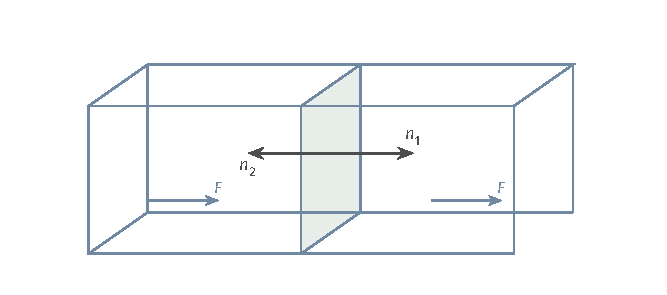
\includegraphics[width=112mm]{figures/01-mathematical-preliminaries-upper/01-mathematical-language-combinatorics-analysis-optimization/tikz/chapter3-concept-processes/gauss-shared-face.pdf}
 \caption{两个相邻单位立方体共用绿色面，图用斜投影表示三维几何。取常场$F=(1,0,0)^\top$，共同面上两侧外法向为$n_1=(1,0,0)^\top$与$n_2=-n_1$，对应通量为$1,-1$，相加抵消。整体外向净通量也为零，与散度为零一致；一般区域的散度定理仍需要前述条件与证明。}
 \label{fig:analysis-process-gauss-shared-face}
\end{figure}

先用一个答案已知的计算核对散度定理。
\begin{example}[用散度定理核对球面面积]
设$B_R$是以原点为中心、半径$R>0$的球，边界球面取外法向。令$\bm F(\bm x)=\bm x/R$，它在整个$\mathbb R^3$上连续可微。
球面上$\bm n=\bm x/R=\bm F$，所以$\bm F^\top\bm n=1$，外向通量等于球面面积。
另一方面，$\operatorname{div}\bm F=3/R$，散度定理给出
\[
 \int_{\partial B_R}\bm F^\top\bm n\,\mathrm dS
 =\frac3R\operatorname{vol}(B_R)
 =\frac3R\cdot\frac{4\pi R^3}3=4\pi R^2.
\]
\end{example}
这里的球体积已在第~\ref{sec:multivariable-change-variables}节用球坐标算出；所得结果与第~\ref{sec:analysis-surface-integration}节直接参数化球面求得的面积一致。

定理要求$\bm F$在$\overline\Omega$的一个开邻域内连续可微。点源场在原点无定义，下面用它检查这一条件的作用。
\begin{example}[点源的通量]
\label{ex:analysis-point-source-flux}
在$\mathbb R^3\setminus\{\bm0\}$上取$\bm F(\bm x)=\bm x/\lVert\bm x\rVert_2^3$，记$r=\lVert\bm x\rVert_2$。由$\partial_jr=x_j/r$，
\[
 \partial_j\Bigl(\frac{x_j}{r^3}\Bigr)=\frac1{r^3}-\frac{3x_j^2}{r^5},
 \qquad
 \operatorname{div}\bm F=\frac3{r^3}-\frac{3r^2}{r^5}=0.
\]
但在半径为$R$的球面上，外法向为$\bm x/R$，$\bm F^\top\bm n=1/R^2$，外向通量为$4\pi R^2/R^2=4\pi$。
这并不与散度定理矛盾：球体含有原点，而$\bm F$在原点无定义，定理的条件不满足。

对不含原点的球壳$R_1<r<R_2$，定理适用，左侧为零。外球面的外向通量为$4\pi$；内球面的外法向指向原点，通量为$-4\pi$；两者相加确为零。
\end{example}
所以以原点为中心的球面上的通量都是$4\pi$，与半径无关：场在原点以外处处无源，全部通量都来自原点处的点源。
静电学中，位于原点的点电荷$q$产生的电场是$\frac{q}{4\pi\varepsilon_0}\bm F$，其中$\varepsilon_0$为真空介电常数；它穿过以原点为中心的球面的通量为$q/\varepsilon_0$，这就是Gauss定律在点电荷上的形式。

\paragraph{散度是通量密度}

已证明的长方体情形，足以把散度一节的近似推导变成精确结论。
设$\bm F$在开集$U$上连续可微，$\bm a\in U$，$Q_h$是以$\bm a$为中心、边长为$h$的立方体；$h$足够小时$\overline{Q_h}\subseteq U$。由长方体上的Gauss公式，
\[
 \frac1{h^3}\int_{\partial Q_h}\bm F^\top\bm n\,\mathrm dS
 =\frac1{h^3}\int_{Q_h}\operatorname{div}\bm F\,\mathrm d\bm x.
\]
右侧是散度在$Q_h$上的平均值，它与$\operatorname{div}\bm F(\bm a)$的差不超过$\sup_{Q_h}|\operatorname{div}\bm F-\operatorname{div}\bm F(\bm a)|$。散度连续，所以$h\to0$时这个上界趋于零，平均值趋于$\operatorname{div}\bm F(\bm a)$。

这说明散度确实是“单位体积的净流出”的极限。把立方体换成以$\bm a$为中心的小球，用一般的Gauss公式可以得到同样的极限。小球的取法不依赖坐标轴，所以散度描述的是场本身的性质，不依赖坐标系的方向。

\subsubsection{多元分部积分}

一元分部积分（式~\eqref{eq:analysis-integration-by-parts}）把一个因子的导数转给另一个因子，并留下端点项。设$u$在$[a,b]$上连续可微、$v$二阶连续可微，把式中的$v$换成$v'$，得到
\[
 \int_a^bu\,v''\,\mathrm dx
 =u(b)v'(b)\cdot(+1)+u(a)v'(a)\cdot(-1)-\int_a^bu'v'\,\mathrm dx.
\]
这里把端点项$[uv']_a^b$拆开写：区间在右端点的外法向是$+1$，在左端点是$-1$。

推广到多元情形时，各项依次对应：二阶导数$v''$换成$\Delta v$，一阶导数的乘积$u'v'$换成梯度的内积$\nabla u^\top\nabla v$，两个端点换成边界曲面，“$v'$乘外法向$\pm1$”换成$\nabla v^\top\bm n$，即$v$沿外法向的方向导数。
对乘积向量场$u\nabla v$使用散度定理，就得到这一推广。
\begin{theorem}[多元分部积分]
\label{thm:multivariable-integration-by-parts}
设$\Omega\subseteq\mathbb R^3$满足上述Gauss公式的区域条件。
若标量函数$u$在$\overline\Omega$的开邻域内连续可微，$v$在同一邻域内二阶连续可微，则
\[
 \int_\Omega u\Delta v\,\mathrm d\bm x
 =\int_{\partial\Omega}u\nabla v^\top\bm n\,\mathrm dS
  -\int_\Omega\nabla u^\top\nabla v\,\mathrm d\bm x.
\]
\end{theorem}
\begin{proof}
向量场$\bm F=u\nabla v$的第$j$个分量是$u\,\partial_jv$，它连续可微。由一元乘积法则，
$\partial_j(u\,\partial_jv)=\partial_ju\,\partial_jv+u\,\partial_j^2v$，对$j$求和得到
\[
 \operatorname{div}(u\nabla v)
 =\nabla u^\top\nabla v+u\Delta v.
\]
将它代入Gauss公式，再把$\nabla u^\top\nabla v$的区域积分移到等式另一侧，即得结论。
\end{proof}
对满足Green公式条件的平面区域，同样的证明改用平面通量公式（定理~\ref{thm:multivariable-planar-flux}）即可，边界面积元素相应换成弧长元素。
这一公式把$v$的二阶导数转移为$u$与$v$的一阶导数，同时保留法向边界项；该项是否为零，必须由具体边界条件决定。

取$u=1$，公式化为$\int_\Omega\Delta v\,\mathrm d\bm x=\int_{\partial\Omega}\nabla v^\top\bm n\,\mathrm dS$，也就是对梯度场$\nabla v$使用散度定理。下面在球上核对这一特例。
\begin{example}[球上平方范数的Laplace积分]
取以原点为中心、半径为$R$的球$B_R$和$v(\bm x)=\lVert\bm x\rVert_2^2$。
左侧：$\Delta v=6$，所以$\int_{B_R}\Delta v\,\mathrm d\bm x=6\operatorname{vol}(B_R)=6\cdot\frac{4\pi R^3}3=8\pi R^3$。
右侧：球面上$\nabla v=2\bm x$，外法向$\bm n=\bm x/R$，故$\nabla v^\top\bm n=2\lVert\bm x\rVert_2^2/R=2R$，积分为$2R\cdot4\pi R^2=8\pi R^3$。两侧相等。
\end{example}

边界项为零时，公式可以给出结构性的结论。下面用它说明Laplace方程的解由边界值唯一确定。
\begin{example}[Laplace方程的解由边界值决定]
设$\Omega$满足Gauss公式的区域条件，$w$在$\overline\Omega$的开邻域内二阶连续可微，在$\Omega$内$\Delta w=0$，在$\partial\Omega$上$w=0$。
在定理~\ref{thm:multivariable-integration-by-parts}中取$u=v=w$。左侧被积函数$w\Delta w$为零；边界项的被积函数含因子$w$，也为零。于是
\[
 \int_\Omega\lVert\nabla w\rVert_2^2\,\mathrm d\bm x=0.
\]
被积函数连续且非负；若它在某点为正，则在该点的一个邻域内为正，积分也为正。所以在开集$\Omega$上$\nabla w$恒为零。
$\Omega$是连通的开区域，所以$w$在$\Omega$上为常数；再由$w$在$\overline\Omega$上连续且在边界上为零，得$w\equiv0$。

现在设$v_1,v_2$都在$\overline\Omega$的开邻域内二阶连续可微，在$\Omega$内满足$\Delta v_1=\Delta v_2=0$，在$\partial\Omega$上取值相同。差$w=v_1-v_2$满足上面的全部条件，所以$v_1=v_2$。
\end{example}
按热传导的解释，稳定的温度分布由边界温度唯一决定。

\subsection{曲面积分与边界路径积分}

Gauss公式要求闭曲面围成空间区域。另一类问题只给一张有边界的定向曲面，要求比较曲面上的旋转累计与边界环流。
这时使用旋度在曲面法向上的分量，不需要先把曲面补成闭曲面。

\subsubsection{Stokes公式}

在$z=0$平面上取向上法向时，旋度的法向分量$(\nabla\times\bm F)^\top\bm e_3$就是Green公式中的$Q_x-P_y$。
对空间中的弯曲曲面，可以把它切成许多很小的曲面片，每片近似是一小块平面。在法向为$\bm n$的小平面片上，边界环流约等于$(\nabla\times\bm F)^\top\bm n$乘面积。
各片采用相容定向时，相邻两片的公共边被沿相反方向走过，环流相消，只剩整张曲面的边界。
用桨轮的图像说：在曲面上各处放置转轴沿法向的小桨轮，它们感受到的旋转强度按面积累加，总和等于沿曲面边缘走一圈的环流。
Stokes公式把这一关系写成精确等式，同时要求法向与边界方向相容。
\begin{theorem}[Stokes定理]
\label{thm:multivariable-stokes}
设$S\subseteq\mathbb R^3$为紧致、可定向的分片$C^2$曲面，边界由有限条分段$C^1$简单闭曲线组成。
各光滑曲面片选取连续且片间定向相容的单位法向$\bm n$，边界采用其诱导方向。
若向量场$\bm F$在$S$的开邻域内连续可微，则\term{Stokes公式}（Stokes' theorem）给出
\begin{equation}
 \oint_{\partial S}\bm F^\top\,\mathrm d\bm r
 =\int_S(\nabla\times\bm F)^\top\bm n\,\mathrm dS.
 \label{eq:multivariable-stokes}
\end{equation}
\end{theorem}
这里的“可定向”要求各曲面片能相容地选择法向，使公共边上的诱导方向相反；有折角的接缝处不要求存在唯一法向。
两侧都为标量：左侧是原向量场的边界环流，右侧是其旋度穿过曲面的通量。

在一张参数曲面片上，可以把公式归结为参数平面上的Green公式。
设参数域$D$满足Green公式的区域条件，$\bm r(u,v)$在$D$的邻域内二阶连续可微、在内部正则且一一对应，并采用$\bm r_u\times\bm r_v$确定的定向。
还要求$\partial D$的正向经$\bm r$对应曲面片边界的诱导方向，从而可以把边界路径积分放到$\partial D$上计算。
这里的$u,v$是参数，与多元分部积分中的函数$u,v$无关。记
\[
 \begin{aligned}
 A(u,v)&=\bm F(\bm r(u,v))^\top\bm r_u(u,v),\\
 B(u,v)&=\bm F(\bm r(u,v))^\top\bm r_v(u,v).
 \end{aligned}
\]

先处理左侧。若$(u(t),v(t))$沿$\partial D$行进，曲面边界上对应的点是$\bm r(u(t),v(t))$，由链式法则，其速度为$\bm r_uu'(t)+\bm r_vv'(t)$。
与$\bm F$取内积，得$\bm F^\top\mathrm d\bm r=A\,\mathrm du+B\,\mathrm dv$，所以左侧等于参数平面上的路径积分$\oint_{\partial D}A\,\mathrm du+B\,\mathrm dv$。

再计算参数平面上Green公式右侧的被积函数$\partial_uB-\partial_vA$。记$\bm J_{\bm F}$为$\bm F$的Jacobian矩阵，其元素为$(\bm J_{\bm F})_{i,j}=\partial_jF_i$。由链式法则和乘积法则，
\[
 \begin{aligned}
 \partial_uB&=(\bm J_{\bm F}\bm r_u)^\top\bm r_v+\bm F^\top\bm r_{vu},\\
 \partial_vA&=(\bm J_{\bm F}\bm r_v)^\top\bm r_u+\bm F^\top\bm r_{uv},
 \end{aligned}
\]
其中$\bm J_{\bm F}$与$\bm F$在$\bm r(u,v)$处取值。$\bm r$二阶连续可微，混合偏导相等，$\bm r_{uv}=\bm r_{vu}$，所以两式相减时含二阶导数的项抵消。
又$(\bm J_{\bm F}\bm r_u)^\top\bm r_v=\bm r_v^\top\bm J_{\bm F}\bm r_u$、$(\bm J_{\bm F}\bm r_v)^\top\bm r_u=\bm r_v^\top\bm J_{\bm F}^\top\bm r_u$，于是
\[
 \partial_uB-\partial_vA=\bm r_v^\top(\bm J_{\bm F}-\bm J_{\bm F}^\top)\bm r_u.
\]

接下来把右端写成旋度。反对称矩阵$\bm W=\bm J_{\bm F}-\bm J_{\bm F}^\top$的元素为$\bm W_{i,j}=\partial_jF_i-\partial_iF_j$；逐个分量对照旋度的定义可以验证，对任意$\bm a\in\mathbb R^3$都有$\bm W\bm a=(\nabla\times\bm F)\times\bm a$。
再用混合积的轮换关系$\bm b^\top(\bm c\times\bm a)=\bm c^\top(\bm a\times\bm b)$（两边都等于以$\bm a,\bm b,\bm c$为列的行列式），取$\bm a=\bm r_u$、$\bm b=\bm r_v$、$\bm c=\nabla\times\bm F$，得到
\[
 \partial_uB-\partial_vA
 =\bigl(\operatorname{curl}\bm F\bigr)(\bm r(u,v))^\top
   (\bm r_u\times\bm r_v).
\]
右端乘$\mathrm du\,\mathrm dv$，正是曲面通量积分（式~\eqref{eq:analysis-surface-flux}）中的被积项。

$A,B$由连续可微的$\bm F$与二阶连续可微的$\bm r$及其一阶导数复合、相乘而成，在$D$的邻域内连续可微，所以参数平面上的Green公式适用；它给出该曲面片上的Stokes公式。
对有限张相容定向的曲面片，公共边的路径积分相消，只剩整张曲面的边界。
一般分片曲面的完整论证还需核对曲面覆盖及接缝条件；以上推导只说明参数片上的机制，一般定理可参考向量微积分教材\scite{math-strang1991calculus}。

\paragraph{旋度分量是环流密度}

Stokes公式也给出旋度含义的精确形式。设$\bm F$在$\bm a$附近连续可微，$\bm n$是单位向量，$D_\rho$是以$\bm a$为圆心、半径为$\rho$、垂直于$\bm n$并取法向$\bm n$的平面圆盘。由Stokes公式，
\[
 \frac1{\pi\rho^2}\oint_{\partial D_\rho}\bm F^\top\,\mathrm d\bm r
 =\frac1{\pi\rho^2}\int_{D_\rho}(\nabla\times\bm F)^\top\bm n\,\mathrm dS,
\]
右侧是$(\nabla\times\bm F)^\top\bm n$在圆盘上的平均值。旋度连续，所以$\rho\to0$时它趋于$(\nabla\times\bm F)(\bm a)^\top\bm n$。
因此，旋度沿$\bm n$的分量就是垂直于$\bm n$的微小圆周上的环流除以所围面积的极限。这正是桨轮图像所描述的量；圆盘的取法不依赖坐标轴，所以这一含义也不依赖坐标轴的选取。

\subsubsection{跨接曲面的选择}

Stokes公式的左侧只由有向边界和边界上的向量场决定。因此，若两张满足定理条件的定向曲面具有同一有向边界，
且$\bm F$在两张曲面附近都连续可微，则两张曲面上的旋度通量相等。
计算时可以选较简单的跨接曲面，但必须核对向量场定义域，不能让替换曲面穿过场的奇点。

这一结论也可以从Gauss公式得到印证。若$\bm F$二阶连续可微，则
\[
 \operatorname{div}(\nabla\times\bm F)
 =\partial_x(\partial_yF_3-\partial_zF_2)
 +\partial_y(\partial_zF_1-\partial_xF_3)
 +\partial_z(\partial_xF_2-\partial_yF_1)=0,
\]
最后的等号成立，是因为混合偏导相等，六项两两抵消。设两张跨接曲面恰好围成一个满足Gauss公式条件的区域，且$\bm F$在该区域闭包的开邻域内二阶连续可微。
区域的外法向在一张曲面上与所选法向相同，在另一张上相反；旋度场的散度为零，所以散度定理说明两张曲面上的旋度通量之差为零。

下面用同一个场在单位圆上比较两张跨接曲面。
\begin{example}[单位圆上的圆盘与半球面]
取$\bm F=(-y/2,x/2,0)^\top$，它在整个$\mathbb R^3$上连续可微，示例~\ref{ex:analysis-rigid-rotation-curl}已算出$\nabla\times\bm F=(0,0,1)^\top$。单位圆$\{x^2+y^2=1,\ z=0\}$采用从上方看逆时针的方向。

先取向上单位圆盘$S_1$。由示例~\ref{ex:analysis-hemisphere-induced-orientation}，它的诱导方向正是这一方向；旋度的法向分量为$1$，所以
\[
 \oint_{\partial S_1}\bm F^\top\,\mathrm d\bm r
 =\iint_{S_1}1\,\mathrm dS=\pi.
\]
直接计算左侧也得到同一结果：取$\gamma(t)=(\cos t,\sin t,0)^\top$，$0\leq t\leq2\pi$，则$\bm F(\gamma(t))^\top\gamma'(t)=\tfrac12(\sin^2t+\cos^2t)=\tfrac12$，积分为$\pi$。

再取外向上半单位球面$S_2$，同一例子说明它的诱导方向与$S_1$相同。用第~\ref{sec:analysis-surface-integration}节的球面参数$(\varphi,\theta)$，$0\leq\varphi\leq\pi/2$，外法向为$\bm n=\bm x$，旋度的法向分量为$z=\cos\varphi$，面积元为$\sin\varphi\,\mathrm d\varphi\,\mathrm d\theta$，所以
\[
 \int_{S_2}(\nabla\times\bm F)^\top\bm n\,\mathrm dS
 =\int_0^{2\pi}\int_0^{\pi/2}\cos\varphi\sin\varphi\,\mathrm d\varphi\,\mathrm d\theta
 =2\pi\cdot\frac12=\pi,
\]
与圆盘上的结果相同。
\end{example}
若改用向下定向的圆盘，边界方向也必须反转，两个积分同时变号。


图~\ref{fig:analysis-process-stokes-spanning-surfaces}比较同一有向圆周的两张跨接曲面。替换曲面时，边界方向与场的定义域都要同时保留。
\begin{figure*}[!htbp]
 \centering
 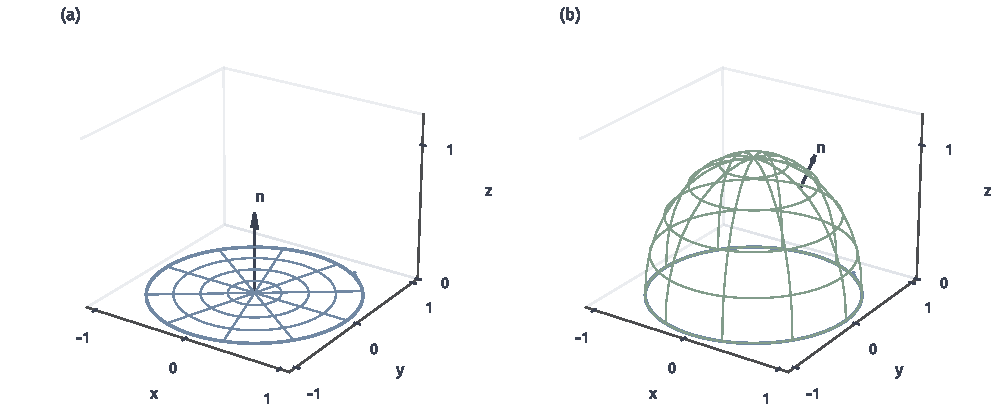
\includegraphics[width=169.0mm]{figures/01-mathematical-preliminaries-upper/01-mathematical-language-combinatorics-analysis-optimization/matplotlib/chapter3-concept-processes/stokes-spanning-surfaces.pdf}
 \caption{(a) 向上单位圆盘；(b) 外向上半单位球面。蓝色边界均从上方看逆时针，黑箭头标记各自法向。对$F=(-y/2,x/2,0)^\top$，旋度恒为$(0,0,1)^\top$，两面上的旋度通量都为$\pi$。右面面积为$2\pi$而非$\pi$；相等的是法向分量的累计，不能把通量当成面积。}
 \label{fig:analysis-process-stokes-spanning-surfaces}
\end{figure*}

\subsection{积分公式的比较}

本节各公式回答的都是同一类问题：导数在内部的积分与边界积分之间的关系。推导方式也相同：在小块上建立局部关系，再利用相容方向让内部边界相消。
它们的内部对象、边界对象和方向条件则各不相同。下表把一元基本定理与路径积分基本定理也列在一起，二者以区间或路径的两个端点为边界。
\begin{center}
\begin{tabular}{lll}
\toprule
公式 & 内部积分 & 边界积分\\
\midrule
一元基本定理 & 区间上的$f'$ & 端点值之差$f(b)-f(a)$\\
路径积分基本定理 & 路径上$\nabla\phi$的切向积分 & 端点值之差\\
Green环流形式 & 平面区域的$Q_x-P_y$ & 正向路径的切向积分\\
Gauss & 空间区域的散度 & 闭曲面的外向通量\\
Stokes & 定向曲面的旋度通量 & 诱导方向的路径环流\\
\bottomrule
\end{tabular}
\end{center}
对向上定向的平面曲面，Stokes公式还原为Green公式的环流形式；Green公式的通量形式则是二维的散度公式。
普通标量函数的区域积分不自动具有边界表达：要使用这些公式，须先找到满足条件的向量场，使其散度或旋度的相应分量等于被积函数。示例~\ref{ex:analysis-green-area-formula}的面积公式就是先选出满足$Q_x-P_y\equiv1$的场。

Stokes公式还解释了第~\ref{sec:multivariable-potential-path-independence}节中势函数的存在为何与定义域有关。设$\bm F$在开集$U\subseteq\mathbb R^3$上连续可微且$\nabla\times\bm F=\bm0$。若一条闭路径是$U$内某张满足定理条件的定向曲面的有向边界，则该闭路径上的环流等于旋度的通量，也就是零。
在星形域中，闭路径上各点与中心点之间的线段扫出一张锥面，它整个落在定义域内，不会碰到场的奇点；这与那里在星形域上构造势函数的结论一致。
穿孔平面上绕原点的单位圆则不同：在平面内，以它为边界的区域只能是单位圆盘，必然包含原点，而场在原点无定义；所以局部条件$Q_x-P_y=0$并不排除$2\pi$的环流（示例~\ref{ex:analysis-annulus-vortex-green}）。

各公式均使用勒贝格积分。连续可微性、分片规则边界与定向是这里的经典公式所需的条件，并不是另换一种积分定义。
尤其要核对向量场是否在整个积分对象附近都有定义：穿孔平面上的涡旋场在原点无定义，不能把包含原点的圆盘直接代入Green公式；点源场也不能直接用于包含原点的球体（示例~\ref{ex:analysis-point-source-flux}）。
区域积分不能区分只在零测集上不同的函数，而本节区域的边界由有限条曲线或有限个曲面片组成，在相应的面积或体积测度下正是零测集；所以仅知道两个函数在区域上几乎处处相等，不足以确定它们的边界积分。
如果要降低导数或边界的规则性，还须另外建立弱导数、边界迹及相应的积分公式；不能沿用当前公式而省去这些条件。

\FloatBarrier


\FloatBarrier
\section{本章小结}
\label{sec:multivariable-summary}

多元可微性要求所有小扰动共享同一个线性映射，仅有坐标切片或各个固定方向的信息还不够。
区域、路径与曲面累计分别使用体积、弧长和曲面面积，有向路径与通量还保留方向。
Tonelli与Fubini定理控制逐坐标累计，Jacobian校正坐标变换的体积。
Green、Gauss和Stokes公式把特定导数的内部累计联系到边界，扩展一元微积分基本定理，
也各自要求明确的正则性、可积性和定向条件。

